\documentclass[11pt, a4paper,oneside,openright]{book}

\usepackage{amssymb}
\usepackage{amsmath}
\usepackage{graphicx}
\usepackage{multirow}
\usepackage{hyperref}
\hypersetup{
  colorlinks=false,
  citecolor=green,
  filecolor=black,
  linkcolor=red,
  urlcolor=cyan
  }

\addtolength{\hoffset}{-2.5cm}
\addtolength{\textwidth}{4.5cm}
\addtolength{\voffset}{-2cm}
\addtolength{\textheight}{4.5cm}

\numberwithin{equation}{section}

\begin{document}

\title{An introductory class to Physical Cosmology for the Science Honors Program}
\author{Sebastian Garcia-Saenz and Andrea Petri}
\date{Columbia University in the City of New York}
\maketitle

\chapter*{Introduction}
Physical Cosmology is the science that studies the universe on its largest scales, much bigger that planets, planetary systems and even galaxies; on these big scales the universe is well approximated by a nearly homogeneous fluid with very small inhomogeneities. This picture is strongly supported by the last two decades of observations of the Cosmic Microwave Background (CMB), a radiation leftover from the Big Bang whose established presence is the main invitation for the developement and study of Cosmology itself. These notes are meant to be a quick overview of this subject, rolling over its most important and interesting aspects. It will be clear from the beginning that classical physics  is not fit for describing the universe at these large scales, so first we need to introduce the necessary tools for an appropriate description of Cosmology, namely Einstein's theory of Relativity (both special and general). Even if this class is not meant to be technical but qualitative, focusing on the physical ideas, we 
first need to introduce some basic mathematical tools needed for a first understanding. Next we will talk about Relativity, again not technically, but focusing on the physical ideas, at the simplest mathematical level allowed; we then start talking about Cosmology, introducing the Friedmann model that describes the homogeneous universe. To fully understand the physics at this level, we will need to know what this universe, in which we live, is made of, and this will lead us in talking about elementary particles and the thermal history of the cosmos from the Big Bang to the present time; we will try to understand the concepts of dark matter, dark energy, and the importance of the CMB in this big picture. By then we will be able to talk about inhomogeneities, the appearence of large scale structure, dark matter filaments, cluster of galaxies, galaxies and stars. The class will end with an overview of some special topics which are deeply connected with Cosmology, such as black holes, active galactic nuclei and 
the concept of inflation. 

\tableofcontents

\chapter{Preliminary tools: units, vectors, calculus, Newton's laws}

\section{Measurements and measure units}
In physics (as in any science), each time we want to express the result of a measurement we must always specify its \textit{measure unit}, i.e. a standard quantity to refer to when quoting a result; in setting the standard of measure units, the \textit{International System of Units} (or SI) helps us, defining seven fundamental units for the corresponding physical quantities

\begin{table}[htdp]
\begin{center}
\begin{tabular}{|c|c|c|} \hline
\textbf{Quantity} & \textbf{Unit(name)} & \textbf{Unit(symbol)} \\ \hline
Length & meter & m \\ \hline
Time & second & s \\ \hline
Mass & kilogram & kg \\ \hline
Temperature & kelvin & K \\ \hline
Electric current & ampere & A \\ \hline
Amount of substance & mole & mol \\ \hline
Luminous intensity & candle & cd \\ \hline
\end{tabular}
\end{center}
\caption{A list of the SI measure units}
\end{table}

\noindent From these, we can build countless derived measure units, and what follows are just some examples; for the purpose of this class, we want to quote for convenience some other standard units derived from these, that we will make use of frequently
\begin{table}[htdp]
\begin{center}
\begin{tabular}{|c|c|c|c|} \hline
\textbf{Name} & \textbf{Comments} & \textbf{Symbol} & \textbf{Approximate value} \\ \hline
Speed of light &Einstein's pride & $c$ & $3\cdot 10^8$m/s \\ \hline
Light year &$c\,\,\times$ 1\,year& ly & 9.5$\cdot10^{15}$m\\ \hline
Hubble constant &Fundamental quantity in cosmology&$H_0$&$10^{-10}$yr$^{-1}$\\ \hline
Parsec &Cosmological length scale& pc & 3ly \\ \hline
Hubble horizon &Size of the observable universe today& $d_H$&3Gpc\\ \hline 
Solar mass & Mass of the sun & $M_\odot$ & 2$\cdot10^{30}$ kg\\ \hline
CMB temperature &Observed temperature of the background radiation&$T_{CMB}$&2.78 K \\ \hline 

\end{tabular}
\end{center}
\caption{Some useful quantities that occur frequently in Cosmology}
\end{table}

\section{Organizing physical quantities: scalars, vectors and tensors}
Cosmology, as a part of physics, is a scientific theory that is formulated in terms of precise mathematical terms; these concepts help exemplify the reasonments, which would be much complicated if tried to be explained in terms of pure words, and help develop the same reasonments more naturally. In this section, we want to introduce the basic mathematical framework with which physical quantities are usually described. We saw before that any physical quantity is associated with its proper measure unit; there is more: we distinguish physical quantities in three main categories, namely \textit{scalars}, \textit{vectors} and \textit{tensors}. 
\subsection{Scalars}
We give the name \textit{scalar} to all physical quantities that can be completely characterized by only one number; for example, when we talk about the mass of a body, or a planet, or a star, we know that this mass can be completely described by only one number, with its measure unit. For example, the mass of the sun is given by $M_\odot\approx 2\cdot 10^{30}$\,kg. We can try to push this definition a little bit further, saying that a \textit{scalar} is a quantity that is \textit{invariant} (i.e. does not change) under rotations. Thinking about the sun, we can safely say in fact that its mass certainly does not depend on the direction we look at it (invariance under rotations). 
\subsection{Vectors}
Not all the quantities in physics are scalars: for example, when we need to describe a body that moves (it can be the earth orbiting the sun), we need to specify a number that describes the magnitude of its velocity $v$, but that's not all, cause to completely characterize its velocity we also need to specify its \textit{direction}. This can be done specifying the three numbers $\mathbf{v}=(v_x,v_y,v_z)$, which are the components of the velocity $\mathbf{v}$ along the three axes $x,y,z$. This quantity $\mathbf{v}$, that carries information on the direction of the motion is called a \textit{vector}, and can be indicated in bold, $\mathbf{v}$, or with the notation $v_i$, with the index $i$ being one between $x,y,z$ or $1,2,3$. Let's examine what happens under rotations: we cannot say anymore that the components $v_i$ are invariant under rotations, because if we rotate our $(x,y,z)$ axes, the components will change as well. When we perform an axes' rotation the velocity components (and in general any vector 
components) will change from $v_i$ to $v'_i$ with
\begin{equation}
v'_i=\sum_{j=1}^3R_{ij}v_j
\end{equation}
Being $R_{ij}$ an appropriate matrix of real numbers; each quantity that transforms in such a way (only involving linear terms, not $v^2,v^3,...$) is called a \textit{vector}. If we are provided two vectors $\mathbf{a},\mathbf{b}$, we can easily build a scalar $s$ out of them with the following operation called \textit{scalar product}
\begin{equation}
\label{scalarprod}
s=\mathbf{a}\cdot\mathbf{b}\equiv \sum_{i=1}^3a_ib_i
\end{equation}
This quantity $s$ so defined is a true scalar, in the sense that it's invariant under rotations; think about the following examples
\begin{itemize}
\item Let a body move with velocity $\mathbf{v}$; the magnitude of its velocity $v=\sqrt{\mathbf{v}\cdot{\mathbf{v}}}$ is obviously rotation invariant
\item Let a body move with velocity $\mathbf{v}$ and another body move with velocity $\mathbf{u}$; their directions of motion form an angle $\theta$ given by
\begin{equation}
\cos{\theta}=\frac{\mathbf{v}\cdot\mathbf{u}}{vu}
\end{equation}
which is clearly rotation invariant
\end{itemize}
\subsection{Tensors}
The natural extension of the concept of vector, considering rotation properties, is that of \textit{tensor}: if a vector is a triplet of numbers $v_i$ that transforms under a rotation $\mathbf{R}$ in the way
\begin{equation}
v'_i=\sum_{j=1}^3R_{ij}v_j
\end{equation} 
we can define a \textit{tensor} (with two indices) $T_{ij}$ ($i,j=1,2,3$) as an object that transforms not with one but two $\mathbf{R}$ matrices
\begin{equation}
T'_{ij}=\sum_{l,m=1}^3R_{il}R_{jm}T_{lm}\equiv R_{il}R_{jm}T_{lm}
\end{equation}
Where the last $\equiv$ means that we adopted a particular convention where if an index appears twice, we must sum over all possible values of that index (example sum over $m=1,2,3$ and $l=1,2,3$). We can easily generalize this definition to tensors with more than two indices; as an invitation, keep in mind that these concepts are really useful to describe spacetime and gravity in the Einstein's way. For example the metric of the spacetime, that describes its geometry, is a tensor with two indices (usually denoted with $g_{\mu\nu}$) while the Riemann tensor, which describes the curvature of spacetime, is a tensor with four indices (usually denoted with $R_{\mu\nu\rho\sigma}$) with $\mu,\nu,\rho,\sigma=0,1,2,3$ with the added 0-th component as time. 

\section{A little bit of calculus}
The reason for introducing calculus tools and techniques in physics and cosmology, is that usually physical quantities, let them be scalars (temperature, density,...), vectors (velocity, gravitational field, ...) or tensors (metric, curvature,...), are usually space and time dependent. We then need an efficient mathematical tool to understand how these quantities \textit{change} in space and time; we introduce then the concepts of \textit{derivative} and \textit{integral}. 
\subsection{Derivatives}
Let be $\mathbf{x}=(x,y,z)$ be a generic point in space and $f(\mathbf{x})$ \textit{any} physical quantity (can be scalar, vector or tensor) that depends on the position where we are in space (it can be the temperature of the air in a room, the velocity of the water on the sea, the curvature of space due to a planet, etc). Since in general $f(\mathbf{x}_1)\neq f(\mathbf{x}_2)$, we want to quantify how different are these two quantities. We usually do that computing the difference $f(\mathbf{x}_1)-f(\mathbf{x}_2)$, and this gives us an idea on how big is the difference between $f$ in two different positions; the concept of \textit{derivative} is simply the expression of this concept but when the two points $\mathbf{x}_1,\mathbf{x}_2$ are really close to each other $\mathbf{x}_1\approx\mathbf{x}_2$. In this case we can approximate 
\begin{equation}
f(\mathbf{x}_1)-f(\mathbf{x}_2)\approx \nabla f(\mathbf{x}_1)\cdot(\mathbf{x}_1-\mathbf{x}_2)
\end{equation}
Where $\nabla f(\mathbf{x})$ is called \textit{derivative} or \textit{gradient} of the quantity $f$ at the point $\mathbf{x}$ and expresses the \textit{rate of change} of $f$ at $\mathbf{x}$
\subsubsection{Note 1}
If instead of space, our quantity $f$ depends on time $t$, the definition is even simpler, but in this case we use the notation
\begin{equation}
f(t_1)-f(t_2)\approx f'(t_1)(t_1-t_2)
\end{equation}
Where we indicated the derivative at $t_1$ as $f'(t_1)$; to make the previous approximate relation more exact, we can take into account that also the derivative $f'$ varies on time, and construct a \textit{second derivative} $(f')'\equiv f''$. It is claimed that any (well behaved) quantity can be approximated as 
\begin{equation}
f(t_1)-f(t_2)=f'(t_1)(t_1-t_2)+\frac{f''(t_1)}{2}(t_1-t_2)^2+\frac{f'''(t_1)}{3\cdot 2}(t_1-t_2)^3+...
\end{equation}
This kind of approximation is called \textit{Taylor expansion}; a useful list of function derivatives and Taylor expansion for the most common ones can be found on \url{http://en.wikipedia.org/wiki/Table_of_derivatives}
\subsubsection{Note 2}
Please be aware of the following notation conventions:
\begin{itemize}
\item Time derivatives: all these notations are equivalent
\begin{equation}
f'(t)\equiv \frac{df(t)}{dt} \equiv \dot{f}(t)
\end{equation}
\begin{equation}
f''(t)\equiv \frac{d^2f(t)}{dt^2}\equiv \ddot{f}(t)
\end{equation}
\item Gradients: all these notations are equivalent 
\begin{equation}
\nabla f(\mathbf{x}_1)\cdot(\mathbf{x}_1-\mathbf{x}_2)\equiv \frac{\partial f(x_1,y_1,z_1)}{\partial x_1}(x_1-x_2)+\frac{\partial f(x_1,y_1,z_1)}{\partial y_1}(y_1-y_2)+\frac{\partial f(x_1,y_1,z_1)}{\partial z_1}(z_1-z_2)
\end{equation}
Compare this expression with equation (\ref{scalarprod})
\end{itemize}
\subsubsection{Example 1}
Let $R(t)$ be the size of the observable universe at time $t$, and suppose that our cosmological model tells us that 
\begin{equation}
R(t)=R_0e^{H_0(t-t_0)}
\end{equation}
Then the rate of change of this size, at time $t_0$, is given by $\dot{R}(t_0)=H_0R_0e^{H_0(t_0-t_0)}=H_0R_0$ and, close enough to the instant $t_0$ we can approximate $R(t)\approx R_0+H_0R_0(t-t_0)$
\subsubsection{Example 2}
In classical (or \textit{Newtonian}) physics we are very often interested in studying the motion of objects; we usually describe the motion of a physical body by specifying how its position $x(t)$ changes with time $t$ (suppose for simplicity only motion in the $x$ direction). A very useful measure on how this position changes with time is given by the \textit{velocity} and \textit{acceleration} of the particular object we are studying. The velocity $v(t)$ is defined as the \textit{rate of change} of the object's position, i.e. it can be expressed as its first derivative 
\begin{equation}
v(t)\equiv\frac{dx(t)}{dt}=\dot{x}(t)
\end{equation}
The acceleration is analogously defined as the rate of change of the object's velocity, which is equivalent to the first derivative of the velocity, or the second derivative of the position
\begin{equation}
a(t)\equiv \frac{dv(t)}{dt}=\dot{v}(t)=\frac{d^2x(t)}{dt^2}=\ddot{x}(t)
\end{equation}
\subsection{Integrals}
In the previous section we saw how to quantify the change of physical quantities over space and time; sometimes we will need to sum up these changes in order to compute other physical relevant quantities from the given ones. That's precisely when the concept of \textit{integral} arises: roughly speaking, we can say that an \textit{integral} is just a very efficient way to perform sums. Consider the following example outlined in Figure \ref{function}
\begin{figure}
\begin{center}
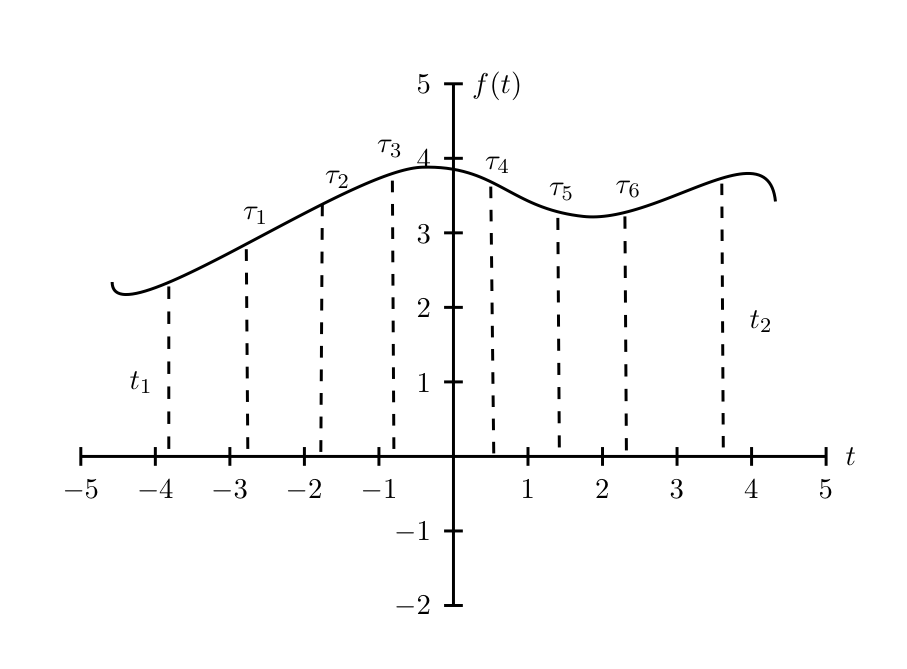
\includegraphics[scale=0.7]{Draw/function.png}
\label{}
\end{center}
\caption{Example for the integral of a function}
\label{function}
\end{figure}
Suppose that $f(t)$ represents the rate at which the size of the observable universe, $R(t)$, grows with time, that is to say $f(t)=\dot{R}(t)$; we wish to find how much the universe has expanded between $t_1$ and $t_2$, i.e. we want to calculate $R(t_2)-R(t_1)$, knowing $f(t)$ only. To do this, we must add up all the changes that $R(t)$ endures from time $t_1$ to time $t_2$: as a first approximation we break down the interval $t_2-t_1$ in several intermediate intervals $\{\tau_1,...,\tau_6\}$ and we perform the sum
\begin{equation}
R(t_2)-R(t_1)\approx f(t_1)(\tau_1-t_1)+f(\tau_1)(\tau_2-\tau_1)+...+f(\tau_6)(t_2-\tau_6)
\end{equation} 
What we are doing, basically, is approximating the area under the curve $f(t)$ enclosed by the horizontal axis and the two extremes $t_1$ and $t_2$; the above expression becomes exact when we the number of intermediate $\tau$ points that we choose becomes very large. This exact limit is called \textit{intergral} of the function $f(t)$ between $t_1$ and $t_2$ and is indicated by the notation
\begin{equation}
\int_{t_1}^{t_2}f(t)dt\equiv R(t_2)-R(t_1)
\end{equation}
This example also suggests us a statement, called \textit{fundamental theorem of calculus} that says that basically integrals and derivatives are one the inverse of the other; in fact, for \textit{any} function $R(t)$ it is true that
\begin{equation}
\int_{t_A}^{t_B}\dot{R}(t)dt=R(t_B)-R(t_A)
\end{equation}
That says that also the following is true
\begin{equation}
\frac{d}{dt}\int_{t_A}^t f(t')dt'=f(t)
\end{equation}
For \textit{any} function $f(t)$; a useful list of integrals of the most common functions can be found on \url{http://en.wikipedia.org/wiki/Lists_of_integrals}
\subsection{Differential equations}
The last concept that we need to understand before going into physical matters, is the one of \textit{differential equation}; the motivation of this is that nearly all physics is formulated in terms of statements of the kind ''we have this physical process, that causes this effect''. For example you may be already familiar with statements like ''we apply a force to a body and this causes the body to accelerate'' (the so called $F=ma$) or ''there is a temperature difference between two objects and this causes a heat flow''; you may notice that all these kinds of \textit{physical laws} can be written down in mathematical form, a form that looks like this 
\begin{equation}
\label{concept}
\mathrm{Effect(acceleration,heat \,flow)}=\mathrm{Cause(force,temperature \,difference)}
\end{equation} 
Usually the ''effect'' is the rate of change of some quantity (position, temperature,...) that involves derivatives, and the cause is some physical quantity that can depend on space and time (force for example): this is why these kind of physical laws are usually expressed in terms of \textit{differential equations} (i.e. equations that have a function as an unknown and relate the function itself to its derivatives). 
\subsubsection{Example 1}
A raindrop of mass $m$ originates from a cloud and starts falling to the ground; the forces acting on it are the usual gravity $mg$ and a frictional force that opposes to its motion. We suppose that this force is proportional to the velocity of the raindrop and write $F_{friction}=bv$ where $v$ is the vertical velocity of the raindrop. The addition of these two forces causes an acceleration, and we can write equation (\ref{concept}) as
\begin{equation}
ma=F_{gravity}-F_{friction}
\end{equation}
Or
\begin{equation}
\frac{dv(t)}{dt}=g-\frac{b}{m}v(t)
\end{equation}
We want to solve this equation for the time dependence of the velocity $v(t)$ and you can convince yourselves (looking at the derivative tables) that the solution is given by (assuming that the droplet is still at $t=0$):  
\begin{equation}
v(t)=\frac{mg}{b}(1-e^{-bt/m})
\end{equation}
\subsubsection{Example 2}
Consider a metal rod of length $L$ extending from $x=0$ to $x=L$; we keep its extremes in contact with some thermal bath so that their temperature is fixed $T(0)\equiv T_1$ and $T(L)\equiv T_2$; we want to find how the temperature of the rod changes along its length, that is to say we wish to find the function $T(x,t)$, which in general can also depend on time $t$. The physical law of heat conduction tells us that the temperature difference between points of the stick (expressed by its second derivative with respect to $x$, $\frac{\partial^2 T}{\partial x^2}$) \textit{has the effect} of causing a heat flow, expressed by the change of the temperature of the rod over time $\frac{\partial T}{\partial t}$. We may write the law of heat conduction as (take this for granted, we won't go into the details on why this is true)
\begin{equation}
\frac{\partial T(x,t)}{\partial t}=\frac{\partial^2 T(x,t)}{\partial x^2}
\end{equation} 
We seek for a \textit{stationary} solution to this equation (a solution that does not depend on time $T(x,t)=T(x)$) keeping in mind that we want to find the equilibrium profile $T(x)$; we try to solve 
\begin{equation}
\frac{d^2T(x)}{dx^2}=0
\end{equation}
Looking at the derivative table you can convince yourselves that the solution to this is given by $T(x)=ax+b$, with $a,b$ constants; for our particular problem of the rod this becomes 
\begin{equation}
T(x)=T_1+(T_2-T_1)\frac{x}{L}
\end{equation}
This completes a qualitative overview of the basic matematical instruments we need to understand (and give a justification) the most characteristic and intriguing aspects of Modern Cosmology; before going into the subject though, let us review the foundations and give a brief overview of classical physics and Newton's laws 

\section{Newton's laws}
All classical physics' phenomena (\textit{classical} means that neither quantum mechanics nor Einstein's relativity are involved in a significant way) can be described starting from these three assumptions, which were originally formulated by Isacc Newton in 17th century (backed up with the so called ''law zero'' which is an assumption on absolute space and time made by Galileo Galilei)
\begin{enumerate}
\setcounter{enumi}{-1}
\item \textit{Law zero}: there exist a special reference frame, which acts as an \textit{absolute} standard for space and time; the speed of light, $c$, is measured in this particular reference frame 
\item \textit{Law of inertia}: any physical body which experiences a \textit{zero net force} (i.e. a the sum of all forces acting on it is zero), $\mathbf{F}=0$, moves with a constant velocity $\dot{\mathbf{v}}=0$
\item \textit{Law of dynamics}: any physical body of mass $m$ that experiences a net force $\mathbf{F}$ will accelerate, with acceleration $\mathbf{a}$ given by $\mathbf{F}=m\mathbf{a}$
\item \textit{Law of action and reaction}: take two bodies labelled by $1,2$; suppose the first body exerts a force $\mathbf{F}_{12}$ on the second one. Then the second body as well exerts a force $\mathbf{F}_{21}$ on the first one, and these two forces are equal and opposite $\mathbf{F}_{21}=-\mathbf{F}_{12}$ 
\end{enumerate} 
Remember that all the quantities indicated in bold are \textit{vectors} in the sense discussed before; in order to have a taste on how these laws work, let us make some clarifying examples
\subsection{Gravity on earth's surface}
Consider an apple of mass $m$ which initially hangs from a tree at a height $z_0$ from the ground; at a certain instant ($t=0$) the apple starts to fall. We want to find how much time it will take to reach the ground; the gravitational force acting on it is $\mathbf{F}_g=-mg\hat{z}$ with $g$ being the gravitational acceleration at the earth surface, which is measured to be $g=9.81$\,m/s$^2$. Newton's second law tells us
\begin{equation}
\frac{d^2z(t)}{dt^2}=-g
\end{equation}
Which has the solution $z(t)=z_0-\frac{1}{2}gt^2$, and tells us that the apple will reach the ground in a time $T=\sqrt{\frac{2z_0}{g}}$
\subsection{Harmonic motion}
A block of mass $m$ is attached to a wall by means of a spring; we suppose that, when the block is pulled (or pushed) at a position $x$ from its equilibrium position (which corresponds to the spring rest length), it experiences a force $F=-kx$ with $k$ some constant. Let's define for convenience the \textit{angular frequency} $\omega$ as $k=m\omega^2$; again, Newton's second law tells us
\begin{equation}
\label{simpleharmonic}
\frac{d^2x(t)}{dt^2}=-\omega^2 x(t)
\end{equation}
This equation is more difficult to solve than the one in the previous problem, but the derivative tables help us again and we can find a general solution $x(t)=A\cos{\omega t}+B\sin{\omega t}$; if we let the initial conditions be $x(0)=x_0$ and $\dot{x}(0)=v(0)=v_0$ we immediately get
\begin{equation}
x(t)=x_0\cos{\omega t} + \frac{v_0}{\omega}\sin{\omega t}
\end{equation}
\subsection{Circular motion}
A little toy car of mass $m$ runs on a circular track of radius $R$ with constant speed $v$; despite the fact that the magnitude of the velocity $v$ is constant in this case, its direction is not and hence $\dot{\mathbf{v}}\neq 0$ and the car experiences acceleration and hence a net force from the track. Let's try to quantify this force; let $\hat{\mathbf{r}}$ be a unit vector that points in the car direction and $\hat{\theta}$ another unit vector that points along the car velocity, as in Figure \ref{track}; note that $\hat{\mathbf{r}}\cdot \hat{\theta}=0$. 
\begin{figure}
\begin{center}
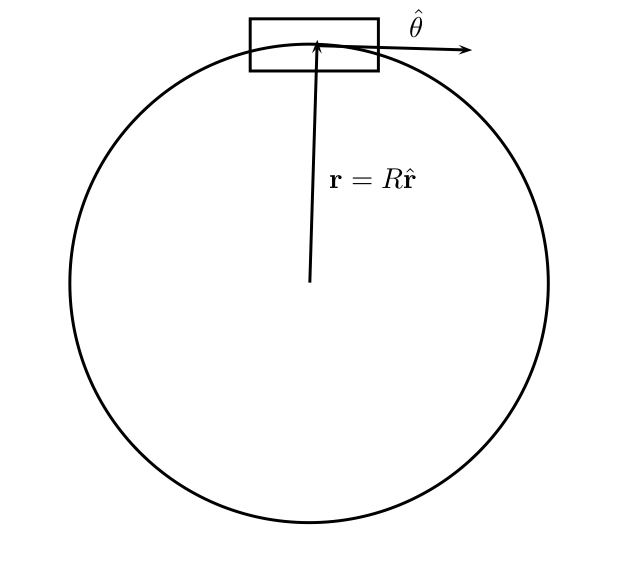
\includegraphics[scale=0.7]{Draw/circular.png}
\label{}
\end{center}
\caption{A toy car on a circular track}
\label{track}
\end{figure}
The position of the car is then described by the vector $\mathbf{r}=R\hat{\mathbf{r}}$; if we define the angular velocity of the car as $\omega=v/R$, assuming the following relations 
\begin{equation}
\frac{d}{dt}\hat{\mathbf{r}}(t)=\omega \hat{\theta}(t) \,\, ; \,\, \frac{d}{dt}\hat{\theta}(t)=-\omega \hat{\mathbf{r}}(t)
\end{equation}
We can find the acceleration of the car as
\begin{equation}
\label{centripetal}
\mathbf{a}(t)=\frac{d^2}{dt^2}\mathbf{r}(t)=R\frac{d}{dt}(\omega \hat{\theta}(t))=-\omega^2R\hat{\mathbf{r}}(t)=-a_c\hat{\mathbf{r}}(t) 
\end{equation}
Hence the car experiences an acceleration directed toward the center of the track, of magnitude $a_c=\omega^2R=v^2/R$, and hence a force directed toward the center of the track, of magnitude $F_c=m\omega^2 R=mv^2/R$.


\chapter{Special Relativity}

\section{Introduction}

The fact that light travels at a finite speed (and not instantaneously fast) has been experimentally known since the 17th century, and by the mid-19th century the numerical value of this speed had been measured with an error of less than 10$\%$. Nevertheless, the question about the precise nature of light had remained unanswered until Maxwell showed in 1861 that electromagnetic waves (oscillatory disturbances in the electric and magnetic fields) propagate in empty space at the speed of $c=3\times10^8$ m/s, precisely the measured value of the speed of light. The prediction that light is a type of electromagnetic wave (just like radio waves and microwaves) was soon verified experimentally, but with this verification new questions arised. First, how can a wave travel in empty space? After all, all the waves known to the physicists of the time were mechanical waves that propagate in materials such as liquids and gases. Second, with respect to what reference frame does light travel with the speed $c$ predicted by 
Maxwell? For if light travels with speed $c$ in some reference frame, then it better have a different speed when measured in some other reference frame that is in motion with respect to the first.\footnote{By reference frame we mean a fixed set of axes $x$, $y$ and $z$, with respect to which the positions of all the bodies in the system are measured as functions of time (it will be useful later to think of the time as another ``axis'' defining the reference frame). A reference frame is also called ``observer,'' ``reference system,'' or simply ``frame'' for short.} To make this point clear, suppose there is an observer who measures the velocity of a particle, which moves along the $x$-axis, to be $u$. Consider a second observer moving (also in the $x$-direction) with speed $v$ relative to the first. What is the speed $u'$ of the particle as measured by this second observer? Any physicist of the 19th century would have answered that
\begin{equation} \label{eq:galilean_vel_rule}
u'=u-v.
\end{equation}
This is called the Galilean velocity addition rule. Although this rule seems to rely on nothing but common sense, it actually relies on an implicit assumption regarding the nature of space and time, an assumption that turns out to be wrong as we will see.

To answer the two questions stated above the physicists of the 19th century proposed the existence of the {\it ether}, an invisible medium that permeates the whole universe. In their view, electromagnetic waves do not really travel in empty space; they are actually supported by the ether, just like sound waves are supported by the air. As for the second question, the speed $c$ predicted by Maxwell is to be measured with respect to the reference frame where the ether is at rest. If this is the case, then we should be able to measure different values of the speed of light in the winter, when the Earth is moving in one direction relative to the ether, and in the summer, when it is moving in the opposite direction. Michelson and Morley attempted to measure this difference in 1887 with completely negative results; the speed of light was measured to be $c$ in every case. Then, in 1905, Einstein came up with a radical solution: the speed of light is $c$ in every inertial reference frame. This clearly contradicts 
the Galilean velocity addition rule (for if $u=c$ then according to Einstein $u'=c$ also, regardless of the value of $v$), as well as many other results of Newtonian physics, as we will see below. This universality of the speed of light implies that the concept of the ether is completely unnecessary; there is no such thing as an absolute reference frame. This also implies that light can indeed travel in empty space; unlike mechanical waves, electromagnetic waves can propagate in vacuum.


\section{The theory of Special Relativity}

Einstein's theory of Special Relativity (SR) is based on the following two basic postulates:
\begin{itemize}
\item [\bf 1.] {\bf The principle of relativity.} The laws of physics apply in the same form in all inertial reference frames.
\item [\bf 2.] {\bf Universality of the speed of light.} The speed of light in vacuum is $c=3\times10^8$ m/s for any observer, regardless of the motion of the light's source relative to the observer.
\end{itemize}

An inertial reference frame is one in which Newton's first law holds: if you are in a frame where particles free of forces move with constant velocity, then the reference frame is inertial,\footnote{You may think that Newton's first law is nothing but a definition, since it states that isolated particles move with uniform velocity in inertial frames. But this is just how inertial frames are defined! However, how do we know that inertial frames actually exist in the first place? The statement that inertial reference frames do exist in the physical world is the true physical content of Newton's first law.} and any other frame moving with constant velocity relative to you will also be inertial. The principle of relativity then states that all these inertial frames are equivalent; there is no absolute reference frame relative to which absolute velocities can be defined.\footnote{Do not confuse the concept of absolute reference frame (like the ether) with that of {\it preferred} reference frame. Many systems of 
course have preferred frames in which its mathematical description is simple. For example, in the case of the solar system, there is a preferred coordinate system in which the Sun sits at the origin with the $z$ axis perpendicular to the plane in which the planets move.} This principle is not really modern; it was originally stated by Galileo in the context of classical mechanics, in which it is a simple consequence of Newton's second law. Indeed, consider a particle of mass $m$ moving with velocity $u(t)$ in some inertial frame (we assume motion in one dimension, say along the $x$ axis). Then Newton's second law states that the force $F$ acting on the particle is related to the velocity by the equation
\begin{equation}
F=ma=m\frac{du}{dt},
\end{equation}
where $a=du/dt$ is the acceleration of the particle. Now consider a second inertial frame moving with velocity $v$ relative to the first. By the Galilean velocity addition rule, eq.\ (\ref{eq:galilean_vel_rule}), the velocity of the particle in this second frame is $u'(t)=u(t)-v$. Notice that $u(t)$ and $u'(t)$ are functions of time (the particle's speed may be changing in time), but $v$ must be a constant for the primed frame to be also inertial. The force and the mass of the particle are (in Newtonian physics) the same in the primed frame, so Newton's second law will read
\begin{equation}
F=ma'=m\frac{du'}{dt}=m\left(\frac{du}{dt}-\frac{dv}{dt}\right)=m\frac{du}{dt},
\end{equation}
where we used that $dv/dt=0$ since $v$ is a constant. We see that Newton's second law has exactly the same form in the second inertial reference frame, consistent with the principle of relativity.

The novelty of Einstein's principle of relativity relies in its application to {\it all} of physics,\footnote{Actually, in the context of Special Relativity we should not include gravity, since it causes some troubles as we will see later. To include gravity one needs the theory of General Relativity.} not just to mechanics. It implies that no experiment of any kind can measure the absolute velocity of a body. In other words, absolute velocity is not an observable quantity, and therefore it is not a true physical concept. The second postulate is even more radical; we already remarked that it contradicts the Galilean velocity addition rule, and in the following we will see other counter-intuitive consequences of the second postulate that will show how the Newtonian notions of space and time have to be modified. But first we need a few definitions. We call an {\it event} something that happens at a single point in space at a single instant in time. An {\it observation} is the act of recording the coordinates 
$x$, $y$, $z$ of the location of an event, and the time $t$ at which the event occurs as indicated by a clock located at the point $(x,y,z)$. Two events are said to be simultaneous if the clocks at the respective locations of the events read the same time (the clocks have to be properly synchronized of course). Notice that making an observation of two simultaneous events is different from {\it seeing} two events occuring at the same instant. For example, consider two light bulbs located at $x_1=3\times10^8$ m and $x_2=6\times10^8$ m; the light bulbs are switched on at $t_1=1$ s and $t_2=0$, respectively. The event of ``first light bulb being switched on'' has the spacetime coordinates $(t_1,x_1)$,\footnote{As noted above, it is useful to think of time as just another coordinate in addition to the spatial coordinates $x$, $y$, $z$. The four dimensions $t$, $x$, $y$, and $z$ define what we call the spacetime. (We will often omit the coordinates $y$ and $z$ when talking about events that occur in one dimension.)
} and the event of ``second light bulb being switched on'' has the spacetime coordinates $(t_2,x_2)$. Since $t_1\neq t_2$ the two events are not simultaneous, although a person sitting at $x=0$ will see the two light bulbs switching on at the same time. There is no contradiction here, of course, since the person is not really observing the original two events (``light bulbs switching on''), but the different events of ``light beams reaching $x=0$'' which have coordinates $(t=2~{\rm s},x=0)$.

\subsection{The relativity of simultaneity}

Consider a train car traveling at constant speed along a straight, frictionless track (fig.\ \ref{fig:lec2_1}). At the middle point of the car there is a light bulb. The bulb is switched on at some instant, emitting two light rays in the front and back directions. Clearly, an observer on the train will find that the rays reach the front and back ends of the car at the same time, since the light bulb is equidistant from the two ends, and the rays both travel with the same speed $c$. Let us define as event $A$ when the ray reaches the front end, and as event $B$ when the other ray reaches the back end. Then, according to the observer on the train, events $A$ and $B$ are simultaneous. Now consider these same two events from the point of view of an observer on the ground. The light rays both travel with the same speed $c$ (from postulate 2), but since the train car is moving, the ray moving in the front direction will have to travel a distance larger than half of the length of the car, whereas the opposite is 
true for the ray moving in the back direction. The observer on the ground would then find that event $B$ happens before event $A$, thereby concluding that the two events are not simultaneous.
\begin{figure}[ht]
\begin{center}
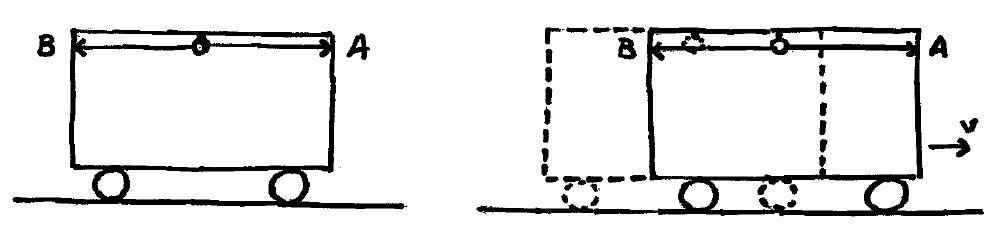
\includegraphics[scale=0.5]{Draw/lec2_1.png}
\end{center}
\caption{Relativity of simultaneity}
\label{fig:lec2_1}
\end{figure}

This example illustrates the concept of the relativity of simultaneity: two events that are simultaneous in one inertial reference frame are not, in general, simultaneous in another. It is a direct consequence of the postulate of the universality of the speed of light. Notice that, for this effect to be important, the train in the above example would have to be moving extremely fast, for otherwise the difference in the distances the two light rays must travel, as seen by the ground observer, would be extremely small. This is due to the fact that the speed of light is so much larger than any of the speeds involved in everyday life, which is why we do not easily notice this and other relativistic effects.

\subsection{Time dilation}

Consider again the train car of the previous example (which we will call system $S'$), but now suppose the light bulb sends a ray directed straight down to the floor of the car. If the height of the car is $h$, then the time it takes the light ray to reach the floor is
\begin{equation}
\Delta t'=\frac{h}{c}.
\end{equation}
\begin{figure}[ht]
\begin{center}
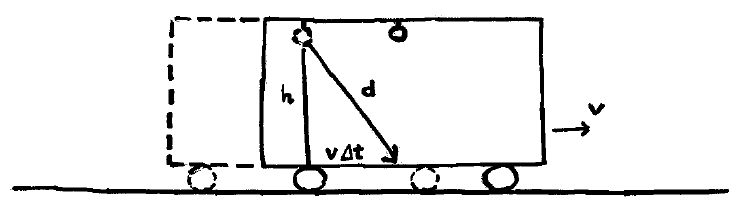
\includegraphics[scale=0.6]{Draw/lec2_2.png}
\end{center}
\caption{Time dilation}
\label{fig:lec2_2}
\end{figure}

\noindent
On the other hand, for the observer on the ground (system $S$) the light ray does not travel straight down, since the car has moved a distance $v\Delta t$ by the time the ray reaches the floor of the car. Here $\Delta t$ is the time interval as measured by the ground observer, $v$ is the speed of the train, and we have again used postulate 2 in assuming that the light ray travels with speed $c$. From fig.\ \ref{fig:lec2_2} we can see that the distance the light ray travels is given by
\begin{equation}
d=\sqrt{h^2+(v\Delta t)^2},
\end{equation}
so that the time it takes the ray to make the trip is
\begin{equation}
\Delta t=\frac{d}{c}=\frac{\sqrt{h^2+(v\Delta t)^2}}{c}.
\end{equation}
We can solve this equation for $\Delta t$, finding that
\begin{equation}
\Delta t=\frac{h}{c}\frac{1}{\sqrt{1-v^2/c^2}}.
\end{equation}
Also, since $\Delta t'=h/c$, we can write this as
\begin{equation} \label{eq:time_dilation}
\Delta t=\frac{\Delta t'}{\sqrt{1-v^2/c^2}}.
\end{equation}
Notice that $\Delta t>\Delta t'$, meaning that for the observer on the ground the time interval between the two events (``light ray being emitted,'' and ``light ray reaches the floor'') is larger than the time interval measured by the observer on the train. This is the phenomenon of time dilation, which is often summarized by the statement ``moving clocks run slow.''

\subsection{Lorentz contraction}

Once again we consider the train car traveling with speed $v$ relative to the ground. Imagine now that there is a flashlight located at the back end of the car, and a mirror at the front end, so that a light ray sent by the flashlight will make a round trip along the car (fig.\ \ref{fig:lec2_3}). For an observer on the train, the time it takes the ray to make the trip is
\begin{equation}
\Delta t'=2\frac{L_0}{c},
\end{equation}
where $L_0$ is the {\it rest length} of the train car, i.e.\ the length of the car as measured in the reference frame where it is at rest. We want to compute now this time interval as measured by an observer on the ground. Let $\Delta t_1$ be time for the light ray to reach the mirror, and $\Delta t_2$ the time to return to the back end. If the car has a length $L$ in the ground system, then the ray travels a distance $d_1=L+v\Delta t_1$ from the back to the front, since by the time it reaches the front end the train has moved a distance $v\Delta t_1$. Similarly, the light ray travels a distance $d_2=L-v\Delta t_2$ from the front to the back, since by the time the ray arrives to the back end the train has moved a distance $v\Delta t_2$ (convince yourself that this distance has to be subtracted, so that $d_2$ is shorter than $L$). The time intervals in the ground frame are therefore
\begin{equation}
\Delta t_1=\frac{L+v\Delta t_1}{c},~~~~~~~~\Delta t_2=\frac{L-v\Delta t_2}{c}.
\end{equation}
Solving for $\Delta t_1$ and $\Delta t_2$ from these equations we find
\begin{equation}
\Delta t_1=\frac{L}{c-v},~~~~~~~~\Delta t_2=\frac{L}{c+v}.
\end{equation}
\begin{figure}[ht]
\begin{center}
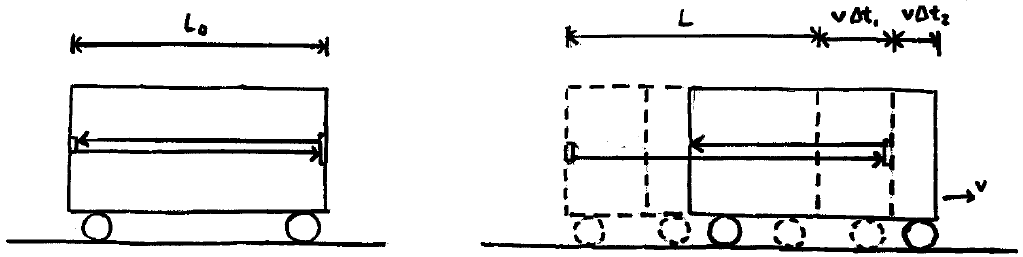
\includegraphics[scale=0.6]{Draw/lec2_3.png}
\end{center}
\caption{Lorentz contraction}
\label{fig:lec2_3}
\end{figure}

\noindent
The total time for the round trip is then
\begin{equation}
\Delta t=\Delta t_1+\Delta t_2=2\frac{L}{c}\frac{1}{(1-v^2/c^2)}.
\end{equation}
But we also know, from eq.\ (\ref{eq:time_dilation}), that the time intervals are related by $\Delta t'=\sqrt{1-v^2/c^2}\Delta t$. Applying this to the times we just found, we get
\begin{equation}
 2\frac{L_0}{c}=2\frac{L}{c}\frac{\sqrt{1-v^2/c^2}}{(1-v^2/c^2)},
\end{equation}
or
\begin{equation}
L=\sqrt{1-v^2/c^2}L_0.
\end{equation}
Notice that $L$, the length of the car observed from the ground, is shorter than $L_0$, the length of the car as measured in the frame where the car is at rest. This is the phenomenon of Lorentz contraction, which can be summarized with the sentence ``moving objects are shortened.'' It is important to note that the contraction only occurs along the direction of motion; the dimensions perpendicular to the velocity are unchanged.

\section{The Lorentz transformations}

Consider an event with coordinates $(t,x,y,z)$ in some inertial reference system $S$. We would like to find the coordinates $(t',x',y',z')$ of this same event in some other inertial system $S'$. Suppose the system $S'$ is moving with constant speed $v$ relative to the system $S$, along the positive $x$-direction. We assume that the $x$ and $x'$ axes are parallel, and that the origins $O$ and $O'$ of the two systems coincide at $t=t'=0$; see fig.\ \ref{fig:lec2_4}. Let us go back to Newtonian physics for a moment, where the time is absolute and runs at the same rate in all inertial frames. This means that $t'=t$ for the event we are considering. It is clear then, from fig.\ \ref{fig:lec2_4}, that the coordinates $(t',x',y',z')$ of the event are related to the coordinates $(t,x,y,z)$ by the equations
\begin{equation}
\begin{split}
x'&=x-vt,\\
y'&=y,\\
z'&=z,\\
t'&=t.\\
\end{split}
\end{equation}
These are called the Galilean transformations.\footnote{Notice that the Galilean velocity addition rule, eq.\ (\ref{eq:galilean_vel_rule}), follows from taking the time derivative of the first equation.} Although they seem to be quite obvious at first sight, we should not forget that we derived them from the assumption that time runs at the same rate in all inertial systems. But we now know that this is not true; we have seen how Einstein's second postulate forces us to abandon the notion of absolute time, implying that the Galilean transformations have to be modified to account for the universality of the speed of light. The correct equations read
\begin{equation} \label{eq:lorentz_transf}
\begin{split}
x'&=\gamma\left(x-vt\right),\\
y'&=y,\\
z'&=z,\\
t'&=\gamma\left(t-\frac{v}{c^2}x\right).\\
\end{split}
\end{equation}
The parameter $\gamma$ is defined as
\begin{equation}
\gamma\equiv\frac{1}{\sqrt{1-v^2/c^2}}.
\end{equation}
These are known as the Lorentz transformations. Notice that whenever $v\ll c$ (so that $\gamma\approx1$) these reduce to the Galilean transformations. This is why we can safely apply Newtonian physics as long as we deal with speeds much smaller than the speed of light.
\begin{figure}[ht]
\begin{center}
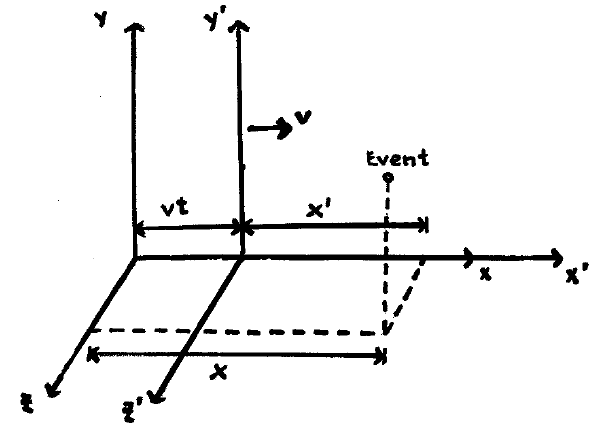
\includegraphics[scale=0.5]{Draw/lec2_4.png}
\end{center}
\caption{Galilean transformations}
\label{fig:lec2_4}
\end{figure}

Next consider two events separated in space by the distances $(\Delta x,\Delta y,\Delta z)$ and in time by the interval $\Delta t$, as measured in the system $S$. For definiteness, we can think of the two events as ``a particle located at the spacetime point $(t,x,y,z)$'' and ``the same particle located at the spacetime point $(t+\Delta t,x+\Delta x,y+\Delta y,z+\Delta z)$,'' so that we keep track of the particle's motion by means of two events. Now we can apply the Lorentz transformations to these two events and find their coordinates in the system $S'$. One can then show that, by subtracting the equations for the two events, the intervals $\Delta t'$, $\Delta x'$, $\Delta y'$, and $\Delta z'$ measured in the frame $S'$ are given by
\begin{equation} \label{eq:lorentz_intervals}
\begin{split}
\Delta x'&=\gamma\left(\Delta x-v\Delta t\right),\\
\Delta y'&=\Delta y,\\
\Delta z'&=\Delta z,\\
\Delta t'&=\gamma\left(\Delta t-\frac{v}{c^2}\Delta x\right).\\
\end{split}
\end{equation}
Suppose the particle is moving in the $x$-direction, so that $\Delta y=\Delta y'=0$ and $\Delta z=\Delta z'=0$. We can compute the ratio $\Delta x'/\Delta  t'$ from these equations as follows:
\begin{equation}
\frac{\Delta x'}{\Delta t'}=\frac{\gamma\left(\Delta x-v\Delta t\right)}{\gamma\left(\Delta t-\frac{v}{c^2}\Delta x\right)}=\frac{\frac{\Delta x}{\Delta t}-v}{1-\frac{v}{c^2}\frac{\Delta x}{\Delta t}}.
\end{equation}
But $\Delta x/\Delta t\equiv u$ is equal to the velocity of the particle in the system $S$, whereas $\Delta x'/\Delta t'\equiv u'$ is its velocity in the system $S'$. The above equation then tells us how to relate $u$ and $u'$:
\begin{equation} \label{eq:einstein_vel_rule}
u'=\frac{u-v}{1-\frac{vu}{c^2}}.
\end{equation}
This is known as Einstein's velocity addition rule, which is the analog of the Galilean rule in SR. Note that if $u\ll c$ and $v\ll c$ Einstein's rule reduces to the Galilean rule, as it should. To check that this formula is consistent with the universality of the speed of light, suppose the particle is a photon, so that $u=c$ in the system $S$. Then its speed in the system $S'$ is
\begin{equation}
u'=\frac{c-v}{1-\frac{v}{c}}=c,
\end{equation}
so that indeed the photon has a speed $c$ in all reference frames.

\par\vspace{\baselineskip}

{\bf Exercise.} Derive the formulas for time dilation and Lorentz contraction starting from the Lorentz transformations.

\section{The spacetime interval}

Given two events separated in spacetime by $(\Delta t,\Delta x,\Delta y,\Delta z)$, as measured in some inertial reference system $S$, we define the {\it spacetime interval} between the events as
\begin{equation}
\Delta s^2=-c^2\Delta t^2+\Delta x^2+\Delta y^2+\Delta z^2.
\end{equation}
We would like to know how does this spacetime interval change when we consider the same two events in a reference frame $S'$ that moves with velocity $v$ relative to $S$ in the $x$-direction (with the respective axes parallel, just as in the previous section). To answer this we simply have to compute the interval $\Delta s'^2$ using the Lorentz transformations of eq.\ (\ref{eq:lorentz_intervals}):
\begin{equation}
\begin{split}
\Delta s'^2&=-c^2\Delta t'^2+\Delta x'^2+\Delta y'^2+\Delta z'^2\\
&=-c^2\left[\gamma\left(\Delta t-\frac{v}{c^2}\Delta x\right)\right]^2+\left[\gamma\left(\Delta x-v\Delta t\right)\right]^2+\Delta y^2+\Delta z^2\\
&=\Delta t^2\left[-\gamma^2c^2+\gamma^2v^2\right]+\Delta x^2\left[-\gamma^2\frac{v^2}{c^2}+\gamma^2\right]+\Delta x\Delta t\left[2c^2\gamma\frac{v}{c^2}-2\gamma v\right]+\Delta y^2+\Delta z^2\\
&=-c^2\Delta t^2+\Delta x^2+\Delta y^2+\Delta z^2.
\end{split}
\end{equation}
Thus we have obtained the very important result
\begin{equation}
\Delta s'^2=\Delta s^2,
\end{equation}
which states that the spacetime interval between two events has the same value in all inertial reference frames. We say that $\Delta s^2$ is {\it invariant} under Lorentz transformations. In the modern point of view, the invariance of the interval is often taken as the starting point of SR.\footnote{We showed that $\Delta s^2$ is invariant by using the Lorentz transformations, but it turns out that one can also do the opposite, that is, to derive the Lorentz transformations starting from the invariance of the interval.} The reason for this is that, as we will see later, the interval allows us to understand spacetime in a geometrical way, which will be useful when we move on to study General Relativity. To see how to use the interval in practice, we will now rederive the formulas of time dilation and Lorentz contraction by exploiting the invariance of $\Delta s^2$.

\subsection{Time dilation again}

Consider a train (system $S'$) moving with speed $v$ relative to the platform (system $S$), as shown in fig.\ \ref{fig:lec2_5}. There is a clock traveling on the train, and we want to find the time elapsed between two successive ticks as measured in $S$ and in $S'$. We do this by computing the spacetime interval between the two events (first tick and second tick) in the respective reference systems.
\begin{figure}[ht]
\begin{center}
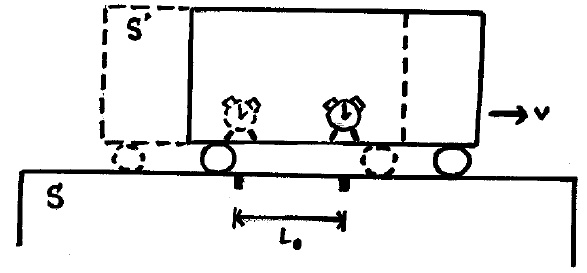
\includegraphics[scale=0.6]{Draw/lec2_5.png}
\end{center}
\caption{The spacetime interval}
\label{fig:lec2_5}
\end{figure}

For an observer on the train $\Delta x'=0$, since from his point of view the two ticks occur at the same place. Therefore the interval in the system $S'$ is simply
\begin{equation}
\Delta s'^2=-c^2\Delta t'^2.
\end{equation}
For an observer on the platform the clock is moving with speed $v$, so for her the second tick will take place at a distance $v\Delta t$ from the location of the first tick, i.e.\ $\Delta x=v\Delta t$. The interval in the system $S$ is then
\begin{equation}
\begin{split}
\Delta s^2&=-c^2\Delta t^2+(v\Delta t)^2\\
&=-c^2\Delta t^2\left(1-\frac{v^2}{c^2}\right).
\end{split}
\end{equation}
Next we use the fact that $\Delta s'^2=\Delta s^2$, which implies that
\begin{equation}
-c^2\Delta t^2\left(1-\frac{v^2}{c^2}\right)=-c^2\Delta t'^2
\end{equation}
\begin{equation}
\Rightarrow~~~~\Delta t=\frac{\Delta t'}{\sqrt{1-v^2/c^2}},
\end{equation}
which is the time dilation formula we found above.

\subsection{Lorentz contraction again}

Let us repeat the experiment we just described, but this time we ask the observer on the platform (system $S$) to make two marks on the platform edge at the positions where the clock traveling on the train (system $S'$) makes the two ticks. She measures the distance between the two marks to be $L_0$. Clearly, if the train is moving with speed $v$ and the time elapsed between the ticks is $\Delta t$, then $L_0=\Delta x=v\Delta t$ (recall that the clock's ticks are the events we are focusing on). The spacetime interval in system $S$ is then
\begin{equation}
\begin{split}
\Delta s^2&=-c^2\Delta t^2+\Delta x^2\\
&=-c^2\left(\frac{L_0}{v}\right)^2+L_0^2\\
&=-c^2L_0^2\left(\frac{1}{v^2}-\frac{1}{c^2}\right).\\
\end{split}
\end{equation}
Next we analize the experiment from the point of view of the obsever on the train. He sees the platform moving with speed $v$ in the opposite direction, and so he will conclude that the distance between the marks on the plarform is $L=v\Delta t'$, where $\Delta t'$ is the time separating the ticks as measured on the frame of the train. Also, in this system the two ticks occur at the same place (the clock is not moving relative to the train), so that $\Delta x'=0$. Thus the spacetime interval in system $S'$ is simply
\begin{equation}
\begin{split}
\Delta s'^2&=-c^2\Delta t'^2+\Delta x'^2\\
&=-c^2\frac{L^2}{v^2}.
\end{split}
\end{equation}
Finally, since the interval is invariant we can equate $\Delta s^2$ and $\Delta s'^2$, finding that
\begin{equation}
-c^2L_0^2\left(\frac{1}{v^2}-\frac{1}{c^2}\right)=-c^2\frac{L^2}{v^2}
\end{equation}
\begin{equation}
\Rightarrow~~~~L=\sqrt{1-v^2/c^2}L_0,
\end{equation}
and we recover the Lorentz contraction formula.

\section{Relativistic momentum and energy}

In Newtonian physics two very important quantities are the momentum and the energy. For a particle of mass $m$ moving with velocity $\mathbf{v}$, the momentum is defined as
\begin{equation}
\mathbf{p}=m\mathbf{v}, 
\end{equation}
and its energy is defined as
\begin{equation}
E=\frac{1}{2}mv^2+V,
\end{equation}
where the first term on the right is the kinetic energy, and $V$ is the potential energy. Here $v=|\mathbf{v}|$ is the norm of the velocity vector, also called the speed. The momentum and energy of a system of several particles are simply given by the sum of the momenta and energies of the individual particles, respectively. The reason why these two definitions are useful is that momentum and energy satisfy {\it conservation laws}. The law of conservation of momentum states that when a component of the net force acting on a system is zero, then the corresponding component of the momentum of the system is constant in time. The law of conservation of energy states that the total energy of an isolated system remains constant in time.

A natural question to ask is whether similar conservation laws exist in SR. It is not hard to see that we cannot define momentum and energy as in Newtonian physics and expect them to satisfy conservation laws. For instance, suppose we stubbornly go ahead and define the momentum of a particle as $\mathbf{p}=m\mathbf{v}$, and postulate that this quantity must satisfy a conservation law (of course, any modern experiment in particle physics would rule out such a postulate; but let us put ourselves in the shoes of the physicists of the early 20th century). Consider the collision of two particles with masses $m_1$ and $m_2$ that move along the $x$ axis in some inertial frame $S$. The particles have velocities $u_{1i}$ and $u_{2i}$ before the collision, and velocities $u_{1f}$ and $u_{2f}$ after the collision. Our (wrong) conservation law would then imply that
\begin{equation}
m_1u_{1i}+m_2u_{2i}=m_1u_{1f}+m_2u_{2f}.
\end{equation}
We want the conservation law to be consistent with SR. Consider the collision as seen in an inertial frame $S'$ moving with velocity $v$ relative to the the system $S$. The first postulate of SR says that if momentum is conserved in $S$, then it must also be conserved in $S'$. We also know, from the second postulate, that velocities transform according to Einstein's velocity addition rule (\ref{eq:einstein_vel_rule}) when going from one inertial frame to another. Thus we can calculate the total Newtonian momentum of the particles before and after the collision as measured in the system $S'$:
\begin{equation}
m_1u_{1i}'+m_2u_{2i}'=m_1\frac{u_{1i}-v}{1-u_{1i}v/c^2}+m_2\frac{u_{2i}-v}{1-u_{2i}v/c^2},
\end{equation}
\begin{equation}
m_1u_{1f}'+m_2u_{2f}'=m_1\frac{u_{1f}-v}{1-u_{1f}v/c^2}+m_2\frac{u_{2f}-v}{1-u_{2f}v/c^2}.
\end{equation}
You should convince yourself that the right hand sides of these two equations are {\it not} equal to each other, meaning that the Newtonian momentum is not conserved in the system $S'$, thereby violating the principle of relativity. (It is important to note that the masses of the particles are the same in the two reference frames; this is because the mass of a particle is an intrinsic property which cannot depend on the particular choice of frame.)

\par\vspace{\baselineskip}

{\bf Exercise.} Repeat the above calculation using the Galilean velocity addition rule (eq.\ (\ref{eq:galilean_vel_rule})) instead of Einstein's rule. Show that in this case the Newtonian momentum is conserved in the system $S'$ if it is conserved in the system $S$. This result should not be surprising of course; it simply says that the Galilean velocity addition rule is consistent with the principle of relativity as applied to Newtonian physics.

\par\vspace{\baselineskip}

The correct relativistic expression for the momentum of a particle of mass $m$ and velocity $\mathbf{v}$ is
\begin{equation} \label{eq:rel_momentum}
\mathbf{p}=\gamma m\mathbf{v}=\frac{m\mathbf{v}}{\sqrt{1-v^2/c^2}},
\end{equation}
where we used the definition of the parameter $\gamma$. Note that when the velocity is much smaller than the speed of light (so that $\gamma\approx1$) this formula reduces to the usual Newtonian momentum.

The relativistic energy on the other hand is given by
\begin{equation} \label{eq:rel_energy}
E=\gamma mc^2=\frac{mc^2}{\sqrt{1-v^2/c^2}}.
\end{equation}
(Here and in the following we will consider free particles; in the case of particles subject to an external force we would simply add a potential energy to the above expression.) In the case when the particle is not moving ($v=0$), we get the famous expression for the rest energy of a particle of mass $m$:
\begin{equation}
E_{\rm rest}=mc^2.
\end{equation}
Also, if the velocity of the particle is small compared to the speed of light, we have
\begin{equation}
\gamma\approx 1+\frac{v^2}{2c^2}
\end{equation}
(try to show this if you know about Taylor's theorem), which gives the following approximation for the energy:
\begin{equation}
E\approx mc^2+\frac{1}{2}mv^2.
\end{equation}
We recognize the second term on the right as the Newtonian kinetic energy. But what about the rest energy? For a slowly moving particle the rest energy is much larger than the kinetic energy, so you may ask how is it that nobody observed it until the 20th century. The answer is that in nonrelativistic processes the rest energy never changes. This means that for any such process $E_{\rm rest}$ before equals $E_{\rm rest}$ after. The rest energy would then cancel in the equation of conservation of energy, so we could agree to simply ignore it from the beginning. It is only in relativistic processes, where the masses of the particles involved can change, that it becomes crucial to take the rest energy into account.

Now that we have the correct relativistic expression for the momentum, we could repeat the calculation we did at the beginning of this section, and try to show that if the total momentum is conserved in the system $S$ then it is also conserved in the system $S'$. It turns out that this is true {\it if} the relativistic energy is also conserved. Notice that this is in contrast to the situation in Newtonian physics, where energy and momentum are {\it separately} conserved. Heuristically, the reason for this is that when going from one inertial frame to another the time and space dimensions ``get mixed'' (as seen in the Lorentz transformations). You can think of the energy as the momentum in the time direction (this statement is more than a mere analogy, and can be made more precise), which means that if the time and space dimensions get mixed, then so do the energy and momentum. The bottomline is that in SR momentum is conserved if energy is also conserved, and vice versa (where by ``conserved'' we mean that 
it satisfies a conservation law consistent with the principle of relativity).

A very important relation between energy and momentum can be found by eliminating the velocity from eqs.\ (\ref{eq:rel_momentum}) and (\ref{eq:rel_energy}). First, take the norm of the momentum and divide by the energy to get
\begin{equation} \label{eq:rel_velocity}
v=\frac{pc^2}{E},
\end{equation}
where $v=|\mathbf{v}|$ and $p=|\mathbf{p}|$. Plugging this into the formula for the energy and rearranging we obtain
\begin{equation}
E^2=p^2c^2+m^2c^4.
\end{equation}
An important consequence of this relation is that it provides an expression for the momentum of a photon (for which $m=0$) in terms of the energy:
\begin{equation}
p_{\rm photon}=\frac{E_{\rm photon}}{c}=\frac{h\nu}{c},
\end{equation}
where we used that the energy of a photon is given by $E_{\rm photon}=h\nu$, with $\nu$ being its frequency and $h$ the Planck constant. Notice that if we use this relation in eq.\ (\ref{eq:rel_velocity}) we find
\begin{equation}
v_{\rm photon}=c,
\end{equation}
consistent with the fact that light is ``composed'' of photons (we will make this statement more precise when we study a little bit of particle physics later in the course).

\section{The metric tensor}

The fact that the Lorentz transformations mix the time with the spatial coordinates implies that we can no longer think of time and space as being separate entities. Rather, we should think of $t$, $x$, $y$, and $z$ as the coordinates of a 4-dimensional spacetime. The goal of this section is to understand the spacetime of SR (also known as flat spacetime or the Minkowski spacetime) in a geometrical way. This will be crucial for our study of General Relativity, which can be thought of as the generalization of SR to curved spacetimes (the concept of curvature will be explained later). We will develop the necessary mathematical tools by first studying the familiar case of Euclidean space.

First we need to introduce the concept of differential. Consider a distance or length $\Delta x$ along the $x$ axis. It is useful sometimes to think of $\Delta x$ as being infinitesimal (i.e., arbitrarily small, smaller than any length you can think of), in which case we write $\Delta x=dx$, where $dx$ is the differential of the coordinate $x$. Similarly, $dy$ and $dz$ are the differentials of the coordinates $y$ and $z$, respectively. (If you have studied calculus, you probably know that differentials are related to derivatives.)

\subsection{Euclidean space}

Given two points on the plane with coordinates $(x,y)$ and $(x+dx,y+dy)$, we know very well from the Pythagorean theorem that the distance $ds$ between them is given by $ds^2=dx^2+dy^2$ (fig.\ \ref{fig:lec2_6}). If we now consider two points living in 3-dimensional space rather than in the 2-dimensional plane, with coordinates $(x,y,z)$ and $(x+dx,y+dy,z+dz)$, then the distance $ds$ between them satisfies
\begin{equation} \label{eq:euclid_line_elem}
ds^2=dx^2+dy^2+dz^2.
\end{equation}
In elementary (old) geometry one can deduce eq.\ (\ref{eq:euclid_line_elem}) starting from Euclid's axioms. In differential (modern) geometry, however, one takes eq.\ (\ref{eq:euclid_line_elem}) as the starting point, from which one can derive all the geometrical properties of space. This is the point of view we will take from now on, since it provides the tools for studying the more general spaces we will encounter in General Relativity.

\par\vspace{\baselineskip}

{\bf Exercise.} Prove equation (\ref{eq:euclid_line_elem}) using the 2-dimensional Pythagorean theorem.

\par\vspace{\baselineskip}
\begin{figure}[ht]
\begin{center}
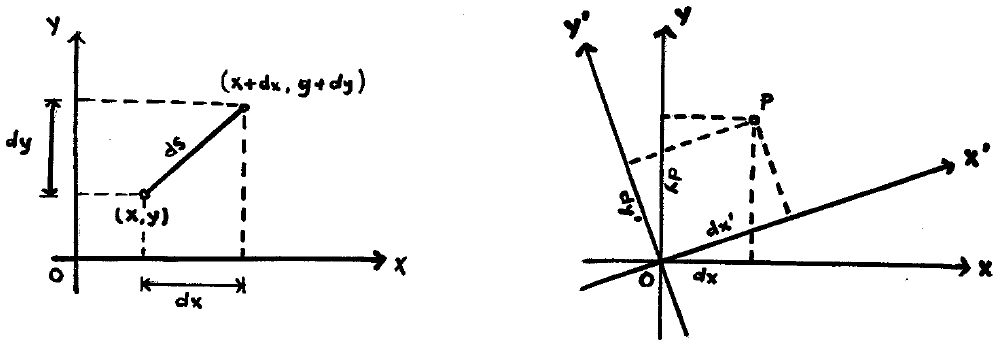
\includegraphics[scale=0.6]{Draw/lec2_6.png}
\end{center}
\caption{Euclidean space}
\label{fig:lec2_6}
\end{figure}

Next we introduce some useful notation. We write the coordinates $x$, $y$, $z$ as $x^i$, where the index $i=1,2,3$. In other words, we define
\begin{equation}
\begin{split}
x^1&\equiv x,\\
x^2&\equiv y,\\
x^3&\equiv z.
\end{split}
\end{equation}
Remember, the $i$ on $x^i$ is simply an index, not a power. The reason for writing it as an upper index will become clear later. We will also denote as $\delta_{ij}$ the components of the $3\times3$ identity matrix:
\begin{equation}
I=\left( \begin{array}{ccc} 1 & 0 & 0 \\ 
0 & 1 & 0 \\
0 & 0 & 1 \end{array} \right)
\end{equation}
The index $i$ on $\delta_{ij}$ denotes de row, and the index $j$ denotes de column. For example, $\delta_{21}$ represents the entry on the 2nd row and 1st column of $I$, which we see is zero. Clearly we have
\begin{equation}
\delta_{ij}=\begin{cases} 1, & \mbox{if $i=j$} \\ 
0, & \mbox{if $i\neq j$} \end{cases}
\end{equation}
Let us now multiply $\delta_{ij}$ with $dx^i dx^j$ and sum over all values of $i$ and $j$:
\begin{equation}
\begin{split}
\sum_{i=1}^3\sum_{j=1}^3 \delta_{ij}dx^i dx^j &= \delta_{11}(dx^1)^2+\delta_{22}(dx^2)^2+\delta_{33}(dx^3)^2\\
&= dx^2+dy^2+dz^2,
\end{split}
\end{equation}
which is precisely the right hand side of eq.\ (\ref{eq:euclid_line_elem}). We will simplify the notation by introducing now the {\it Einstein summation convention} (see also Chapter 1): whenever an expression contains one index as a superscript and the {\it same} index as a subscript, a summation is implied over all values the index can take. With this convention we can then write
\begin{equation} \label{eq:euclidean_metric}
ds^2=\delta_{ij}dx^i dx^j.
\end{equation}
The space where distances are measured using eq.\ (\ref{eq:euclidean_metric}) is called Euclidean space. The tensor $\delta_{ij}$ is called the {\it metric} of Euclidean space.

\par\vspace{\baselineskip}

{\bf Exercise.} Here is an exercise so that you start getting used to the Einstein summation convention. Let $M_{ij}$ be the components of the matrix
\begin{equation}
M=\left( \begin{array}{ccc} 1 & 2 & -1 \\ 
3 & 0 & -2 \\
2 & 4 & 1 \end{array} \right),
\end{equation}
let $a^i$ be the components of the vector $\mathbf{a}=(2,-1,0)$, and let $b^i$ be the components of the vector $\mathbf{b}=(-1,0,-2)$. Show that $M_{ij}a^ib^j=1$.

\par\vspace{\baselineskip}

An obvious but important property of $ds^2$ is that it is invariant under coordinate transformations. This is very intuitive: the distance between two points in space cannot depend on how we set up the $x$, $y$ and $z$ axes. We could even choose a different set of coordinates, for instance spherical coordinates, and the distance should obviously not change. In the example of fig.\ \ref{fig:lec2_6} we have rotated the $x$ and $y$ axes into the $x'$ and $y'$ axes (we are in 2 dimensions now). The distance $ds$ from the origin $O$ to the point $P$ has components $dx$ and $dy$ along the $x$ and $y$ axes, and components $dx'$ and $dy'$ along the $x'$ and $y'$ axes. Note that $dx\neq dx'$ and $dy\neq dy'$, but $dx^2+dy^2=dx'^2+dy'^2$, meaning that $ds^2$ is the same in both coordinate systems.

\subsection{Minkowski spacetime}

How do we measure ``distances'' in spacetime? We would like to define some sort of distance between two events (i.e.\ two points in spacetime) that is independent of the reference frame, just like the Euclidean distance is independent of the orientation of axes. We already know the answer: we have seen above that the spacetime interval $\Delta s^2$ between two events remains invariant when going from one inertial frame to another. Taking $\Delta s$ to be infinitesimal we can write down the spacetime interval in terms of differentials as
\begin{equation}
ds^2=-c^2dt^2+dx^2+dy^2+dz^2.
\end{equation}
Next we simplify the notation as we did in the case of 3 dimensions. We use the same notation for the spatial coordinates, and introduce the coordinate $x^0=ct$. In summary, the 4 coordinates we will use to describe spacetimes will be then
\begin{equation}
\begin{split}
x^0&\equiv ct,\\
x^1&\equiv x,\\
x^2&\equiv y,\\
x^3&\equiv z.
\end{split}
\end{equation}
Define the matrix
\begin{equation}
\label{etamunu}
\eta=\left( \begin{array}{cccc} -1 & 0 & 0 & 0 \\ 
0 & 1 & 0 & 0 \\
0 & 0 & 1 & 0 \\
0 & 0 & 0 & 1\end{array} \right).
\end{equation}
The components of this matrix are denoted by $\eta_{\mu\nu}$, where the indices $\mu$ and $\nu$ range from $0$ to $3$. (The convention is that latin indices are restricted to the spatial coordinates, so they range from 1 to 3, whereas greek indices are used for spacetime coordinates, so they also include the time or zeroth component.) If we multiply $\eta_{\mu\nu}$ by $dx^{\mu}dx^{\nu}$ and sum over all values of $\mu$ and $\nu$, we get
\begin{equation}
\begin{split}
\eta_{\mu\nu}dx^{\mu}dx^{\nu}&\equiv \sum_{\mu=0}^3\sum_{\nu=0}^3 \eta_{\mu\nu}dx^{\mu}dx^{\nu}\\
&=\eta_{00}(dx^0)^2+\eta_{11}(dx^1)^2+\eta_{22}(dx^2)^2+\eta_{33}(dx^3)^2\\
&=-c^2dt^2+dx^2+dy^2+dz^2,
\end{split}
\end{equation}
which is precisely equal to the spacetime interval. We conclude that
\begin{equation} \label{eq:mink_metric}
ds^2=\eta_{\mu\nu}dx^{\mu}dx^{\nu}.
\end{equation}
The spacetime where intervals between events are measured using eq.\ (\ref{eq:mink_metric}) is called Minkowski spacetime. The tensor $\eta_{\mu\nu}$ is called the metric of Minkowski spacetime.

Just as the squared distance $ds^2$ of Euclidean space is invariant under rotations of the coordinate axes, so the interval $ds^2$ of Minkowski spacetime is invariant under Lorentz transformations. Actually, the invariance of $ds^2$ is a stronger statement. In Euclidean space $ds^2$ is not only invariant under rotations of axes, but also under a general coordinate transformation. The difference is that, whereas in the case of a rotation of axes the metric $\delta_{ij}$ does not change,\footnote{We saw in the example of fig.\ \ref{fig:lec2_6} that $ds^2=dx^2+dy^2=dx'^2+dy'^2$, which can be written as $ds^2=\delta_{ij}dx^idx^j=\delta_{ij}dx'^idx'^j$ (with $dz=dz'=0$ in 2 dimensions). In other words, the metric is the same in the two coordinate systems, namely $\delta_{ij}$.} in the general case the metric will change when going from one coordinate system to another. Similarly, in Minkowski spacetime the metric $\eta_{\mu\nu}$ does not change when going from one inertial frame to another, since inertial frames 
are always connected by Lorentz transformations, but it will change if we go to more general reference frames, such as accelerated frames. As we will see in the next lecture, Einstein noted the equivalence between an accelerated frame and a frame subject to a gravitational field. This observation led him to establish a deep connection between the metric of spacetime and the gravitational field, which is the basis of General Relativity.


\chapter{General relativity and Gravity}

In the previous chapter we learned how Newton's laws and the concepts of space and time themselves are to be rethinked of when we want to study nature at speeds close to the speed of light. Einstein Special Relativity has proven to be succesful in describing a huge variety of phenomena, from time dilations and length contractions to collision of particles and the propagation of electromagnetic waves in vacuum and through matter. The one thing that it fails in explaining, though, and that we will need to understand in order to study Modern Cosmology, is gravity. In this chapter we will first give an overview on how gravity is thought about classically (as Newton did), then explaining why this picture is in contradiction with Special Relativity, and finally how Einstein solved the problem with his formulation of General Relativity.

\section{Newton's gravity}
The main reason that led Isacc Newton in formulating his theory of gravity in the 16$^{\mathrm{th}}$ century, was that at the time there was a pretty solid empirical understanding of the motion of celestial bodies (planets); at the time the astronomer Johannes Kepler inferred from his observations three empirical rules that seemed to describe very well the orbital motion of the planets in the solar system
\begin{enumerate}
\item \textit{First rule}: the planets move in elliptical orbits around the sun; the sun coincides with one of the focal points of the orbit
\item \textit{Second rule}: the vector that connects the sun and the planet, $\mathbf{r}$, swipes equal areas in equal amounts of time
\item \textit{Third rule}: the square of the orbital period $T$ is proportional to the cube of the semimajor axis of the orbit $a$, namely $T^2=ka^3$ with $k$ a suitable proportionality constant
\end{enumerate}
\begin{figure}
\begin{center}
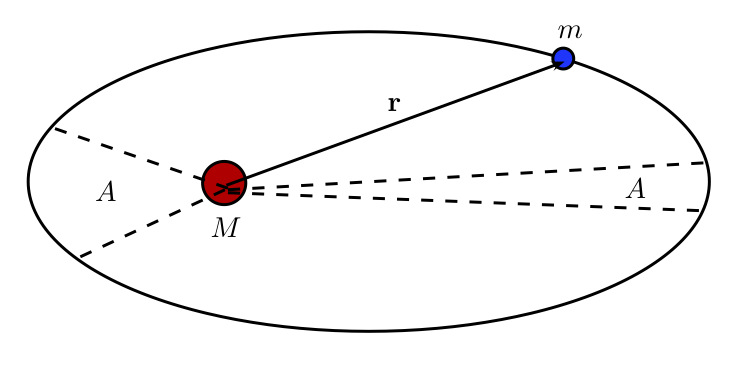
\includegraphics[scale=0.7]{Draw/kepler.png}
\label{}
\end{center}
\caption{Schematic representation of a planet's orbit: the gravitational force is always directed along the line that joins the planet and the sun; for this reason angular momentum is conserved and if the two arcs highligthened by dashed lines are covered in equal time intervals, than also the swiped areas, $A$, are the same}
\label{kepler}
\end{figure}
Newton formulated his theory of gravity with these three rules in mind as a guidance; what he came up with is that gravity is an attractive force between two bodies, it's always directed along the line that joins the objects and it's directly proportional to the product of their masses and inversely proportional to the square of their distance. With the reference of Figure \ref{kepler}, the planet, of mass $m$, according to Newton, feels an attractive force $\mathbf{F}_g$ from the sun, of mass $M$ given by
\begin{equation}
\label{newtgrav}
\mathbf{F}_g=-\frac{GmM}{r^2}\hat{\mathbf{r}}
\end{equation} 
Where the $G$ is a universal constant (Newton's constant) that was first measured by Cavendish in 1797 to be $G=6.67\times 10^{-11}\,\mathrm{m}^3\mathrm{kg}^{-1}\mathrm{s}^{-2}$; roughly speaking, Newton figured out that if rule 2 had to be satisfied then the orbital angular momentum of the planet had to be conserved during the orbit. This means that the gravitational force needs to be \textit{central} (i.e. directed along the line that connects the two bodies); the fact that orbits were closed ellipses with the force center in one of the focal points told him that only a $1/r^2$ dependence would do the trick (this is complicated to show, but you can take for granted that a $1/r^n$ dependence doesn't give closed orbits in general). Once established this, the third rule follows as a consequence of equation (\ref{newtgrav}): one can show that the proportionality constant $k$ depends only on the mass of the sun $k=\frac{4\pi^2}{GM}$. This theory of gravity explains basically all the solar system physics (except 
the orbit of mercury), from whose observations it was deduced; this has nevertheless some flaws. First of all, it violates special relativity; as if this wasn't enough, modern astronomical techiques pointed out the existence of several astrophysical systems for which a description in terms of newtonian gravity fails. We shall explore these concepts in the following paragraph. 

\section{The need for a new description}
In this paragraph we will try to understand the main flaws of Newton's gravity and why do we need a new description to understand the physics of the universe at its largest scales. As a first impression, you may notice that there is already a problem with equation (\ref{newtgrav}), in which the speed of light $c$ doesn't appear explicitely. Since in all relativity the speed of light plays a crucial role, the fact that this is not included in Newton's formulation already tells us that there will be some problems in conciliating the two pictures. Equation (\ref{newtgrav}) has however a worse problem: what it implies, in fact, is that gravity travels at infinite speed and any changes that occur on the sun are instantaneously reflected on all the surrounding planets (this is the so called \textit{action at a distance} problem). Since Einstein tells us (and there is also very solid experimental evidence) that no signal can travel faster than the speed of light, this is in explicit violation with relativity. For 
example, if our sun, which is 8 light minutes away from us, had to blow apart, earth wouldn't feel any effect until 8 minutes from the explosion at best. This feature is not captured by equation (\ref{newtgrav}). 
\subsection{The breakdown limit}
We can give some rough estimates on which is the limit above which Newtonian gravity is not reliable anymore; these estimates have to involve the speed of light, which is not included in the newtonian description. Consider a compact object (a planet, a star,...) of mass $M$ and radius $R$; using equations (\ref{centripetal}) and (\ref{newtgrav}) we can try to calculate the orbital speed $v$ for a circular orbit of radius $\gtrsim R$ using $\frac{v^2}{R}=\frac{GM}{R^2}$ which gives us $v=\sqrt{\frac{GM}{R}}$. This velocity scale is not very meaningful, what is meaningful though is the quantity $v_f=v\sqrt{2}$ which is the \textit{escape speed} from the object's surface: this is the minumum speed you need to give a rocket for it to escape the gravitational pull of the object. If the object were earth, for example, the escape speed from its surface would be $v_f=11.6$\,km/s; what if the object is much more compact and the escape velocity from it approaches $c$? This is precisely when newtonian gravity breaks 
down: a compact object so massive that $v_f=c$ is called a \textit{black hole} and it cannot be described in any way by newtonian gravity. $v_f=c$ is equivalent to say
\begin{equation}
\label{stronggrav}
\frac{GM}{Rc^2}=\frac{1}{2}
\end{equation} 
This will be our thumb rule for estimating when newton gravity breaks down: each time we have a system of mass $M$ and typical size $L$, we compute the ratio $\frac{GM}{Lc^2}$: if this ratio is much less than one ($v_f\ll c$) than we are fine, otherwise we need to come up with a better description of gravity. Let's give a few examples to have an idea on when this is the case
\begin{table}[htdp]
\begin{center}
\begin{tabular}{|c|c|c|c|} \hline
\textbf{System} & \textbf{Mass}($M$) & \textbf{Size}($L$) & \textbf{Ratio} $GM/Lc^2$ \\ \hline
The sun & $M_\odot\approx 2\cdot 10^{30}$\,kg & $7\cdot10^5$\,km &$10^{-5}$ \\ \hline
A typical neutron star & $M_\odot$ & 10\,km &1/3 \\ \hline
The universe (density $\rho \approx 10^{-30}\mathrm{g}\,\mathrm{cm}^{-3}$)& $\rho d_H^3$ & $d_H=H_0/c$ &$G\rho/H_0^2\approx 0.1\div0.5$ \\ \hline

\end{tabular}
\end{center}
\caption{A few estimates for newtonian gravity validity}
\end{table}
And we see that, even if for the sun Newton's gravity is perfectly acceptable as a description, when we move to more dense objects like neutron stars we really need to look for a better model. This is true also for the universe: if we want to study it at its largest observable scales and understand its key properties, newtonian gravity is not reliable. Before exploring the solution to this problem (which is Einstein general relativity), let's appreciate the fact that even if it works very well, newtonian gravity has some little flaws also in the solar system: for example, it fails in predicting some key features in Mercury's orbit. Mercury is the closest solar system planet to the sun and hence it's the one on which general relativistic effects are expected to be bigger; observationally Mercury's orbit exibits a very curious phenomenon, which is called \textit{perihelion precession}. Since for the gravitational force Mercury experiences from the sun is not exactly $\propto 1/r^2$, but it gets some non 
negligible general relativistic corrections $\propto 1/r^4$, its orbit is not exactly an ellipse, but it's an ellipse which perihelion (closest point of approach to the sun) is shifting (or preceding). This shift is very small ($43''$/century) but it's indeed observable and agrees with the prediction given by general relativity (that gives a number of order $GM_\odot/ac^2$ with $a$ the semimajor axis of the orbit).  

\section{A new picture for spacetime}
By the end of the previous paragraph you should have convinced yourselves that for understanding the universe at its largest observable scales, we need a new understanding of gravity and spacetime itself; we will do that going over the main ideas of General Relativity, who was developed by Einstein in 1920s and has proven to be very succesful in explaining the deviations from newtonian gravity. \footnote{For a quick sketchy introduction to the subject you can watch this very nice lecture from Brian Greene, who is one of the faculty here at Columbia \url{http://www.youtube.com/watch?v=0rocNtnD-yI}} What Einstein understood after careful thinking, is that gravity is nothing else but the manifestation of the geometry of spacetime itself; in the following, we will quantify this "geometry" concept in precise mathematical terms. For now, think about the following simple example illustrated in Figure \ref{freefall}.  
\begin{figure}
\begin{center}
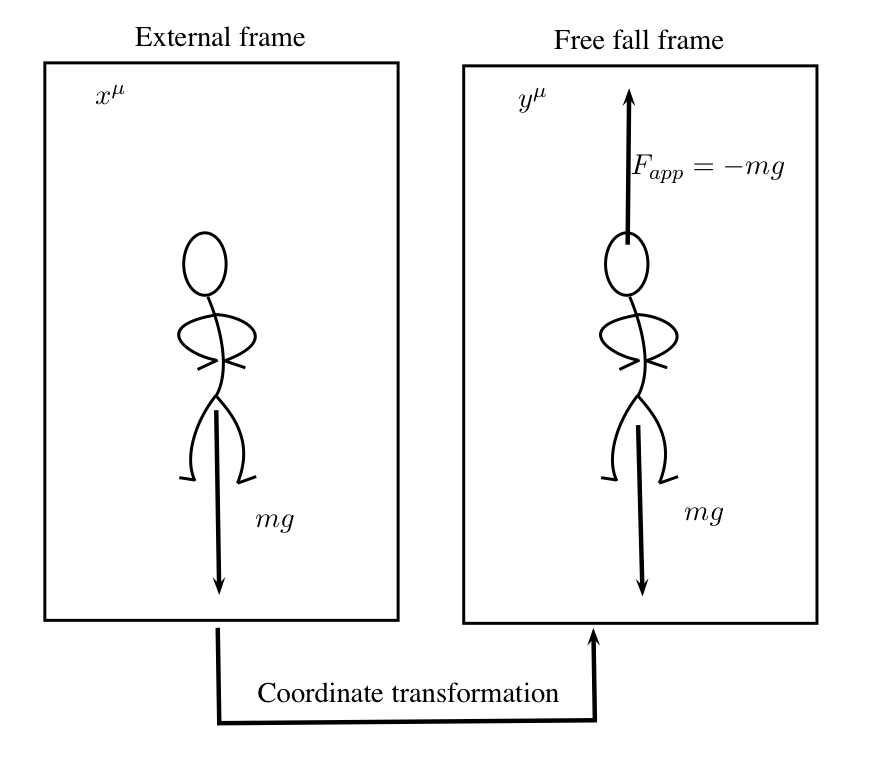
\includegraphics[scale=0.7]{Draw/Free_fall.png}
\label{}
\end{center}
\caption{A guy in a free falling elevator experiencing a zero total force}
\label{freefall}
\end{figure}
A guy is climbing a building in an elevator, at a certain time the elevator breaks and it starts to free fall under earth's gravity. As seen from an external observer, the guy (assuming he's not in contact with the floor) will experience the gravity force $mg$ and hence will accelerate towards the ground. From the accelerating elevator point of view, though, there will be an additional appearent force pointing up and exactly balancing gravity, due to the fact that we are looking at the situation from the point of view of a frame which itself accelerates with acceleration $g$. If we call $x^\mu$ the coordinates (space and time) in the external frame and $y^\mu$ the coordinates in the free falling frame, we see that the coordinate transformation $x\rightarrow y(x)$ brings us from a system in which gravity is present to a system in which gravity is absent. Paraphrasing this in mathematical terms, we can say that, in $y$ coordinates we can express the interval as
\begin{equation}
ds^2=\eta_{\mu\nu}dy^\mu dy^\nu
\end{equation}
We cannot the say the same in $x$ coordinates: we know that the interval $ds^2$ is invariant under coordinate transformations, but since $y$ and $x$ are not connected by a simple lorentz transformation (acceleration is involved), the best we can do is to write $ds^2=\eta_{\mu\nu}dy^\mu dy^\nu=g_{\mu\nu}dx^\mu dx^\nu$ where $g_{\mu\nu}$ is a symmetric $4\times4$ matrix, but it is not in the form \ref{etamunu}. What our coordinate transformation does for us, is that \textit{locally} (in the elevator), it transforms the complicated metric $g_{\mu\nu}$ into the flat one $\eta_{\mu\nu}$. General Relativity is based on this simple idea: this transformation always exists, i.e. it always exists a \textit{local free fall frame} (the analogous of the elevator idea can be applied for example to a spaceship falling in a black hole or on the space shuttle orbiting the earth; why is this a free fall frame?). This is the so called \textit{equivalence principle} which says that, given a generic point in spacetime $x$, in 
which the metric is $g_{\mu\nu}(x)$, it \textit{always} exists a coordinate transformation $y(x)$ such that, \textit{at the point} $y(x)$, the metric is transformed as $g'_{\mu\nu}(y(x))=\eta_{\mu\nu}$. To be a little bit more technical here, by \textit{metric transformation} we intend that, given the fact that the interval is invariant, $ds^2=g_{\mu\nu}(x)dx^\mu dx^\nu=g'_{\mu\nu}(y(x))dy^\mu dy^\nu$, the metric transforms in the way
\begin{equation}
g'_{\mu\nu}=g_{\alpha\beta}\frac{dx^\alpha}{dy^\mu}\frac{dx^\beta}{dy^\nu}
\end{equation}
The important statement here is that, in general, this transformation that locally cancels gravity does the trick $g_{\mu\nu}\rightarrow \eta_{\mu\nu}$ \textit{only at one point}; in general we can't find a coordinate transformation that cancels gravity at every point in space, and this makes sense, because if this would have been possible gravity wouldn't exist at all. For example, thinking back at the guy in the elevator, in his free fall frame he doesn't feel earth's gravity, but if he were to be sensible enough he could still feel the moon's gravitational pull (and the pull from the rest of the solar system as well). Now a tricky question arises: let's consider a generic metric $g_{\mu\nu}$ which describes our spacetime; it might be that $g_{\mu\nu}$ has a special form, such that I can revert it back to $\eta_{\mu\nu}$ all over the place using a particular coordinate transformation. Consider for example the following: 
\begin{equation}
\label{metspher}
ds^2=-c^2dt^2+dr^2+r^2(d\theta^2+\sin^2{\theta}d\phi^2)
\end{equation}
The metric here is not in the form $\eta_{\mu\nu}$, because it depends on the position $x^\mu=(ct,r,\theta,\phi)$; if we go from the spherical coordinates to the cartesian ones through the transformation (see Figure \ref{coordinates}) $(ct,r,\theta,\phi)\rightarrow(ct,x=r\sin{\theta}\cos{\phi},y=r\sin{\theta}\sin{\phi},z=r\cos{\theta})$, we can revert the metric back to the flat form 
\begin{equation}
ds^2=-c^2dt^2+dx^2+dy^2+dz^2
\end{equation}
\begin{figure}
\begin{center}
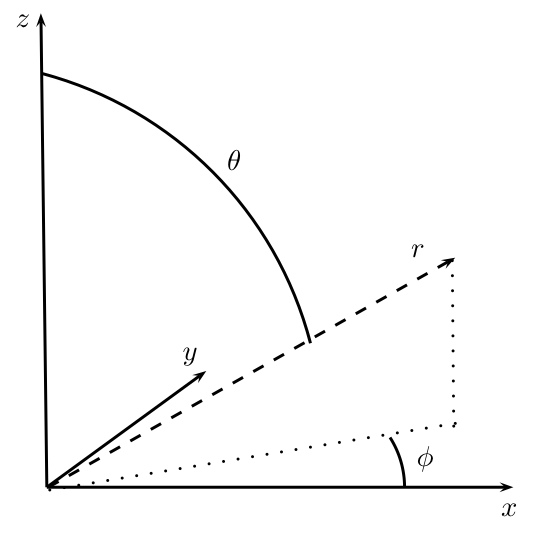
\includegraphics[scale=0.7]{Draw/coordinates.png}
\label{}
\end{center}
\caption{Spherical coordinate system}
\label{coordinates}
\end{figure}
This means that a metric in the form (\ref{metspher}), describes a spacetime which is flat, i.e., in which there are no gravitational forces, even if the metric depends on position. Consider now the following metric
\begin{equation}
\label{blackmetric}
ds^2=-c^2\left(1-\frac{2GM}{rc^2}\right)dt^2+\frac{dr^2}{1-\frac{2GM}{rc^2}}+r^2(d\theta^2+\sin^2{\theta}d\phi^2)
\end{equation}
It can be shown that there exists \textit{no coordinate transformation} that reverts this metric back to $\eta_{\mu\nu}$ in \textit{every} point in space; this is because this metric describes a spacetime in which there is a gravitational source (in particular a star or planet of mass $M$ in this case) and the spacetime is not flat. The question now is: given a generic metric $g_{\mu\nu}(x)$, how can we tell if it describes a flat spacetime or a spacetime is which there is gravity; once again Einstein helps us. The answer is that gravity manifests itself as \textit{curvature} in the spacetime bulk. As we wil understand later, a metric in the form (\ref{blackmetric}) is curved, whereas one in the form (\ref{metspher}) has no curvature and is flat. What do we precisely mean by this? And how do we know if a metric is curved? We will answer this question in the folowing paragraph. 
\subsection{The geometry of spacetime}
In the previous paragraph we have seen that choosing arbitrary coordinate reference frames (which are not necessarily connected by lorentz transformations), changes the metric $g_{\mu\nu}$ in such a way that the interval $ds^2$ is invariant; in this paragraph we want to convince ourselves that the metric $g_{\mu\nu}$ carries all the geometrical information on our spacetime. In particular the metric will do two things for us: 
\begin{itemize}
\item It will tell us how physical bodies should move (i.e. how planets orbit stars, black holes, etc.)
\item It will tell us when and how our spacetime is curved: this will tell us when we are, or we are not, in the presence of a gravitational source
\end{itemize}
Motivated by the study of special relativity, Einstein came up with these two rules for body motions in a spacetime with coordinate $x^{\mu}$ and metric $g_{\mu\nu}$; each physical body will follow a trajectory $x^{\mu}(s)$ such that 
\begin{enumerate}
\item If the body is massles (like a photon, i.e. a light ray) then the trajectory will satisfy $ds^2=g_{\mu\nu}dx^{\mu}dx^{\nu}\equiv 0$; this is the same as saying that massless particles travel at the speed of light
\item If the body has a mass then the trajectory will always satisfy $ds^2<0$ (the body will travel slower than light); moreover, among all the trajectories that connect two points $A$ and $B$, the body will choose that particular trajectory such as 
\begin{equation}
\Delta s_{AB}=\int_A^Bds
\end{equation}
is maximum. All such trajectories are called \textit{geodesics} and are determined entirely by the metric $g_{\mu\nu}$.
\end{enumerate}
The fact that bodies travel along geodesics can be paraphrased saying that bodies, when they move, "follow the geometry of spacetime"; since the metric shapes the trajectories, we can say that the metric encodes the geometry of spacetime. This gives us some insight on how gravity works in this new picture: the sun "curves" the spacetime, modifiying his metric. Planets must follow the geodesic dictated by the metric and hence orbit the sun. But how does the sun curve the spacetime around it? Before answering this question we must first understand what "curvature" actually means. 
\subsection{The meaning of curvature}
Let's think about the following example, involving simple geometrical ideas: a plane is flat, but a sphere is curved. What makes a sphere curved? And more important, can we distinguish a flat plane from a curved sphere just looking at their \textit{intrinsic} properties? (i.e. can we realize that a sphere is curved just sitting on it, without looking at it from the exterior?) It turns out we can, just look at Figure \ref{sphere}
\begin{figure}
\begin{center}
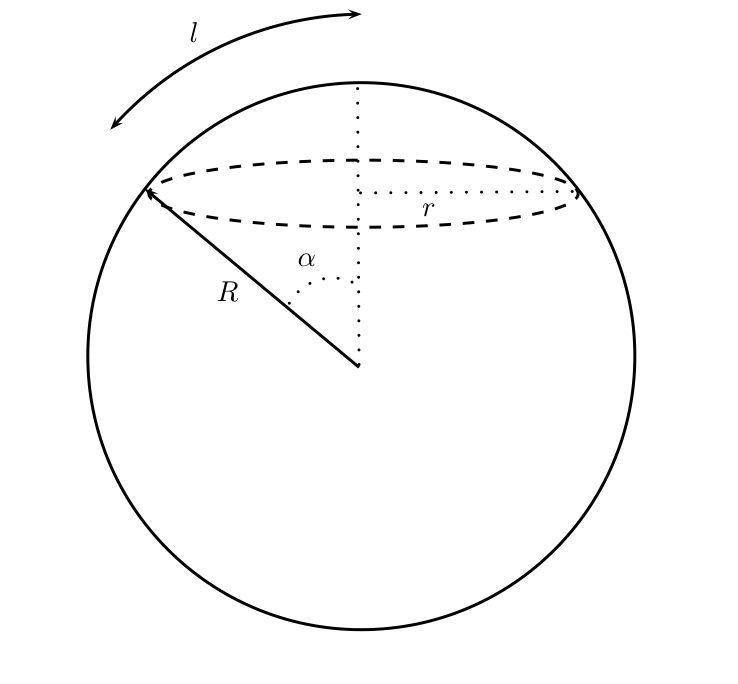
\includegraphics[scale=0.7]{Draw/sphere.png}
\end{center}
\caption{Example on why a sphere is curved}
\label{sphere}
\end{figure}
Suppose we have a rope of length $l$ which we fix, at one extreme, at the north pole; sitting on the sphere, we can measure two things: the length of the dashed circle (which is the collection of all the points touched by the rope as we go around one full turn) and the area on the sphere enclosed by it. Suppose that we know the value of $\pi$; let's call $C$ and $A$ the length of the circle and the area that we physically measure sitting on the sphere. If we were on a plane we would expect $C=2\pi l$ and $A=\pi l^2$, but looking again at Figure \ref{sphere}, you can convince yourselves that this is not the case. In fact we have (take the second relation for granted)
\begin{equation}
C=2\pi R\sin{\alpha}=2\pi R\sin{\left(\frac{l}{R}\right)}
\end{equation}
\begin{equation}
A=R^2\int_0^{2\pi}d\phi\int_0^{\alpha}\sin{\theta}d\theta=2\pi R^2(1-\cos{\alpha})=2\pi R^2\left[1-\cos{\left(\frac{l}{R}\right)}\right]
\end{equation}
And the relative corrections from the results we obtain on flat space are
\begin{equation}
\frac{C}{2\pi l}=\frac{R}{l}\sin{\left(\frac{l}{R}\right)}
\end{equation} 
\begin{equation}
\frac{A}{\pi l^2}=2\left(\frac{R}{l}\right)^2\left[1-\cos{\left(\frac{l}{R}\right)}\right]
\end{equation}
Now imagine that the radius $R$ of the sphere is very big, so big that if our rope is not so big, we barely notice the change: for $\alpha=l/R\ll 1$ we Taylor approximate $\sin{\alpha}\approx \alpha - \alpha^3/6$ and $\cos{\alpha}\approx1-\alpha^2/2+\alpha^4/24$ and we get 
\begin{equation}
\frac{C}{2\pi l}\approx 1-\frac{1}{6}\left(\frac{l}{R}\right)^2
\end{equation}
\begin{equation}
\frac{A}{\pi l^2}\approx 1-\frac{1}{12}\left(\frac{l}{R}\right)^2
\end{equation}
These relations tell us a couple of interesting facts:
\begin{itemize}
\item If the radius of the sphere is really big, and we don't go to far from the center with our rope, we barely notice the difference from being on a regular flat plane
\item The measurements of length and area that we get on the sphere are \textit{smaller} than those that we get on the plane (look at the minus sign): we conventionally refer this type of curvature as \textit{positive} curvature
\item Whatever curvature is, it's characterized by a length scale, in this case the radius of the sphere $R$, and all the corrections from flat space are proportional to $l^2$ that is to say to the area enclosed by our experiment
\end{itemize}
Believe it or not, these three facts will be enough to get a basic understanding on where the curvature comes in when we consider a spacetime metric $g_{\mu\nu}$ 
\begin{figure}
\begin{center}
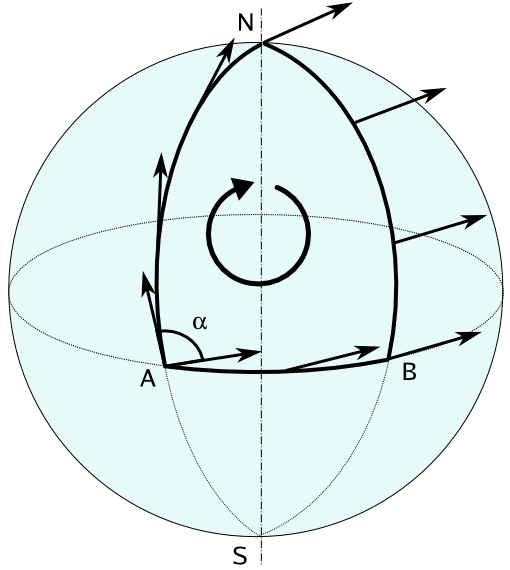
\includegraphics[scale=0.5]{Draw/Parallel_transport.png}
\end{center}
\caption{Parallel transport of a vector around a closed loop $A\rightarrow B\rightarrow N \rightarrow A$: on a curved space the vector will be tilted when it comes back to $A$, and the tilt will be proportional to the area enclosed by the loop. Source \url{http://en.wikipedia.org/wiki/File:Parallel_transport.png}}
\label{transport}
\end{figure}
Consider a situation similar to Figure \ref{transport}; you can generalize this conclusions to an arbitrary curved space: consider a vector $v^\mu$, and a closed loop $ABNA$ on the surface. Imagine to \textit{transport} this vector around the loop in such a way that, on each part of the loop, the vector forms a constant angle with the \textit{tangent} to the loop; this way of moving vectors is called \textit{parallel transport}. When the vector comes back to the original point, if the surface is curved, it will be tilted, and this tilt will be proportional to the area enclosed by the loop. Now consider a very small loop of sides $dx^\mu$ and $dx^\nu$ like in Figure \ref{loop}
\begin{figure}
\begin{center}
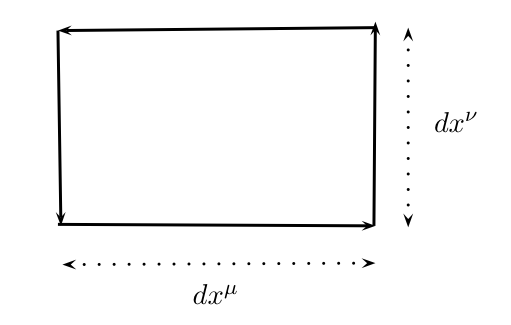
\includegraphics[scale=0.8]{Draw/loop.png}
\end{center}
\caption{A small loop on a curved surface}
\label{loop}
\end{figure}
If we parallel transport a vector along this loop it will undergo a change $\Delta v^\lambda$ proportional to the area $dx^\mu dx^\nu$; the change will also be proportional to the vector itself, since if we transport a vector with all zero components, it make sense that the transported vector will remain zero. Hence the change must be proportional to $\Delta v^\lambda\propto v^\rho dx^\mu dx^\nu$; the thing that we miss is the curvature, i.e. the 1/(length scale)$^2$; since we want this to be an invariant statement, we see that the curvature cannot be a simple number, but must be at least a tensor with 4 indices, and this must have measure units (length)$^{-2}$, this will be the first rigorous definition of curvature we encounter
\begin{equation}
\Delta^{loop}v^\lambda=R_{\mu\nu\rho}^\lambda v^\rho dx^\mu dx^\nu
\end{equation}
This $R_{\mu\nu\rho}^\lambda$ is called \textit{riemann tensor} and we claim that it can be calculated \textit{directly} from the metric: it measures the curvature, in the sense that if it is 0 then the space is flat and there are no gravitational sources, but if it is non zero then it means that the space is curved and there must be some curving source in it. The fact that the riemann tensor can be calculated directly from the metric is due to the fact that, given a geodesic, it can be shown that its tangent vector is parallel transported along it. Since geodesics are defined by the metric and are connected to parallel transport, then the curvature must be expressed as some (even if complicated) function of the metric. Once we understand this, then the jump to the final new picture of gravity is simple (but it took Einstein to make it!): the sun (and matter in general) curves the space around the planets. The planets' orbits are the geodesics in this curved metric. The statement "matter curves space" is 
expressed mathematically as Einstein equation, which has the general form
\begin{equation}
\label{einsteinsymb}
\mathrm{(Some \,\,function\,\, of }\,R_{\mu\nu\lambda}^\rho[g_{\mu\nu}] \mathrm{ \,\,and\,\, } g_{\mu\nu})= \mathrm{(Some\,\, tensor \,\,that\,\, describes\,\, matter)}
\end{equation}
Describing the motion of planets now becomes the following process: find the sun's distortion to the flat metric solving Einstein's equation (\ref{einsteinsymb}) and then find the geodesics in this metric. In the solar system this method gives results which are very close to the newtonian ones, except that contrary to Newton, the Einstein's equation predicts the correct Mercury's perihelion precession.


\chapter{General Relativity and the fundamental observations of cosmology}

\section{General Relativity}

We have seen in the previous lecture how the incompatibility between Newtonian gravity and Special Relativity, in addition to the equivalence principle, leads us to the new picture of General Relativity (GR), in which the effects of gravity are described by the curvature of spacetime. As we learned in lecture 2, all the geometrical properties of a space (or a spacetime in the case of GR) are encoded in the metric tensor, so it is natural to regard the metric as the gravitational field that affects the motion of particles. It remains to understand how do we calculate the metric in the first place. This will be the subject of this section.

\subsection{The motion of particles and geodesics}

Let us begin by summarizing what we learned in the previous lecture about the relation between the motion of particles and the metric of spacetime. Given two events with spacetime coordinates $(x^0,x^1,x^2,x^3)$ and $(x^0+dx^0,x^1+dx^1,x^2+dx^2,x^3+dx^3)$,\footnote{In chapter 2 we defined $x^0=ct$, $x^1=x$, $x^2=y$, $x^3=z$. Here we will abandon this convention; the coordinates $x^{\mu}$ now refer to an arbitrary coordinate system. For example, in spherical coordinates (see chapter 3) we would have $x^0=ct$, $x^1=r$, $x^2=\theta$, $x^3=\phi$. (We will always consider coordinate systems in which $x^0$ is a time coordinate and $x^1$, $x^2$, $x^3$ are spatial coordinates; however, there are examples of coordinate systems in which this not the case.)} the spacetime interval $ds$ between them is given by
\begin{equation} \label{eq:line_element}
ds^2=g_{\mu\nu}dx^{\mu}dx^{\nu}.
\end{equation}
Remember that in GR the metric is a function of spacetime, i.e.\ $g_{\mu\nu}=g_{\mu\nu}(x^0,x^1,x^2,x^3)$. It is only in SR (that is, in the absence of gravity) that we can find coordinates where $g_{\mu\nu}$ is constant everywhere. We can consider these two events to be related to a particle located at position $(x^1,x^2,x^3)$ at time $x^0$, and then located at $(x^1+dx^1,x^2+dx^2,x^3+dx^3)$ at time $x^0+dx^0$. This is simply a way of keeping track of the particle's motion by means of successive, infinitesimally close events.

Recall that for a particle we have $ds^2<0$. This is easy to see in SR, where we can choose a Cartesian coordinate system $(ct,x,y,z)$ in which $g_{\mu\nu}=\eta_{\mu\nu}$. If we assume that the particle is moving in the $x$-direction, so that $dy=0$ and $dz=0$, then eq.\ (\ref{eq:line_element}) becomes
\begin{equation}
\begin{split}
ds^2&=-c^2dt^2+dx^2\\
&=-dt^2\left(c^2-\left(\frac{dx}{dt}\right)^2\right)\\
&=-dt^2\left(c^2-v^2\right),
\end{split}
\end{equation}
where $v=dx/dt$ is the velocity of the particle. Since the particle cannot move faster than light, we must have that $(c^2-v^2)>0$, and therefore $ds^2<0$. Having shown that $ds^2<0$ in SR, we can immediately conclude that $ds^2<0$ also in GR. This follows from the fact that at any point in a curved spacetime we can choose coordinates where, in a small neighborhood around the point, the metric is $g_{\mu\nu}\approx\eta_{\mu\nu}$.

The {\it proper time} $d\tau$ elapsed along a particle's trajectory is defined as
\begin{equation} \label{eq:proper_time_dtau}
d\tau=\sqrt{-\frac{ds^2}{c^2}}=\frac{1}{c}\sqrt{-g_{\mu\nu}dx^{\mu}dx^{\nu}}.
\end{equation}
Notice that the expression inside the square root is positive since $ds^2<0$ for a particle, and therefore $d\tau$ is a positive real quantity. The above definition holds for an infinitesimal path, but we can find the proper time elapsed along a finite trajectory by integrating $d\tau$ along the path traveled by the particle. Thus, if a particle moves from some spacetime point $A$ to some other spacetime point $B$, then the proper time along the path is given by
\begin{equation}
\begin{split}
\Delta\tau(A\to B)&=\int_A^B d\tau\\
&=\frac{1}{c}\int_A^B \sqrt{-g_{\mu\nu}dx^{\mu}dx^{\nu}}.\\
\end{split}
\end{equation}
Physically, the proper time corresponds to the time measured by a clock moving together with the particle. Notice that, although the spacetime interval along a particle's path cannot be measured using rulers, it can be measured using a clock.

Given the trajectory that a particle travels we now know how to compute the proper time elapsed from the initial point $A$ to the final point $B$ of the path. But suppose we are given nothing but the spacetime coordinates of the points $A$ and $B$, and we are asked to find the path that a particle takes when going from $A$ to $B$. Among all the possible paths the particle can take between $A$ and $B$, the actual path will be the one that {\it maximizes} the elapsed proper time $\Delta\tau(A\to B)$. With this prescription, we can in principle predict the motion of particles from the knowledge of the metric of the spacetime.

From a geometrical point of view, the trajectories that maximize the proper time between two given points are called {\it geodesics} of the spacetime. Geodesics are easy to visualize in 2-dimensional spaces; in this case we do not have to deal with proper time (there is no time dimension) and $ds$ is the usual length we would measure with a ruler. Thus, given two points $A$ and $B$, the length of a path connecting them is simply
\begin{equation}
\Delta s(A\to B)=\int_A^B ds.
\end{equation}
The geodesic is then given by the path that {\it minimizes} $\Delta s(A\to B)$.\footnote{Notice that in spacetimes geodesics are the paths that maximize the proper time, whereas in spaces (no time dimension) geodesics are the paths that minimize the length. The reason for this difference has to do with the fact that $ds^2$ is not necessarily positive in spacetimes.} Fig.\ \ref{fig:lec4_1} shows two examples of 2-dimensional spaces, the flat plane and the sphere. Clearly, the geodesics on the plane correspond to straight lines; any other curve joining two given points will obviously have a larger length. Perhaps less obvious is that the geodesics on the sphere correspond to circular segments around the center of the sphere. For example, if point $A$ is the north pole of the sphere and $B$ is a point on the equator, then the geodesic connecting $A$ and $B$ goes along ``meridian'' through these points.
\begin{figure}[ht]
\begin{center}
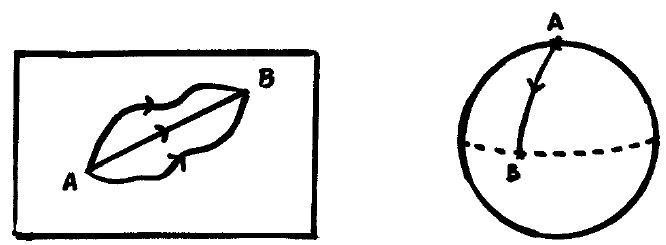
\includegraphics[scale=0.5]{Draw/lec4_1.png}
\end{center}
\caption{Geodesics in 2-dimensional spaces}
\label{fig:lec4_1}
\end{figure}

One final quantity that we need to define, which we will need later, is the {\it 4-velocity} of a particle. Since the proper time $\tau$ is a quantity that increases monotonically along a particle's trajectory, we can use it to parametrize the path traveled by the particle. In other words, we can think of the spacetime coordinates $x^{\mu}$ of the particle as being functions of $\tau$, i.e.\ $x^{\mu}(\tau)$. The 4-velocity of the particle is then defined as
\begin{equation}
U^{\mu}\equiv \frac{dx^{\mu}}{d\tau}.
\end{equation}
Of course, the coordinates $x^{\mu}$ refer to a specific coordinate system, and therefore $U^{\mu}$ will depend on the specific coordinate system or reference frame we are using. As an example, consider a reference frame where a particle is at rest. Since the particle is not moving in space, we have that $x^1$, $x^2$ and $x^3$ are constants, and therefore $U^i=dx^i/d\tau=0$.\footnote{Recall that greek indices range from 0 to 3, whereas latin indices range from 1 to 3.} On the other hand, the time coordinate $x^0$ is equal to $c\tau$, since by definition $\tau$ is the time measured in the frame where the particle is at rest. Therefore $U^0=dx^0/d\tau=d(c\tau)/d\tau=c$. In summary, the 4-velocity vector of a particle at rest is given by $(c,0,0,0)$.

A useful property of the 4-velocity that we will use later is that it is {\it normalized}. What this means is simply that $g_{\mu\nu}U^{\mu}U^{\nu}$ has a constant value which turns out to be $-c^2$. Indeed, using the definition of $U^{\mu}$ and eq.\ (\ref{eq:proper_time_dtau}), we have
\begin{equation}
\begin{split}
g_{\mu\nu}U^{\mu}U^{\nu}&=g_{\mu\nu}\frac{dx^{\mu}}{d\tau}\frac{dx^{\nu}}{d\tau}\\
&=\frac{g_{\mu\nu}dx^{\mu}dx^{\nu}}{d\tau^2}\\
&=\frac{ds^2}{-ds^2/c^2}=-c^2
\end{split}
\end{equation}
\begin{equation}
\Rightarrow~~~~g_{\mu\nu}U^{\mu}U^{\nu}=-c^2.
\end{equation}


\subsection{The Einstein equations}

We know how to calculate the motion of particles in spacetime if we know the metric. But how do we find the metric in the first place? In principle we could measure the metric by observing how particles move, but unless we do such observations on all points in space at all times (which is obviously impractical), we will never know what the metric is everywhere in the spacetime. Instead, we would like to be able to calculate the metric starting from the knowledge of the sources of the gravitational field. For example, in Newtonian physics, just by knowing the mass of the Sun we can find the (approximate) gravitational field in the whole solar system, thanks to Newton's law of gravitation.

The analog of Newton's law in GR is given by the {\it Einstein equations}:
\begin{equation} \label{eq:einstein_eqs}
G^{\mu\nu}=\frac{8\pi G}{c^4}T^{\mu\nu},
\end{equation}
where $G$ is Newton's constant (the same that appears in Newton's law), $c$ is the speed of light, $G^{\mu\nu}$ is the {\it Einstein tensor}, and $T^{\mu\nu}$ is the {\it energy-momentum tensor}. The Einstein tensor is quite complicated and so we will not give its precise definition. The only thing you need to know about it is that it depends solely on the metric (and on first and second derivatives of the metric) through the Riemann tensor (see chapter 3), which means that $G^{\mu\nu}=0$ when the spacetime is flat, since the Riemann tensor vanishes everywhere in Minkowski spacetime.

The energy-momentum tensor (also known as the stress-energy tensor), as it name suggests, depends on the energy and momentum of the sources present in the spacetime (and also possibly on the metric). There is no general explicit formula for $T^{\mu\nu}$, since it will depend on what kind of sources we are dealing with; in the next section we will see an example relevant to cosmology. We remarked in chapter 2 that in relativity energy and momentum should not be considered as independent entities, since energy can be transformed into momentum, and vice versa, by means of a Lorentz transformation. It should not be surprising then that it is both the energy {\it and} the momentum of the sources what gives rise to a gravitational field. This is in marked contrast to what happens in Newtonian gravity, where only the mass (which, as you know, is a form of energy) is relevant in the gravitational interaction.

Both $G^{\mu\nu}$ and $T^{\mu\nu}$ are symmetric tensors, which means that
\begin{equation}
G^{\mu\nu}=G^{\nu\mu},\mbox{ and }~~T^{\mu\nu}=T^{\nu\mu}.
\end{equation}
This implies that, although there are 16 possible combinations for the indices $\mu\nu$, the Einstein equations are really 10 independent equations. This correctly matches the number of independent components of the metric $g_{\mu\nu}$, which you may remember is also a symmetric tensor.

\par\vspace{\baselineskip}

{\bf Exercise.} Show that a symmetric $4\times4$ matrix has 10 independent components.

\par\vspace{\baselineskip}

\section{Perfect fluids}

A fluid is a continuous substance that can be deformed under the application of a force or stress. A fluid has no fixed shape, and will tend to assume the shape of its container. Fig.\ \ref{fig:lec4_2} shows a volume of fluid in which several {\it fluid elements} have been drawn. A fluid element is a portion of the fluid that is macroscopically small, meaning that we can approximate it as being homogeneous, but microscopically large, meaning that it contains a very large number of particles so that a fluid description is appropriate. The fact that a fluid element is homogeneous implies that it can be characterized by its density $\rho$ (mass per unit volume), its pressure $p$ (force per unit area exerted perpendicularly on its neighbors), its shear viscosity $f_s$ (the antislipping force; see fig.\ \ref{fig:lec4_2}), and its 4-velocity $U^{\mu}$. A {\it perfect fluid} is one where $f_s=0$ for all fluid elements. It turns out that many sources of energy in astrophysics and cosmology can be well approximated 
as perfect fluids, and so we will focus on them in the following discussion.
\begin{figure}[ht]
\begin{center}
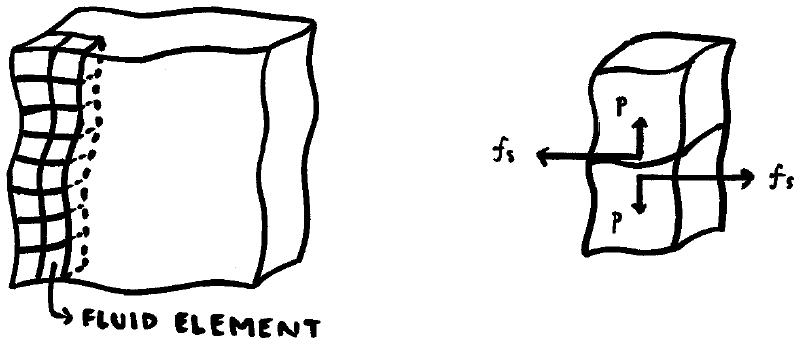
\includegraphics[scale=0.5]{Draw/lec4_2.png}
\end{center}
\caption{Perfect fluids}
\label{fig:lec4_2}
\end{figure}

After defining the properties of individual fluid elements, we can extend these definitions to the whole fluid. We will characterize a fluid by the three functions $\rho(t,x,y,z)$, $p(t,x,y,z)$, and $U^{\mu}(t,x,y,z)$, which are defined as:\footnote{Here we are using the familiar Cartesian coordinates $(t,x,y,z)$ just to make the discussion simpler, but note that all these definitions can be applied in an arbitrary reference frame with coordinates $(x^0,x^1,x^2,x^3)$.}
\begin{itemize}
\item $\rho(t,x,y,z)$ is the density of the fluid element located at the position $(x,y,z)$ at the time $t$.
\item $p(t,x,y,z)$ is the pressure of the fluid element located at the position $(x,y,z)$ at the time $t$.
\item $U^{\mu}(t,x,y,z)$ is the 4-velocity of the fluid element located at the position $(x,y,z)$ at the time $t$.
\end{itemize}
With these definitions we can now write down the energy-momentum tensor of a perfect fluid:
\begin{equation} \label{eq:perfect_fluid_tmunu}
T^{\mu\nu}=\left(\rho+\frac{p}{c}\right)U^{\mu}U^{\nu}+pcg^{\mu\nu}.
\end{equation}
Here the tensor $g^{\mu\nu}$ corresponds, by definition, to the components of the {\it matrix inverse} of $g$. Recall that, given a matrix $M$, its inverse matrix is defined as the matrix $M^{-1}$ such that $MM^{-1}=I$ (where $I$ is the identity matrix). As an example, consider the Minkowski metric,
\begin{equation}
\eta=\left( \begin{array}{cccc} -1 & 0 & 0 & 0 \\ 
0 & 1 & 0 & 0 \\
0 & 0 & 1 & 0 \\
0 & 0 & 0 & 1\end{array} \right).
\end{equation}
Its inverse matrix is given by
\begin{equation}
\eta^{-1}=\left( \begin{array}{cccc} -1 & 0 & 0 & 0 \\ 
0 & 1 & 0 & 0 \\
0 & 0 & 1 & 0 \\
0 & 0 & 0 & 1\end{array} \right).
\end{equation}
We leave as an excercise for you to check that
\begin{equation}
\eta\eta^{-1}=\left( \begin{array}{cccc} 1 & 0 & 0 & 0 \\ 
0 & 1 & 0 & 0 \\
0 & 0 & 1 & 0 \\
0 & 0 & 0 & 1\end{array} \right)=I.
\end{equation}
In this example we have that $\eta^{-1}=\eta$. However, note that this will not be true for a general metric $g$. That is why we need to distinguish $g_{\mu\nu}$ (the components of the metric $g$) from $g^{\mu\nu}$ (the components of the inverse metric $g^{-1}$).

\par\vspace{\baselineskip}

{\bf Exercise.} Consider the metric given by
\begin{equation}
ds^2=-c^2dt^2+Adx^2+Bdy^2+Cdz^2,
\end{equation}
where $A$, $B$, and $C$ are positive constants, and the coordinate system is $(ct,x,y,z)$.
\begin{itemize}
\item [(a)] Show that the components $g_{\mu\nu}$ of the metric are given by
\begin{equation}
g_{00}=-1,~~~~g_{11}=A,~~~~g_{22}=B,~~~~g_{33}=C,
\end{equation}
with all other components equal to zero.
\item [(b)] Write the metric in matrix form as
\begin{equation}
g=\left( \begin{array}{cccc} -1 & 0 & 0 & 0 \\ 
0 & A & 0 & 0 \\
0 & 0 & B & 0 \\
0 & 0 & 0 & C\end{array} \right),
\end{equation}
and from this find the inverse metric $g^{-1}$. Show that the components $g^{\mu\nu}$ of $g^{-1}$ are given by
\begin{equation}
g^{00}=-1,~~~~g^{11}=\frac{1}{A},~~~~g^{22}=\frac{1}{B},~~~~g^{33}=\frac{1}{C},
\end{equation}
with all other components equal to zero. Note that $g^{-1}\neq g$ in this example.
\end{itemize}

\par\vspace{\baselineskip}

Given a perfect fluid with some specified density $\rho(t,x,y,z)$, pressure $p(t,x,y,z)$, and 4-velocity $U^{\mu}(t,x,y,z)$, we could compute the energy-momentum tensor $T^{\mu\nu}$ from eq.\ (\ref{eq:perfect_fluid_tmunu}), plug the result in the Einstein equations (\ref{eq:einstein_eqs}), and solve for the metric $g_{\mu\nu}$ (in practice this can be very difficult though). As an example, let us find $T^{\mu\nu}$ for a perfect fluid at rest in Minkowski spacetime (i.e.\ $g_{\mu\nu}=\eta_{\mu\nu}$). Since the fluid is at rest, we have that the components of the 4-velocity are $U^0=c$ and $U^i=0$. Then we find
\begin{equation}
\begin{split}
T^{00}&=\left(\rho+\frac{p}{c}\right)U^{0}U^{0}+pc\eta^{00}\\
&=\left(\rho+\frac{p}{c}\right)c^2-pc=\rho c^2,
\end{split}
\end{equation}
and
\begin{equation}
T^{11}=pc\eta^{11}=pc,~~~~T^{22}=pc\eta^{22}=pc,~~~~T^{33}=pc\eta^{33}=pc.
\end{equation}
You can easily check that all other components of $T^{\mu\nu}$ vanish. Therefore we can write, in matrix form,
\begin{equation}
T^{\mu\nu}=\left( \begin{array}{cccc} \rho c^2 & 0 & 0 & 0 \\ 
0 & pc & 0 & 0 \\
0 & 0 & pc & 0 \\
0 & 0 & 0 & pc\end{array} \right).
\end{equation}


\section{Cosmology: Fundamental observations}

We are now ready to begin our study of cosmology. In this section we will cover the fundamental observational facts about the universe. We will see how these facts can be explained by the Big Bang model, in which the universe was born from an initial singularity and has been expanding ever since. These observations will also guide us in the task of modeling the universe mathematically in the framework of GR.

\subsection{The Olbers paradox}

Why is the night sky dark? This simple question summarizes what is known as the Olbers paradox. The paradox arises when we think of the universe as being static, infinitely old, infinitely large, and with an infinite number of stars. If we lived in such a universe, then in every direction we looked at in the night sky we should encounter a star along the line of sight, simply because there are infinitely many stars. The night sky should therefore be completely bright!

Let us look at this argument more closely. One could argue that our conclusion is incorrect because distant stars appear dimmer, and so they may not be visible in the night sky. Thus, if in one direction in the sky there were no nearby stars, then the night sky would be dark in that direction. This objection is wrong, however, because although the apparent brightness of stars decreases with distance, the number of stars along a given line of sight increases. This is illustrated in fig.\ \ref{fig:lec4_3}. Here $A$ and $B$ denote two directions in the sky; in direction $A$ we can see some nearby stars, which appear bright, whereas in direction $B$ we do not see nearby stars, but only dimmer stars that are farther away. Does the sky appear brighter in direction $A$ than in direction $B$? No, because in direction $B$ we also see more stars than in direction $A$. This is because our telescope collects light from a larger area in the sky as it observes at larger distances. This area is proportional to the square 
of the distance (since the area of a sphere is proportional to the radius squared), whereas the apparent brightness is inversely proportional to the distance squared.\footnote{To understant why the apparent brightness of a light source is proportional to the inverse squared distance, note that the energy per unit time (or luminosity) crossing a spherical surface of radius $R$ centered on the source is independent of $R$, since all the energy emitted by the source in some time interval must eventually reach the surface (assuming nothing absorbs the energy along the way). However, the energy flux (energy per unit time per unit area) is obtained by dividing the luminosity by the area of the surface, which is proportional to $R^2$.} Therefore the sky in direction $B$ appears as bright (on average) as in direction $A$.
\begin{figure}[ht]
\begin{center}
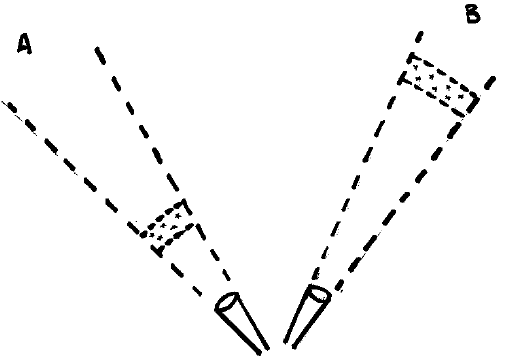
\includegraphics[scale=0.5]{Draw/lec4_3.png}
\end{center}
\caption{The Olbers paradox}
\label{fig:lec4_3}
\end{figure}

The paradox forces us to conclude that this model of the universe (static, infinitely old, infinitely large) must be incorrect. The universe is neither static nor infinitely old, but has some finite age and it is actually expanding, as predicted by the Big Bang model. The fact that the universe has a finite age immediately solves the Olbers paradox: even though the universe might be infinite in space and filled with an infinite number of stars, the light from very distant stars has not had enough time to reach us yet.

\subsection{The cosmological principle: the universe is homogeneous and isotropic}

On very large distance scales, larger than of order $100$ Mpc,\footnote{Recall that $1~{\rm pc}=3.3~{\rm ly}=3.1\times10^{16}$ m. Also, $1~{\rm Mpc}=10^6$ pc.} the universe is observed to be homogeneous and isotropic. This is the cosmological principle, which is essentially the statement that there are no special points in the universe. To be precise, homogeneous and isotropic spaces are defined as follows:
\begin{itemize}
\item {\bf Homogeneous space:} A space with no preferred locations; all points are equivalent.
\item {\bf Isotropic space:} A space where, around one or more points, there are no preferred directions; things look the same in every direction.
\end{itemize}
Notice that isotropy refers to a specific point in a space. For example, a cone is isotropic about the point at its vertex, but not about any other point (fig.\ \ref{fig:lec2_4}). The cone is actually an example of a space that is isotropic but not homogeneous, since clearly the vertex is a special point.\footnote{Notice that the space we are referring to is the 2-dimensional surface of the cone. We can of course visualize the cone as embedded in our 3-dimensional Euclidean space, but the properties of homogeneity and isotropy refer to the 2-dimensional surface in this example (as well as in the examples of the plane and the cylinder discussed next), and are completely independent on how the surface looks as viewed from outside.} The 2-dimensional surface of an infinite cylinder provides an example of a space that is homogeneous (since all points are equivalent) but not isotropic (since a person living in this 2-dimensional space would conclude that not all directions are equivalent; if he walked in the 
direction perpendicular to the axis of the cylinder he would return to the place where he started after some time, whereas this would not be true if he walked in the direction parallel to the axis).
\begin{figure}[ht]
\begin{center}
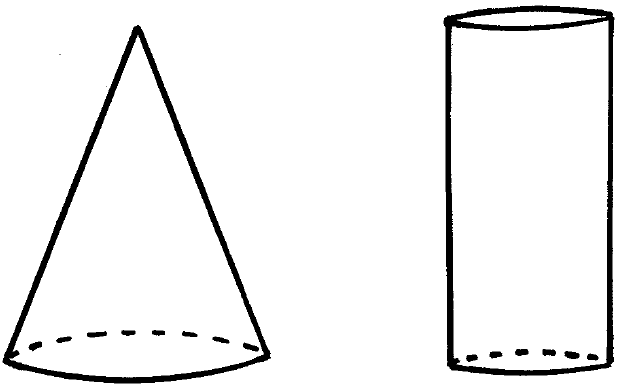
\includegraphics[scale=0.4]{Draw/lec4_4.png}
\end{center}
\caption{Homogeneous and isotropic spaces}
\label{fig:lec4_4}
\end{figure}

From the above examples we see that homogeneity and isotropy are really different concepts. However, if a space is isotropic around not just a few points but around {\it every} point, then it must also be homogeneous (if everything looks the same everywhere, then everywhere is the same). Spaces that are both homogeneous and isotropic are called {\it maximally symmetric spaces}. Examples of maximally symmetric spaces in 2 dimensions are the infinite flat plane and the surface of a sphere. Can you think of other examples? There is in fact one more maximally symmetric space, called the 2-dimensional hyperbolic space, which cannot be visualized (it cannot be embedded in our 3-dimensional Euclidean space, unlike the sphere). It turns out that this is true for any number of spatial dimensions. In 3 dimensions, for instance, the flat space (Euclidean space), the 3-sphere (the 3-dimensional analog of the the usual sphere), and the 3-dimensional hyperbolic space are the only examples of maximally symmetric spaces.\
footnote{The fact that there are exactly three examples of maximally symmetric spaces for any number of dimensions is actually true even if one of the dimensions is a time dimension. This will not be important for us, however. When we say that the universe is homogeneous and isotropic we are talking about the 3-dimensional space, without including the time dimension.} This fact will be important when we go to the task of writing down the possible metrics that can in principle describe our universe.

Returning to the cosmological principle, it is important to emphasize that the principle holds only for large scales. The universe is obviously neither homogeneous nor isotropic on small scales. For example, in the solar system clearly the position of the Sun is a special point, so there is no homogeneity. Also, the solar system has no isotropy, not even around the Sun, since clearly the direction parallel to the plane where the planets move is different from the direction perpendicular to it. It is only when we get to distance scales of order 100 Mpc that the universe begins to look homogeneous and isotropic. Fig.\ \ref{fig:lec4_5} shows an image of the universe as seen from the Earth containing over 2 million galaxies. Make an imaginary square with sides measuring about a tenth of the length of the image; the size of this square is a few hundred megaparsecs. You can see that as you move the square around the image, the number of galaxies contained inside is roughly the same no matter where you locate the 
square. This means that, on the scale of your square, the universe is homogeneous. Also, the galaxies contained inside the square, at any location, clearly do not distribute themselves with some preferred direction, meaning that on this scale the universe is also isotropic.
\begin{figure}[ht]
\begin{center}
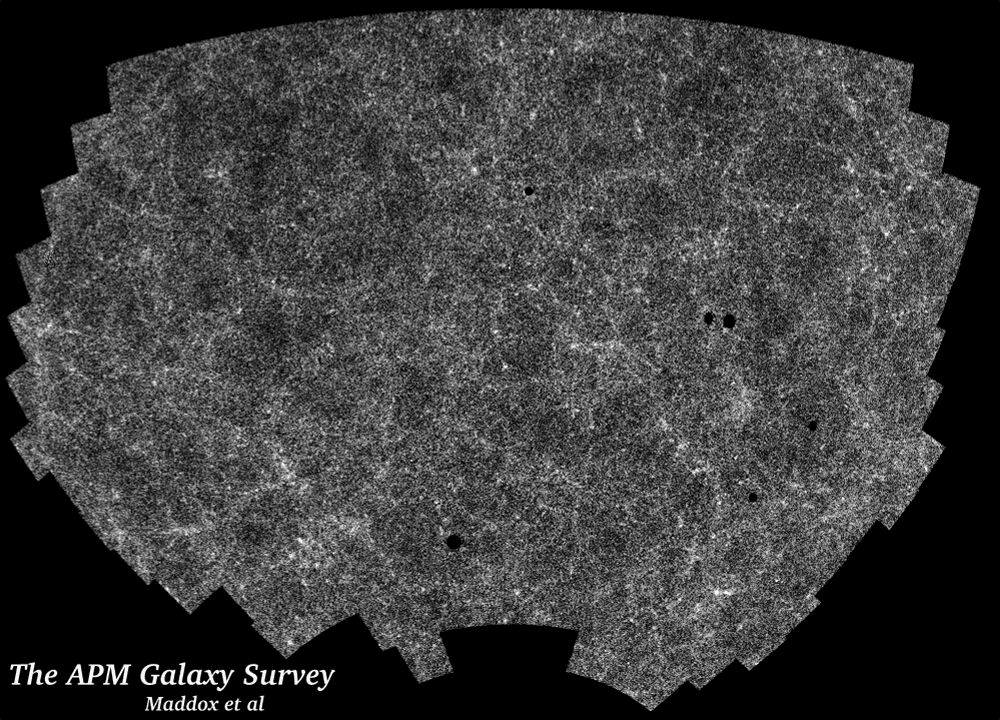
\includegraphics[scale=0.4]{Draw/lec4_5.png}
\end{center}
\caption{The APM Galaxy Survey (Image credit: Maddox et al., The University of Nottingham)}
\label{fig:lec4_5}
\end{figure}

\subsection{The universe is expanding}

In 1929 Edwin Hubble made one of the most extraordinary discoveries in the history of physics: the universe is expanding. This observational fact was the main motivation for the introduction of the Big Bang model, which provides the currently accepted theory of the evolution of the universe. It is fair to say, then, that Hubble's discovery marks the birth of modern cosmology.

Before going into a precise description of Hubble's observation, what is known as Hubble's law, we first need to introduce the concept of redshift in waves and explain the relativistic Doppler effect.

\subsubsection{Waves}

A wave is an oscillatory disturbance that transfers energy and momentum from one point to another, often without transferring particles or mass. Familiar examples include water waves, sound waves, and the waves on a string. These are all examples of {\it mechanical waves}, which are defined as waves that propagate through a medium whose material is deformed by the wave. Other types of waves include electromagnetic waves, gravitational waves, and quantum mechanical matter waves.

Waves can be characterized by their wavelength, frequency, and propagation speed. The wavelength $\lambda$ is given by the distance between two successive crests. Then, if $v$ is the speed of propagation (which depends on both the type of wave and the medium\footnote{The speed of propagation can also depend on the wavelength, in which case the wave is said to be dispersive. Water waves give an example of dispersive waves. We will be mainly interested in electromagnetic waves traveling in vacuum, which are not dispersive; in this case the speed of propagation is always $c$, regardless of the value of $\lambda$.}), the frequency is given by
\begin{equation}
f=\frac{v}{\lambda}.
\end{equation}
The frequency is a measure of the number of oscillations per unit time in a given point on the wave, and it is directly related to the energy transferred by the wave. Thus higher frequency means higher energy, and also longer wavelength. Fig.\ ?? shows the electromagnetic spectrum, the spectrum containing all different types of electromagnetic waves, from the most energetic ones (gamma rays) to the less energetic ones (radio waves). You can see that visible light, the only electromagnetic wave that the human eye can directly observe, constitutes only a small part of the complete spectrum.
\begin{figure}[ht]
\begin{center}
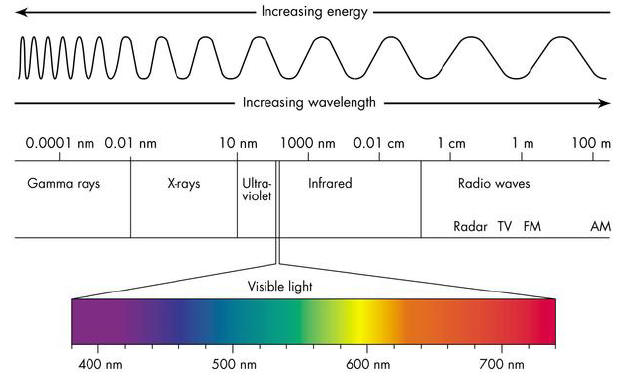
\includegraphics[scale=2]{Draw/lec4_6.png}
\end{center}
\caption{The electromagnetic spectrum (Source: \url{http://www.scimad.com})}
\label{fig:lec4_6}
\end{figure}

\subsubsection{Relativistic Doppler effect}

You may be already familiar with the usual nonrelativistic Doppler effect. This effect is essentially the statement that the wavelength of a wave changes if the observer is in motion relative to the source. In other words, the wavelength (and hence the frequency) of a wave depends on the reference frame. We will consider the particular case in which the source emitting an electromagnetic wave (say a light ray) is moving directly away from the observer with velocity $v$ (see fig.\ \ref{fig:lec4_7}).
\begin{figure}[ht]
\begin{center}
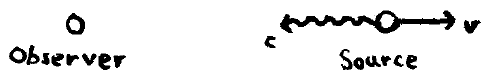
\includegraphics[scale=0.6]{Draw/lec4_7.png}
\end{center}
\caption{Relativistic Doppler effect}
\label{fig:lec4_7}
\end{figure}

In the reference frame of the source, the observer is moving away with speed $v$. The time $\Delta t_{\rm em}$ elapsed between the arrival of two successive wave crests equals the distance between the crests (which is $\lambda_{\rm em}$, the wavelength of the emitted wave) divided by relative velocity between the wave and the observer. That is
\begin{equation}
\Delta t_{\rm em}=\frac{\lambda_{\rm em}}{c-v}.
\end{equation}
In the reference frame of the observer this time is shorter due to the relativistic time dilation; see eq.\ (\ref{eq:time_dilation}). The observer actually measures
\begin{equation}
\Delta t_{\rm obs}=\Delta t_{\rm em}\sqrt{1-\frac{v^2}{c^2}}.
\end{equation}
Now, the observer measures the light ray to have a speed $c$, by the second postulate of SR. Therefore the wavelength measured by the observer is
\begin{equation}
\begin{split}
\lambda_{\rm obs}&=c\Delta t_{\rm obs}\\
&=c\Delta t_{\rm em}\sqrt{1-\frac{v^2}{c^2}}\\
&=\frac{c}{c-v}\sqrt{1-\frac{v^2}{c^2}}~\lambda_{\rm em}.
\end{split}
\end{equation}
Rearranging this equation we obtain
\begin{equation}
\begin{split}
\frac{\lambda_{\rm obs}}{\lambda_{\rm em}}&=\frac{\sqrt{1-\frac{v^2}{c^2}}}{\left(1-\frac{v}{c}\right)}\\
&=\frac{\sqrt{\left(1+\frac{v}{c}\right)\left(1-\frac{v}{c}\right)}}{\left(1-\frac{v}{c}\right)}\\
\end{split}
\end{equation}
\begin{equation}
\Rightarrow~~~~~~\frac{\lambda_{\rm obs}}{\lambda_{\rm em}}= \sqrt{\frac{1+\frac{v}{c}}{1-\frac{v}{c}}}.
\end{equation}
This is the expression of the relativistic Doppler effect for the case in which the source and the observer are moving away from each other. Notice that the right hand side is larger than 1, meaning that $\lambda_{\rm obs}>\lambda_{\rm em}$. This means that, to the observer, the source (a galaxy for instance) looks as if it were emitting light with larger wavelength than it actually is. The source looks ``more red'' to the observer. We say in this case that the light from the source is {\it redshifted}. Quantitatively, the redshift $z$ of the source is defined as
\begin{equation}
z=\frac{\lambda_{\rm obs}-\lambda_{\rm em}}{\lambda_{\rm em}}.
\end{equation}
Notice that by measuring the redshift of an object we can deduce the velocity at which it is receding from us. If the velocity of the object is small compared to the speed of light, so that $v/c\ll1$, we can approximate
\begin{equation}
\sqrt{\frac{1+\frac{v}{c}}{1-\frac{v}{c}}}\approx 1+\frac{v}{c}.
\end{equation}
Then the redshift will be approximately given by
\begin{equation}
z=\frac{\lambda_{\rm obs}}{\lambda_{\rm em}}-1\approx \frac{v}{c}.
\end{equation}
The relation between redshift and velocity is thus very simple in the nonrelativistic case; if we know $z$, then $v\approx cz$.

\par\vspace{\baselineskip}

{\bf Exercise.} Show that, in the general case (i.e.\ without assuming $v\ll c$), the velocity in terms of the redshift is given by the formula
\begin{equation}
\frac{v}{c}=\frac{(z+1)^2-1}{(z+1)^2+1}.
\end{equation}

\par\vspace{\baselineskip}

\subsubsection{Hubble's law}

Hubble's observation that the universe is expanding was based on the independent measurements of the redshift and distance of several nearby galaxies. What he found is that the redshift of a galaxy is directly proportional to its distance, a relation known as Hubble's law:
\begin{equation}
z=\frac{H_0}{c}d.
\end{equation}
In this equation $d$ is the distance to the galaxy, $c$ is the speed of light, and $H_0$ is the Hubble constant. The currently accepted experimental value is
\begin{equation}
H_0=0.71\pm 0.03~{\rm km~s^{-1}~Mpc^{-1}}.
\end{equation}
Recall that for small redshifts we can approximate $z\approx v/c$, so that in this case Hubble's law reduces to
\begin{equation}
v\approx H_0 d.
\end{equation}
What this equation says is that galaxies are moving away from us at a speed proportional to their distance. One may think that this statement contradicts the cosmological principle, since it seems to suggest that the Earth is some sort of special point from which all galaxies are receding. We will next show that this is not true; we will see that Hubble's law and the cosmological principle are perfectly consistent.

Fig.\ \ref{fig:lec4_8} shows three galaxies forming a triangle with sides $r_{12}(t)$, $r_{23}(t)$, and $r_{31}(t)$. If the expansion of the universe is to preserve the homogeneity of space, then the shape of the triangle must not change. This means that the sides of the triangle must change with time at the same rate; this statement can be written as
\begin{equation}
\begin{split}
r_{12}(t)&=a(t)r_{12}(t_0),\\
r_{23}(t)&=a(t)r_{23}(t_0),\\
r_{31}(t)&=a(t)r_{31}(t_0).\\
\end{split}
\end{equation}
Here $t_0$ is the present time, and $a(t)$ is a function known as the {\it scale factor}. It is a monotonically increasing function of $t$ (if we assume that the universe is expanding), and by definition has the value $a(t_0)=1$ today.
\begin{figure}[ht]
\begin{center}
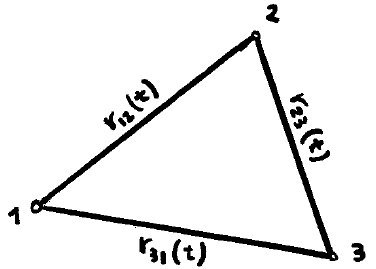
\includegraphics[scale=0.6]{Draw/lec4_8.png}
\end{center}
\caption{Hubble's law and the cosmological principle}
\label{fig:lec4_8}
\end{figure}

From the point of view of galaxy 1, galaxies 2 and 3 are moving away with velocities
\begin{equation}
\begin{split}
v_{12}(t)&=\frac{dr_{12}(t)}{dt}=\frac{da(t)}{dt}r_{12}(t_0)=\frac{\dot{a}}{a}r_{12}(t),\\
v_{31}(t)&=\frac{dr_{31}(t)}{dt}=\frac{da(t)}{dt}r_{31}(t_0)=\frac{\dot{a}}{a}r_{31}(t),\\
\end{split}
\end{equation}
where we introduced the notation
\begin{equation}
\dot{a}(t)\equiv \frac{da(t)}{dt}.
\end{equation}
Let us also define the {\it Hubble parameter}
\begin{equation}
H(t)\equiv \frac{\dot{a}(t)}{a(t)},
\end{equation}
which allows us to write the velocities $v_{12}$ and $v_{31}$ as
\begin{equation}
\begin{split}
v_{12}(t)&=H(t)r_{12}(t),\\
v_{31}(t)&=H(t)r_{31}(t).
\end{split}
\end{equation}
If we evaluate these formulas at $t=t_0$ (the present time), we find
\begin{equation}
\begin{split}
v_{12}(t_0)&=H_0 r_{12}(t_0),\\
v_{31}(t_0)&=H_0 r_{31}(t_0),
\end{split}
\end{equation}
where we have identified $H_0\equiv H(t_0)$, which says that the Hubble constant is simply the present value of the Hubble parameter. With this identification we see that these formulas reproduce Hubble's law for galaxy 1, since they state that galaxies 2 and 3 are receding from galaxy 1 at velocities proportional to their distances. But now we could repeat exactly the same analysis for galaxies 2 and 3, and find that Hubble's law also holds for them (and with the same proportionality constant $H_0$). We conclude from this argument that Hubble's law is consistent with an expansion of the universe that preserves homogeneity and isotropy. There is no violation of the cosmological principle here: just as we see other galaxies moving away from us, the inhabitants of any of these likewise see other galaxies receding from them.

Fig.\ \ref{fig:lec4_9} shows a more recent version of the graph used by Hubble to determine his expansion law. Each dot in the graph represents a galaxy, and one can clearly observe a linear relation between velocity and distance. An important observation, however, is that Hubble's law is only an approximate law, as can be seen from the fact that the dots in the graph do not follow a perfect straight line. This deviation from a ``perfect Hubble's law'' does not happen, of course, because the expansion of the universe is irregular (which would contradict the cosmological principle), but because of the {\it peculiar motion} of the galaxies. The peculiar motion is the motion that occurs due to the gravitational attraction of nearby galaxies, and has nothing to do with the expansion of the universe. For example, the Andromeda galaxy and the Milky Way are not moving away from each other, but they are actually moving closer due to the gravitational attraction that exists between them.
\begin{figure}[ht]
\begin{center}
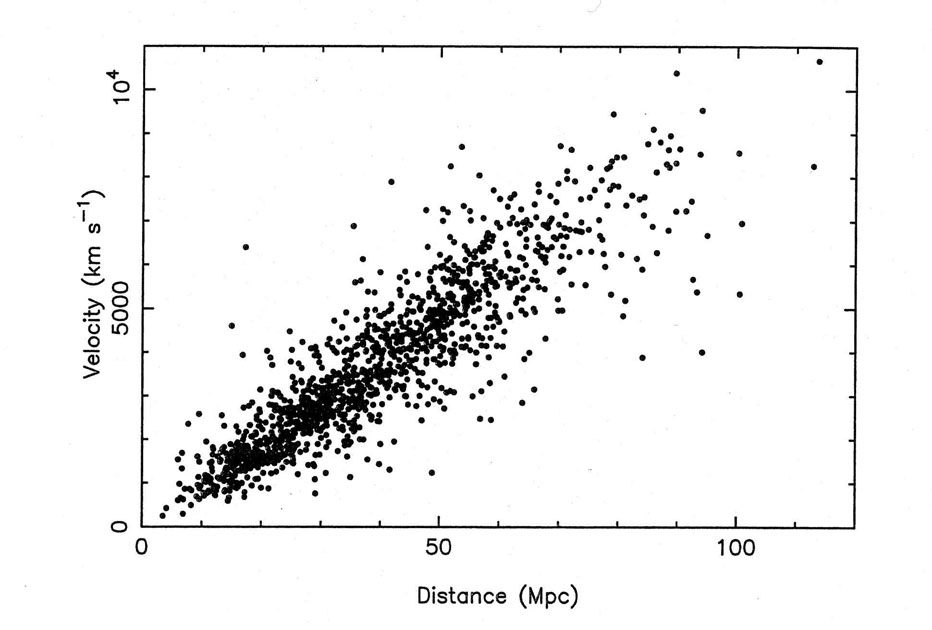
\includegraphics[scale=0.4]{Draw/lec4_9.png}
\end{center}
\caption{Hubble's law (Image credit: J. Imamura, University of Oregon)}
\label{fig:lec4_9}
\end{figure}

\subsubsection{The Big Bang}

If we watch the history of the universe running backward in time, we would see all the galaxies approaching each other. Then, if we assume that the universe has always been expanding, there must have been a time in the past when all particles were infinitely close to each other. In this picture, the universe was born from a state of infinite temperature and density, a state known as the Big Bang.

Consider two galaxies separated today by a distance $d$ and moving away from each other with a speed $v$. Then, by Hubble's law, $v=H_0 d$. Let us assume that the two galaxies have been always moving (relative to each other) with the same speed $v$. The time elapsed since the moment in which they were in contact is then
\begin{equation}
\begin{split}
t_0&=\frac{d}{v}=\frac{d}{H_0 d}=\frac{1}{H_0}\approx 14\times10^9~\mathrm{years}.
\end{split}
\end{equation}
We find that, under this assumption of constant expansion rate, the age of the universe would be roughly 14 billion years.\footnote{The constant $1/H_0$ is sometimes referred to as the Hubble time.} There are, however, two important caveats to this argument. First, $H(t)$ is a function of time, meaning that the expansion rate has not been always the same. How do we even know that the universe has always been expanding? Second, we have stressed above that the expansion of the universe is a large-scale effect; on small scales, the local interactions between bodies always dominate over the Hubble expansion. How do we know then that Hubble's law holds at the early times when the universe was very dense? To answer these questions we need to use GR. Specifically, we need to learn how to describe our universe by means of a metric, and then apply the Einstein equations to find how the scale factor $a(t)$ evolves in time. This will be the subject of the next lecture.


\chapter{The Friedmann model of the universe}
After spending some time mastering the physical and mathematical tools we need (namely special and general relativity), now we are finally ready for a first approach to the study of modern cosmology; what we will examine in this section is the so called Friedmann model of the universe, which is the simplest model current observations suggest about the cosmos on its largest scales. Observations of the uniformity of the Cosmic Microwave Background (CMB) (see Figure \ref{cmb})and of the redshift of galaxies, already treated in the previous chapter, suggest that, at a first apporximation, our observable universe can be modeled as a uniform expanding ball, filled by some homogeneous fluid that triggers the expansion according to the rules of general relativity. We will be a lot more precise in the following paragraphs.

\begin{figure}
\begin{center}
\includegraphics[scale=0.5]{Draw/wmap}
\label{}
\end{center}
\caption{A picture of the temperature Cosmic Microwave Background across the sky, from the experiment WMAP: the fluctuations in temperature from red to blue spots have a relative magnitude $\delta T/T\sim 10^{-5}$.  Credit for the image \url{http://apod.nasa.gov/apod/ap030212.html}}
\label{cmb}
\end{figure}

\section{A uniform ball} 
As stated before, the uniformity of the temperature of the CMB (with fluctuations of relative order $10^{-5}$), measured all across the sky, suggests that our special observation point, Earth, has no special role at all in the universe physical picture: this can be stated as the so called \textit{cosmological principle}, which says that \textit{every observer in the universe} (at rest), will experience the same cosmology, and will get the same results in any observational experiment. This also mean, that all all observers \textit{at rest} (we will explain what this means in the following), will agree on the measurement of time, and we will call this common time reference $t$ ($t=0$ being the beginning of the universe, the Big Bang). In each one of these \textit{at rest} reference frames, we can hence say that our metric will be something like
\begin{equation}
\label{frwsymb}
ds^2=-c^2dt^2+ds_3^2
\end{equation}    
Where $ds_3^2$ is the spacial part of the metric (that involving $dx,dy,dz$) and depends on the spatial geometry of our universe, i.e. on how we measure \textit{spatial} distances. The fact that the universe is homogeneous, as suggested by observations, tells us that $ds_3^2$ cannot be arbitrary, but must satisfy this homogeneity assumption. You can convince yourselves that there are only three possible types of spatial metric that satisfy this requirement, namely a flat metric with curvature $k=0$, a positively curved metric with constant curvature $k=1/R^2$ or a negatively curved metric with constant curvature $k=-1/R^2$. Note that if we want do describe a curved universe, we must specify a curvature scale length, $R$ (the ''radius of curvature'') as pointed out in chapter 2. 
\subsection{The flat case}
If the universe were flat, with no curvature, then the spatial metric would just be the one you are already familiar with in ordinary euclidean space, in which we measure distances with the pythagorean theorem (in coordinates $(x,y,z)$)
\begin{equation}
ds_3^2=dx^2+dy^2+dz^2
\end{equation}
We usually like to use spherical coordinates $(r,\theta,\phi)$, in which the metric becomes that of equation (\ref{metspher})
\begin{equation}
ds_3^2=dr^2+r^2(d\theta^2 + \sin^2{\theta}d\phi^2)
\end{equation}
\subsection{Positive curvature: the sphere case}
If our universe were positively curved, we would model it as a sphere of radius $R$, because this is the only space that has constant positive curvature; the only difference from what we already saw, is that this sphere would be three dimensional (a so called 3-sphere, or $S^3$), not two dimensional as the spheres we saw in chapter 2. How do we model such a sphere? A 3-sphere is a three dimensional subset of a 4 dimensional eucliudean space with coordinates $(x,y,z,w)$; this subset has to satify the constraint
\begin{equation}
x^2+y^2+z^2+w^2=R^2
\end{equation}
Since on this four dimensional space we measure distances with the usual euclidean metric 
\begin{equation}
\label{positive4d}
ds_4^2=dx^2+dy^2+dz^2+dw^2
\end{equation}
If this is how we measure distances on all space,we want to understand on how this four dimensional metric translates into a three dimensional metric on our 3-sphere; this is easily done in spherical coordinates $(r,\theta,\phi)$, which give us a very good parametrization of the sphere (notice that we use only three coordinates because the sphere is a three dimensional subset of this four dimensional space) 
\begin{displaymath}
\left \{ \begin{array}{l}x=r\sin{\theta}\cos{\phi} \\ 
y=r\sin{\theta}\sin{\phi} \\ 
z=r\cos{\theta} \\
w= \sqrt{R^2-r^2} \end{array}  \right.  
\end{displaymath} 
If you calculate all the derivatives and express $(dx,dy,dz,dw)$ in terms of $(dr,d\theta,d\phi)$ and plug the results in (\ref{positive4d}), you will obtain an induced three dimensional metric in the form
\begin{equation}
\label{poscurv}
ds_3^2=\frac{dr^2}{1-\left(\frac{r}{R}\right)^2} + r^2(d\theta^2 + \sin^2{\theta}d\phi^2)
\end{equation}
Note that this metric reduces to the flat one when $R$ becomes very big: this was also expected given the considerations in chapter 2
\subsection{Negative curvature: the hyperboloid case}
The negative curvature case is more complicated to think about, because it's not as easy to visualize as the sphere one: in this case we always start from a four dimensional space with coordinates $(x,y,z,w)$, in which we consider a subset given by the constraint
\begin{equation}
x^2+y^2+z^2-w^2=-R^2
\end{equation}
One mathematically can show that this space has constant negative curvature $-1/R^2$ if we measure distances on it according to the four dimensional metric 
\begin{equation}
ds_4^2=dx^2+dy^2+dz^2-dw^2
\end{equation}
Notice the minus sign on the last addend, which is \textit{crucial}; as in the sphere case, we wish to see what is the induced metric $ds^2_3$ on this three dimensional subset (which we call 3-hyperboloid); again, it is useful to work in spherical coordinates, that suggest us a good parametrization
\begin{displaymath}
\left \{ \begin{array}{l}x=r\sin{\theta}\cos{\phi} \\ 
y=r\sin{\theta}\sin{\phi} \\ 
z=r\cos{\theta} \\
w= \sqrt{R^2+r^2} \end{array}  \right.  
\end{displaymath}
If you go through the same steps as for obtaining (\ref{poscurv}), this time you would obtain something like
\begin{equation}
\label{negcurv}
ds_3^2=\frac{dr^2}{1+\left(\frac{r}{R}\right)^2} + r^2(d\theta^2 + \sin^2{\theta}d\phi^2)
\end{equation}
To summarize, the homogeneity of the universe, suggested by observations, tells us that the spatial part of the metric that describes it must have necessarily the form 
\begin{equation}
\label{gencurv}
ds_3^2=\frac{dr^2}{1-k\left(\frac{r}{R}\right)^2} + r^2(d\theta^2 + \sin^2{\theta}d\phi^2)
\end{equation}
And there are only three possibilities for $k$, which has to be constant and be chosen between 0(flat case), 1(positive curvature case) or -1 (negative curvature case). Sometimes it's useful to introduce another parametrization of the radial coordinate $r$, in the following way: 
\begin{displaymath}
\left \{ \begin{array}{l}k=1\rightarrow r=R\sin{\left(\frac{\chi}{R}\right)} \\ 
k=0\rightarrow r=\chi \\ 
k=-1 \rightarrow r=R\sinh{\left(\frac{\chi}{R}\right)} \\
 \end{array}  \right.  
\end{displaymath}
So that the spatial metric becomes 
\begin{equation}
ds_3^2=d\chi^2+s^2_k(\chi)(d\theta^2 + \sin^2{\theta}d\phi^2)
\end{equation}
where the curvature is encoded in the angular weight function $s_k(\chi)$ that takes one of the following forms 
\begin{displaymath}
s_k(\chi)=\left \{ \begin{array}{l}k=1\rightarrow R\sin{\left(\frac{\chi}{R}\right)} \\ 
k=0\rightarrow \chi \\ 
k=-1 \rightarrow R\sinh{\left(\frac{\chi}{R}\right)} \\
 \end{array}  \right.  
\end{displaymath}
We will examine the physical consequences of this geometrical description in the following paragraph. 

\section{The expansion of the universe}
Now that we know how the universe's homogeneity constrains the spatial part of the metric in (\ref{frwsymb}), we are ready to add another ingredient to our physical model of the universe: the expansion. This final ingredient will ultimately explain the redshift phenomenology that we see in all our observations. To understand how the expansion works, you have to model again the universe as a ball: imagine that we live on the surface of this ball (or balloon) and that this ball gets inflated by some kind of mechanism. What will we experience as a result of this expansion? You may recall what you learned at the end of last chapter, but let's go over this again briefly. 
\begin{figure}
\begin{center}
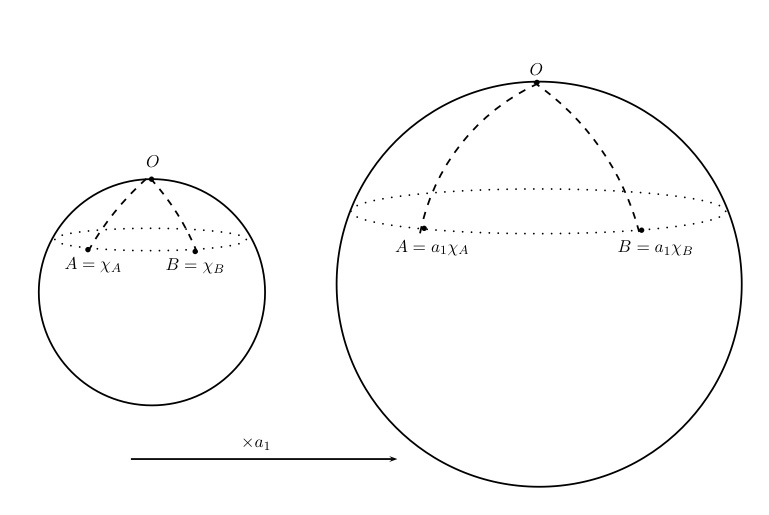
\includegraphics[scale=0.8]{Draw/expansion.png}
\label{}
\end{center}
\caption{A universe-balloon that inflates, growing its size by a factor $a_1$}
\label{expansion}
\end{figure}
Consider the example in Figure \ref{expansion}: if we choose a spherical coordinate system $(\chi,\theta,\phi)$ centered in $O$ ($\chi=0$ corresponds to $O$), we choose two points at distances $\chi_A$ and $\chi_B$ from $O$: if now we inflate the balloon, and its size grows by a factor $a_1$, then all the distances measured on the balloon will grow by the same amount. That is to say, on the inflated balloon, the points $A$ and $B$ will find themselves at a physical distance $a_1\chi_A$ and $a_1\chi_B$ from $O$; nevertheless, we can still identify the points $A$ and $B$ on the inflated balloon, by their \textit{comoving distances} $\chi_A$ and $\chi_B$, provided that we know the \textit{scale factor} $a_1$, that allows us to compute the \textit{physical distances} $\chi_{phys}=a_1\chi$. We will picture our expanding universe in an exacly analogous way: we choose $O$ as our observation point, Earth, and we choose a spherical coordinate system $(\chi,\theta,\phi)$ centered on us (this choice is arbitrary, but 
there's nothing special in it, as the cosmological principle dictates, it is only a matter of convenience): we intend the coordinate $\chi$ as a radial comoving distance, which can be converted into a physical radial distance, if we know the scale factor $a$ of the universe. The statement that the universe expands, means that the scale factor $a(t)$ depends on time, and grows, meaning that physical distances between objects grow as well ($\chi_{phys}=a(t)\chi$); this description gives us a good definition of observers \textit{at rest}: an observer is at rest with the expansion of the universe if its comiving coordinate $\chi$ doesn't change with time. Note that, even if two galaxies are at rest (their comoving distance is the same), their physical distance grows indeed, because it gets multiplied by $a(t)$. This means that the geometry of our homogeneous, expanding universe will be encoded in a metric in the form 
\begin{equation}
\label{frw}
ds^2=-c^2dt^2+a^2(t)\left[d\chi^2+s^2_k(\chi)(d\theta^2 + \sin^2{\theta}d\phi^2)\right]
\end{equation}  
or 
\begin{equation}
g_{\mu\nu}[k,a(t)]=
\begin{pmatrix}
-c^2 & 0 & 0 & 0 \\
0 & a^2(t) & 0 & 0 \\
0 & 0 & a^2(t)s_k^2(\chi) & 0 \\
0 & 0 & 0 & a^2(t)s_k^2(\chi)\sin^2{\theta}
\end{pmatrix}
\end{equation}
This form of the metric is called \textit{Friedmann-Roberson-Walker} metric, from the name of the physicists who first proposed it: this is the most general metric we can write down for an expanding, homogeneous universe. Once we specify the matter content of the universe, encoded in the stress energy tensor $T_{\mu\nu}$, we can plug the metric in the Einstein equation
\begin{equation}
\label{einfried}
G_{\mu\nu}[k,a(t)]=\frac{8\pi G}{c^4}T_{\mu\nu}
\end{equation}
which will translate in a differential equation for $k$ and $a(t)$; we can solve this equation and find the time dependence of the scale factor $a(t)$ to see how fast the universe expands in various scenarios (remember that in this differential equation, which by the way is called \textit{Friedmann equation}, will also make appearence $R$, our comoving curvature scale); before going into these details, however, let's examine some of the important features of a metric in the form (\ref{frw})
\subsection{Cosmological redshift}
What we will try to do in this section, is convince ourselves that a metric in the form \textit{Friedmann-Robertson-Walker} naturally explains the redshift of galaxies that we see in our observations: you already encountered this concept in the previous lecture, interpreting it as a dopplershift; here we will interpret this effect under a slightly different perspective. Consider a light source (for example a galaxy) at a comoving distance $\chi_E$ from us, as in Figure \ref{redshift}
\begin{figure}
\begin{center}
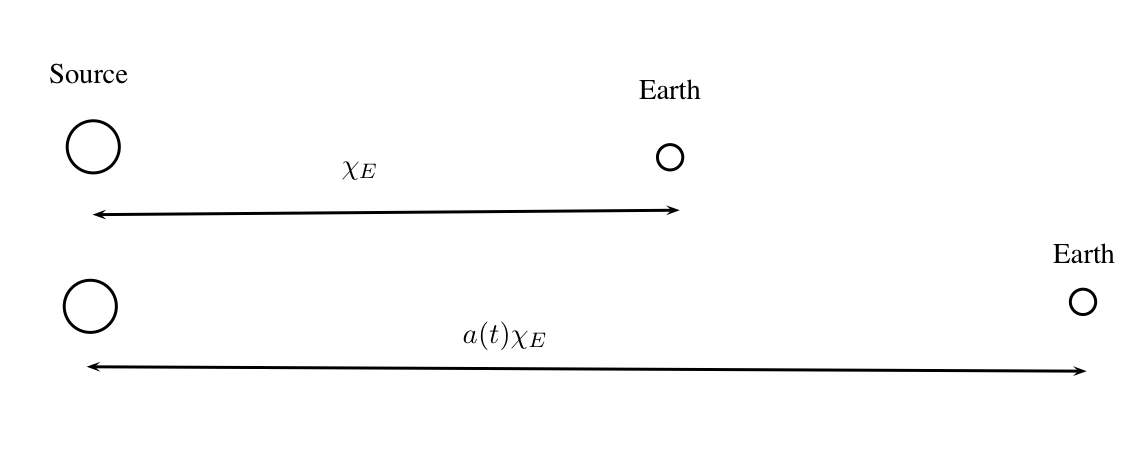
\includegraphics[scale=0.8]{Draw/redshift.png}
\label{}
\end{center}
\caption{A picture explaining cosmological redshift}
\label{redshift}
\end{figure}
This galaxy will emit light at a frequency $f_S$; if both we and the galaxy are at rest with the expansion, the comoving distance between us $\chi_E$ will remain constant, but nevertheless the galaxy will recede from us because the physical distance will grow as $a(t)\chi_E$: this will have the consequence that the light that we receive on earth will have a lower frequency $f_E$.  Now, remember emember that light travels always along null geodesics ($ds^2=0$), so if we have to follow the path of a photon $\chi(t)$ from the galaxy ($\chi=\chi_E$) to us ($\chi=0$), this path must satisfy $ds^2=0$ or $a(t)d\chi=-cdt$. Suppose a photon is emitted from the galaxy at time $t_S$ and is received at earth at a subsequent time $t_E=t_E(t_S)$. It is then true that 
\begin{equation}
\label{comdis}
\chi_E=\int_E^Sd\chi=c\int_{t_S}^{t_E(t_S)}\frac{dt}{a(t)}
\end{equation}
Since the number of photons emitted should be the same of the number of photons receive on earth, it must be true that $f_Edt_E=f_Sdt_S$, which will immediately tell us that if we define a \textit{redshift parameter} associated with our galaxy (that quantifies the difference between emitted and received light frequency) in the obvious way
\begin{equation}
z\equiv \frac{f_S-f_E}{f_E}
\end{equation}
then the following relation must hold
\begin{equation}
z=\frac{dt_E}{dt_S}-1
\end{equation}
Now take equation (\ref{comdis}), differentiate it with respect to $t_S$ taking into account that the comoving distance is constant $\frac{d\chi_E}{dt_S}=0$ to get $\frac{dt_E}{dt_S}=\frac{a(t_E)}{a(t_S)}$. If we call $z_S$ the redshift parameter of our galaxy, which is the quantity that we measure in observations (looking at the shift in the galaxy emission spectra), we immediately get
\begin{equation}
1+z_S=\frac{a(t_E)}{a(t_S)}
\end{equation}
This tells us a fact of the uttermost importance: if by convention we set the scale factor today (at $t_E$) as unity ($a(t_E)=1$), then we see that $a(t_S)=\frac{1}{1+z_S}$, that is to say the redshift of our galaxy is a measure of the scale factor of the universe at the time when the light was emitted. If we knew the time dependence $a(t)$ (for which we have to solve Einstein's equation), then redshift $z$ would provide us with a direct measure of the age of the universe $t(z)$ at which the light that we see was emitted
\subsection{Redshift as a measure of distance}
It happens that, one we exploit at full the properties of the metric (\ref{frw}), we discover that redshift is not only a measure of time, but also of the physical distance $d_E$ between us and the galaxy of which we measure the redshift. We have that
\begin{equation}
d_S=a(t_E)\chi_E=a(t_E)\int_{t_S}^{t_E}\frac{cdt}{a(t)}=\int_{z_S}^0\frac{c}{a(z)}\frac{dt}{dz}dz
\end{equation}
Now take into account that $\frac{dz}{dt}=-\frac{\dot{a}(t)}{a^2(t)}a(t_E)$, and define the \textit{Hubble parameter} as 
\begin{equation}
H(t)=\frac{\dot{a}(t)}{a(t)}
\end{equation}
to get
\begin{equation}
\label{distanceredshift}
d_E(z_S)=\int_0^{z_S}\frac{c}{H(z)}dz
\end{equation}
Note that the Hubble parameter $H(t)$ has units 1/time, and is a measure of the expansion rate of the universe; moreover, it is completely insensible to the convention we used $a(t_E)=1$. Its value today $H(t_E)=H_0$ is called \textit{Hubble constant}, and is measured to be $H_0=100h\,\mathrm{km}\,\mathrm{s}^{-1}\mathrm{Mpc}^{-1}$ with $h\sim 0.7$. Note also that, in order to convert redshift $z$ in a measure of time and distance, we first need to solve the Friedmann equation to get the dependency $a(t)$, which in the end depend on the matter content of our universe. We will get to this in the next section. 

\section{The Friedmann equation}
What we want to do in this section is mainly find a way to compute the evolution of the scale factor $a(t)$; as pointed out in the previous paragraphs, in order to do that we need to know the matter content of the universe (what is it made of) and then solve Einstein's equation (\ref{einfried}) for $a$. Before going into this, though, we need to see how this equation looks like when we write it down in terms of $a$ and $\dot{a}$.
\subsection{The matter content of the universe}
As we pointed out before, we model our universe, at a first approximation, as a uniform inflating ball filled of some homogeneous fluid of density $\rho$: in the previous section we focused on what are the physical and observational consequences of this expansion, now we want to focus on \textit{the meachanism} that triggers this size growth. It turns out that, according to general relativity, what causes the expansion is the universe itself, or better, the matter it is made of. This homogeneous fluid that permeates our balloon might have different components that have different characteristics and have different physical consequences. We describe these different components in term of their energy momentum tensor $T_{\mu}^{\nu}$; we distiguish two main contributions to the overall energy budget:
\begin{itemize}
\item Ordinary matter and dark matter: these kind of components are described by perfect fluids of uniform density $\rho$ and pressure $P$, which are connected by the so called \textit{equation of state} $P=w\rho c^2$. The number $w$ specifies the type of matter we are considering; over 75\% of the overall matter budget in our universe is made by \textit{dark matter}, which does not interact with light and hence cannot be seen directly in observations, and today is only indirectly detected observing its gravitational effects. The true nature of dark matter is still unknown (we will get to this towards the end of the course). All this matter content is described by an energy momentum tensor in the form 
\begin{equation}
T_{\mu,M}^\nu=(P+\rho c^2)U_\mu U^\nu + P\delta_\mu ^ \nu
\end{equation} 
Where $U^\mu$ is the 4-velocity of the fluid elements (in units of $c$) and, if this fluid is homogeneous and at rest with the expansion, then this 4-velocity is forced to have the form $U^\mu=\left(\frac{dt}{dt},\frac{d\chi}{dt},\frac{d\theta}{dt},\frac{d\phi}{dt}\right)=(1,0,0,0)$
\item Dark energy: the presence of this component in the overall energy budget is probably one of the most tricky unsolved mysteries in science. Nevertheless its presence is required by current observation of the accelerated expansion of the universe; its energy momentum tensor can be written in the form
\begin{equation}
T_{\mu,DE}^\nu=-\frac{\Lambda c^4}{8\pi G}\delta_\mu^\nu
\end{equation}
With $\Lambda$ a suitable constant with units length$^{-2}$; why immediately see why this kind of energy source is really particular. It can be indeed thought as some kind of fluid with equation of state $P=-\rho c^2$, i.e. a fluid with \textit{negative} pressure: if ordinary and dark matter exert a positive pressure telling the universe to stop expanding (exerting positive gravity), this kind of dark energy tells us exacly the opposite, it exerts a negative gravity that pushes out and accelerates the expansion of the universe! Moreover, current observations of the CMB and galaxy surveys tell us that not only this weird dark energy is there, but it makes up for more that 70\% of the overall energy budget. The natural question we may ask then is: where does it come from? And the answer is again ''we don't know''; current observations today measure $\Lambda \approx 10^{-52}\mathrm{m}^{-2}$, which translates in a physical length scale of $1/\sqrt{\Lambda}\approx 10^{26}\mathrm{m}\approx 3\mathrm{Gpc}$. Beside 
the pure coincidence fact that this length scale equals the size of the observable universe today, this length scale is extremely mysterious: there is no current physical theory, neither general relativity nor the standard model in which this length scale emerges naturally. The origin of this \textit{cosmological constant} $\Lambda$ is hence still unknown. 
\end{itemize}
\subsection{The evolution equation} 
If we plug in $T_{\mu,M}^\nu$ and $T_{\mu,DE}^\nu$ in the right hand side of (\ref{einfried}) and work out the proper differential calculations, we end up with a differential equation for $a(t)$, that takes the remarkable form 
\begin{equation}
\label{friedmanneq}
\left(\frac{\dot{a}(t)}{a(t)}\right)^2=\frac{8\pi G}{3}\rho[a(t)]-\frac{kc^2}{R^2a^2(t)}+\frac{\Lambda c^2}{3}
\end{equation}
This is a proper differential equation for $a(t)$ that takes the name of \textit{Friedmann equation} and, as promised, ties together the energy properties ($\rho$ and $\Lambda$) and the geometrical properties (the scale factor $a$ and the curvature scale $Ra$) on our physical system. This equation can in principle be solved to get the explicit dependence of $a$ in terms of $t$, except that we still don't know how the fluids' densities depend on the size of the universe $a$. This will be our next goal
\subsection{A little bit of thermodynamics}
To understand how the densities of the various matter components scale with $a$ we have to apply nothing more than the first principle of thermodynamics, which says that the change of energy $dE$ of a physical system is given by the heat that flows in $dQ$ minus the work done by the system $dW=PdV$, being $V$ and $P$ the volume and pressure of the system: $dE=dQ-PdV$. Since in our case the universe is an isolated system, there is no heat flowing in nor flowing out $dQ=0$ and we can use $E=\rho a^3$ and $V=a^3$ to get
\begin{equation}
d(\rho a^3)=-Pd(a^3)=-w\rho d(a^3)
\end{equation}
For a component with equation of state $w$; working out the calculations, this equation can be simplified into 
\begin{equation}
\frac{d\rho}{\rho}=-3(1+w)\frac{da}{a}
\end{equation}
Which in the end leads to a scaling 
\begin{equation}
\rho(a)=\rho(a_0)\left(\frac{a}{a_0}\right)^{-3(1+w)}
\end{equation}
It turns out that the total matter budget of the universe can be divided into two main classes:
\begin{itemize}
\item ''Cold'', non relativistic matter, made of particles which move with speeds $v\ll c$; today, all ordinary matter (electrons, protons, nuclei, atoms) as well as dark matter belong to this category. For this kind of matter, one can estimate the equation of state index as 
\begin{equation}
w=\frac{P}{\rho c^2}=\frac{k_B T}{mc^2}\approx \left(\frac{v}{c}\right)^2\ll 1
\end{equation}
Where $T$ and $m$ are respectively the temperature and particle mass associated with this particular component: for the sake of this lecture we can safely set $w=0$ for this ''cold'' matter and obtain a scaling $\rho_c(a)\propto a^{-3}\propto (1+z)^3$
\item ''Hot'', relativistic matter, made of particles which move with speeds close to the speed of light $v\sim c $ : both photons (massless) and neutrinos (which have very little mass) belong to this category. Relaticistic thermodynamics tells us that this "hot" matter can be described in terms of an equation of state index of $w=1/3$ and hence the density for these particular fluid components should scale as $\rho_h(a)\propto a^{-4}\propto (1+z)^4$
\end{itemize}
\subsection{Some particular solutions to the Friedmann equation: how to measure the age of the universe}
We have seen in the previous section that some of the components our universe is made of exibit a simple scaling in their density $\rho(a)\propto a^{n}$. Suppose we wish to solve the Friedmann equation (\ref{friedmanneq}) assuming our universe is flat ($k=0$ or $R=\infty$), contains no dark energy ($\Lambda = 0$, this is unrealistic but helps us make some estimates) and contains only one fluid component described by an equation of state index $w$ (which in real cases can be 0 or 1/3). Then our Friedmann equation will simplify enormously and reduce to 
\begin{equation}
\left(\frac{\dot{a}(t)}{a(t)}\right)^2=\frac{8\pi G\rho_0}{3a_0^n}[a(t)]^n
\end{equation}
Since the choice of $a_0$ is arbitrary, this equation has no natural timescale built in, and hence we seek a solution in the form $a(t)=Ct^\lambda$, with $C$ and $\lambda$ some constant numbers. We have little interest in the normalization constant $C$, since it can always be set to 1 redefining the scale factor at some particular time (as we did with our convention $a(t_E)=1$), what we are really interested in is the exponent $\lambda$, which is the one that tells us how fast the universe expands. Matching the powers of $t$ on the left and right hand side of the equation above gives us the relation $-2=\lambda n$ and hence $\lambda=-2/n$, and an overall solution
\begin{equation}
a(t)=a(t_E)\left(\frac{t}{t_E}\right)^{\frac{2}{3(1+w)}}
\end{equation}
Which gives us the dependencies $a(t)\propto t^{2/3}$ if only cold matter is present and $a(t)\propto t^{1/2}$ if only hot matter is present. Moreover, we can express the Hubble constant today as
\begin{equation}
H_0=\frac{\dot{a}(t_E)}{a(t_E)}=\frac{2}{3(1+w)}\frac{1}{t_E}
\end{equation}
If we think about it a little bit, this last equation gives us an expression for the age of the universe today, which is nothing more than $t_E=2/[3(1+w)H_0]$: both in the cold case $w=0$ and in the hot case $w=1/3$ this relation gives us an estimate for the age of the universe $t_E\approx 10$\,Gyr, which is not that far from the number you get if you were to consider the full matter + dark energy + curvature model. 
Let's consider another naive but interesting example: if our universe were to be flat and contain no matter at all, but just dark energy, the friedmann equation would reduce to
\begin{equation}
\frac{\dot{a}(t)}{a(t)}=\sqrt{\frac{\Lambda c^2}{3}}\equiv H_0
\end{equation}
which would have a solution $a(t)=a(t_E)e^{H_0(t-t_E)}$, i.e. would describe an exponential, \textit{accelerated} expansion with $\ddot{a}(t)>0$; compare this to the previous studied case with matter only: you may convince yourselves that these matter only models describe a \textit{decelerated} expansion with $\ddot{a}(t)<0$. That's what dark energy does for us: it pushes out and accelerates our universe's expansion, helping us explain the experimental data we see (which strongly indicate an accelerated expansion). When we consider a more realistic model, a flat universe with both dark matter and dark energy (the so called $\Lambda$CDM model, in which matter makes up for 1/4 and dark energy for 3/4 of the overall energy budget, as observations suggest) we get a more complicated time dependence 
\begin{equation}
\frac{a(t)}{a(t_E)}=\left[\frac{\sinh{\left(\frac{3\sqrt{\Omega_\Lambda}H_0 t}{2}\right)}}{\sinh{\left(\frac{3\sqrt{\Omega_\Lambda}H_0 t_E}{2}\right)}}\right]^{2/3}
\end{equation}
With $\Omega_\Lambda=\frac{\Lambda c^2}{3H_0^2}\approx 0.75$; we'll talk more about this model in the following chapter. For the moment, you can lookup at table \ref{timez} that outlines some of the most important events in the universe's history, with the time-redshift conversion made according to the flat $\Lambda$CDM model

\begin{table}[htdp]
\begin{center}
\begin{tabular}{|c|c|c|} \hline
\textbf{Event} & \textbf{Redshift}$z$ & \textbf{Corresponding time}($\Lambda$CDM) \\ \hline
Big bang & $\infty$ & 0 \\ \hline
Cold and hot matter density is the same & 3200 & $6\cdot 10^4$yr \\ \hline
Decoupling, origin of the CMB & $10^3$ & $3\cdot 10^5$yr \\ \hline
Reionization & $10$ & $0.5$Gyr \\ \hline
Today& 0 & $13$Gyr \\ \hline
\end{tabular}
\end{center}
\caption{Some important event's in the universe's history}
\label{timez}
\end{table}


\chapter{The Friedmann equation and the thermal history of the universe}

In this chapter we continue with the discussion of the Friedmann equation that we started in the previous chapter. In particular, we will see how the presence of dark energy dramatically affects the evolution of the universe at late times. We will then begin the study of the thermal history of the universe. At early times, the particles in the universe form a fluid in thermodynamic equilibrium with a well-defined temperature. This temperature decreases as the universe expands, with the consequence that the properties of this cosmic fluid change in time (hence the name ``thermal history''), and in particular, some particle species decouple from the fluid at certain stages. One of the most important stages is the one in which the photons of the cosmic fluid decouple (when the universe was around $380,000$ years old) and begin to travel freely with no further interactions with other particles. These are the photons that we can observe today in the cosmic microwave background (CMB).

\section{The Friedmann equation (continued)}

\subsection{The FRW metric: summary}

We begin with a summary of the Friedmann-Robertson-Walker (FRW) metric. Recall that the cosmological principle, that is, the experimental fact that the universe is homogeneous and isotropic on large scales, implies that the universe must be described mathematically by the metric
\begin{equation} \label{eq:frw_metric}
ds^2=-c^2dt^2+a(t)^2\left[\frac{dr^2}{\left(1-k\frac{r^2}{R^2}\right)}+r^2\left(d\theta^2+\sin^2\theta d\phi^2\right)\right].
\end{equation}
This is known as the FRW metric. Actually, depending on the value of the parameter $k$, the expression in (\ref{eq:frw_metric}) describes three different spacetimes. For $k=0$ the spacetime has zero spatial curvature,\footnote{By spatial curvature we mean the curvature of the 3-dimensional spaces whose geometry is described by eq.\ (\ref{eq:frw_metric}) with $t=\mathrm{constant}$. In mathematical language, these spaces are called the spatial slices of the spacetime (\ref{eq:frw_metric}).} which implies that two light rays that start traveling parallel to each other will remain parallel. For $k=1$ the spacetime has positive spatial curvature, implying that two light rays that start parallel will eventually converge. Finally, for $k=-1$ the spacetime has negative spatial curvature, and so two light rays that start parallel will eventually diverge. In the cases $k=1$ and $k=-1$, the ``amount'' of curvature is quantified by the {\it curvature radius} $R$; the larger $R$, the less curved the space is. The 
cosmological principle does not tell us what are the values of $k$ and $R$, so they need to be experimentally measured.

The function $a(t)$ is known as the {\it scale factor}.\footnote{The scale factor was introduced in chapter 4, section 4.3.} Recall from chapter 4 that, in any space, the distance between two infinitesimally close points is given by $ds$; if the points are separated by a finite distance then we would simply integrate $ds$. In spacetimes, on the other hand, where we also deal with a time dimension, the distance between two infinitesimally close points (or events) is also given by the spacetime interval $ds$, but with the important condition that the two points must have equal times (that is, the events must be simultaneous); otherwise $ds$ cannot be interpreted as a distance in the usual sense (recall that $ds^2$ does not even need to be positive). For example, in the case of an FRW spacetime the distance $dl$ between two simultaneous events would be given by eq.\ (\ref{eq:frw_metric}) with $t$ constant:
\begin{equation} \label{eq:frw_dist}
dl(t)=a(t)\left[\frac{dr^2}{\left(1-k\frac{r^2}{R^2}\right)}+r^2\left(d\theta^2+\sin^2\theta d\phi^2\right)\right]^{1/2}.
\end{equation}
The important thing to note here is that the distance $dl$ is a function of time because of the presence of the scale factor $a(t)$. The coordinates $(r,\theta,\phi)$ are comoving spherical coordinates.\footnote{Spherical coordinates were introduced in chapter 3, section 3.3.} The name ``comoving'' means that galaxies remain with the same coordinates $(r,\theta,\phi)$ as the universe expands.\footnote{This is an approximation that is valid on large scales. Remember that galaxies have a peculiar motion in addition to the motion due to Hubble's law (see chapter 4), which implies that the coordinates $(r,\theta,\phi)$ for a given galaxy will slightly change in time. This is negligible on large scales, however.} We can think of the grid defined by the coordinates $(r,\theta,\phi)$ to be expanding in time; galaxies have fixed positions on this grid, and therefore fixed values of $(r,\theta,\phi)$. The distances between galaxies, however, are not fixed in time; this is because distances do not only depend on the 
coordinates of the comoving grid, but also on the scale factor $a(t)$, as it is clear from eq.\ (\ref{eq:frw_dist}). Fig.\ \ref{fig:lec6_1} shows two galaxies on the comoving grid (with the coordinate $\theta$ omitted) at two different times; notice that, even though the comoving coordinates of each galaxy remain fixed, the distance between the two increases in time.
\begin{figure}[ht]
\begin{center}
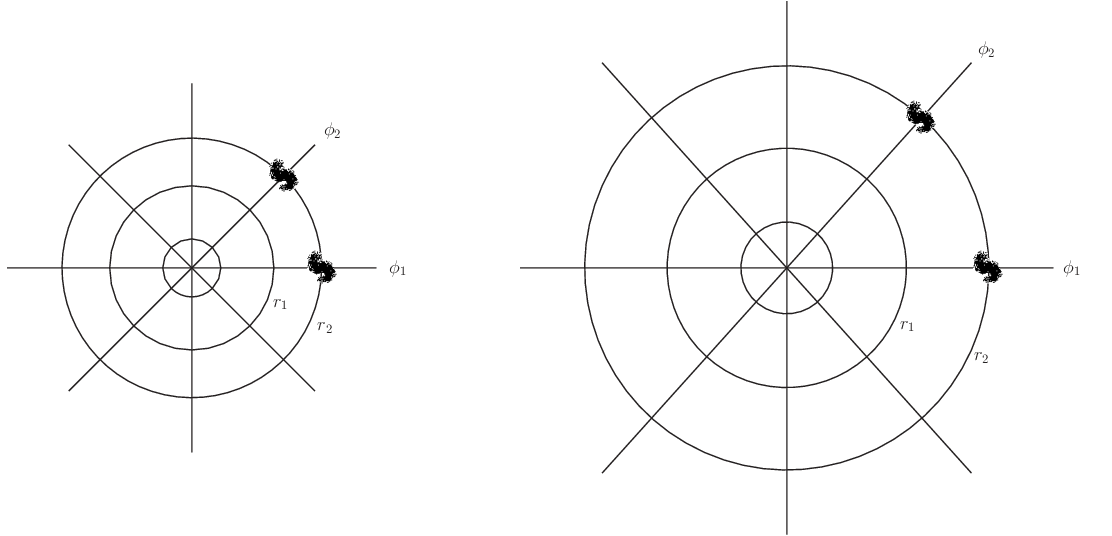
\includegraphics[scale=0.5]{Draw/lec6_1.png}
\end{center}
\caption{Comoving coordinates in the FRW metric}
\label{fig:lec6_1}
\end{figure}

\subsection{The Friedmann equation and the energy content of the universe}

We have learned that distances between objects in a homogeneous and isotropic universe change in time according to the scale factor, and therefore the function $a(t)$ is a direct measure of the expansion of the universe. The next step is to find how $a(t)$ changes in time, for which we need to make use of the Einstein equations. Recall that there are two ingredients in the Einstein equations: the metric (from which the Einstein tensor is constructed) and the energy-momentum tensor. We already have the metric, or more specifically, we have the form of the metric, since we do not know $a(t)$. We also know what is the form of the energy-momentum tensor: on large scales the matter in the universe can be well approximated as a perfect fluid.\footnote{The Einstein equations, the energy-momentum tensor, and perfect fluids were introduced in chapter 4.} With these ingredients the Einstein equations reduce to a simple differential equation that relates the scale factor $a(t)$ to the energy density $\rho(t)$:\footnote{
Notice that in chapter 5 we defined $\rho(t)$ as the {\it mass density} of the fluid, whereas here we adopt the more usual convention of defining $\rho(t)$ as the {\it energy density}. The only difference between the two is a factor of $c^2$.}
\begin{equation} \label{eq:friedmann_eq}
\left(\frac{\dot{a}}{a}\right)^2= \frac{8\pi G}{3c^2}\rho(t)-\frac{kc^2}{R^2a^2}.
\end{equation}
This is known as the {\it Friedmann equation}. We have adopted the notation
\begin{equation}
\dot{a}(t)\equiv \frac{da(t)}{dt}.
\end{equation}
Notice that we have made the assumption that the energy density depends only on time, not on position. This is a consequence of the cosmological principle: since all points in space are equivalent, they all must have the same energy density at any given time. In eq.\ (\ref{eq:friedmann_eq}) $\rho(t)$ denotes the {\it total} energy density, that is, the sum of the energy densities of all the sources present in the universe. There are three main types of sources: matter (with energy density $\rho_m(t)$), radiation (energy density $\rho_r(t)$), and dark energy (energy density $\rho_{\Lambda}$). Thus we can write
\begin{equation}
\rho(t)=\rho_m(t)+\rho_r(t)+\rho_{\Lambda}.
\end{equation}
Notice that the dark energy density $\rho_{\Lambda}$ is independent of time. The nature of dark energy is unknown, but one explanation is that it is an energy contained in the vacuum. Since the vacuum does not care about the expansion of the universe (which is a gravitational effect), the density of dark energy is thought to be constant in time.\footnote{We will say a lot more about dark energy, including some possible explanations, in a later lecture.}

In order to solve the Friedmann equation we need to know how $\rho_m$ and $\rho_r$ depend on the scale factor $a(t)$. In chapter 5 we used a general thermodynamical argument to show that $\rho_m\propto a^{-3}$ and $\rho_r\propto a^{-4}$. To find the constants of proportionality we evaluate at the present time $t_0$ and use that, by definition, $a(t_0)=1$. This gives
\begin{equation}
\begin{split}
\rho_m(t)&= \frac{\rho_m(t_0)}{a(t)^3},\\
\rho_r(t)&= \frac{\rho_r(t_0)}{a(t)^4},\\
\end{split}
\end{equation}
where $\rho_m(t_0)$ and $\rho_r(t_0)$ are, respectively, the present values of the matter and radiation energy densities. Let us show that $\rho_m\propto a^{-3}$ and $\rho_r\propto a^{-4}$ by using a simple (but less general) argument. By definition, $\rho_m$ is the energy of matter per unit volume. If we consider a volume element, we know that the energy contained inside is proportional to the mass enclosed within the volume; this is because matter is nonrelativistic, and so its energy is essentially equal to the rest energy. Also, the mass enclosed in the volume is proportional to the number of particles inside the volume. We can express this as follows:
\begin{equation}
\rho_m\propto \frac{(\mbox{energy of matter})}{(\mbox{volume})}\propto \frac{(\mbox{mass})}{(\mbox{volume})}\propto \frac{(\mbox{number of particles})}{(\mbox{volume})}.
\end{equation}
Now, in an expanding universe the volume is proportional to $a^3$, whereas the number of particles does not change (nonrelativistic particles cannot be created or destroyed). From this we conclude that
\begin{equation}
\rho_m\propto \frac{1}{a^3}.
\end{equation}
The energy of radiation inside the volume, on the other hand, is proportional to the number of photons times the average energy of the photons.\footnote{Actually, radiation does not only include photons (electromagnetic radiation), but also neutrinos (see below). The argument is the same for neutrinos, however, so we will focus here on photons for simplicity.} We can write this as
\begin{equation}
\rho_r\propto \frac{(\mbox{energy of radiation})}{(\mbox{volume})}\propto \frac{(\mbox{energy of a photon})(\mbox{number of photons})}{(\mbox{volume})}.
\end{equation}
Again we have that volume is proportional to $a^3$ and that the number of photons enclosed does not change. The energy of a photon, however, decreases as the universe expands. This is because of the cosmological redshift (see section 5.2), which implies that the frequency of radiation (which is proportional to the energy of the photons) decreases as $1/a$. Therefore we can conclude that
\begin{equation}
\rho_r\propto \frac{(1/a)}{a^3}=\frac{1}{a^4}.
\end{equation}

The fact that the different energy components in the universe depend on the scale factor in different ways, implies that each component will dominate the energy density at some time. At early times, for instance, $a$ was small and so the radiation (being proportional to $a^{-4}$) was the dominant source of energy; this is known as the {\it radiation-dominated epoch}. As the universe expands, $a$ increases and eventually $\rho_m$ will become larger than $\rho_r$, meaning that matter will be the most important source of energy in a time known as the {\it matter-dominated epoch}. Finally, at late times when $a$ is large, both $\rho_m$ and $\rho_r$ will become small, and therefore dark energy will give the dominant contribution to the energy density. This corresponds to the {\it dark energy-dominated epoch}, which is actually the epoch in which we are presently (see fig.\ \ref{fig:lec6_2}).
\begin{figure}[ht]
\begin{center}
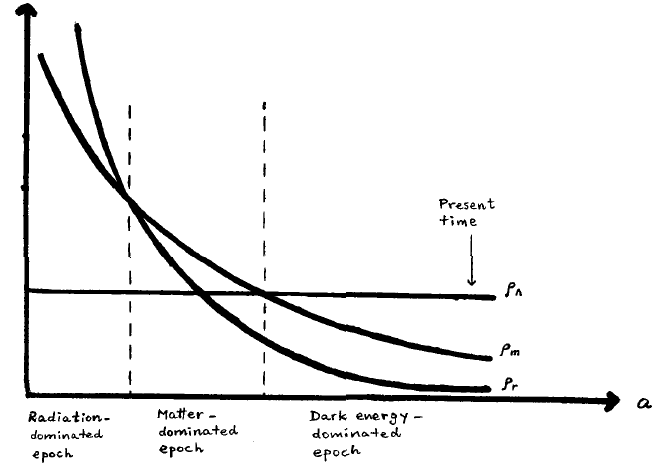
\includegraphics[scale=0.6]{Draw/lec6_2.png}
\end{center}
\caption{Evolution of the energy components of the universe}
\label{fig:lec6_2}
\end{figure}

\subsection{The universe with no dark energy}

We are now ready to study how the scale factor $a(t)$ changes in time. In this section we will consider a hypothetical universe with no dark energy, so we will set $\rho_{\Lambda}=0$. The Friedmann equation (\ref{eq:friedmann_eq}) then takes the form
\begin{equation} \label{eq:friedmann_eq1}
\left(\frac{\dot{a}}{a}\right)^2=\frac{8\pi G}{3c^2}\left( \frac{\rho_m(t_0)}{a^3}+\frac{\rho_r(t_0)}{a^4} \right)-\frac{kc^2}{R^2a^2}.
\end{equation}
Finding the exact solution of this equation is not easy, but we can get a qualitative understanding of how $a(t)$ evolves just by looking at the right-hand side of (\ref{eq:friedmann_eq1}). Consider first the cases where $k=0$ or $k=-1$. It is clear that, in these two cases, the right-hand side of the Friedmann equation is always positive, which implies that $\dot{a}(t)>0$ for all $t$. What this says is that the scale factor always increases in time, and so the universe will expand forever in the cases where $k=0$ or $k=-1$. This scenario is known as the Big Freeze (or the Big Chill), because the temperature of the universe will keep decreasing as the expansion continues.

Consider next the case $k=+1$. The curvature term is now negative (because of the negative sign), and so as $a$ increases this term will eventually become as large as the first term on the right-hand side of eq.\ (\ref{eq:friedmann_eq1}). At this time, then, we will have that $\dot{a}(t)=0$, which means that the expansion of the universe will stop. The universe will then begin to {\it contract}, and it will eventually recollapse in what is known as the Big Crunch (see fig.\ \ref{fig:lec6_3}).
\begin{figure}[ht]
\begin{center}
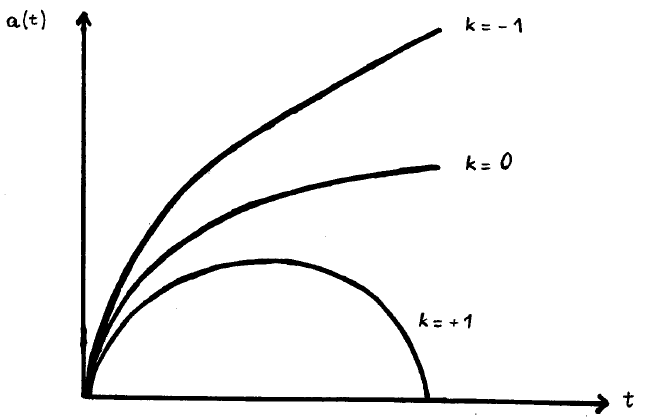
\includegraphics[scale=0.5]{Draw/lec6_3.png}
\end{center}
\caption{The universe with no dark energy}
\label{fig:lec6_3}
\end{figure}

\par\vspace{\baselineskip}

{\bf Exercise.} In the case $k=+1$, show that the value of $a$ at which $\dot{a}=0$ is given by
\begin{equation}
a=\frac{4\pi G}{3c^4}\frac{R^2}{k}\rho_m(t_0)\left[1+\sqrt{1+\frac{3c^4}{2\pi G}\frac{k}{R^2}\frac{\rho_r(t_0)}{\rho_m(t_0)^2}}\right].
\end{equation}

\par\vspace{\baselineskip}

We can then distinguish three types of universes depending on the spatial geometry and the evolution of the scale factor:
\begin{itemize}
\item Flat universe ($k=0$): The universe has zero spatial curvature, it is infinite in size, and it expands forever.
\item Open universe ($k=-1$): The universe has negative spatial curvature, it is infinite in size, and it expands forever.
\item Closed universe ($k=+1$): The universe has positive spatial curvature, it is finite in size, and it eventually recollapses.
\end{itemize}
Notice that the fact that the closed universe is finite in size does not mean that it has a boundary. If we start traveling in some direction we are not eventually going to find a wall at which the universe ends, but instead we are going to come back to the place where we started. This may seem odd for our ``Euclidean'' minds, which are not used to think in 3-dimensional curved spaces. However, the 2-dimensional analogy of the sphere is useful to understand this point. The space defined by the surface of a sphere is also a finite space with no boundaries; here if you walk in some direction (along the equator, for instance) you will eventually come back to the starting point. The same happens in the case of a closed universe, which has the spatial geometry of a 3-dimensional sphere.

\subsection{The universe with dark energy}

As we will see in a later lecture, today we have compelling evidence that there is dark energy in the universe. In fact, we will see below that dark energy is the dominant source of energy at the present time. If $\rho_{\Lambda}>0$ the Friedmann equation reads
\begin{equation} \label{eq:friedmann_eq2}
\left(\frac{\dot{a}}{a}\right)^2=\frac{8\pi G}{3c^2}\left( \frac{\rho_m(t_0)}{a^3}+\frac{\rho_r(t_0)}{a^4}+\rho_{\Lambda} \right)-\frac{kc^2}{R^2a^2}.
\end{equation}
There is no simple analytical solution to this equation. However, notice that the right-hand side of (\ref{eq:friedmann_eq2}) is always positive at late times, regardless of the value of $k$, thanks to the presence of the constant term proportional to $\rho_{\Lambda}$. This means that $\dot{a}(t)>0$ for large $t$, and so the scale factor will increase in time without bound. Thus, at late times we will have that $a\gg1$, implying that all the terms on the right-hand side of (\ref{eq:friedmann_eq2}) will be small, with the exception of the constant dark energy term, which is independent of $a$. In other words, the dark energy density will always dominate over the other energy sources (and over the curvature term) at sufficiently late times. Then, at late times, we can write the Friedmann equation in the approximate form
\begin{equation}
\left(\frac{\dot{a}}{a}\right)^2=\frac{8\pi G}{3c^2}\rho_{\Lambda},
\end{equation}
\begin{equation}
\Rightarrow~~~~\dot{a}=\sqrt{\frac{8\pi G}{3c^2}\rho_{\Lambda}}~a.
\end{equation}
If we take the time derivative of the last equation we obtain
\begin{equation}
\begin{split}
\ddot{a}&=\sqrt{\frac{8\pi G}{3c^2}\rho_{\Lambda}}~\dot{a}\\
&=\left(\frac{8\pi G}{3c^2}\rho_{\Lambda}\right) a,
\end{split}
\end{equation}
where $\ddot{a}(t)$ denotes the second time derivative of $a(t)$. The important conclusion is that $\ddot{a}(t)>0$ at late times. What this says is that the rate of expansion, $\dot{a}$, is itself increasing in time. In other words, the expansion of the universe is accelerating! The observation of this cosmic acceleration is one the most important discoveries of the past two decades, as it provided compelling evidence for the existence of dark energy (although other explanations exist, as we will see later). The qualitative evolution of the scale factor, in the presence of dark energy, is shown in fig.\ \ref{fig:lec6_4}. Notice that when $\rho_{\Lambda}>0$ the universe will expand forever in the future, regardless of the value of $k$, and regardless of whether the universe is finite or infinite in size.
\begin{figure}[ht]
\begin{center}
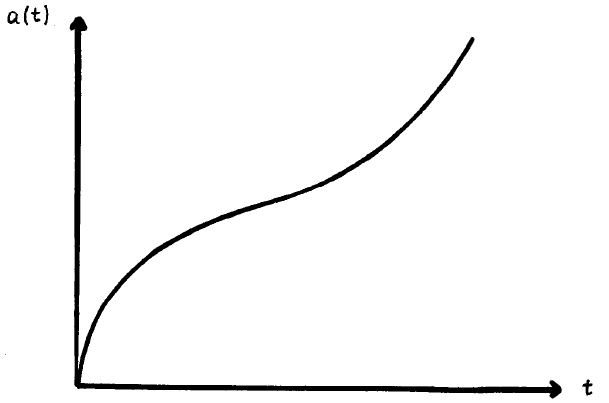
\includegraphics[scale=0.5]{Draw/lec6_4.png}
\end{center}
\caption{The universe with dark energy}
\label{fig:lec6_4}
\end{figure}

\subsection{Density parameters}

In this subsection we introduce the density parameters, which are useful tools used by cosmologists. First, recall the definition of the Hubble parameter,
\begin{equation}
H(t)\equiv \frac{\dot{a}(t)}{a(t)}.
\end{equation}
Recall also that the Hubble constant is simply the present value of the Hubble parameter: $H_0\equiv H(t_0)$, where $t_0$ denotes the present time. We can then write the Friedmann equation (\ref{eq:friedmann_eq}) in terms of $H(t)$ as follows:
\begin{equation}
H(t)^2= \frac{8\pi G}{3c^2}\rho(t)-\frac{kc^2}{R^2a(t)^2}.
\end{equation}
Dividing this equation by $H(t)^2$ we get
\begin{equation} \label{eq:friedmann_eq3}
1= \frac{8\pi G}{3c^2H(t)^2}\rho(t)-\frac{kc^2}{R^2H(t)^2a(t)^2}.
\end{equation}
Next define the {\it critical density} as
\begin{equation} \label{eq:crit_dens}
\rho_c(t)\equiv \frac{3c^2H(t)^2}{8\pi G}.
\end{equation}
The present value of $\rho_c$ (divided by $c^2$ to get a mass density) is given by
\begin{equation}
\begin{split}
\frac{\rho_c(t_0)}{c^2}&=\frac{3H_0^2}{8\pi G}\\
&\approx 10^{-26}~\mathrm{kg~m^{-3}}\approx 10^{11}~M_{\odot}~\mathrm{Mpc^{-3}},
\end{split}
\end{equation}
where $M_{\odot}$ denotes the solar mass. Using definition (\ref{eq:crit_dens}) in eq.\ (\ref{eq:friedmann_eq3}) we find
\begin{equation} \label{eq:friedmann_eq4}
1=\frac{\rho(t)}{\rho_c(t)}-\frac{kc^2}{R^2H(t)^2a(t)^2}.
\end{equation}
Finally, define the {\it density parameter} $\Omega(t)$ as
\begin{equation}
\Omega(t)\equiv \frac{\rho(t)}{\rho_c(t)}.
\end{equation}
Eq.\ (\ref{eq:friedmann_eq4}) can then be rewritten as
\begin{equation}
\Omega(t)-1=\frac{kc^2}{R^2H(t)^2a(t)^2}.
\end{equation}
Evaluating this last equation at $t=t_0$ (the present time), we find\footnote{Recall that $a(t_0)=1$ by definition.}
\begin{equation}
\Omega(t_0)-1=\frac{kc^2}{R^2H_0^2},
\end{equation}
\begin{equation} \label{eq:curvature_dens_param}
\Rightarrow~~~~\frac{k}{R^2}=\frac{H_0^2}{c^2}\left(\Omega(t_0)-1\right).
\end{equation}
Eq.\ (\ref{eq:curvature_dens_param}) is very useful, because it allows us to find the values of $k$ and $R$ if we know the values of $H_0$ and $\Omega(t_0)$, which can be directly measured. However, observations tell us that $\Omega(t_0)\approx1$, which implies that the right-hand side of eq.\ (\ref{eq:curvature_dens_param}) is approximately (if not exactly) zero. Therefore the left-hand side must also be zero or very close to zero. This means that either $k=0$ (and the universe is flat), or $k\neq0$ but $R$ is very large. Unfortunately, then, we cannot tell experimentally whether the universe is finite or infinite in size; however, if it is finite (so that $k=1$), then it must be much larger than the observable universe (whose size is of the order of $c/H_0$). The reason why $\Omega(t_0)$ is so close to unity is an important puzzle in cosmology; the theory of inflation (which we will study in a later lecture) is widely believed to provide the correct solution to this question.

Let us define next the density parameters for the matter, the radiation, and the dark energy, as follows:
\begin{equation}
\begin{split}
\Omega_m(t)&\equiv \frac{\rho_m(t)}{\rho_c(t)},\\
\Omega_r(t)&\equiv \frac{\rho_r(t)}{\rho_c(t)},\\
\Omega_{\Lambda}(t)&\equiv \frac{\rho_{\Lambda}}{\rho_c(t)}.\\
\end{split}
\end{equation}
The total density parameter $\Omega(t)$ can then be written as
\begin{equation}
\begin{split}
\Omega(t)&= \frac{\rho(t)}{\rho_c(t)}\\
&=\frac{\rho_m(t)}{\rho_c(t)}+\frac{\rho_r(t)}{\rho_c(t)}+\frac{\rho_{\Lambda}(t)}{\rho_c(t)},
\end{split}
\end{equation}
\begin{equation}
\Rightarrow~~~~\Omega(t)=\Omega_m(t)+\Omega_r(t)+\Omega_{\Lambda}(t).
\end{equation}
Let us look at the different energy components of the universe more closely. The matter in the universe includes the following:
\begin{itemize}
\item Baryonic matter (protons, neutrons, electrons)
\item Dark matter
\end{itemize}
We can accordingly write the matter density parameter as the sum of the baryonic density parameter, $\Omega_b(t)$, and the dark matter density parameter, $\Omega_{DM}(t)$. Thus,
\begin{equation}
\Omega_m(t)=\Omega_b(t)+\Omega_{DM}(t).
\end{equation}
Do not confuse dark matter with dark energy. Whereas dark energy is a form of energy whose nature is unknown, dark matter is really just another form of matter, meaning that it is composed of particles (there are however alternative theories, as we will see later in the course). The problem is that physicists do not know what kind of particle it is. We know that dark matter exists because of the gravitational force it exerts on stars and galaxies, but it is not known whether it interacts via any of the other forces. In particular, dark matter does not interact via the electromagnetic force, meaning that it cannot emit or absorb light (hence the name ``dark'').

The radiation in the universe includes all relativistic particle species, which at the present time are given by the following:
\begin{itemize}
\item Photons
\item Neutrinos
\end{itemize}
Photons are massless particles, and so they move at the speed of light and are therefore always relativistic. Neutrinos, on the other hand, are particles with very small, but nonzero masses. In the context of cosmology, the question of whether a massive particle is relativistic or not depends on its temperature. If the temperature is large, such that the thermal energy of a given particle (which is a measure of the mean kinetic energy) is larger than the rest energy, then the particle will be relativistic. If, on the other hand, the rest energy is much larger than the thermal energy (as occurs to baryons today), then the particle will be nonrelativistic. Since we do not know the precise values of the neutrino masses (and therefore we do not know the rest energy of a neutrino), we cannot actually be sure that neutrinos are relativistic today. However, we do know that neutrinos have been relativistic for most of the history of the universe, so that their relative importance in cosmology is similar to that of 
photons. This is why we will usually study neutrinos as being part of the radiation component of the energy in the universe.

With this in mind, we can write the radiation density parameter as the sum of the photon density parameter, $\Omega_{\gamma}(t)$, and the neutrino density parameter, $\Omega_{\nu}(t)$. Thus,
\begin{equation}
\Omega_r(t)=\Omega_{\gamma}(t)+\Omega_{\nu}(t).
\end{equation}

Finally, we can write the present density parameter $\Omega(t_0)$ in terms of all the different energy components present in the universe:
\begin{equation}
\Omega(t_0)=\Omega_b(t_0)+\Omega_{DM}(t_0)+\Omega_{\gamma}(t_0)+\Omega_{\nu}(t_0)+\Omega_{\Lambda}(t_0).
\end{equation}
Experimentally, these are given by
\begin{equation}
\begin{split}
\Omega_{\gamma}(t_0)&\approx 5\times10^{-5},\\
\Omega_{\nu}(t_0)&\approx 3\times10^{-5},\\
\Omega_{b}(t_0)&\approx 0.04,\\
\Omega_{DM}(t_0)&\approx 0.26,\\
\Omega_{\Lambda}(t_0)&\approx 0.70.
\end{split}
\end{equation}
As we mentioned above, the energy density today is dominated by the dark energy, which is about $70\%$ of the total energy. It is followed by the matter energy density, which today is about $30\%$ of the total energy. Finally, the radiation presently contributes only a small fraction to the energy density in the universe (see fig.\ \ref{fig:lec6_2}). Notice the (embarrasing) fact that $96\%$ of the energy density in the universe is in the form of dark matter and dark energy, whose exact nature is unknown.

\section{Aside on particle physics}

In this section we will make a quick introduction to particle physics. This will be useful for our study of the thermal history of the universe during this and next lectures.

There are four types of interactions (or forces) in nature: electromagnetic, weak, strong, and gravitational. Each interaction is mediated by one or more particles called {\it bosons}.\footnote{More precisely, the particles that mediate the interactions are called gauge bosons. A different type of boson is the Higgs, whose role is to give mass to all the other particles.} These are shown in the following table:
\begin{table}[ht]
\begin{center}
\begin{tabular}{p{4cm} l l} \hline\hline
Interaction & Boson  \\ \hline
Electromagnetic & Photon \\
Weak & $W^{+}$, $W^{-}$, $Z^0$ \\
Strong & Gluon \\
Gravitational & Graviton \\ \hline\hline
\end{tabular}
\end{center}
\end{table}

The particles that form matter (including antimatter and unstable matter) are called {\it fermions}. Fermions are divided into {\it leptons} and {\it quarks}. Leptons are further divided into charged leptons and neutrinos. This classification is summarized in the following diagram:
\begin{equation*}
\mbox{Fermions }\begin{cases} \mbox{$~~$Leptons } \begin{cases} \mbox{$~~$Charged leptons}\\ ~\\ \mbox{$~~$Neutrinos}\end{cases}\\ 
~\\
\mbox{$~~$Quarks} \end{cases}
\end{equation*}
Each fermion has a corresponding antiparticle, which has the same mass but opposite quantum numbers. For example, if a particle has negative electric charge the antiparticle has a positive electric charge of the same magnitude. The different fermions presently known are described in the following:
\begin{itemize}
\item Charged leptons: electron ($e^{-}$), muon ($\mu^{-}$), tau ($\tau^{-}$) (antiparticles: $e^{+}$, $\mu^{+}$, $\tau^{+}$). They interact via the electromagnetic, the weak, and the gravitational forces.
\item Neutrinos: electron neutrino ($\nu_e$), muon neutrino ($\nu_{\mu}$), tau neutrino ($\nu_{\tau}$) (antiparticles: $\bar{\nu}_e$, $\bar{\nu}_{\mu}$, $\bar{\nu}_{\tau}$). They interact via the weak and the gravitational forces.
\item Quarks: up ($u$), down ($d$), strange ($s$), charm ($c$), bottom ($b$), top ($t$) (antiparticles: $\bar{u}$, $\bar{d}$, $\bar{s}$, $\bar{c}$, $\bar{b}$, $\bar{t}$). They interact via the electromagnetic, the weak, the strong, and the gravitational forces.
\end{itemize}
An important property of quarks is called {\it quark confinement}: at temperatures below $T\sim 2\times10^{12}$ K, quarks cannot be found as free particles, but are confined within composite particles known as {\it hadrons}.\footnote{Compare the quark confinement temperature with the temperature at the core of the Sun: $1.6\times10^7$ K.} There are two types of hadrons: {\it baryons} (particles formed by 3 quarks), and {\it mesons} (particles formed by 2 quarks). Examples of baryons include the familiar proton and neutron.\footnote{An important note on terminology: In astrophysics and cosmology people often refer to protons, neutrons and electrons as ``baryons,'' although electrons are not really baryons in the classification of particle physics.} Examples of mesons include the pion and the kaon.
\begin{equation*}
\mbox{Hadrons }\begin{cases} \mbox{$~~$Baryons} \\ 
~\\
\mbox{$~~$Mesons} \end{cases}
\end{equation*}

The picture we have just decribed is known as the Standard Model of particle physics, and it is one of the most successful theories in the history of physics (fig.\ \ref{fig:lec6_5}).\footnote{Actually, the graviton has not been detected yet, and it is not part of the Standard Model} We know, however, that this picture has to be incomplete: it does not include dark matter. Dark matter interacts only via the gravitational force, and perhaps via the weak force. The only candidate with these properties, within the Standard Model, is the neutrino. However, we will see later that, because of their very small mass, neutrinos cannot be the dark matter, which means that we have to look at other theories that include new (and so far unobserved) particles for possible dark matter candidates.
\begin{figure}[ht]
\begin{center}
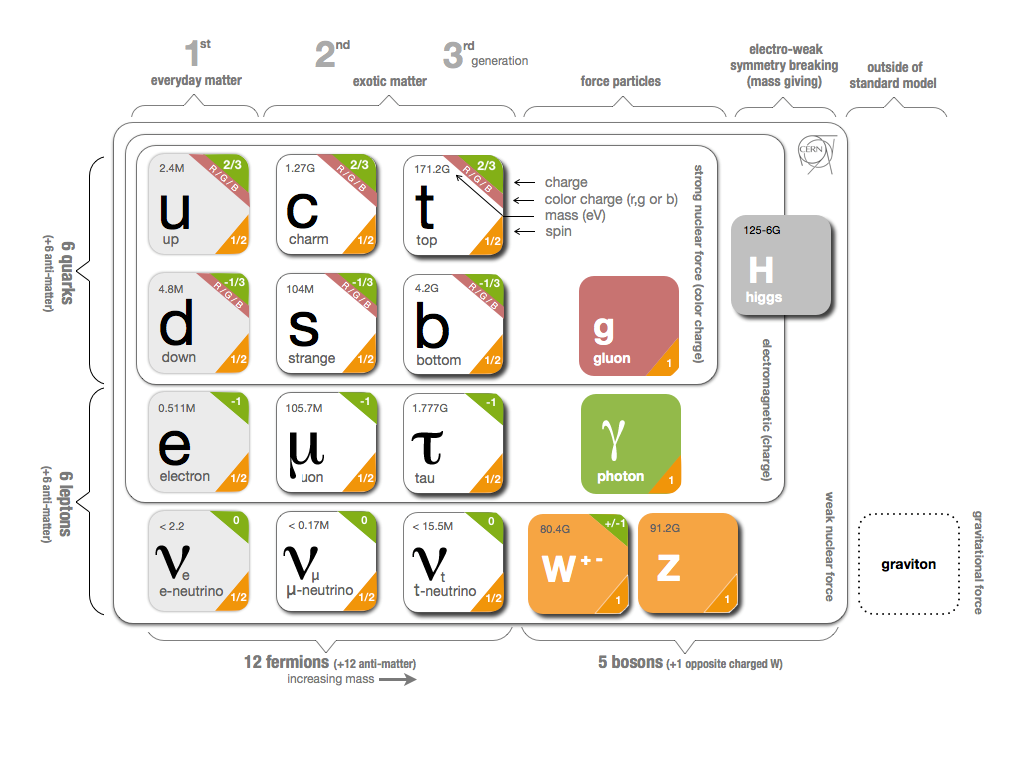
\includegraphics[scale=0.35]{Draw/lec6_5.png}
\end{center}
\caption{The particles of the Standard Model (Source: \url{http://www.isgtw.org})}
\label{fig:lec6_5}
\end{figure}

\section{The thermal history of the universe}
\label{chp7}

The early universe can be thought of as a soup (more technically a plasma) of {\it primordial particles} (particles created during the very first instants after the Big Bang) continuously interacting with each other in a state of thermal equilibrium. A fluid or plasma in thermal equilibrium can be described by its temperature $T$, which is a measure of the average kinetic energy of the particles. Immediately after the Big Bang the temperature of the cosmic plasma is infinitely high, and then begins to continuously decrease as the universe expands. In fact, we will see in a later lecture that $T\propto 1/a$ during most of the history of the universe.

The strength at which particles interact depends on their kinetic energy, and therefore on the temperature of the plasma. At very high temperatures, all interactions are effective and all particles are maintained in thermal equilibrium with the plasma. As the temperature decreases, however, some interactions become inefficient and some particle species may fall out of equilibrium with the plasma, in a process known as {\it decoupling}, and subsequently travel freely through the universe, without further scatterings with the other particles in the plasma. This is what happened to neutrinos when the universe was only $0.2$ seconds old, and later to photons when the universe was about $380,000$ years old.\footnote{There is also an earlier stage at which dark matter particles decoupled from the cosmic plasma. The details of this stage are largely unknown, and so we will omit it in the following outline.}

In what follows we will make a quick outline of the main phases of the thermal history of the universe, with the corresponding times and temperatures. In the following lectures we will cover some these phases in much more detail.

\begin{itemize}

\item $t\sim 10^{-5}$ s, $T\sim 2\times10^{12}$ K: Quark confinement.

By this time all the muons and tau leptons, as well as all the quarks heavier than the $u$ and $d$, have decayed. The cosmic plasma now contains electrons, neutrinos, $u$ quarks, $d$ quarks, and photons. After this time quarks become confined and form the first protons and neutrons.

\item $t\sim 0.2$ s, $T\sim 10^{10}$ K: Neutrino decoupling.

Neutrinos interact with the other particles in the plasma only via the weak force (and also via the gravitational force, but this is completely negligible). This is what keeps the neutrinos in thermal equilibrium with the plasma. However, when the temperature drops below $T\sim 10^{10}$ K, the weak interaction becomes inefficient. Neutrinos then decouple from the plasma and begin to propagate freely without further interactions.

\item $t\sim 200$ s, $T\sim 5\times10^8$ K: Nucleosynthesis.

At temperatures above $T\sim 5\times10^8$ K protons and neutrons are free; they cannot bind together to form heavier atomic nuclei (such as helium), since the photons in the plasma immediately destroy them. This effect is known as {\it nuclear photodissociation}. When the temperature drops below $T\sim 5\times10^8$ K the photons are not energetic enough to destroy the nuclei effectively, and protons and neutrons can now combine to form the first atomic nuclei: deuterium ($^2$H), tritium ($^3$H), helium-3 ($^3$He), helium-4 ($^4$He), and lithium ($^7$Li). This process is known as {\it nucleosynthesis}.

\item $t\sim 10^{13}$ s, $T\sim 4\times10^3$ K: Recombination.

By this time the cosmic plasma contains electrons, photons, and atomic nuclei. At temperatures above $T\sim 4\times10^3$ K there are no neutral atoms; as soon as an electron is captured by a nucleus to form a neutral atom, it is immediately kicked out by a photon in a process known as {\it photoionization}. When the temperature drops below $T\sim 4\times10^3$ K the photons in the plasma are not energetic enough to ionize the atoms effectively. As a result, electrons quickly become captured by atomic nuclei and the universe becomes neutral: it now contains only atoms, photons, neutrinos, and dark matter. This process is known as {\it recombination}. Since photons can only interact with electrically charged particles, after recombination the primordial photons decouple and begin to propagate without further interactions. These are the photons that we can observe today in the cosmic microwave background (CMB).

\item $t\sim 10^{16}-10^{17}$ s: Structure formation.

After recombination the cosmic plasma disappears. The remaining neutral atoms (as well as the dark matter) begin to clump together as a result of gravity. Eventually the lumps of atoms grow larger and larger until they form the first stars and galaxies. This is the process of {\it structure formation}, which includes several stages whose exact details are not yet fully understood.

\end{itemize}


\chapter{The thermal history of the universe}

\section{Introduction}
The goal of this chapter is that of going deeper in understanding something mentioned in the previous one: the thermal history of the Universe. In particular we want to understand how our universe tranformed from a hot, uniform soup of particles originated at the time of Big Bang, into the variety of atoms, molecules, planets, stars and galaxies that we see today. What we will cover in this section is the history of the universe up to when the first atoms, hydrogen, appeared; this epoch is really important in the study of cosmology because this is the time at which the Cosmic Microwave Background, which is one of the most solid observable evidences we have, originated. We shall see that the important epochs in the uiniverse history are characterized by the presence of different kind of particles and are characterized by different temperature scales $T$. In the first part of the lecture we will try to understand what is the meaning of these temperatures, i.e. how can we define the concept of temperature when 
we talk about the universe; in the following we will introduce some useful concepts to quantify the interactions between different kind of particles, and how these interactions depend strongly on the temperature scale. Finally, equipped with these tools, we will be able to study the most relevant steps in the history of the universe: the origin of nuclei, atoms and the cosmic microwave background. 

\section{The meaning of temperature}
You may recall that in some of the previous lectures we already encountered the concept of temperature, for example we saw several times that the measured temperature of the CMB (whatever this means) is $T=2.78$\,K: what is the precise meaning of that? We know that the CMB is made of photons, so what does it mean to associate a temperature to photons? We know from thermodynamics that, for a regular gas of particles (helium, hydrogen, air,...) the temperature is a measure of the average kinetic energy per particle $\langle U_{kin}\rangle$ according to the relation
\begin{equation}
\langle U_{kin}\rangle =\frac{3}{2}k_BT
\end{equation}
Where $k_B=1.38\cdot 10^{-23}$\,J/K is called Boltzmann constant; how can we extend this concept to photons? Photons are the particles which make up light and, for an e.m. (light) wave of frequency $\nu$, the photons which compose it carry a kinetic energy $U_{kin}=h\nu$ each ($h=6.63\cdot 10^{-34}$\,Js is called Planck constant). We are tempted to define temperature for photons in the same way as we did for the regular gas, and in some sense we can. We have to answer the question in an ensembleof photons (think about a oven for baking bread for example) at temperature $T$, what is their average kinetic energy? Statistical mechanics helps us in this one, stating that the probability of finding a particle with an energy $E$ in a system of temperature $T$ \textit{at thermal equilibrium} is proportional to $e^{-E/k_BT}$. This tells us that the prooability of finding $n$ photons of frequency $\nu$ in our oven is proportional to $e^{-nh\nu/k_BT}$. This allows us to compute the average number density and total 
energy density of all the photons of frequency $\nu$ as 
\begin{equation}
\langle n_\nu\rangle=\frac{1}{V}\frac{\sum_{n=0}^{\infty}ne^{-nh\nu/k_BT}}{\sum_{n=0}^{\infty}e^{-nh\nu/k_BT}}
\end{equation}
And the total energy density of these photons will be $u_\nu=h\nu \langle n_\nu\rangle$; performing the sum we get to an expression for the energy density $u_\nu$ of the photons of frequency $\nu$ in our oven as 
\begin{equation}
\label{planck}
u_\nu=\frac{8\pi h\nu^3}{c^3}\frac{1}{e^{h\nu/k_BT}-1}
\end{equation}
From this quantity we can derive the so called \textit{spectral radiance} $B_\nu(T)=\frac{c}{4\pi}u_\nu(T)$ which is the amount of energy of modes of frequency $\nu$, that crosses a unit area travelling in a certain direction, per unit time (it is measured in J s$^{-1}$ Area$^{-1}$ Hz$^{-1}$ steradian$^{-1}$); this is the quantity that is actually measured in experiments (like telesciopes, which measure the amount of energy received in a certain frequency band), when we look at our oven (or at the universe, which you may think of as a big, expanding oven) from inside. If we plot $B_\nu$ versus $\nu$ for different temperatures we obtain something like Figure \ref{blackbody1}.
\begin{figure}
\begin{center}
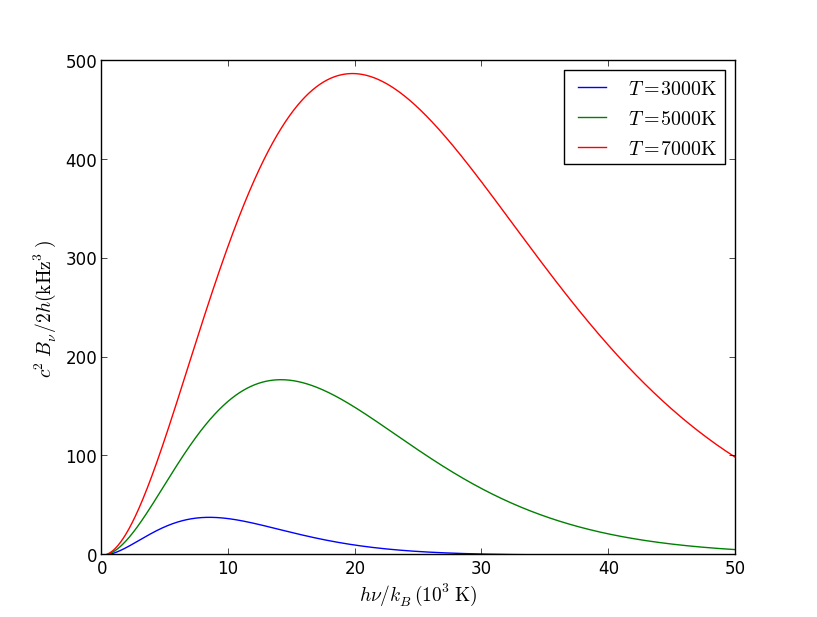
\includegraphics[scale=0.7]{Draw/blackbody.png}
\label{}
\end{center}
\caption{A plot of the spectral radiance $B_\nu$ versus $\nu$ for different temperatures $T$; you can notice that different curves peak at different frequencies. This fact is expressed by Wien's law that states $\frac{cT}{\nu_{peak}}=2.89\cdot10^{-3}\,$m$\cdot$K}
\label{blackbody1}
\end{figure}
You can see that, since observations today are able to probe a wide range of frequencies, looking at the shape of the curve and at the position of its peak, we are able to measure the temperature of our system (just choosing the best $T$ that fits our data); a system that has a spectral radiance which has a frequency distribution as in Figure \ref{blackbody1} is called a \textit{blackbody}. In nature there are a lot of systems that behave like blackbodies, in a very large range of temperatures, as outlined in Table \ref{blackbodies}
\begin{table}[htdp]
\begin{center}
\begin{tabular}{|c|c|} \hline
\textbf{System} & \textbf{Blackbody temperatute} $T$ \\ \hline
The sun photosphere & 6000K \\ \hline
Your kitchen's oven & 450K \\ \hline
Earth's atmosphere & 300K \\ \hline
The Cosmic Microwave Background & 2.78K \\ \hline
Hawking radiation from black holes & Few fractions of K (too small to be detected) \\ \hline
\end{tabular}
\end{center}
\caption{Some physical systems that behave like blackbodies}
\label{blackbodies}
\end{table}
Now imagine that our universe (or big oven) expands: we already know that photons are redshifted, and this causes their energy to shift to low values. What effects does this have on the spectral radiance $B_\nu$? Clearly we have a redistribution of photon energies over all the spectral band, but remember that, when the universe's size grows by a factor $a$, \textit{all} the photons with frequency $\nu$ become photons with frequency $\nu'=\nu/a$. This means that, if we assume that no photons are created or destroyed
\begin{equation}
n_\nu d\nu=n_{\nu'}d\nu'a^3
\end{equation}
Now, remember from equation (\ref{planck}) that the photon number density is proportional to $n_\nu \propto \nu^2$ and that $\frac{d\nu}{d\nu'}=a$, and this means that $\frac{n_\nu}{\nu^2}=\frac{n_\nu'}{\nu'^2}$, which tells us that the spectral radiance of the expanding system \textit{has to maintain the shape of a blackbody} but in general with a new temperature $T'$ which can be derived observing that
\begin{equation}
\frac{1}{e^{h\nu/K_BT}-1}=\frac{1}{e^{h\nu'/k_B T'}}
\end{equation}
Which tells us immediately that $T'=T/a$; in this sense the universe \textit{cools down} as it expands; what does all this have to do with our study of cosmology? In 1990 the COBE satellite measured the spectral radiance of the Cosmic Microwave Backgronud, and their experimental data looked like Figure \ref{cmbspectral}
\begin{figure}
\begin{center}
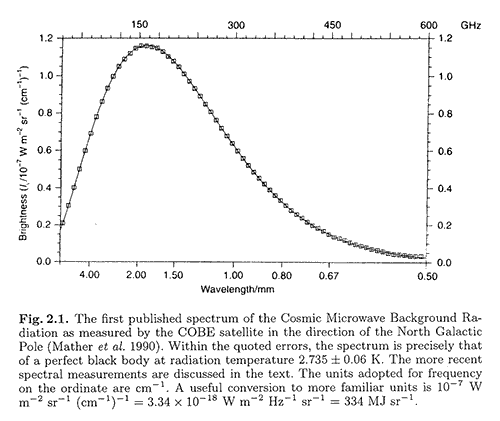
\includegraphics[scale=0.7]{Draw/cmbrad.png}
\label{}
\end{center}
\caption{Spectral radiance of the CMB as measured by the COBE satellite; the curve is consistent with a blackbody shape with a temperature of 2.78K. COBE experiment reference \url{http://lambda.gsfc.nasa.gov/product/cobe/c_images.cfm}}
\label{cmbspectral}
\end{figure}
This tells us two things: our universe today is \textit{very cold}, but when this CMB originated in the past, it could have been much hotter (we will see that it was at least 1000 times hotter. This radiation exibits a blackbody shape: it means that, when it originated in the past, the universe was in \textit{thermal equilibrium}; we will see that this is not true anymore today because the universe is almost neutral and hence ordinary matter has only very weak interactions with the photons. The picture in the subsequent paragraphs will be the following: the universe is composed by a lot of particles of different kind (photons, electrons, neutrinos, nuclei,...) that interact with each other with the three fundamental forces in the standard model (electromagnetic, strong force, weak force). Some of these interactions might be very efficient, some others less efficient, depending on the temperature of the system (we will outiline the important epochs in the \textit{thermal history of the universe} i.e. we will 
identify the temperatures at which each different interacton undergoes a drastic change in its efficiency). In principle each kind of particle can have its own temperature $T_i$, but all these temperatures are the same if all the species are in thermal equilibrium; for this reason, in the following we will refer to the \textit{temperature of the photons} as \textit{the temperature of the universe}, because photons are the particles which interact the most efficiently with matter, and are the last species to drop off thermal equilibrium. Before going into the actual thermal history of the universe, we need to understand better what does it mean that an interaction is \textit{efficient} or not; we will do this in the following paragraph. 

\section{When is an interaction considered efficient?}
\subsection{Particles number density}
\label{densities}
We have already seen in the previous lecture that the particles which compose the universe can be distinguished roughly in two big categories: hot particles that move close to the speed of light (photons and neutrinos) and cold particles which move at speeds much lower than $c$. The laws of thermodynamics tell us that these different kind of particles have very different number densities when they are in thermal equilibrium; in particular we have
\begin{itemize}
\item $n_{hot}(T)\propto T^3$ for hot particles; a particle species is considered hot, or relativistic, when its mass is very low compared to the typical energy scale, or $mc^2\ll k_BT$
\item $n_{cold}(T)\propto T^{3/2}e^{-mc^2/k_BT}$ for cold particles; a particle species is considered cold, or non relativistic when its mass is very big compared to the typical energy scale, or $mc^2\gg k_BT$. Note that for this main reason, and the exponential factor in $n_{cold}$ at equal temperature scales in general $n_{cold}\ll n_{hot}$
\end{itemize} 
\subsection{The strength of interactions}
We know that different kinds of particles can interact with each other according to the standard model, for example electrons interact with photons or neutrinos, protons interact with neutrons and they bind together to form nuclei, etc... How do we know how \textit{strong} each one of these interaction is? In particle physics the strength of an interaction process is quantified by a number, with measure units of an area, that is called \textit{cross section} and is usually denoted with the letter $\sigma$. To understand the precise meaning of this number, consider the following example in Figure \ref{crossec}
\begin{figure}
\begin{center}
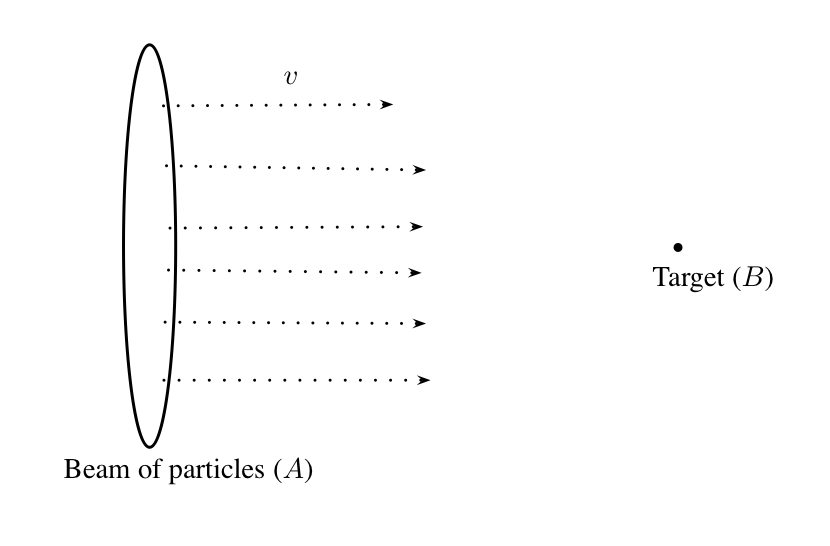
\includegraphics[scale=0.7]{Draw/cross_section.png}
\label{}
\end{center}
\caption{Illustrative example of an interaction of particles of species $A$ with particles of species $B$}
\label{crossec}
\end{figure}
Suppose we have a beam of particles of species $A$ that travel at velocity $v$ and are directed to a fixed target of particles of species $B$; a good way to characterize the strength of the interaction between $A$ and $B$ is to look at how many interactions will take place. If there are few the interaction is small, if there are many, the interaction is big; that's where the concept of cross section comes in hand. The cross section $\sigma_{AB}$ of an interaction process between $A$ and $B$ is defined as the \textit{effective area} that target $B$ offers to projectile $A$ for being hit. More quantitatively, if we call $\Sigma$ the numer of particles per unit area in the beam and $N_{int}$ the total number of interactions that take place, we should have
\begin{equation}
N_{int}=\Sigma \sigma_{AB}
\end{equation}
An important feature of this cross section is that it does not depend on the intensity of the beam or on the number of targets, but \textit{only} on the details of the interaction between $A$ and $B$ (it can depend on the energy scale of the collision though). To go onto more practical grounds, consider the following examples
\begin{itemize}
\item When we consider the collision of two solid balls of radius $R$ obviously the cross section associated with this process is $\sigma=\pi R^2$
\item Condider a photon ($\gamma$) - electron ($e^-$) at low energy (the so called \textit{Thomson scattering}): classical electrodynamics tells us that the cross section for this process is $\sigma_{th}=\frac{8\pi}{3}\left(\frac{e^2}{m_ec^2}\right)^2\approx0.66\cdot 10^{-28}\mathrm{m}^2$. The quantity $r_e=\frac{e^2}{m_ec^2}\sim 10^{-14}$m has dimensions of length and can be interpreted as the effective size of an electron. Note that this effective size does not have an absolute meaning (you won't be able to measure it with a ruler), but has only meaning in quantifying the interaction between electrons and photons
\item A photon - electron interaction at high energy (\textit{Compton scattering}) $\epsilon \gg m_ec^2$; the cross section for this process computed in full quantum electrodynamics is 
\begin{equation}
\sigma_{comp}\approx \pi r_e^2\left(\frac{\ln{\frac{2\epsilon}{m_ec^2}}}{\frac{\epsilon}{m_ec^2}}\right)
\end{equation} 
\item A neutrino ($\nu$) - electron interaction in neutrino energy range $E_\nu\approx 1$MeV has a cross section 
\begin{equation}
\label{neutel}
\sigma_{e\nu}\approx 10^{-48}\mathrm{m}^2\left(\frac{E_\nu}{1\mathrm{MeV}}\right)
\end{equation}
Note that, since this is a weak nuclear interaction process, its cross section is much smaller than a typical electromagnetic cross section $\sigma_{th}$
\item A typical neutron ($n$) - proton ($p$) nuclear collision has a cross section of $\sigma_{np}\approx 10^{-28}$m$^2$ 
\end{itemize} 
\subsection{Efficiency of reactions}
Now that we know how to quantify the \textit{strength} of particle interactions, we have to understand when a particular reaction is considered efficient in cosmological contexts: the fact that an interaction is strong (big $\sigma$), it doesn't mean that the same interaction is efficient. For example if the particles' densities are low, despite of the big cross section, there will be very few interaction events. How do we combine the density and cross section informations to get a good distinguishing criterion? Consider again Figure \ref{crossec}: suppose the impacting beam is composed by particles that travel at velocity $v$ and have a number density $n$; let be $\sigma$ the cross section of this particular interaction. You can convince yourselves that the quantity
\begin{equation}
\tau_{int}=\frac{1}{n\sigma v}
\end{equation} 
has the dimensions of time and represent the average time that elapses by two distinct interaction events; this average time depends jointly on the strength of the interaction and the reactants abundances. Now, remember that both $n,\sigma$ and $v$ depend on the temperature of the system (the equilibrium number densities and average velocities depend on $T$, but the temperature sets also a typical energy scale $E\sim k_BT$, on which the cross section in general depends), so in the end $\tau_{int}$ is a function of $T$. If this timescale is too big and the universe expands too fast bringing all the particles far from each other, clearly the reaction becomes inefficient. The timescale for the universe's expansion is set by the Hubble time, the inverse of the Hubble parameter $t_H=H^{-1}$; since $H$ depends on redshift, and hence on the temperature of the universe (through $T(z)=T_{CMB}/1+z$), we can say that $t_H$ depends on temperature too. We will say then that a reaction is \textit{efficient} if its 
timescale $\tau_{int}$ is much lower than the expansion timescale ($\tau_{int}\ll t_H$). Clearly at the big bang the universe is infinitely hot so all reactions will be efficient and all species will be at thermal equilibrium; for each reaction though, there will be a critical temperature $T_c$ at which $\tau_{int}(T_c)=t_H(T_c)$; below this temperature the reaction will become inefficient. If a particle species has no efficient interactions with the all the other species, it will drop out of thermal equilibrium. Photons are the last one dropping out of equilibrium, and when this happens the CMB is originated: the final goal of this chapter will be understanding when precisely does this happen. 

\section{The important epochs in the universe's life}
In the previous section we saw that a particular interaction process with energy dependent cross section $\sigma(E)$ becomes inefficient when the interaction timescale
\begin{equation}
\tau_{int}(T)=\frac{1}{n(T)\langle\sigma v\rangle_T}
\end{equation}
Becomes bigger than the expansion timescale $t_H=H^{-1}$; roughly speaking, $\tau_{int}$ becomes big when the cross section, the typical velocity, or the number density become small; if a particle species has no effective interaction with the other species, it drops out of thermal equilibrium, or it \textit{decouples}. Based on these considerations we are able to make two important observations:
\begin{itemize}
\item Neutrinos are capable to interact via the weak nuclear force only, their typical interaction cross section is really small, so it is likely that they are the first particle species to drop out of thermal equilibrium; this is precisely what happens
\item Photons have large cross sections (because they interact electromagnetically), the highest speed of all (they travel at the speed of light) and the highest number density (which scales as $T^3$, contrary to other non relativistic species, for which it is depressed by $e^{-mc^2/k_BT}$). For these reasons, it is likely that they are the last species to decouple; when this happens, the CMB is originated. 
\end{itemize}
\subsection{An unknown era}
The universe after the big bang started out really hot, all interaction processes were really efficient and all particles were in thermal equilibrium and could be described in terms of an unique temperature $T$; we don't know more about this period of time, when say $k_BT\gtrsim 1$GeV, because the theoretical tools to understand physics at such high energy scales (namely electroweak theory and quantum chromodynamics) are still under developement. We believe anyway that at a certain point the universe did undergo some kind of phase transition from being a hot soup of quark and gluons (a kind of quark/gluon plasma) to a stage where quarks became confined to form protons and neutrons. This quark/gluon plasma stage constitutes a very active branch of nuclear physics research today. 
\subsection{Neutrinos leave the party}
As said before, neutrinos are the first species to leave thermal equilibrium, because they interact so weakly with the rest of matter; the main process which keeps them coupled is scattering with electrons
\begin{equation}
\nu + e^- \rightarrow \nu + e^-
\end{equation}
With a cross section that scales roughly as (\ref{neutel}); we will be very qualitative in the following, because the computations needed to show the results presented are often lengthy and most of the time require computer algorithms to solve equations numerically. The results of these calculations is that, for this particular process $\tau_{int}\sim t_H$ when $k_BT\sim 1$MeV. At this point neutrinos decouple from the rest of species, and their temperature evolves independently without caring to what happens to the other species, as
\begin{equation}
k_BT_\nu(a)=1\mathrm{MeV}\frac{a(1\mathrm{MeV})}{a}
\end{equation}
The fact that neutrinos decouple means that they originate a sort of background radiation, called \textit{cosmic neutrino background} (or CNB) that free streams towards us; we can estimate the temperature of this radiation knowing the temperature of the CMB. Shortly after  neutrino decoupling, the electron positron annihilation process
\begin{equation}
e^+ + e^- \leftrightarrow \gamma+ \gamma
\end{equation}
becomes really efficient and gets heavily shifted to the right, adding extra photons to the budget; this means that the photon temperature grows (along with the temperature of all the species coupled to them; the neutrino temperature however does not grow, because they are alread decoupled); this heats up the photons by roughly a factor $\sqrt[3]{\frac{11}{4}}$ with respect to neutrinos. We can then estimate that today we expect a temperature
\begin{equation}
T_{CNB}=\sqrt[3]{\frac{4}{11}}T_{CMB}\approx 1.98\,\mathrm{K}
\end{equation}
This corresponds to an energy scale $k_BT_{CNB}\sim 10^{-4}$eV for the neutrinos, which is below any realistic detection threshold for state of art neutrino experiments (which are able to detect neutrinos with energies $\gtrsim 1$keV); unfortunately then there is no realistic hope to detect this cosmic neutrino background in the near future. 
\subsection{The first three minutes: primordial nucleosynthesis}
After the electron neutrino scattering becomes inefficient, neutrinos are still weakly coupled to neutrons and protons via the reactions 
\begin{equation}
\label{proton1}
n+e^+\leftrightarrow p+\bar{\nu}_e
\end{equation}
\begin{equation}
\label{proton2}
n+\nu_e\leftrightarrow p+e^-
\end{equation}
\begin{equation}
n\leftrightarrow p+e^-+\bar{\nu}_e
\end{equation}
The first two reactions become inefficient soon after the neutrino decoupling, precisely after $k_BT\lesssim 0.5$MeV (which corresponds roughly to 1\, second after the Big Bang); the last reaction however may potentially cause a problem. This is not a collision reaction, but rather a decay reaction in which, due to the fact that the neutron is slightly heavier than the proton ($m_n\sim m_p\sim 1$GeV but $m_n-m_p\approx$1.29\,MeV), a neutron can decay and produce lighter particles. The mean lifetime for this decay process is $\tau_n=$15\,minutes. This tells us that, if there is any hope at all to form heavier nuclei (such as deuterium and helium) via strong nuclear interactions, they better form before 15 minutes from the Big Bang, otherwise there may be no neutrons left to bind! Let's see if this is the case. Consider a generic reaction 
\begin{equation}
1+2\leftrightarrow 3+4
\end{equation}
which has associated a cross section $\sigma_{12}$; let's focus on species 1. We want to write down a differential equation for the evolution of its number abundance $n_1$; if there were no interactions, its number density would just decrease due to the fact that the universe is expanding and hence some dilution occurs according to the relation 
\begin{equation}
\label{ateq}
\frac{dn_1}{dt}=-3\frac{\dot{a}}{a}n_1=-3Hn_1
\end{equation}
Due to the interaction with species 2 though,m there might be some injections/subtractions of particles of type 1 in the reaction, quantified by the cross section $\sigma_{12}$ according to 
\begin{equation}
\label{balancenoneq}
\frac{dn_1}{dt}+3Hn_1=n_1^0n_2^0\langle \sigma_{12}v\rangle\left[\frac{n_3n_4}{n_3^0n_4^0}-\frac{n_1n_2}{n_1^0n_2^0}\right]
\end{equation} 
Where $n_i^0$ are the equilibrium number densities as seen in section \ref{densities}; note that the right hand size is close to zero when the reaction is inefficient ($H\gg n\sigma v$) or when the system is at equilibrium $n_i=n_i^0$. In both these cases the system is simple to solve because (\ref{ateq}) has a solution $n_1\propto a^{-3}$; the complicated stage is solving (\ref{balancenoneq}) when the right hand side is non negligible. Usually this can be done only numerically with a computer algorithm, writing down an equation similar to (\ref{balancenoneq}) for each species, when all the cross sections are known. If we apply this method to one of the weak neutron proton reactions (\ref{proton1}) or (\ref{proton2}),along with the information we know about the neutron lifetime, and use a computer to solve for the neutron abundance $X_n\equiv \frac{n_n}{n_n+n_p}$, we obtain a behavior similar to the one outlined in Figure \ref{abun}
\begin{figure}
\begin{center}
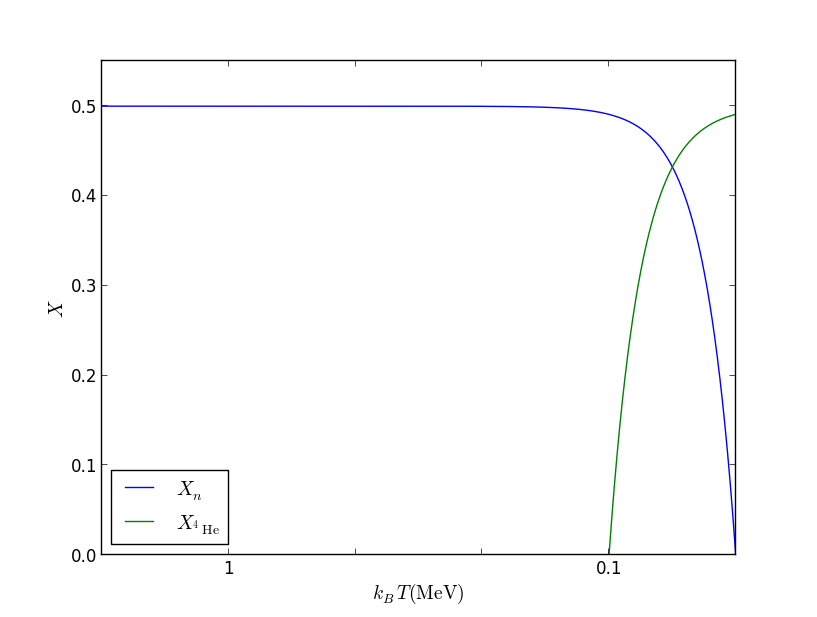
\includegraphics[scale=0.7]{Draw/abundances.png}
\label{}
\end{center}
\caption{Fractional abundances $X_i=n_i/(n_i+n_p)$ of neutrons and $^4$He nuclei as a function of the photon temperature $T$, as results from the numerical solution of the abundance equations (\ref{balancenoneq})}
\label{abun}
\end{figure}
This tells us that the neutron abundance starts to drop dramatically after $k_BT\lesssim 0.1$MeV, due to the weak interactions becoming inefficient in producing new neutrons to replace the ones that decay. Our only hope for forming heavier nuclei, then, is that by this time strong nuclear processes are efficient enough to bind the protons with the neutrons that are left. This is done mainly via the strong process
\begin{equation}
p+n\leftrightarrow D + \gamma
\end{equation}
Where $D$ indicates deuterium, a nuclear bound state between a neutron and a proton. When this reaction is at equilibrium, the deuterium abundance has to obey the thermodynamic equation
\begin{equation}
\label{deuterium}
\frac{n_D}{n_nn_p}=\frac{3}{4}\left(\frac{m_Dh^2}{2\pi k_Bm_nm_p T}\right)^{3/2}e^{(m_n+m_p-m_D)c^2/k_BT}
\end{equation}
Where $B_D=m_n+m_p-m_D=2$MeV is the binding energy of deuterium; for the purpose of this section we will make the crude estimate (for $k_BT\lesssim 0.1$MeV) $n_n\sim n_p \sim\eta_b n_\gamma$. With $n_\gamma \propto T^3$ and $\eta_b\approx 10^{-9}$ is measured from CMB experiments which tell us that there are roughly one billion photons for every baryon in the universe. This allows us to write the approximate equation, starting from (\ref{deuterium})
\begin{equation}
\frac{n_D}{n_p}\sim \eta_b\left(\frac{k_B T}{m_p c^2}\right)^{3/2}e^{B_D/T}
\end{equation}
If we try to see when a substantial amount of deuterium is produced we try to solve this equation for $T$ setting $n_D/n_p=1$ and, again using numerical methods, we get that this happens when $k_B T\approx k_B T_{nucl}=0.07$\,MeV. This corresponds to a redshift $1+z_{nucl}=\frac{T_{nucl}}{T_{CMB}}\approx 2\cdot 10^8$ which translated in time in the $\Lambda$CDM model corresponds to 3 minutes after the Big Bang. We can consider ourselves very lucky then: our universe is made in such a way that the strong nuclear interaction is efficient enough to store most of the neutrons into deuterium in just three minutes, just about in time before all the neutrons decay (which occurs after 15 minutes). If we look again at Figure \ref{abun} we see that that at this time the neutron proton fraction has dropped roughly to $n_n/n_p=1/7$. Now that the neutrons are safely stored into deuterium, the following reactions can occur to produce a heavier nucleus, helium 4, which is formed via
\begin{equation}
D+D \rightarrow n + ^3\mathrm{He}
\end{equation}
\begin{equation}
^3\mathrm{He}+D \rightarrow p + ^4\mathrm{He}
\end{equation}
Helium for is a very stable nucleus, with a binding energy of $B_{^4\mathrm{He}}=28$MeV and it takes about 20 minutes to accumulate in a substantial fraction; once the helium production is over, our current estimates state that helium can account for the 25\% of the mass of baryonic (non dark) matter. These processes of primordial nucleosynthesis cannot form nuclei which are heavier than helium because formation processes like 
\begin{equation}
^4\mathrm{He} + ^4\mathrm{He} +^4\mathrm{He} \rightarrow ^{12}\mathrm{C}
\end{equation}
which can form carbon (the next stable nucleus), require a much bigger helium abundance than 25\% in order to be efficient. For these heavier elements to be formed we have actually to wait for the first collapsed structures to form; when the first stars are formed, carbon can be produced via thermonuclear fusion processes which occur in the core of stars. 
\subsection{The origin of the CMB}
In the previous paragraph we saw that the first light nuclei (which consist in deuterium and helium 4) form respectively after 3 and 20 minutes via strong interactions, solving the problem weak interactions may cause when making the neutron decay with a lifetime of 15 minutes. What is the next step? At this stage in the life of the universe, photons are still tigthly coupled to charged matter, which includes electrons and charged nuclei. After nucleosynthesis, nothing really interesting really happens to this ensemble of particles,which consists in a hot plasma of nuclei and electrons not bound together, immersed in this sea of photons, cooling down as the universe expands. To wait for something actually interesting to happen actually we have to wait other 300,000 years, after which the universe has cooled a sufficient amount to allow electrons bind with protons and charged nuclei to form neutral atoms; this epoch is called \textit{recombination}. In a very similar way as neutrons and protons combine via 
strong nuclear interactions to form deuterium nuclei, protons and electrons can combine to form neutral hydrogen atoms via the electromagnetic reaction
\begin{equation}
p+e^-\leftrightarrow H + \gamma
\end{equation}
An important difference with the previous process is that the binding energy of the hydrogen atom $B_H=m_e+m_p-m_H=13.6$eV is much lower than the binding energy of deuterium nuclei; this is why it's much easier to break an electromagnetic electron proton bond, and a much lower temperature is required for this bond to resist and hold atoms together. Following the guideline of equation (\ref{deuterium}), when the reaction is at equilibrium, we can write a similar relation for electron and hydrogen abundances
\begin{equation}
\frac{n_H}{n_en_p}=\left(\frac{m_Hh^2}{2\pi k_Bm_em_p T}\right)^{3/2}e^{T^*/T}
\end{equation}
With $T^*=B_H/k_B=1.6\cdot 10^5$\,K; now, if we define the ionized fraction of hydrogen $x$ as $n_p=x(n_H+n_p)$ and if we make the simplification $n_e\sim n_p\sim \eta_b n_\gamma$, we can derive a simplified equation for $x$ as a function of temperature, in an analogous way as we did before we did before
\begin{equation}
\frac{1-x}{x^2}\approx 10^{-8}\left(\frac{k_BT}{m_ec^2}\right)^{3/2}e^{T^*/T}
\end{equation}
To get an idea on when recombination occurs, we want to see at which temperature the ionized fraction drops very low, and the hydrogen atoms are dominating in number over the unbound protons; if we set a reference as $x+10^{-3}$, we have to solve for $T$ the equation
\begin{equation}
\left(\frac{k_BT}{m_ec^2}\right)^{3/2}e^{T^*/T}=10^{14}
\end{equation}
Again we can use a computer to do this, but a good approximation, just to set the order of magnitudes is the following
\begin{equation}
T(x=10^{-3})\equiv T_{rec}\approx \frac{T^*}{14\ln{10}+\frac{3}{2}\ln{\left(\frac{m_ec^2}{k_BT^*}\right)}}\approx 3000\, \mathrm{K}
\end{equation}
When the temperature drops below this value, the reactions that keep the photons coupled to charged matter cease to be effective, photons finally decouple and free stream all over the place without interacting, just like the neutrinos, and eventually they reach us, where we detect them with telescopes. This free streaming signal that we see is the Cosmic Microwave Background and it is one of the most important and succesful predictions of modern cosmology; when this radiation background originated, the universe was a big blackbody with a temperature of 3000\,K, which eventuallly cooled down till today, when the measured temperature is just 2.78\,K. This tells us that recombination (or photon decoupling) occurred at a redshift $1+z_{rec}=\frac{T_{rec}}{T_{CMB}}\approx 1000$, which in the $\Lambda$CDM model corresponds to 300,000 years after the big bang.  
\subsection{Why is the CMB so important?}
In this chapter we made a quick outline of the thermal history the universe underwent from the Big Bang to today: we saw that, after it began very hot, eventually it cooled down, the first deuterium nuclei were formed in three minutes, helium was formed in 20 minutes and it took 300,000 years to see the first neutral hydrogen atoms. At this precise time, the CMB was originated: this means that, since the CMB photons do not interact with matter from then to today, this microwave background is an accurate snapshot on how the universe was when it was only 300,000 years old (today the universe is 10 billion years old); in particular an accurate sky map of the CMB captures all the tiny inhomogeneities in the universe's density field that were present at the time, and that we believe are responsible for gravitational collapse and the formation of galaxies, stars and planets. The presence and growth of these inhomogeneities (which are deviations from the homogeneous Friedmann model) will be the subject of next 
lecture.


\chapter{Gravitational collapse and the large-scale structure of the universe}

In the previous lectures our study of cosmology has been restricted by the assumptions of homogeneity and isotropy, as stated in the cosmological principle. We know, however, that the cosmological principle is an approximate law. At present times, the universe is homogeneous and isotropic only on distance scales larger than of order 100 Mpc. However, we will see that there is strong evidence that the early universe was very homogeneous and isotropic on all scales, not just on sufficiently large scales. It follows that as the universe evolved, it experienced a loss of homogeneity on small scales. The goal of this lecture is to study the mechanism responsible for this loss of homogeneity, namely gravitational collapse.

\section{Large-scale structure}

Before beginning our study of gravitational collapse, we will discuss in this section the large-scale structure of the universe. As we briefly mentioned in chapter 6, structure formation is the phase in the thermal history of the universe in which the matter (which, after recombination, is composed of neutral atoms and dark matter) begins to form lumps of gas as a result of gravity. These lumps grow larger and denser as the universe evolves, eventually forming the first stars and galaxies. Our discussion of structure formation will be very qualitative, as many of the details of this phase are not yet fully understood, although a lot of progress has been made during the last decade with the help of powerful computer simulations.

The cosmic microwave background (CMB) gives us a snapshot of the universe when it had an age of $t_{\mathrm{rec}}\approx 380,000$ years (with a corresponding redshift of $z_{\mathrm{rec}}\approx1100$). By observing the temperature of the CMB as a function of the direction in the sky, cosmologists have been able to conclude that, at the time of recombination, the universe was homogeneous {\it on all scales} to one part in $10^5$. This statement can be written as follows:
\begin{equation} \label{eq:cmb_densitybound}
\left| \frac{\rho_r(\mathbf{r},t_{\mathrm{rec}})-\bar{\rho}_r(t_{\mathrm{rec}})}{\bar{\rho}_r(t_{\mathrm{rec}})} \right| \lesssim 10^{-5}.
\end{equation}
Here $\rho_r(\mathbf{r},t_{\mathrm{rec}})$ denotes the photon energy density as a function of position $\mathbf{r}$ evaluated at the time of recombination, $t=t_{\mathrm{rec}}$, whereas $\bar{\rho}_r(t_{\mathrm{rec}})$ denotes the average of $\rho_r(\mathbf{r},t_{\mathrm{rec}})$ over all space. What equation (\ref{eq:cmb_densitybound}) shows is that the difference between the actual density and the average density is never larger than $10^{-5}$ times the average density. In other words, the departure from perfect homogeneity (in which case we would have $\rho_r(\mathbf{r},t_{\mathrm{rec}})=\bar{\rho}_r(t_{\mathrm{rec}})$ for all $\mathbf{r}$) is never larger than about one part in $10^5$. The universe was therefore very homogeneous on all scales during the time of recombination.

Today the universe is also very homogeneous, but only on distance scales of order 100 Mpc and larger. On smaller scales we observe {\it structures}, which range from planets and stars to galaxy clusters and superclusters. The structures that are relevant to astrophysics and cosmology are shown in the following table:
\begin{table}[ht]
\begin{center}
\begin{tabular}{p{5cm} l l} \hline\hline
Structures & Scales  \\ \hline
Planets & $10^4-10^5$ km \\
Stars & $10^6-10^8$ km \\
Stellar clusters & $10-100$ pc \\
Galaxies & $1-100$ kpc \\
Galaxy clusters & $1-10$ Mpc \\
Galaxy superclusters & $50-100$ Mpc \\ \hline\hline
\end{tabular}
\end{center}
\end{table}

Galaxy clusters are collections of a few hundreds of galaxies, while galaxy superclusters are collections of several clusters of galaxies. Of course, there exist all kinds of structures smaller than planets (mountains, rocks, cells, etc.), but the important point is that we do not observe structures larger than galaxy superclusters. As we will see in a later lecture, this observation provides an important constraint on the nature of dark matter. In the following we will briefly study the main properties of clusters and superclusters of galaxies.

\subsubsection{Galaxy clusters}

Galaxy clusters are groups of galaxies interacting gravitationally. Most clusters contain a few hundreds of galaxies, although some may contain as few as 100 galaxies or less while the largest ones contain as many as 1000 galaxies or more.\footnote{Collections of 50 or less galaxies are usually classified as galaxy groups.} The total mass of a typical cluster ranges from $10^{14}$ to $10^{15}$ solar masses, of which only about $3\%$ is contained in galaxies (although this number may be larger for small clusters and galaxy groups). The rest of the mass is contained in the intergalactic gas (about $12\%$) and in the dark matter (about $85\%$). The average speeds of the galaxies in clusters (measured with respect to the center of mass of the cluster) are in the order of $1000$ km/s (for comparison, the speed of the Sun relative to center of the Milky Way is around $220$ km/s).
\begin{figure}[ht]
\begin{center}
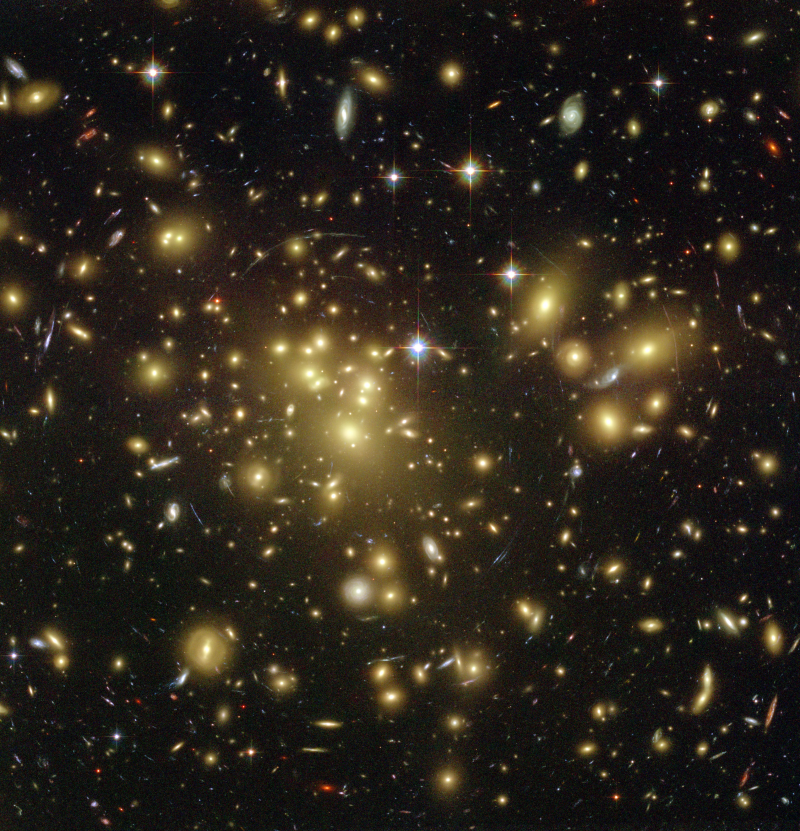
\includegraphics[scale=1.2]{Draw/lec8_1.png}
\end{center}
\caption{Galaxy Cluster Abell 1689 (Image credit: HST, H.\ Ford, JHU)}
\label{fig:lec8_1}
\end{figure}

An important property is that galaxy clusters are in {\it virial equilibrium}. A system in virial equilibrium is one which is neither contracting nor expanding, and which satisfies the virial theorem:
\begin{equation} \label{eq:virial_thm}
\langle E_{\mathrm{pot}}\rangle +2\langle E_{\mathrm{kin}}\rangle =0.
\end{equation}
In this equation $\langle E_{\mathrm{pot}}\rangle$ denotes the average potential energy of the cluster. Since galaxy clusters have roughly spherical shapes (there are exceptions though), we can in general write
\begin{equation} \label{eq:avg_epot}
\langle E_{\mathrm{pot}}\rangle = -\alpha \frac{GM^2}{R},
\end{equation}
where $G$ is Newton's gravitational constant, $M$ is the total mass of the cluster, and $R$ is the radius of the cluster; $\alpha$ is a dimensionless constant of order 1, whose precise value depends on the mass distribution of the cluster.\footnote{As an example, a uniform sphere of mass $M$ and radius $R$ would have $\alpha=3/5$.} On the other hand, $\langle E_{\mathrm{kin}}\rangle$ denotes the average kinetic energy of the cluster, which is given by
\begin{equation} \label{eq:avg_ekin}
\langle E_{\mathrm{kin}}\rangle = \frac{1}{2}M\langle v^2\rangle,
\end{equation}
where $\langle v^2\rangle$ is the average squared speed of the galaxies in the cluster.

If we apply the virial theorem (\ref{eq:virial_thm}), using eqs.\ (\ref{eq:avg_epot}) and (\ref{eq:avg_ekin}), we obtain
\begin{equation}
-\alpha \frac{GM^2}{R}+M\langle v^2\rangle=0,
\end{equation}
\begin{equation}
\Rightarrow~~~~ M=\frac{\langle v^2\rangle R}{\alpha G}.
\end{equation}
This last result is very useful, as it provides a formula for computing the total mass of the cluster, $M$, from the knowledge of $\langle v^2\rangle$, $R$, and $\alpha$. The average squared speed $\langle v^2\rangle$ can be measured directly by observing the Doppler redshift in the emission spectra of the galaxies in a cluster. Similarly, the radius $R$ of a cluster can be measured directly as long as the cluster is not too distant. The constant $\alpha$ is difficult to measure in general, but since we know that it is always of order 1, its precise value is not needed in order to get a rough estimate for the mass $M$.

\subsubsection{Galaxy superclusters}

Galaxy superclusters are collections of several (roughly between 5 and 15) rich clusters of galaxies, plus several dozens of galaxy groups.\footnote{The Local Group (the galaxy group that contains the Milky Way) is part of the Virgo supercluster.} Typical sizes are between 50 and 100 Mpc, although the largest ones can extend to around 200 Mpc. The average separation between superclusters is about 150 Mpc, which has the same order of magnitude of the size of a typical supercluster.\footnote{Compare this fact with the case of stars: the average separation between stars in a galaxy is of order $10^{13}$ km, while the typical size of a star is around $10^6$ km.} The regions between superclusters, which contain very few galaxies, are known as {\it voids}.

Superclusters are {\it not} in virial equilibrium. This is because superclusters are currently undergoing gravitational collapse, meaning that they are still in the process of forming. This is in contrast to galaxy clusters, most of which have finished forming at the present time, and have subsequently achieved virial equilibrium. A useful timescale to distinguish the different structures in the universe is the {\it virialization time}, which is the time lapse from the beginning of gravitational collapse to the time when the system achieves virial equilibrium. The following table shows the virialization times for the large-scale structures:
\begin{table}[ht]
\begin{center}
\begin{tabular}{p{5cm} l l} \hline\hline
Structures & Virialization time  \\ \hline
Galaxies & $10^8$ years \\
Galaxy clusters & $10^9$ years \\
Galaxy superclusters & $10^{10}-10^{11}$ years \\ \hline\hline
\end{tabular}
\end{center}
\end{table}

Comparing these times with the age of the universe ($1.4\times10^{10}$ years), we understand why superclusters are still, at the present time, undergoing gravitational collapse: they simply have not had enough time to achieve a state of virial equilibrium.

The fact that galaxy superclusters are still under formation implies that they can have quite irregular shapes. Unlike galaxy clusters, most of which (especially the rich ones) have roughly spherical shapes, superclusters can have spherical, elongated (filaments), or flattened (walls) shapes. These irregularities give rise to a web-like structure of the universe on its largest scales (fig.\ \ref{fig:lec8_2}).
\begin{figure}[ht]
\begin{center}
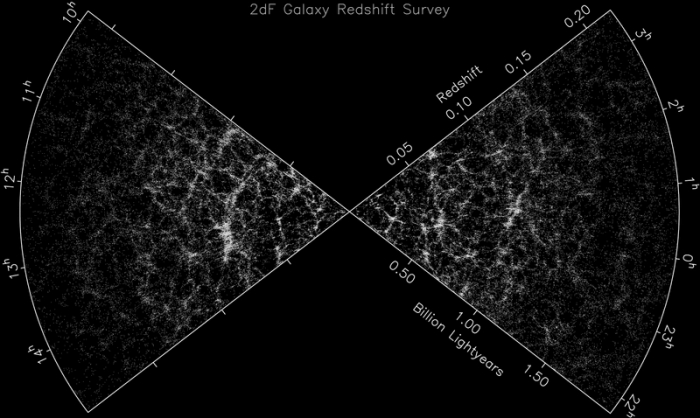
\includegraphics[scale=0.4]{Draw/lec8_2.png}
\end{center}
\caption{The large-scale structure of the universe (Image credit: 2dF Galaxy Redshift Survey)}
\label{fig:lec8_2}
\end{figure}


\section{Gravitational collapse}

We have seen that at the end of recombination the energy content of the universe is formed by neutral particles only: photons, neutrinos, dark matter, and baryonic matter in the form of neutral atoms.\footnote{Dark energy does not play an important role until much later times.} The subsequent evolution is different for each of these four particle species. In this section we will focus on the evolution of the baryonic matter density, but we will comment on what happens to the other species at the end of the section.

After recombination, the initial inhomogeneities in the baryonic matter begin to grow as a result of gravity. Since the gravitational attraction is stronger for larger densities, initially overdense regions start drawing matter from underdense regions. This has the consequence that the density in overdense regions increases in time, while the density in underdense regions decreases in time (see fig.\ \ref{fig:lec8_3}). This is the essence of gravitational collapse.
\begin{figure}[ht]
\begin{center}
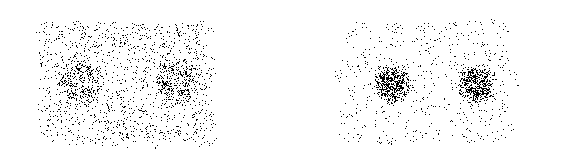
\includegraphics[scale=0.8]{Draw/lec8_3.png}
\end{center}
\caption{Gravitational collapse}
\label{fig:lec8_3}
\end{figure}

Our goal in this section is to describe gravitational collapse in a mathematical way. To do this, we begin by defining the {\it density fluctuation} as follows:
\begin{equation} \label{eq:dens_fluct}
\delta(\mathbf{r},t)=\frac{\rho(\mathbf{r},t)-\bar{\rho}(t)}{\bar{\rho}(t)},
\end{equation}
where $\rho(\mathbf{r},t)$ denotes the mass density of the matter as a function of position $\mathbf{r}$ and time $t$, and $\bar{\rho}(t)$ denotes the average of $\rho(\mathbf{r},t)$ over space.\footnote{We could have also defined $\rho(\mathbf{r},t)$ as the energy density of the baryonic matter, since for nonrelativistic matter the only difference between mass density and energy density is a factor of $c^2$, which would cancel in eq.\ (\ref{eq:dens_fluct}).} An overdense region is one where the local density is larger than the average density, and so $\delta(\mathbf{r},t)>0$ in such a region. Similarly, an underdense region is one where the local density is smaller than the average density, meaning that $\delta(\mathbf{r},t)<0$.

Let us consider a spherical region that is small enough so that we can approximate it as being homogeneous (see fig.\ \ref{fig:lec8_4}). This means that, in this region, we can approximate $\rho(\mathbf{r},t)\approx \rho(t)$, which also implies that $\delta(\mathbf{r},t)\approx \delta(t)$. We will further assume that the rate at which $\delta(t)$ changes in time is much larger than the rate at which the average density $\bar{\rho}(t)$ changes (this is equivalent to neglecting the effects of the Hubble expansion; we will consider these effects later). This means that we can approximate the average density to be constant in time, $\bar{\rho}(t)\approx \bar{\rho}$.
\begin{figure}[ht]
\begin{center}
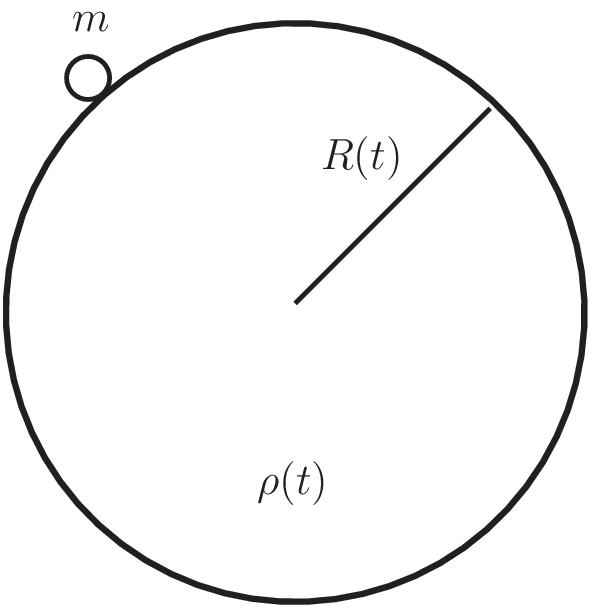
\includegraphics[scale=0.3]{Draw/lec8_4.png}
\end{center}
\caption{Gravitational collapse}
\label{fig:lec8_4}
\end{figure}

Let the mass of the spherical region be $M$, and let its radius be $R(t)$ (which changes in time as a result of gravitational collapse). Consider a small particle of mass $m$ on the boundary of the spherical region. The force felt by the particle is given by Newton's gravitational law:
\begin{equation} \label{eq:force1}
F=-\frac{G(\Delta M)m}{R(t)^2},
\end{equation}
where $\Delta M$ is the excess mass of the sphere relative to the medium, that is,
\begin{equation}
\begin{split}
\Delta M&=\left(\rho(t)-\bar{\rho}\right)V(t)\\
&=\left(\frac{\rho(t)-\bar{\rho}}{\bar{\rho}}\right)\bar{\rho}\left(\frac{4\pi}{3}R(t)^3\right)\\
&=\frac{4\pi}{3}\bar{\rho} R(t)^3\delta(t),
\end{split}
\end{equation}
where $V(t)$ is the volume of the spherical region, and in the last line we used eq.\ (\ref{eq:dens_fluct}). Notice that the position of the particle relative to the center of the sphere is precisely $R(t)$, and so the acceleration of the particle equals $\ddot{R}(t)$, the second time derivative of $R(t)$. By Newton's second law we then have that the force on the particle is given by
\begin{equation} \label{eq:force2}
F=m\ddot{R}(t).
\end{equation}
Combining eqs.\ (\ref{eq:force1}) and (\ref{eq:force2}) we obtain
\begin{equation}
m\ddot{R}(t)=-\frac{Gm}{R(t)^2}\left(\frac{4\pi}{3}\bar{\rho}R(t)^3\delta(t)\right),
\end{equation}
\begin{equation} \label{eq:grav_coll1}
\Rightarrow~~~~ \frac{\ddot{R}(t)}{R(t)}=-\frac{4\pi G\bar{\rho}}{3}\delta(t).
\end{equation}
On the other hand, we know that we can relate the density of the sphere to its radius, since the total mass $M$ is constant. Explicitly, we have
\begin{equation}
\begin{split}
M&= \rho(t)V(t)\\
&=\left(\frac{\left(\rho(t)-\bar{\rho}\right)+\bar{\rho}}{\bar{\rho}}\right)\bar{\rho}\left(\frac{4\pi}{3}R(t)^3\right)\\
&=\frac{4\pi}{3}\bar{\rho} \left(1+\delta(t)\right)R(t)^3,
\end{split}
\end{equation}
\begin{equation}
\Rightarrow~~~~ R(t)^3=\left(\frac{3M}{4\pi\bar{\rho}}\right)\frac{1}{\left(1+\delta(t)\right)},
\end{equation}
\begin{equation} \label{eq:grav_coll2}
\Rightarrow~~~~ R(t)=\left(\frac{3M}{4\pi\bar{\rho}}\right)^{1/3}\frac{1}{\left(1+\delta(t)\right)^{1/3}}.
\end{equation}
Now, remember that our goal is to study the evolution of inhomogeneities after recombination. From our discussion at the beginning of the lecture, we know that the relative size of these inhomogeneities was very small. In other words, $\delta(\mathbf{r},t)\ll1$ at the early stages of gravitational collapse.\footnote{Of course, eventually $\delta(\mathbf{r},t)$ will become large, which is in fact what we observe at the present time. The analysis in this case becomes much more complicated and is usually studied with the help of computer simulations.} Under this assumption we can approximate
\begin{equation}
\frac{1}{\left(1+\delta(t)\right)^{1/3}}\approx 1-\frac{1}{3}\delta(t).
\end{equation}
(Try to show this if you know about Taylor's theorem.) From eq.\ (\ref{eq:grav_coll2}) we then find the approximate relation
\begin{equation} \label{eq:grav_coll3}
R(t)=\left(\frac{3M}{4\pi\bar{\rho}}\right)^{1/3}\left(1-\frac{1}{3}\delta(t)\right).
\end{equation}
If we now take the second time derivative of this last equation we get
\begin{equation} \label{eq:grav_coll4}
\ddot{R}(t)=-\left(\frac{3M}{4\pi\bar{\rho}}\right)^{1/3}\frac{1}{3}\ddot{\delta}(t).
\end{equation}
From eqs.\ (\ref{eq:grav_coll3}) and (\ref{eq:grav_coll4}) we obtain
\begin{equation}
\begin{split}
\frac{\ddot{R}(t)}{R(t)}&=-\frac{1}{3}\ddot{\delta}(t)\frac{1}{\left(1-\frac{1}{3}\delta(t)\right)}\\
&\approx -\frac{1}{3}\ddot{\delta}(t),
\end{split}
\end{equation}
where the last approximation follows because $\ddot{\delta}(t)$ is already a small quantity, and so we can safely neglect the factor of $\delta(t)$ in the denominator. In other words, we are working to first order in the function $\delta(t)$ and its derivatives. Finally, if we plug the last result into eq.\ (\ref{eq:grav_coll1}) we obtain
\begin{equation}
-\frac{1}{3}\ddot{\delta}(t)=-\frac{4\pi G\bar{\rho}}{3}\delta(t),
\end{equation}
\begin{equation} \label{eq:grav_coll5}
\Rightarrow~~~~ \ddot{\delta}(t)=4\pi G\bar{\rho}\delta(t).
\end{equation}
Eq.\ (\ref{eq:grav_coll5}) is a differential equation for the function $\delta(t)$. Its solution is given by
\begin{equation} \label{eq:delta_sol}
\delta(t)=Ce^{t/t_{\mathrm{dyn}}},
\end{equation}
where $C$ is a constant that has to be computed from the initial conditions, and we defined the {\it dynamical timescale}
\begin{equation}
t_{\mathrm{dyn}}\equiv \frac{1}{\sqrt{4\pi G \bar{\rho}}}.
\end{equation}

%\par\vspace{\baselineskip}
\newpage

{\bf Exercise.}
\begin{itemize}
\item [(a)] Find the second time derivative of $\delta(t)$ from the solution (\ref{eq:delta_sol}), and verify that eq.\ (\ref{eq:grav_coll5}) is satisfied.
\item [(b)] Suppose that the initial value of the density fluctuation is $\delta(t=0)=10^{-3}$. Find the value of $\delta(t)$ at $t=10t_{\mathrm{dyn}}$.
\end{itemize}

\par\vspace{\baselineskip}

Notice that the constant $C$ in eq.\ (\ref{eq:delta_sol}) could be positive or negative. Clearly, $C$ will be positive for an initially overdense inhomogeneity; what eq.\ (\ref{eq:delta_sol}) then tells us is that $\delta(t)$ will always be positive, and that it will grow larger in time. Similarly, for an initially underdense inhomogeneity $C$ will be negative, and so $\delta(t)$ will always be negative and it will grow larger (it will become more negative) in time. This confirms what we qualitatively discussed at the beginning of the section: initially overdense regions become more and more overdense in time, while initially underdense regions become more and more underdense in time.

Another important thing that eq.\ (\ref{eq:delta_sol}) tells us is that $\delta(t)$ will become large on timescales of the order of $t_{\mathrm{dyn}}$. This conclusion has a caveat however, namely that so far we have only considered gravity. But there are two other effects that act {\it against} gravitational collapse: one is the pressure and the other is the Hubble expansion. In the following we will study these effects in order to see how they modify the above conclusions.

\subsection{Effects of pressure}

We have seen that, in the absence of any other effects apart from gravity, matter will tend to collapse exponentially fast. Of course, this is not what we observe; planets, stars, and galaxies, for instance, are perfectly stable systems. There must be some force, then, that opposes gravity in such a way that the net force is zero and the system can remain in stable equilibrium. This force, of course, is provided by the pressure.

Let us consider a spherical cloud of gas with initial radius $R$. As soon as gravitational collapse starts, the gas in the system will attempt to stop the contraction by building up a pressure gradient; it is this gradient that gives rise to an outward-directed force that opposes gravity. As the cloud contracts the gravitational force on each layer becomes stronger, and so the pressure gradient has to become steeper in order to stop the collapse. This steepening of the pressure gradient is not instantaneous however, since the ``news'' about the collapse travel at a finite speed through the gas cloud. This speed is given by the {\it sound speed} $c_s$ of the gas, which corresponds to the speed at which pressure perturbations propagate through a given medium. The typical time it takes for the pressure gradient to become sufficiently steep and stop the collapse is given by the {\it pressure timescale}:
\begin{equation}
t_p\equiv \frac{1}{2\pi}\frac{R}{c_s}.
\end{equation}
Notice that $R/c_s$ is nothing but the time it takes for a pressure perturbation to travel, along a straighy line, from the edge of the cloud to the center. The numerical factor of $1/2\pi$ is not really important, and is a result of the fact that pressure perturbations are waves.

The important question is the following: can the cloud of gas build up a pressure gradient quickly enough to stop the collapse? Clearly, to answer this question we need to compare the pressure timescale, $t_p$, with the dynamical timescale, $t_{\mathrm{dyn}}$. Recall that $t_{\mathrm{dyn}}$ is the typical time it takes for an inhomogeneity to grow large, and so we can identify $t_{\mathrm{dyn}}$ as the time for gravitational collapse. If $t_p>t_{\mathrm{dyn}}$ then the pressure in the gas does not act fast enough to halt the contraction; the collapse will then continue until some new effect happens that makes $t_p$ shorter,\footnote{In the case of stars, this new effect corresponds to nuclear fusion, which provides the pressure needed to stabilize the star against gravity.} or until the cloud becomes so dense that a black hole forms.

To stop the collapse and make the system stable, it is then necessary to have $t_p<t_{\mathrm{dyn}}$. This inequality can be written as follows:
\begin{equation}
\frac{1}{2\pi}\frac{R}{c_s}<\frac{1}{\sqrt{4\pi G \bar{\rho}}},
\end{equation}
which implies an upper bound on the radius $R$ of the gas cloud:
\begin{equation} \label{eq:jeans_def}
R< c_s\left(\frac{\pi}{G\bar{\rho}}\right)^{1/2} \equiv \lambda_J.
\end{equation}
This upper bound, $\lambda_J$, is known as the {\it Jeans length}. From this last result we can state the criterion for gravitational collapse in terms of the size of the system. If $R<\lambda_J$, the collapse will be stopped by the pressure and the system will reach a state of equilibrium. If $R>\lambda_J$, the collapse will continue as described above.

Let us next apply these results to the matter inhomogeneities in the universe. Recombination occurs during the matter-dominated epoch, which implies that we can neglect both the radiation density and the dark energy density in the Friedmann equation:
\begin{equation} \label{eq:fried_eq_inhom}
H^2=\frac{8\pi G}{3}\bar{\rho},
\end{equation}
where $H=\dot{a}/a$ is the Hubble parameter. Notice that the Friedmann equation involves the average density $\bar{\rho}$, not the actual matter density $\rho(\mathbf{r},t)$. This is because the Friedmann equation follows from the Einstein equations under the assumption of perfect homogeneity, and therefore corresponds to the leading-order approximation when we move on to study small inhomogeneities. Solving for $\bar{\rho}$ from eq.\ (\ref{eq:fried_eq_inhom}) we can express the dynamical timescale in terms of the Hubble parameter as follows:
\begin{equation}
\begin{split}
t_{\mathrm{dyn}}&=\frac{1}{\sqrt{4\pi G\bar{\rho}}}\\
&=\sqrt{\frac{2}{3}}\frac{1}{H}.
\end{split}
\end{equation}
Expressing also the Jeans length in terms of $H$ gives
\begin{equation} \label{eq:jeans_hubble}
\lambda_J=2\pi\sqrt{\frac{2}{3}}\frac{c_s}{H}.
\end{equation}
Let us first study gravitational collapse at times before recombination during the matter-dominated epoch. During this stage the baryons (atomic nuclei and electrons) are coupled to the photons in a state of thermal equilibrium. Moreover, even though the universe is matter-dominated at this time, the baryon energy density is smaller than the radiation energy density,\footnote{It is because of the dark matter that the universe is matter-dominated at this time.} which implies that the thermodynamic properties of the cosmic plasma will be approximately those of a gas of photons. Now, one can show that the sound speed of a gas of photons is given by\footnote{You may find surprising that the sound speed of a gas of photons is not exactly $c$, since after all the photons in the gas are all moving at the speed of light. However, remember that the sound speed is the speed at which pressure perturbations travel in a fluid, which in general will be smaller than the average speed of the particles that compose the fluid.
}
\begin{equation}
c_s=\frac{c}{\sqrt{3}}.
\end{equation}
Taking this value as the approximate sound speed of the cosmic plasma before recombination, we find from eq.\ (\ref{eq:jeans_hubble}) a corresponding Jeans length of
\begin{equation}
\lambda_J= \frac{2\pi\sqrt{2}}{3}\frac{c}{H}\approx 3\frac{c}{H}.
\end{equation}
Recall that the size of the observable universe is of the order of the Hubble distance $c/H$. What the above equation tells us is that the Jeans length is larger than the observable universe. Although in the above analysis we concluded that inhomogeneities with sizes larger than $\lambda_J$ will collapse gravitationally, we did not take into account the effects of the expansion of the universe. These effects become dominant over the Newtonian gravitational effects precisely on distance scales of the order of $c/H$ and larger. This implies that an inhomogeneity with size $R>\lambda_J\approx 3c/H$ will not actually undergo gravitational collapse. The important conclusion, then, is that baryon inhomogeneities do not grow before recombination.

Let us next see what happens after recombination. The baryons (which now are in the form of neutral atoms) are now completely decoupled from the photons, so the thermodynamic properties of the baryonic matter are not related to those of the photons, as happened before recombination. One can show that the sound speed of the baryonic matter is now given by
\begin{equation} \label{eq:sound_speed2}
c_s=\left(\frac{k_B T}{\bar{m}}\right)^{1/2},
\end{equation}
where $k_B$ is the Boltzmann constant, $T$ is the temperature, and $\bar{m}$ is the average mass of the particles in the baryonic fluid (which after recombination is approximately equal to $1.22$ times the proton mass). Notice that, since $T$ decreases as the universe expands, so does the sound speed. Evaluating at the time just after the end of recombination, one finds the value $c_s\approx1.5\times10^{-5}c$, which corresponds to a Jeans length of
\begin{equation}
\lambda_J\approx 7.7\times10^{-5}\frac{c}{H}.
\end{equation}
In contrast to what happens before recombination, the Jeans length is now much smaller than the Hubble distance. There exist inhomogeneities, then, with sizes larger than $\lambda_J$ (but smaller than $c/H$, so that the Hubble expansion will not be relevant) that will undergo gravitational collapse. This confirms that structure formation only takes place after the end of recombination, as we stated at the beginning of the lecture.

\subsection{Effects of Hubble expansion}

We have already discussed qualitatively how the expansion of the universe acts against gravitational collapse, and in particular, how it prevents inhomogeneities with sizes larger than the Hubble distance from collapsing. The main conclusion of the previous subsection is that an inhomogeneity of size $R$ will undergo gravitational collapse only if
\begin{equation}
\lambda_J<R<\frac{c}{H}.
\end{equation}
If $R<\lambda_J$ then the pressure in the fluid will halt the collapse. If $R>c/H$ then the Hubble expansion will dominate over the Newtonian gravitational attraction and the collapse will not take place.

Our next goal is to find how the density fluctuation $\delta(t)$ evolves in time. We already did this at the beginning of the section by means of a purely Newtonian analysis, finding that $\delta(t)$ increases exponentially fast; we want to see now how the effects of the expansion of the universe change this picture. For this we need to use the Einstein equations, which become quite complicated after one drops the assumption of perfect homogeneity. One can show that the differential equation that determines $\delta(t)$ (assumed to be small) reads
\begin{equation} \label{eq:delta_eq1}
\ddot{\delta}(t)+2H(t)\dot{\delta}(t)=4\pi G\bar{\rho}(t)\delta(t).
\end{equation}
Notice that for $H=0$, i.e.\ in a static universe, we recover the Newtonian equation (\ref{eq:grav_coll5}) as expected. It is convenient to express the average matter density $\bar{\rho}$ in terms of the matter density parameter $\Omega_m$ as follows:
\begin{equation}
\Omega_m(t)=\frac{\bar{\rho}(t)}{\rho_c(t)}=\frac{8\pi G}{3H(t)^2}\bar{\rho}(t),
\end{equation}
\begin{equation}
\Rightarrow~~~~ 4\pi G\bar{\rho}(t)=\frac{3}{2}\Omega_m(t)H(t)^2.
\end{equation}
Using this in eq.\ (\ref{eq:delta_eq1}) we find
\begin{equation} \label{eq:delta_eq2}
\ddot{\delta}(t)+2H(t)\dot{\delta}(t)-\frac{3}{2}\Omega_m(t)H(t)^2\delta(t)=0.
\end{equation}

Let us first solve eq.\ (\ref{eq:delta_eq2}) for the radiation-dominated epoch. During this time the baryons are coupled to the photons, so the density fluctuation $\delta(t)$ corresponds to the dark matter in this case. In a universe dominated by radiation the contribution of the matter to the total energy is negligible, and so $\Omega_m\approx0$. Also, as it was shown in chapter 5, the Hubble parameter for a radiation-dominated universe is given by
\begin{equation}
H(t)=\frac{1}{2t}.
\end{equation}
With these results eq.\ (\ref{eq:delta_eq2}) reduces to
\begin{equation} \label{eq:delta_eq_rad}
\ddot{\delta}(t)+\frac{1}{t}\dot{\delta}(t)=0.
\end{equation}
This equation has the following solution:
\begin{equation}
\delta(t)=C_1\log t,
\end{equation}
where $C_1$ is a constant. Recall that the logarithm is a function that increases very slowly. The above solution then implies that $\delta(t)$ increases very slowly during the radiation-dominated epoch, and so the gravitational collapse of the dark matter occurs very slowly during this stage.

Next, we solve eq.\ (\ref{eq:delta_eq2}) for the matter-dominated epoch, but before recombination. The density fluctuation $\delta(t)$ again is that of the dark matter, since baryons are strongly coupled to photons in the cosmic plasma. In a universe dominated by matter the contributions of the radiation and dark energy are negligible, and so $\Omega_m\approx 1$. From the results of chapter 5 we also know that the Hubble parameter in a matter-dominated universe is given by
\begin{equation}
H(t)=\frac{2}{3t}.
\end{equation}
Using these results in eq.\ (\ref{eq:delta_eq2}) we find
\begin{equation} \label{eq:delta_eq_mat}
\ddot{\delta}(t)+\frac{4}{3t}\dot{\delta}(t)-\frac{2}{3t^2}\delta(t)=0.
\end{equation}
This equation has the following solution:
\begin{equation}
\delta(t)=C_2t^{2/3},
\end{equation}
where $C_2$ is a constant. This result shows that, after the universe becomes matter-dominated (which, remember, occurs before recombination), dark matter inhomogeneities begin to grow as $\delta(t)\propto t^{2/3}$. Notice that this growth rate is much slower than the exponential rate that we found when neglecting the effects of the Hubble expansion.

\par\vspace{\baselineskip}

{\bf Exercise.} The differential equations (\ref{eq:delta_eq_rad}) and (\ref{eq:delta_eq_mat}) are second order equations (they involve second time derivatives), which means that in fact they have two independent solutions.
\begin{itemize}
\item [(a)] Verify that the general solution of eq.\ (\ref{eq:delta_eq_rad}) is given by
\begin{equation}
\delta(t)=C_1\log t+C_1',
\end{equation}
where $C_1$ and $C_1'$ are arbitrary constants.
\item [(b)] Verify that the general solution of eq.\ (\ref{eq:delta_eq_mat}) is given by
\begin{equation}
\delta(t)=C_2t^{2/3}+C_2'\frac{1}{t},
\end{equation}
where $C_2$ and $C_2'$ are arbitrary constants.
\item [(c)] In the above analysis we did not bother with considering these additional solutions ($C_1'$ in part (a), and $C_2'/t$ in part (b)). Why is this justified?
\end{itemize}

\par\vspace{\baselineskip}

Baryon inhomogeneities do not grow before recombination, as we have seen above. But what happens after recombination? The universe is still matter-dominated, and the baryons are now decoupled from the photons, so one may think that we could apply the above analysis to baryons just like we did to dark matter, and conclude that the baryonic density fluctuation grows proportional to $t^{2/3}$ after recombination. In fact, baryon inhomogeneities begin to grow {\it faster} than $\propto t^{2/3}$ (see fig.\ \ref{fig:lec8_5}). This is because, by the end of recombination, the dark matter inhomogeneities have already grown significantly, and so the atoms that form the baryonic matter are attracted to the dark matter structures that have formed by this time. In other words, in the absence of dark matter, baryonic inhomogeneities would grow slower and, in fact, their size at the present time would be much smaller than what observations suggest. Thus, observations of the large-scale structure of the universe provide an 
independent evidence for the existence of dark matter.
\begin{figure}[ht]
\begin{center}
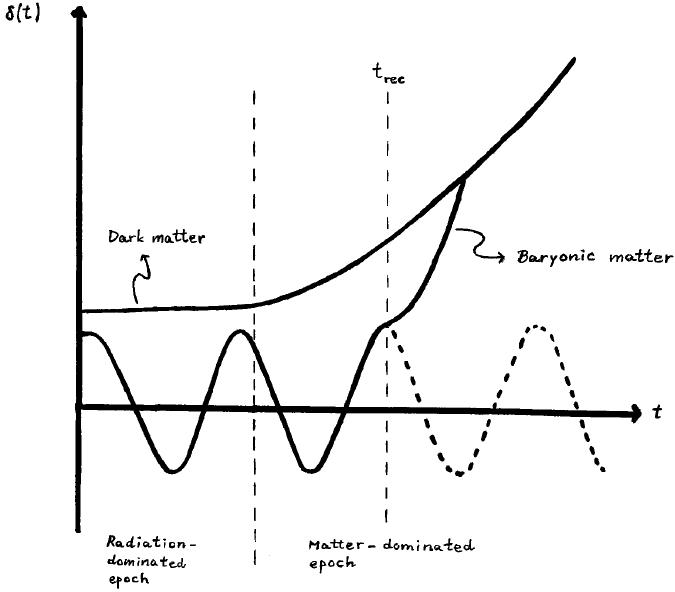
\includegraphics[scale=0.5]{Draw/lec8_5.png}
\end{center}
\caption{Evolution of inhomogeneities}
\label{fig:lec8_5}
\end{figure}

As discussed above, the gravitational collapse may eventually stop due to the effects of pressure. This is in fact what happens to dark matter, which forms the dark matter halos that we (indirectly) observe today around galaxies. Initially, pressure also halts the gravitational collapse of the baryonic matter. However, unlike what happens to dark matter, baryonic matter eventually cools down by emitting radiation. As a consequence, the temperature of a cloud of baryonic gas will decrease in time, and by eq.\ (\ref{eq:sound_speed2}) the sound speed of the gas will decrease as well. Also, we see from eq.\ (\ref{eq:jeans_def}) that the Jeans length will accordingly decrease, which implies that the condition for collapse ($R>\lambda_J$) will eventually be satisfied as the gas continues to cool down. The conclusion is that, for baryonic matter, gravitational collapse will continue until the formation of the first stars takes place.


\chapter{The cosmic microwave background}
The goal of this chapter will be to understand a little bit more quantitatively why the Cosmic Microwave background is so important in the study of cosmology; in particular we want to understand how one can extract meaningful information from the sky temperature measurements of the CMB. As we have seen, the CMB is the radiation leftover from the bigbang, which originated at the epoch of recombination, when the universe became charge neutral and the photons decoupled from matter, free streaming toward us, when we measure them. We measure the temperature of this radiation (in the sense pointed out in Chapter \ref{chp7}) to be $T_{CMB}=2.78$K (see Figure \ref{cmbspectral} for reference). As of now, we have approximated this radiation as uniform all over the sky; in reality, as previously announced, the spatial temperature profile of the CMB is not uniform, but contains very tiny fluctuations of relative order $\frac{\delta T}{T}\approx 10^{-5}$, as you can see in Figure \ref{cmbwmap}, which is a full sky CMB 
map taken by the WMAP satellite 
\begin{figure}
\begin{center}
\includegraphics[scale=0.5]{CMB/wmap}
\label{}
\end{center}
\caption{A full sky map of the Cosmic Microwave Background, from the experiment WMAP: the fluctuations in temperature from red to blue spots have a relative magnitude $\delta T/T\sim 10^{-5}$.  Credit for the image \url{http://apod.nasa.gov/apod/ap030212.html}}
\label{cmbwmap}
\end{figure}
What this map really represents is a (very accurate) snapshot on how the universe was at the time of recombination (i.e. when it was only $t_{rec}\sim 300,000$\,yr old), capturing all the inhomogeneities that were present at that time, and that we believe originated all the collapsed structures (star, galaxies,etc...) that we see today. In this chapter we want to understand better how we can extract cosmological information from the spatial arrangement and size of these inhomogeneities, and what are the physical mechanism that originated them. Before doing this, however, we need to master some useful mathematical tools for analyzing scale dependent variations, namely the basics of Fourier analysis. 

\section{How do we describe inhomogeneities quantitatively?}
\label{fouriersection}
In physics there are plenty of examples where we have to deal with quantities that are non uniform and vary in space; you can think about the temperature profile of a conducting rod (1 dimensional variation), the height of the water ripples on a lake (2 dimensional variations) or the density profile of a gas cloud in the interstellar medium (3 dimensional variation). In the following, we will give a brief summary on how to analyze these different kinds of inhomogeneities. 
\subsection{One dimensional inhomogeneities}
Think about a simple example os outlined before we have a long metal cable fixed at two points; suppose that some physical mechanism acting on this rod makes it oscillate, and each point $x$ on the cable is displaced from its equilibrium position by an amount $y=f(x)$ (at fixed time) with $f$ some function of $x$. Consider the example where $f$ describes a simple harmonic wave, as in Figure \ref{fourier1d} (think of all the lengths expressed in cm)
\begin{figure}
\begin{center}
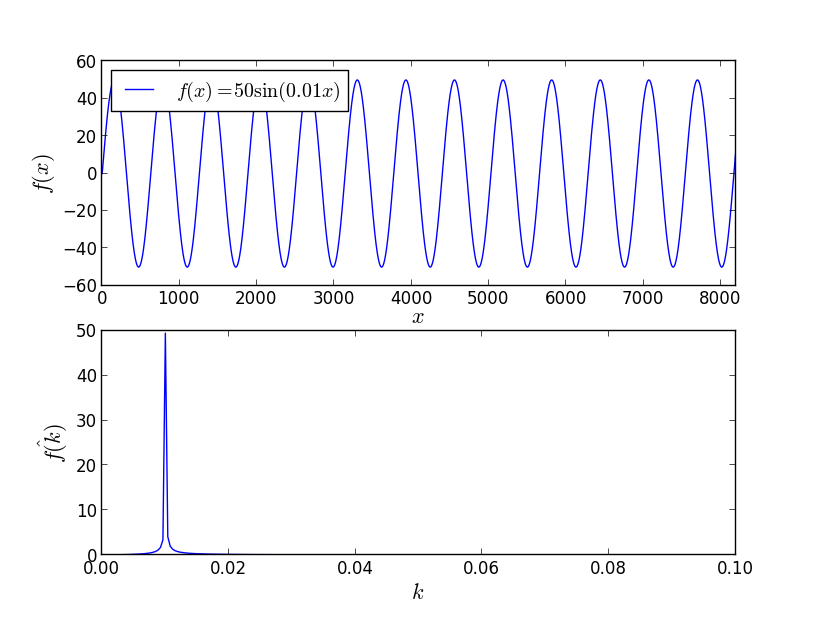
\includegraphics[scale=0.7]{Fourier/1component.png}
\label{}
\end{center}
\caption{The profile of an harmonic wave traveling on a metal cable; the meaningful variations in the cable profile occur on a spatial scale $\lambda=\frac{2\pi}{k}=\frac{2\pi}{0.01}$; the Fourier transform $\hat{f}(k)$ captures this feature}
\label{fourier1d}
\end{figure}
We can see that the inhomogeneities in the cable profile occur on a spatial scale of $\lambda=\frac{2\pi}{0.01}\,\mathrm{cm}\approx 600\,\mathrm{cm}$; if we look on scale lengths much smaller than $600$\,cm we won't notice that the cable profile is inhomogeneous. We will see the inhomogeneities only when we look at scale comparables with $\lambda$; this is precisely what the bottom panel of Figure \ref{fourier1d} tells us: the \textit{Fourier transform} $\hat{f}(k)$ is a function that can be uniquely calculated from the original function $f$ and tells us how much information of $f$ is stored in a scale $\lambda=\frac{2\pi}{k}$. We see that, in this case, all the information is stored in a unique scale $\lambda$ corresponding to a \textit{wavenumber} $k=0.01\mathrm{cm}^{-1}$. The way this Fourier transform is calculated, is by \textit{matching} our original function $f$ with a \textit{template} that contains information in a single scale only (in this case a sine function $\sin{kx}$) 
\begin{equation}
\label{trasf1d}
\hat{f}(k)=\int_0^Lf(x)\sin{(kx)}dx
\end{equation}
When $\hat{f}(k)=0$, it means that our function $f(x)$ doesn't contain any information on the particular spatial scale $\lambda=\frac{2\pi}{k}$; to illustrate the usefulness of this way of analyzing inhomogeneities, consider the following two examples outlined in Figure \ref{fourier23d}
\begin{figure}
\begin{center}
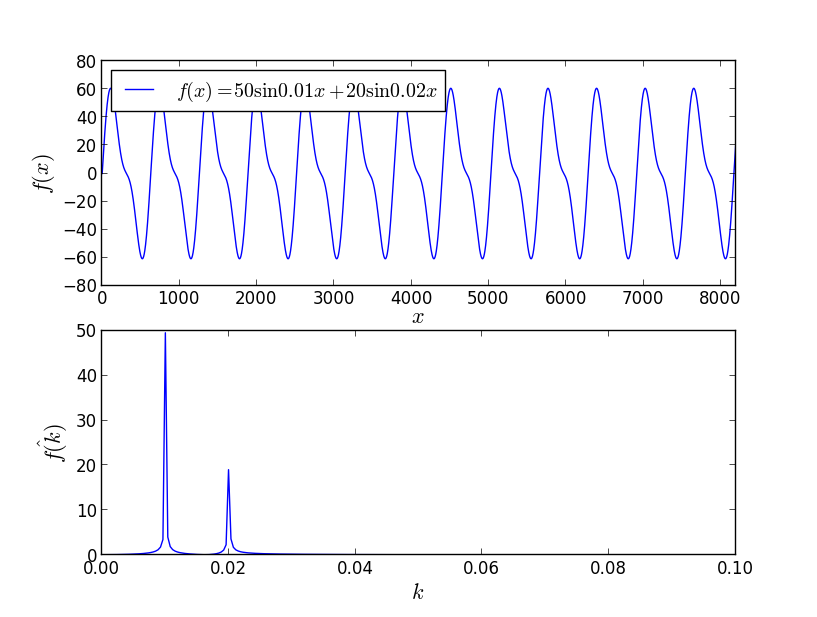
\includegraphics[scale=0.4]{Fourier/2component.png}
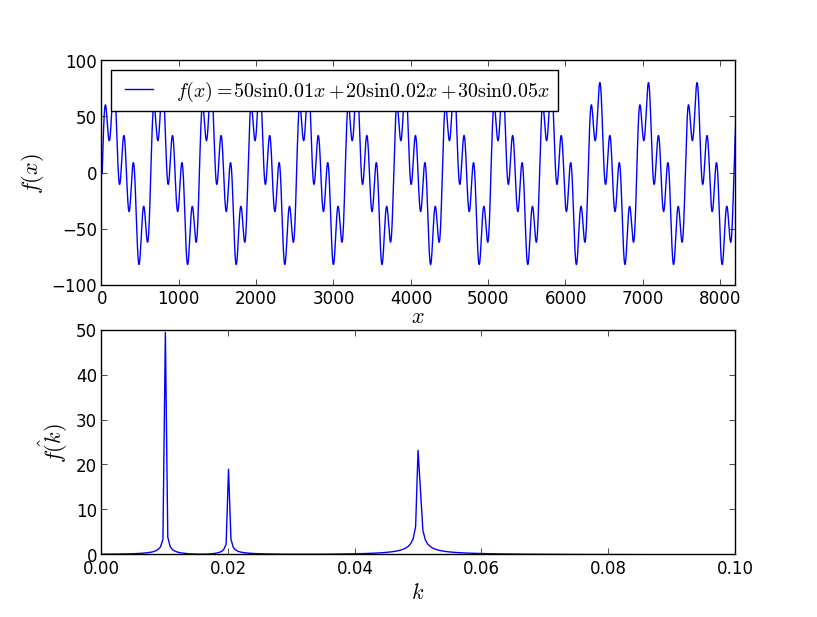
\includegraphics[scale=0.4]{Fourier/3component.png}
\label{}
\end{center}
\caption{Examples of functions whose inhomogeneities contain information on multiple length scales, namely 2(left panel) or 3(right panel)}
\label{fourier23d}
\end{figure}
We immediately see that, even if the cable profiles become messy, this Fourier analysis trick tells us immediately where (in which spatial scales) the relevant information is stored. Fourier analysis can also be quite useful in extracting a signal from a noisy background; consider for example Figure \ref{gaussnoise}
\begin{figure}
\begin{center}
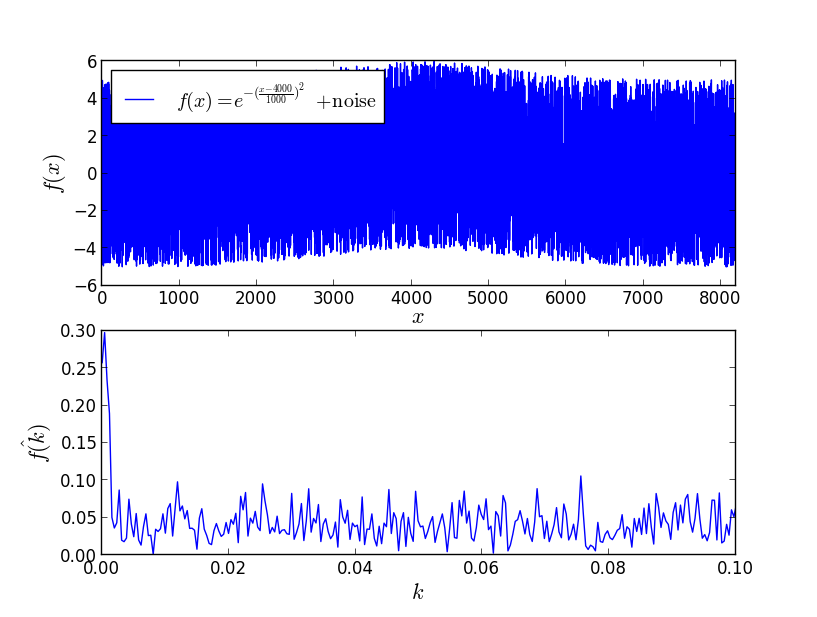
\includegraphics[scale=0.6]{Fourier/gauss+noise.png}
\label{}
\end{center}
\caption{A gaussian peak $f(x)\propto e^{-(x-\mu)^2/2\sigma^2}$ contains information on a length scale $\sigma \gg \lambda_{noise}$, and hence a Fourier analysis is able to separate the signal information from the noise background, which acts on much smaller length scales }
\label{gaussnoise}
\end{figure}
In this case the signal (a gaussian peak) contains information on a scale which is much bigger than the typical scale of the noise; we clearly see this feature in the Fourier transform in Figure \ref{gaussnoise}, which peaks at low $k$ can distinguish clearly the signal contribution from the noise one. We want to extend this concept of one dimensional Fourier analysis to 2d inhomogeneities, with our goal to understand 2 dimensional CMB maps in mind. 
\subsection{Two dimensional inhomogeneities}
\label{2dsection}
In this section, we wish to extends all the concepts of Fourier analysis presented before, but applied to two dimensional systems (for example a two dimensional temperature map of the CMB sky); what we will need is find suitable templates that correspond to a particular spatial scales, and a prescription similar to equation (\ref{trasf1d}) to compare them with the non homogeneous field we wish to analyze. If our 2 dimensional space were to be infinite and flat, we would use templates in the form $\tau_{k_x,k_y}=\sin{ (k_x x)}\sin{(k_y y)}$ in analogy to what we have already done; it turns out however that in the case of the CMB our field of view is neither infinite nor flat. In particular it is the inner surface of a sphere, which we have already seen we can describe in terms of two angular coordinates $(\theta,\phi)$ as in Figure \ref{coordinates}, fixing the radius to $r=1$. What our current experiments do is measuring the temperature profile on sky $T(\mathbf{\hat{n}})=T(\theta,\phi)$ varying the 
direction of observation $\mathbf{\hat{n}}=(\sin \theta \cos \phi,\sin \theta \sin \phi,\cos \theta)$; it turns out that for describing the temperature field $T(\mathbf{\hat{n}})$ the most suitable templates, which encode the scale which we want to extract the information about, are some special functions called \textit{spherical harmonics}. These functions are labelled each by a couple of integer numbers $(l,m)$, where $l=0,1,2,....$ and $-l\leq m \leq l$; to understand to which angular scale each template corresponds, we have to know the fact that
\begin{equation}
Y_{ll}(\theta,\phi)\propto \cos^l\theta \sin{(l\phi)}
\end{equation}
which, if you think about it a little bit, exibits significant variations on an angular scale $\delta \theta \approx \delta\phi \approx \pi/l$. We don't want to go into the details of these spherical harmonics too much, but it can be shown that a similar behaviour holds also for the spherical harmonics with $m\neq l$; for the sake of understanding all we need is know that a spherical harmonic $Y_{lm}$ can serve us as a template to extract information from a sky temperature map $T(\mathbf{\hat{n}}$) on an angular scale $\pi/l=180^\circ/l$. In Figure \ref{sphharmonics} are some examples of sky temperature maps built with only one template (i.e. that contain information on only one angular scale, analogously to Figure \ref{fourier1d}). 
\begin{figure}
\begin{center}
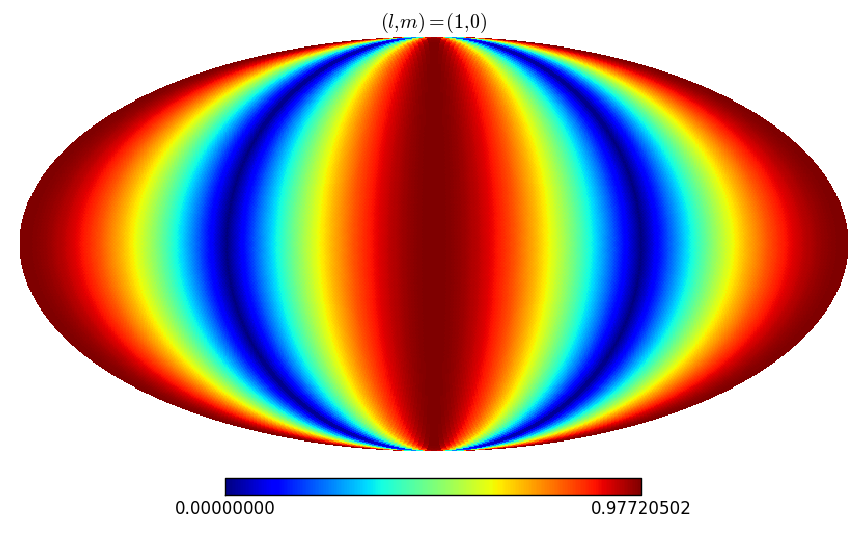
\includegraphics[scale=0.3]{Fourier/(1,0).png}
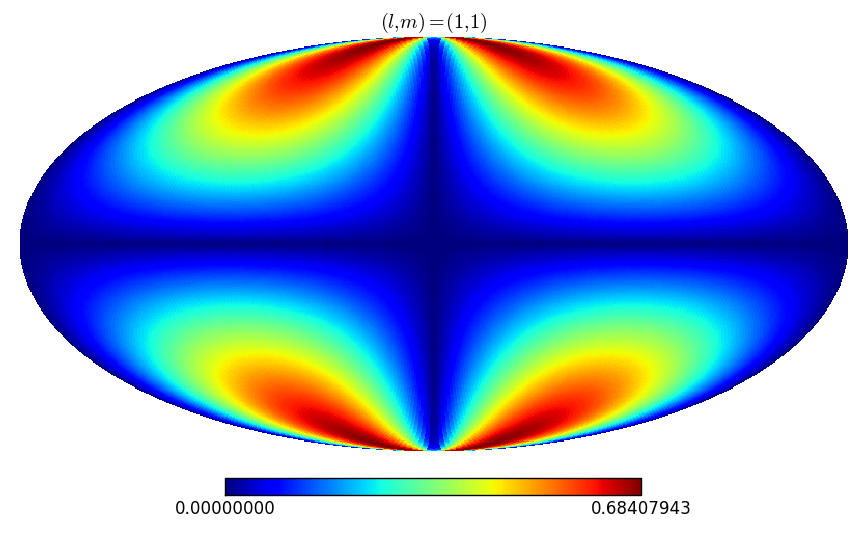
\includegraphics[scale=0.3]{Fourier/(1,1).png}
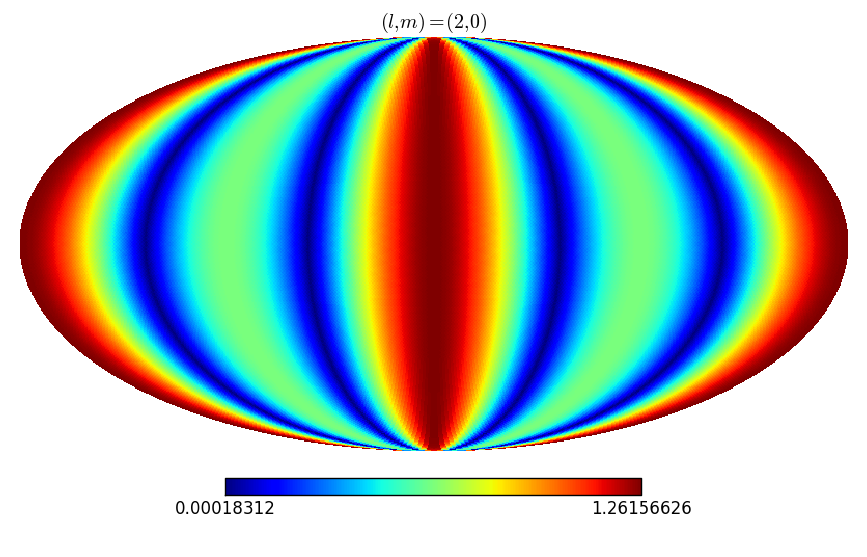
\includegraphics[scale=0.3]{Fourier/(2,0).png}
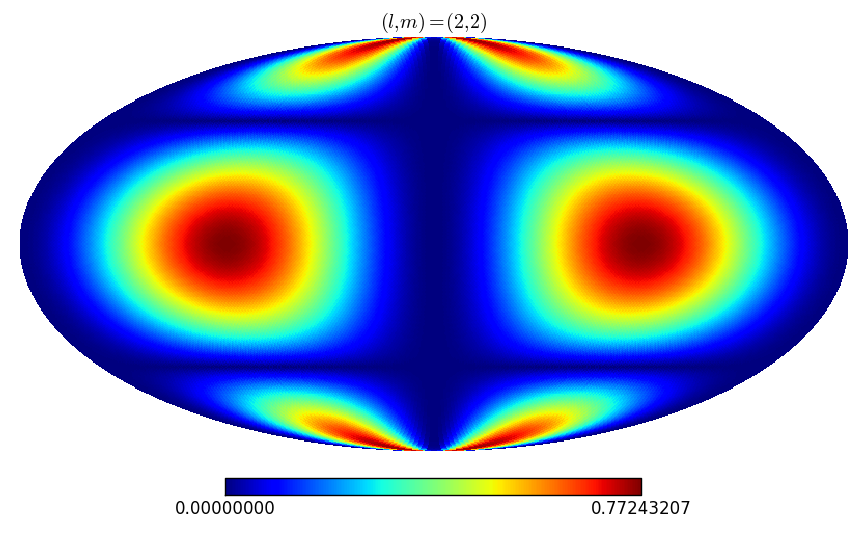
\includegraphics[scale=0.3]{Fourier/(2,2).png}
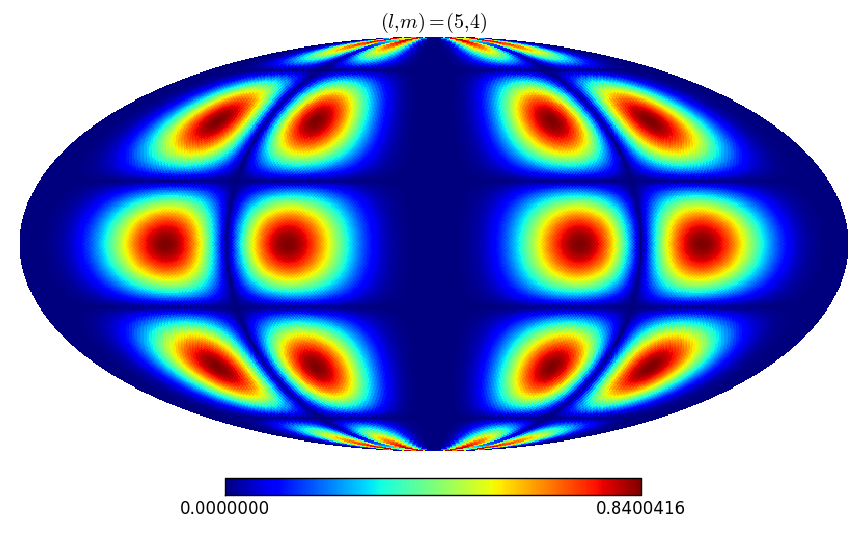
\includegraphics[scale=0.3]{Fourier/(5,4).png}
\includegraphics[scale=0.3]{Fourier/(10,0).png}
\includegraphics[scale=0.3]{Fourier/(10,7).png}
\includegraphics[scale=0.3]{Fourier/(100,50).png}
\end{center}
\caption{Whole sky maps of $Y_{l,m}(\theta,\phi)+Y_{l,-m}(\theta ,\phi)$ in mollweide projection for $(l,m)=(1,0),(1,1),(2,0),(2,2),(5,4),(10,0),(10,7),(100,50)$ 
from left to right, top to bottom}
\label{sphharmonics}
\end{figure}
As you can see increasing $l$ decreases the angular scale of the template, while changing $m$ has to do with the rotational symmetry of the arrangement: $m=0$ means the template is symmetric for rotations along the horizontal axis, which is $\mathbf{\hat{z}}$ in mollweide projection, while $m\neq 0$ introduces a periodic structure in $\phi$ with period $2\pi/m$. One can think of a sky map that contains information on multiple scales, in analogy with Figure \ref{fourier23d}, and think and about an example like Figure \ref{superp}
\begin{figure}
\begin{center}
\includegraphics[scale=0.6]{Fourier/superp.png}
\label{}
\end{center}
\caption{A whole sky map that contains relevant information on three different angular scales, and receives contributions from three templates, $l=2,l=10$ and $l=100$, with relative weights 1,2,1.5}
\label{superp}
\end{figure}
A real world CMB map however won't be so easy to describe, because it will contain information on \textit{all} angular scales (this last example contains information only on three different angular scales); depending on the angular resolution of our experiment, call it $\delta \theta$, we will be able to probe the CMB sky only up to a maximum $l_{max}\sim 180^\circ/\delta \theta$. Depending on how big is the $l_{max}$ we are able to probe, our real CMB sky can look quite different when we image it, as you can see in Figure \ref{simcmbsky}. We will explain this better in the following paragraph. 
\begin{figure}
\begin{center}
\includegraphics[scale=0.3]{CMB/l5.png}
\includegraphics[scale=0.3]{CMB/l50.png}
\includegraphics[scale=0.3]{CMB/l256.png}
\includegraphics[scale=0.3]{CMB/l1024.png}
\end{center}
\caption{Computer simulated CMB temperature maps including information up to a maximum $l_{max}=5,50,256,1024$, left to right, top to bottom}
\label{simcmbsky}
\end{figure}
\subsection{The CMB anisotropy spectrum}
Now that we have our scale templates for the two dimensional sky, the spherical harmonics $Y_{lm}(\mathbf{\hat{n}})$, we can use them to describe quantitatively the inhomogeneities that we see in Figure \ref{cmbwmap}; a sky map like these contains informations on all angular scales, which means that it will receive the contributions from all the spherical harmonics, and each mode $(l,m)$ will contribute with a coefficient $a_{lm}$. In this picture, giving the values of the measured temperature $T(\mathbf{\hat{n}})$ at every point on the celestial sphere, is equivalent to specifying all the $a_{lm}$ coefficients for $l=0,1,2,...$ and $-l\leq m \leq l$, because we can write the temperature fluctuation $\delta T(\mathbf{\hat{n}})\equiv T(\mathbf{\hat{n}})-T_{CMB}$ as 
\begin{equation}
\delta T(\mathbf{\hat{n}})=\sum_{l=0}^{\infty}\sum_{m=-l}^la_{lm}Y_{lm}(\mathbf{\hat{n}})
\end{equation}
Physically, the coefficients $a$ will depend on the initial conditions that generate the temperature fluctuations at the Big Bang, evolved till the time of recombination. The fact that our universe is statistically isotropical has an important consequence on the coefficients $a_{lm}$: mathematically speaking, for each $l$ the multiplet $(a_{l,-l},...,a_{l,l})$ has special transformation properties, in particular it trasforms as a \textit{spherical tensor} under rotations. Without going into the details, under a rotation, the $m$ components corresponding to the same $l$ will be mixed together with a linear transformation, which however won't mix together different $l$ modes. This means that, if we want to describe a statistically isotropical universe, our $a_{lm}$ coefficients cannot depend on $m$, but on $l$ only! Is that what we observe in a real CMB experiment? Not exactly... To understand why we measure an $m$ dependency in the coefficients we need to understand the concept of \textit{cosmic variance}.   

\subsubsection{The concept of cosmic variance}
%
To get started understanding this concept of cosmic variance, let's start with a simpler example: consider a random number generator, that generates random numbers $x_i$ according to some know probability distribution $p(x)$. It is useful to restrict ourselves to the case where this probability distribution has a Gaussian shape
\begin{equation}
p(x\vert\mu,\sigma)=\frac{1}{\sigma\sqrt{2\pi}}\exp{\left(-\frac{(x-\mu)^2}{2\sigma^2}\right)}
\end{equation} 
%
In this example $\mu$ is called \textit{location parameter}, and gives us an idea on what is the expectation value (or average) of our random draw $x_i$, while $\sigma$ is called \textit{scale parameter} and is a measure of the scatter of our random numbers around the expectation value. Suppose that now we draw $N$ numbers $\{x_i;i=1..N\}$ from our random generator, of which we don't know neither $\mu$ nor $\sigma$: these numbers will be of course different from each other. Given these $N$ numbers we can try to estimate the location parameter $\mu$ and the scale parameter $\sigma$ computing the arithmetic average and the standard deviation of our sample
\begin{equation}
\hat{\mu}=\frac{1}{N}\sum_{i=1}^Nx_i
\end{equation}
\begin{equation}
\hat{\sigma}=\sqrt{\frac{1}{N-1}\sum_{i=1}^N(x_i-\hat{\mu})^2}
\end{equation}
%
Now the question is: when we look at the values $\hat{\mu}$ and $\hat{\sigma}$ that we compute from our sample, will they actually be equal to the true values $\mu$ and $\sigma$? Well in gereral no, because remember that our $x_i$ are random numbers and we have drawn only a finite number $N$ of them. There is a mathematical theorem though, called \textit{central limit theorem}, that says that $\hat{\mu}$ and $\hat{\sigma}$ will differ from the true values only by an amount that decreases with increasing sample size as $1/\sqrt{N}$, i.e. $(\hat{\mu}-\mu)/\mu\propto1/\sqrt{N}$. Now let's go back to our temperature fluctuation coefficients $a_{lm}$. 
Since we believe that these fluctuations were originated by quantum fluctuations of some energy field in the very early universe, we believe that in reality $a_{lm}$s are random numbers drawn from some Gaussian random generator (which in cosmology is called \textit{inflation}). What we see today in the CMB sky is one particular realization of these random numbers; the fact that the universe is statistically isotropical just means that the $a_{lm}$ with the same $l$ are drawn from the \textit{same} Gaussian distribution. 
You may think that, for each fixed $l$, $\{a_{lm}\}$ is a sample of size $N_l=2l+1$ drawn from a Gaussian distribution with location parameter $\mu_l=0$ and scale parameter $\sigma_l=\sqrt{C_l}$. Even if for each $l$ the $a_{lm}$ are drawn from the same distribution, this doesn't mean that they are equal, in the same fashion as the $x_i$, which are drawn from the same distribution but are not equal. The full probability of our CMB sky to be described by a set of coefficients $\{a\}$ is found to be well described by a Gaussian function
\begin{equation}
P(\{a\})\propto \exp{\left(-\sum_{l=0}^\infty\sum_{m=-l}^l\frac{a_{lm}^2}{2C_l}\right)}
\end{equation}
This means that all (or better, almost all, but this is another story...) the statistical information on the universe you can possibly extract from a CMB experiment is stored in the numbers $C_l$, $l=0,1,2,...$, each one carrying information about an angular scale $180^\circ/l$. Since for each $l$ the coefficients $a_{lm}$ are drawn from the same distribution, we can use this sample to estimate a value for the scale parameter $C_l$:
\begin{equation}
\hat{C}_l=\frac{1}{2l+1}\sum_{m=-l}^la^2_{lm}
\end{equation} 
%
This estimate will nail down the measured $\hat{C}_l$ to the true $C_l$ up to a difference that will decrease as $1/2l+1$; this means that the low $l$ modes will be the harder ones to measure, and the ones which will have a larger scatter from the true value! This is the phenomenon called \textit{cosmic variance}. These $C_l$ numbers were actually measured by a variety of different experiments, ground and satellite based, and you can see the results of these measurements in Figure \ref{exppower}
\begin{figure}
\begin{center}
\includegraphics[scale=0.7]{CMB/exp_power}
\label{}
\end{center}
\caption{Experimental \textit{power spectrum} of the CMB (i.e. the set of $C_l$'s) measured by a variety of experiments}
\label{exppower}
\end{figure}
You can immediately see that this spectrum is almost flat for $l\lesssim 100$, which means that the universe is almost isotropical at scales larger than these, peaks at $l\sim 200$ (which corresponds to an angular scale of $\sim 1^\circ$), where the first inhomogeneities start to appear, and then develops an oscillating feature at larger $l$. These oscillations are called \textit{baryonic acoustic oscillations} and contain most of the cosmological information we seek to extract from the CMB. We will outline a physical explanation of these features in the following paragraph. 

\section{The physics behind the CMB anisotropies}
The main purpose of this section is that of giving a physical explanation to the shape of the CMB power spectrum displayed in Figure \ref{exppower}, focusing on the most important and distinctive aspects only. As we can see from a first look, this $C_l$ spectrum exibits a flat shape for low $l$ (large angular scale), which then plummets and peaks at $l\sim 200$ and develops a damped oscillating feature from there on. The first feature we want to understand is the physics that regulates the physics of the first peak.  
\subsection{One degree}
As pointed out several times, the CMB was born when the universe became neutral and electrons and protons recombined, which happened at a time $t_{rec}\approx 300,000\,$yr, or analogously at a redshift $z_{rec}\approx 1000$; let's try to calculate the \textit{size of the horizon} of the universe at this time. This is nothing else than the length a photon, travelling in a straight line at the speed of light, was able to cover from the Big Bang to recombination, which, using equation (\ref{frw}) can be calculated to be
\begin{equation}
l_{hor}=a(t_{rec})\int_0^{t_{rec}}\frac{cdt}{a(t)}=\int_{z_{rec}}^\infty\frac{cdz}{H(z)}
\end{equation} 
A similar reasonment allows us to calculate also $d_A$, which is the \textit{physical distance} that separates us from a light source at redshift $z_{rec}$ (i.e. at the point of origin of the CMB itself), using equation (\ref{distanceredshift})
\begin{equation}
d_A=\int_0^{z_{rec}}\frac{cdz}{H(z)}
\end{equation} 
In our fiducial $\Lambda$CDM model already discussed we have $H(z)=H_0\sqrt{\Omega_\Lambda + \Omega_m(1+z)^3}$ and hence we can calculate the \textit{angular size} $\delta \theta_{hor}$ that the universe's horizon at the time of recombination subtends on the sky today
\begin{equation}
\delta\theta_{hor}=\frac{l_{hor}}{d_A}=\frac{\int_{z_{rec}}^\infty\frac{dz}{\sqrt{\Omega_\Lambda + \Omega_m(1+z)^3}}}{\int_{0}^{z_{rec}}\frac{dz}{\sqrt{\Omega_\Lambda + \Omega_m(1+z)^3}}}
\end{equation}
that, with the numerical values $z_{rec}\approx 1000, \Omega_m\approx 0.25$ and $\Omega_\Lambda\approx 0.75$ results in an angular scale $\delta\theta_{hor}\approx 1^\circ$, which corresponds to the power spectrum in the region $l\sim l_{peak}=180^\circ/\delta\theta_{hor}\approx 200$. The interpretation of the peak now is more clear: any region in the sky that subtends an angular size bigger than $\delta\theta_{hor}$ (and corresponds to the power spectrum region $l\lesssim l_{peak}$) is \textit{causally disconnected} because light, by the time of recombination, didn't have enough time to travel and carry information around it. There will be hence a lack of any kind of information (like temperature fluctuations for example) on scales bigger that one degree, or at $l\lesssim l_{peak}$;  this is qualitatively why the spectrum is flat before $l_{peak}$ and why the first connected cold and hot spots start to appear on angular scales smaller than one degree on the sky. As we will see in the next paragraph, the 
physics of the fluctuation modes on scales smaller than $1^\circ$, or the region of the spectrum with $l>200$, is controlled by very different physical processes than what we examined here. 
\subsection{The acoustic oscillations at $l>200$}
To understand the physical mechanism that regulate the oscillations in the power spectrum in Figure \ref{exppower} we need to develop a little bit of formalism to simplify the description first.
\subsubsection{A little bit of formalism}
We want to introduce a simple physical picture that is able to describe the temperature fluctuations of the universe at the time of recombination; it is these fluctuations, in the end, that will produce the temperature profile that we see in the sky. Let $\bar{T}(t)$ and $\bar{\rho}(t)$ be the average photon temperature and total density of the universe at some time $t$. Since the density and temperature are not homogeneous, but have tiny spatial fluctuations, we introduce these dimensionless quantities that describe the density and temperature differences
\begin{equation}
\delta(\mathbf{x},t)=\frac{\rho(\mathbf{x},t)-\bar{\rho}(t)}{\bar{\rho}(t)}
\end{equation}
\begin{equation}
\Theta(\mathbf{x},t)=\frac{T(\mathbf{x},t)-\bar{T}(t)}{\bar{T}(t)}
\end{equation}
As pointed out in section \ref{fouriersection}, when we have some inhomogeneous quantity it is useful to analyze it in a scale dependent fashon using the Fourier transform tool, except that in this case we have to extend the formalism in three dimensions. For a generic function $f(\mathbf{x})\rightarrow \hat{f}(\mathbf{k})$, where 
$\mathbf{k}=(k_x,k_y,k_z)=\left(\frac{2\pi}{\lambda_x},\frac{2\pi}{\lambda_y},\frac{2\pi}{\lambda_z}\right)$ and $\hat{f}(\mathbf{k})$ contains information on scales $\lambda_x,\lambda_y,\lambda_z$ in the $x,y,z$ directions respectively; in the following we will then use the equivalent fourier transformed quantities $\delta(\mathbf{k},t)$ and $\Theta(\mathbf{k},t)$ instead of the real space ones that depend on $(\mathbf{x},t)$. There is an additional complication: in addition to their energy, photons carry information also about the \textit{direction} they are travelling; this direction can be encoded in a unit vector $\mathbf{\hat{p}}$, that points from the center to a particular point on a surface of a sphere of radius 1, analogously as the unit vector $\mathbf{\hat{n}}$ that we used to describe the temperature fluctuation on the sky $T(\mathbf{\hat{n}})$. In general, the temperature of photons travelling in different directions can be different, and that is why the temperature fluctuation $\Theta(\mathbf{
k},\mathbf{\hat{p}},t)$ must depend on $\mathbf{\hat{p}}$ too; analogously as we did in section \ref{2dsection} with the vector $\mathbf{\hat{n}}$, we switch from the spatial vector $\mathbf{\hat{p}}$ to a couple of integer numbers $(l,m)$ that encode the angular scale information on the temperature variation over different directions. For this particular case, since we will see that all relevant equations for $\Theta$ will depend only on the angle between $\mathbf{\hat{k}}$ and $\mathbf{\hat{p}}$, via the product $\mathbf{\hat{k}}\cdot\mathbf{\hat{p}}$, the only non zero modes in the direction fluctuation of the temperature will be the ones with $m=0$, i.e. the ones with templates $Y_{l,0}(\theta_{\mathbf{\hat{p}}},\phi_{\mathbf{\hat{p}}})\equiv P_l(\mathbf{\hat{k}}\cdot \mathbf{\hat{p}})$. We indicate the $l$th mode of the temperature fluctuation in propagation direction with the notation $\Theta_l$; if you now allow me to use another, more convenient parametrization of time, using the coordinate $\eta$ 
instead of the regular $t$(the two are related by the one to one function $ct(\eta)=\int_0^\eta a(\eta')d\eta'$), we see that we can describe the temperature inhomogeneity of photons, both in space and propagation direction, with the functions $\Theta_l(\mathbf{k},\eta)$. In the next subsection we will see how this description proves to be very useful in describing the evolution of the temperature fluctuations and in particular the state of these fluctuations at recombination. 
\subsubsection{Evolution of inhomogeneities on a rope}
Imagine a rope fixed at two points: if the rope is unperturbed every point $x$ along the rope will be at the equilibrium position $y(x)\equiv0$. This will be the analogous of our uniform universe with $\delta=0$ and $\Theta=0$; now imagine to perturb the rope at some point: this will start an oscillatory behaviour $y(x,\eta)=A(x)\sin{\omega \eta}$ with $A(x)$ some amplitude. This will be the analogous of the temperature and density perturbation evolution with time $\eta$. Now imagine that, while it is oscillating, the rope's extremes are freed at some time $\eta_0$; after this instant, the perturbations in the rope will still evolve, but it will be a free streaming evolution. This will be analogous of what happens after recombination, when the photons stop interacting and free stream to us; the temperature fluctuations, in a sense, will \textit{freeze} at recombination and subsequently evolve in a free streaming fashon. Again, since we are dealing with inhomogeneities, it is better to switch to Fourier modes:
 each perturbation on scale $\lambda=2\pi/k$ (which corresponds to $A(x)=A_0\sin{kx}$ will oscillate with a characteristic frequency $\omega_k=c_s k$, where $c_s$ is the speed of the (''sound'') waves transmitted by the rope. The evolution of the perturbations from the equilibrium position $y(k,\eta)$, on the rope will evolve according to the equation
\begin{equation}
\label{ropewaveeq}
\left(\frac{d^2}{d\eta^2}+\Gamma \frac{d}{d\eta}+\omega_k^2\right)y(k,\eta)=f
\end{equation}
where we introduced the possibility of some friction which dissipates energy along the rope, encoded in the coefficient $\Gamma$, and introduced an \textit{external} constant force $f$ which forces the oscillations. Compare this equation with (\ref{simpleharmonic}); this is just $F=ma$ applied to this system, including the damping $\Gamma$ and the external force. Think about the case $\Gamma=0$ first: suppose that we excite the mode $k$ by an amount $y_0(k)$ at zero time $\eta=0$, and suppose we start from rest $\dot{y_0}(k)=0$. It can be shown that the solution will be in the form 
\begin{equation}
y(k,\eta)=\left(y_0(k)-\frac{f}{\omega_k^2}\right)\cos{\omega_k\eta}+\frac{f}{\omega_k^2}
\end{equation}
and hence this particular $k$ mode will arrive at the point where the rope breaks, at $\eta=\eta_0$, with an amplitude
\begin{equation}
\label{pertfreeze}
y(k,\eta_0)=\left(y_0(k)-\frac{f}{c_s^2k^2}\right)\cos{(c_sk\eta_0)}+\frac{f}{c_s^2k^2}
\end{equation}
After this point the rope will not be bound anymore at its extremes, and the perturbations will be freezed and evolve in a free streaming fashion; if we introduce the damping $\Gamma$ the perturbations will still oscillate, but they will be damped by an exponential factor $e^{-\Gamma \eta/2}$. 
\subsubsection{Evolution of inhomogeneities in the universe}
What does all this rope model have to do with the universe? In fact, a lot: the homogeneous model of the universe is the analogous of our unperturbed, tense rope fixed at the extremes. If we introduce some inhomogeneities in the temperature or density fields (which were generated at very early times during an epoch called \textit{inflation}), as for the rope, these inhomogeneities will start to oscillate. Our displacement $y(k,\eta)$ will become the temperature fluctuation $\Theta_l(\mathbf{k},\eta)$, and the equation which regulates its evolution will no longer be $F=ma$, but the coupled Einstein-Boltzmann differential equations which, under certain approximations, take a suggestive form (at least for the mode with $l=0$)
\begin{equation}
\label{monopolepert}
\left(\frac{d^2}{d\eta^2}+\frac{\dot{R}}{1+R}\frac{d}{d\eta}+\frac{k^2c_s^2}{c^2}\right)[\Theta_0(\mathbf{k},\eta)+\Phi(\mathbf{k},\eta)]=\frac{k^2}{3}\left[\frac{1}{1+R}\Phi -\Psi\right]
\end{equation}  
Ignore the quantities $\Phi,\Psi$, which are some kind of gravitational potentials coming from the Einstein equation, and do not add relevant details to what we are going to say. Just focus on $\theta_0$; this equation is tremendously similar to (\ref{ropewaveeq}), with $\Theta_0$ playing the role of $y$, the right hand side playing the role of the external force and the ratio $\frac{\dot{R}}{1+R}$ playing the role of the damping factor. Here $R=\rho_b/\rho_\gamma$ is the baryon to photon density ratio. The meaning of this term is that, since photons and electrons scatter a lot before recombination, with a mean free path (distance between two interactions) $1/(\sim n_e \sigma_T)\sim 1/(m_e\rho_\gamma R\sigma_T)$, all inhomogeneities with scales smaller than this mean free path will be damped, because the continuous interactions will wash them out really fast. This will introduce a damping factor for all modes with $k\gtrsim k_D=n_e\sigma_T$, analogously to what happens for the damped rope. For the rest, 
analogously as we have seen in the previous paragraph, each oscillation mode $k$ will arrive at recombination with an oscillating amplitude as we have seen in equation (\ref{pertfreeze}) (just substitute $\eta_0\rightarrow \eta_{rec}$) 
\begin{equation}
\label{solmonop}
\Theta_0(\mathbf{k},\eta_{rec})\sim k^{-3/2} \cos{(kc_s\eta_{rec}/c)}e^{-\Gamma(k/k_D)\eta_{rec}}
\end{equation}
where we have encoded the effect of the damping in this $k$ dependent relaxation coefficient $\Gamma$; this discussion is very rough and not very exact, but it allows us to capture the physics underlying these acoustic oscillations that we see in the CMB. The exact solution to equation (\ref{monopolepert}), which allows us to understant with which amplitude each $k$ mode arrives at recombination, is displayed in Figure \ref{kpert} 
\begin{figure}
\begin{center}
\includegraphics[scale=1.0]{CMB/pert.png}
\end{center}
\caption{Amplitude of each $k$ mode in the temperature fluctuation $\Theta_0$, as it arrives at recombination; the $k^{3/2}$ factor on the vertical axis is there, because each $k$ mode generated at inflation has an initial amplitude (due to quantum mechanical effects) proportional to $k^{-3/2}$. This is the same reason the CMB power spectrum is plotted not as $C_l$ vs $l$, but as $l(l+1)C_l$ vs $l$. Credit for the image: Scott Dodelson, Modern Cosmology ($\eta_*=\eta_{rec}$ in the figure)}
\label{kpert}
\end{figure}
After recombination, these perturbations will be freezed, cause photons do not interact anymore, and will free stream to us; the important point to understand here is that upon free streaming of the perturbations from recombination to us, the different $l$ modes at recombination will mix together to produce a particular $C_l$ we observe today on the sky. This is due to the fact that the CMB temperature profile we observe today on earth is a superposition of all the $\Theta_l$ profiles coming from different positions on the recombination surface (which means coming from different $\mathbf{k}$ values when we switch to Fourier space), as you can see in Figure \ref{convol}.
\begin{figure}
\begin{center}
\includegraphics[scale=0.6]{CMB/stream}
\end{center}
\caption{The temperature profile observed today receives contributions from all points on the recombination surface; this means that, when you sum over
$\mathbf{k}$, the different $l$ modes at recombination mix to give a particular mode (for example $l=0$) today. We focus on the contribution of the $l=0$ mode at recombination to the $l$th mode today in equation (\ref{zerotol})}
\label{convol}
\end{figure}
The simplest approximation that makes us understand how this free free streaming mixes $l$ modes, is made observing how the  $l=0$ mode at recombination contributes to the $l$th mode of $\Theta$ observed today. It can be shown that 
\begin{equation}
\label{zerotol}
\Theta_l(\mathbf{k},\eta_{today})\sim[\Theta_0(\mathrm{k},\eta_{rec})+\Psi(\mathbf{k},\eta_{rec})]j_l[k(\eta_{today}-\eta_{rec})]
\end{equation} 
where $j_l(x)$ are special functions that have the behaviour outlined in Figure \ref{bess}. Clearly the $l$th mode of $\Theta$ today will receive contributions also from the higher $\Theta_l$ modes (1,2,...) at recombination, but we neglect this complication for now. 
\begin{figure}
\begin{center}
\includegraphics[scale=0.7]{Fourier/bessel.png}
\end{center}
\caption{Behaviour of some of the $j_l$ functions for $l=2,10,50$; you can clearly see that each of these functions has a maximum at $x\approx l$}
\label{bess}
\end{figure}
Since each function $j_l$ peaks at $x\approx l$, we see that $\Theta_l(\mathbf{k},\eta_{today})$ will have its maximum when $k\sim l/\eta_{today}$; since the $C_l$ coefficient are quadratic in the temperature fluctuation, and since the dominant contribution to the $l$th mode of this temperature fluctuation today comes from $\Theta_0(l/\eta_{today},\eta_{rec})$ (this is the mode which is amplified at maximum after free streaming), we immediately see that 
\begin{equation}
C_l\propto \Theta_0^2(k=l/\eta_{today},\eta=\eta_{rec})
\end{equation}
that, along with equation (\ref{solmonop}), gives us a very good explanation of these acoustic oscillations we see in the CMB power spectrum: these oscillations are nothing else that a photograph of the \textit{rope oscillations} that characterized the evolution of the inhomogeneities in the universe's temperature, and froze at recombination. One can do better approximations solving equation (\ref{monopolepert}) exactly, together with the evolution equation for the other modes $\Theta_l$, but this crude approximation we made captures the all the intuitive physics we need to explain this oscillatory damped behaviour we see in the power spectrum. 

\section{Investigating the universe with the CMB}
After all this discussion, what do we learn on the universe from the measurement of these $C_l$ coefficients that we measure in CMB experiments? It might not seem so, but these coefficients are currently the best constraint we have on the universe's energy budget, in terms of dark matter and dark energy. The reason of this is that, as I hope you are aware at this point, all the quantities that determine the location of the acoustic peaks and the shape of the CMB power spectrum, like the speed of sound at recombination $c_s$, or the damping wavenumber $k_D$, strongly depend on the cosmological density parameters (in particular on the baryon density, $\Omega_b$) and on the expansion history of the universe (which is regulated mainly by the dark matter density $\Omega_m$ and by the dark energy density $\Omega_\Lambda$). This dependence is very complicated, and there are no exact formulas to exploit it, so what we usually do is use a public available software, called CAMB, that, given a set of cosmological 
density parameters, solves the Einstein-Boltzmann equations ((\ref{monopolepert}) and the others for $l>0$) and outputs a set of power spectrum coefficients $C_l$ corresponding to the parameters inputed. We then measure which are the actual density parameters of our universe looking at which is the combination results in a simulated power spectrum that matches the experimentally measured one; an example of this is shown in Figure \ref{simpow}.    
\begin{figure}
\begin{center}
\includegraphics[scale=0.7]{CMB/simulated.png}
\end{center}
\caption{Simulated CMB power spectrum varying the density parameters $\Omega_b,\Omega_m,\Omega_\Lambda$; only one of the three combinations tried, correctly predicts the location of the acoustic peaks}
\label{simpow}
\end{figure}
You can clearly see from this plot that our observations strongly indicate a scenario in which ordinary matter (baryons) make up for $5\%$ of the energy budget, $22\%$ is dark matter and $73\%$ is made up by dark energy. This method can be used to constrain also other parameters, like the Hubble parameter today, $H_0$, and the amplitude of density fluctuations on a coventional scale of 8\,Mpc, $\sigma_8$.


\chapter{Dark matter and dark energy}

\section{Introduction}

In lecture 6 we started our study of the energy content of the universe, and we showed how the different contributions to the total energy density evolve in time in the context of the Big Bang model. In particular, we have seen that these contributions can be divided into three classes: radiation, matter, and dark energy. The matter itself can be further divided into baryonic (ordinary) matter and dark matter. At the present time ($t=t_0$), the experimentally measured density parameters are given by\footnote{Here we omit the experimental errors in these quantities, which are presently fairly large. So do not be surprised if you see slightly different numbers in different books.}
\begin{equation} \label{eq:dens_param_today}
\begin{split}
\Omega_{b}(t_0)&\approx 0.04,\\
\Omega_{DM}(t_0)&\approx 0.22,\\
\Omega_{\Lambda}(t_0)&\approx 0.74,
\end{split}
\end{equation}
in addition to the photon and neutrino density parameters, which give a very small contribution ($\Omega_{\gamma},\Omega_{\nu}\sim10^{-5}$) today. Given that, experimentally (and as predicted by theory of inflation), the total density parameter is very close to unity, $\Omega(t_0)\approx 1$, we can translate the numbers in eq.\ (\ref{eq:dens_param_today}) to the percentages corresponding to the different energy contributions in the universe. These are shown in fig.\ \ref{fig:lec10_1}.
\begin{figure}[ht]
\begin{center}
\includegraphics[scale=2]{Draw/lec10_1.png}
\end{center}
\caption{Energy content of the present universe (Source: \url{http://xenon.physics.rice.edu})}
\label{fig:lec10_1}
\end{figure}

The important and striking conclusion that one can draw from this chart is very clear: $96\%$ of the universe is in the form of dark matter and dark energy, which are two forms of energy whose exact nature is unknown. The most widely accepted explanation among physicists (we will see that there are others though) is that dark matter is really matter, meaning that it is some kind of particle. The problem, however, is that none of the particles found in the Standard Model of particle physics can possibly be the dark matter. Far more misterious is dark energy, whose behavior makes clear that it cannot be a particle or any other kind of energy known to physicists.

The goal of this lecture is to provide an overview of the experimental evidence for the existence of dark matter and dark energy, and to introduce some (but certainly not all) of the theories that could potentially explain what they are.

\section{Dark matter}

\subsection{Observational evidence}

We begin by studying the astronomical evidence that supports the existence of dark matter. This evidence shows up in a number of different contexts, thus providing a very complete picture of the role of dark matter in cosmology and astrophysics.

\subsubsection{Cosmological evidence}

We have seen in the previous lecture that there is a lot to learn from the CMB power spectrum. More specifically, the locations and shapes of the acoustic peaks (see fig.\ \ref{simpow}) depend on quantities that are directly determined by the cosmological density parameters. For instance, one can show that the location of the first acoustic peak is a good indicator of the spatial curvature of the universe. Specifically, in a negatively curved universe ($k=-1$) the first acoustic peak should correspond to a multipole moment $l\gtrsim200$, whereas in a positively curved universe ($k=+1$) the peak should occur at $l\lesssim200$. The fact that we observe this first peak precisely at $l\simeq200$ implies that the universe must be spatially flat ($k=0$) or very nearly so ($k/R^2\approx0$, where $R$ is the radius of curvature). In lecture 6 we showed that the Friedmann equation implies the relation
\begin{equation}
\frac{k}{R^2}=\frac{H_0^2}{c^2}\left(\Omega(t_0)-1\right).
\end{equation}
If the left-hand side of this relation is close to zero, as suggested by the CMB power spectrum, then so must be the right-hand side. From this we can conclude that
\begin{equation}
\Omega(t_0)\approx 1.
\end{equation}

A second piece of information that allows us to constrain the density parameters comes from the observations of type Ia supernovae, which provide an independent measurement of the density parameter of dark energy, $\Omega_{\Lambda}$ (we will come back to this in the next section). Type Ia supernovae are different from the more usual supernovae that result from the gravitational collapse of very massive stars. Rather, they result from the collapse of white dwarfs that reach a critical mass by accreting gas from a companion star (fig.\ \ref{fig:lec10_3}).
\begin{figure}[ht]
\begin{center}
\includegraphics[scale=0.3]{Draw/lec10_3.png}
\end{center}
\caption{Artist conception of a supernova Ia (Image credit: NASA/CXC/M.\ Weiss)}
\label{fig:lec10_3}
\end{figure}

Type Ia supernovae are useful in cosmology because they are good {\it standard candles}, which are astronomical objects whose intrinsic luminosity can be estimated with good accuracy. Standard candles can therefore be used to measure distances: if we compare the apparent brightness of a supernova Ia (which depends on the location of the observer) with its luminosity (which is an intrinsic quantity), we can obtain a measurement of its distance.
\begin{figure}[ht]
\begin{center}
\includegraphics[scale=0.25]{Draw/lec10_2.png}
\end{center}
\caption{Energy content of the present universe (Image credit: Stompor et al., ApJ, 561, 2001)}
\label{fig:lec10_2}
\end{figure}

After combining the data from observations of the CMB and type Ia supernovae (see fig.\ \ref{fig:lec10_2}), cosmologists have been able to measure the present values of the matter density parameter, $\Omega_m(t_0)$, and the dark energy density parameter, $\Omega_{\Lambda}(t_0)$. The currently accepted values are approximately given by
\begin{equation}
\begin{split}
\Omega_m(t_0)&\approx 0.26,\\
\Omega_{\Lambda}(t_0)&\approx 0.74.
\end{split}
\end{equation}

Finally, a third piece of information comes from the independent measurement of the amount of baryonic matter in the present universe. Without going into the details, we can identify three methods by which physicists have been able to constrain the value of $\Omega_b(t_0)$, the baryonic density parameter today.
\begin{itemize}
\item The first method is conceptually very simple. We know that most of the baryonic matter is, in the present universe, contained in stars and in the intergalactic gas, so by measuring their average densities (over cosmological scales) one can estimate $\Omega_b(t_0)$. The average density of matter in stars can be estimated from the knowledge of the average number of galaxies per unit volume, and the average number of stars in a galaxy, which in turn can be measured by observing the luminosity of galaxies in optical wavelengths (which is mostly due to the stars). On the other hand, the mass density of the intergalactic gas can be measured from the observation of galaxy clusters in x-rays.
\item The second method is more indirect, and consists of comparing the presently observed abundance of heavy elements with the predictions of nucleosynthesis. The abundance of heavy elements can be estimated by observing the amounts of deuterium, helium, and lithium in primordial gas clouds. This abundance can be related to the efficiency of nucleosynthesis, which in turn can be related to the baryonic density.
\item Finally, a third method comes again from the first acoustic peak of the CMB power spectrum. It turns out that not only is the {\it location} of this peak useful for measuring cosmological parameters, but also its {\it amplitude} can be used to estimate, among other things, the baryonic density parameter $\Omega_b(t_0)$.
\end{itemize}

All these methods are consistent with a value of the density parameter of baryonic matter that is approximately given by
\begin{equation}
\Omega_b(t_0)\approx 0.04.
\end{equation}
This means that, of the total matter density parameter of $0.26$, only $0.04$ (or a $15\%$) corresponds to the ordinary baryonic matter. It follows that the remaining part ($85\%$ of the total matter) must be in the form of dark matter:
\begin{equation}
\Omega_{DM}(t_0)\approx 0.22.
\end{equation}

\subsubsection{Evidence from the large-scale structure}

Observations of the large-scale structure of the present universe provide a second piece of evidence for the existence of dark matter. Indeed, these observations show that dark matter was a crucial ingredient in the process of structure formation. We have seen in lecture 8 that, assuming a homogeneous background universe, inhomogeneities in the baryonic matter should grow proportional to $t^{2/3}$ after recombination. However, such a growth rate would be too slow to explain the matter structures that we observe in the present universe. The solution to this problem is that, in fact, the background in which the baryonic inhomogeneities evolve is actually not homogeneous, but already contains structures made of dark matter. This is because dark matter inhomogeneities begin to grow as soon as the universe becomes matter dominated, and so by the end of recombination dark matter structures already exist, and they enhance the growth rate of the baryonic inhomogeneities by providing an additional gravitational 
attraction. This process is shown schematically in fig.\ \ref{fig:lec8_5}.

\subsubsection{Evidence of dark matter in galaxies}

Consider a star near the outer edge of a spiral galaxy, moving with speed $v$ at a distance $R$ from the center of the galaxy. We would like to find how $v$ depends on $R$. For this we can assume that the star moves in a circular orbit, which is an accurate assumption for most stars in spiral galaxies. Then we can equate the centripetal force
\begin{equation}
F_c=m\frac{v^2}{R},
\end{equation}
with the gravitational force
\begin{equation}
F_g=\frac{GmM(R)}{R^2}.
\end{equation}
In these equations $m$ is the mass of the star, and $M(R)$ is the mass of the galaxy contained within the radius $R$. Notice that we can safely apply Newtonian mechanics here, since the speeds of stars are nonrelativistic. A further simplification comes from the fact that, for spiral galaxies, most of the stars are located within a radius $R_s$, known as the {\it scale radius}. It has a value of $R_s\sim 3-7$ kpc for most galaxies. This fact implies that for $R>R_s$ we can approximate $M(R)\approx M$, with $M$ the total mass of the galaxy. Then, equating $F_c$ and $F_g$, and assuming that the star is moving at a radius $R>R_s$, we obtain
\begin{equation}
\begin{split}
m\frac{v^2}{R}&= \frac{GmM(R)}{R^2}\\
v&= \sqrt{\frac{GM}{R}}
\end{split}
\end{equation}
\begin{equation} \label{eq:keplerian_rot}
\Rightarrow~~~~ v\propto \frac{1}{\sqrt{R}}.
\end{equation}
This dependence of the rotational speed $v$ on the radius $R$ is called {\it Keplerian rotation}. However, it turns out that this result does not agree at all with observations. By measuring the rotational speeds of stars in several spiral galaxies astronomers have found that, in fact, $v\propto\mathrm{const.}$ at radii $R>R_s$ (fig.\ \ref{fig:lec10_4}).
\begin{figure}[ht]
\begin{center}
\includegraphics[scale=0.55]{Draw/lec10_4.png}
\end{center}
\caption{Rotation curve of galaxy NGC 3198 (Image credit: Van Albada et al., ApJ, 295, 1985)}
\label{fig:lec10_4}
\end{figure}

It is clear that one of the assumptions we made in our derivation of eq.\ (\ref{eq:keplerian_rot}) must be wrong. The most widely accepted explanation is the following. Although it is true that most of the stars are contained within a radius $R_s$ in spiral galaxies, it is not true that most of the {\it mass} is enclosed by this radius. However, we know that nearly all the {\it visible mass} is in fact given by the stars (the remaining fraction given by the interstellar gas),\footnote{By ``visible mass'' we mean the mass that interacts with electromagnetic radiation, but not necessarily in the visible spectrum.} so it must be true that there exists some {\it invisible mass} that extends beyond the scale radius of the galaxy. This invisible mass corresponds, of course, to the dark matter, and detailed studies have allowed astronomers to conclude that all galaxies are surrounded by a {\it dark matter halo}. This halo usually has a roughly spherical shape, and extends to distances several times larger than the 
size of the visible galaxy that it contains (fig.\ \ref{fig:lec10_5}).
\begin{figure}[ht]
\begin{center}
\includegraphics[scale=0.4]{Draw/lec10_5.png}
\end{center}
\caption{Artist impression of a dark matter halo (Image credit: ESO/L.\ Cal\c{c}ada)}
\label{fig:lec10_5}
\end{figure}

\subsubsection{Evidence of dark matter in galaxy clusters}

Further evidence for the existence of dark matter comes from studying the masses of galaxy clusters. For nearby clusters, it is possible to separately measure the visible mass, $M_{\mathrm{visible}}$, and the total mass, $M_{\mathrm{total}}$. The visible mass is given by the mass of the galaxies in the cluster plus the mass contained in the intergalactic gas, both of which can be directly measured. The mass of the galaxies can be estimated from observations of the luminosity of a cluster in optical wavelenghts, while the mass of the intergalactic gas can be measured by observing its luminosity in x-rays. On the other hand, the total mass of a cluster can be estimated by using the virial theorem (see chapter 8), which implies the following formula:
\begin{equation} \label{eq:mtot_virial}
M_{\mathrm{total}}=\frac{\langle v^2\rangle R}{\alpha G}.
\end{equation}
Here $R$ is the radius of the cluster, $\langle v^2\rangle$ is the average squared speed of the galaxies in the cluster, and $\alpha$ is a constant of order 1 that depends on the mass distribution. For many nearby galaxy clusters the quantities $R$, $\langle v^2\rangle$, and $\alpha$ can be estimated, thus providing a measurement of $M_{\mathrm{total}}$ from eq.\ (\ref{eq:mtot_virial}).

After comparing $M_{\mathrm{visible}}$ and $M_{\mathrm{total}}$, astronomers have found that, for all galaxy clusters, $M_{\mathrm{visible}}<M_{\mathrm{total}}$. This again indicates the existence of a large amount of invisible mass, corresponding to the dark matter.\footnote{We remark that this method of using the virial theorem to compute the total mass can also be applied to elliptical galaxies and dwarf galaxies. In all cases the existence of dark matter has been experimentally confirmed.} In fact, detailed studies have shown that, for rich galaxy clusters, nearly $85\%$ of the total mass is in the form of dark matter.

\subsubsection{Evidence from gravitational lensing}

For many galaxy clusters, especially the most distant ones, the above method for measuring the total mass using the virial theorem is no longer useful, since the quantities on the right-hand side of eq.\ (\ref{eq:mtot_virial}) cannot be measured with reasonable accuracy. A different method is provided by the phenomenon of {\it gravitational lensing}. This effect consists in the deflection of the light being emitted by a distant cluster or galaxy (the ``source'') by another cluster (the ``lens'') located between the Earth and the object (see fig.\ \ref{fig:lec10_6}).
\begin{figure}[ht]
\begin{center}
\includegraphics[scale=0.45]{Draw/lec10_6.png}
\end{center}
\caption{Gravitational lensing (Image credit: NASA)}
\label{fig:lec10_6}
\end{figure}

Notice that the deflection of light by the gravitational force of a massive body is a prediction of general relativity; Newton's law of gravitation predicts that the force bewteen a body and a photon is zero, since the photon is massless. Next we show how general relativity and a little bit of geometry allow us to calculate the mass a cluster that acts as a lens from the knowledge of other measurable quantities. We will consider the special case in which the source $S$, the lens $L$, and the observer $O$ are collinear, as shown in fig.\ \ref{fig:lec10_8}.
\begin{figure}[ht]
\begin{center}
\includegraphics[scale=0.6]{Draw/lec10_8.png}
\end{center}
\caption{Gravitational lensing}
\label{fig:lec10_8}
\end{figure}

The trajectory of a light ray from $S$ to $O$ is (approximately) hyperbolic, but to simplify the diagram we have represented this trajectory by two straight lines (corresponding to the asymptotes of the hyperbola). General relativity predicts that the deflection angle, $\alpha$, is given by
\begin{equation} \label{eq:defl_angle1}
\alpha= \frac{4GM_L}{c^2 b},
\end{equation}
where $M_L$ is the mass of the lens, and $b$ is the {\it impact parameter}, which corresponds to the perpendicular distance between the lens and the asymptote that intersects the observer. Consider the right triangle with base $LO$; it is clear that we can relate $b$ to the angle $\theta_E$ by
\begin{equation}
b=d_L \sin\theta_E \simeq d_L \theta_E,
\end{equation}
where we have used the fact that $\theta_E$ is a small angle (which is true for all cosmological applications), so that the approximation $\sin\theta_E \simeq\theta_E$ holds.\footnote{If you have learned calculus, you will note that this approximation amounts to keeping the leading term in the Taylor expansion of the sine function.} Replacing $b$ in eq.\ (\ref{eq:defl_angle1}) we obtain
\begin{equation} \label{eq:defl_angle2}
\alpha= \frac{4GM_L}{c^2}\frac{1}{d_L \theta_E}.
\end{equation}
Next, consider the length $a$ in the diagram of fig.\ \ref{fig:lec10_8}. This is related to the angle $\theta_E$ by
\begin{equation} \label{eq:defl_angle3}
a=d_S \tan \theta_E \simeq d_S \theta_E,
\end{equation}
where we used the approximation $\tan\theta_E\simeq \theta_E$, valid for small $\theta_E$. On the other hand, $a$ is also related to the deflection angle $\alpha$ by
\begin{equation} \label{eq:defl_angle4}
a\simeq d_{LS} \tan\alpha \simeq d_{LS}\alpha.
\end{equation}
Combining eqs.\ (\ref{eq:defl_angle3}) and (\ref{eq:defl_angle4}) we obtain
\begin{equation}
d_S\theta_E = d_{LS}\alpha
\end{equation}
\begin{equation} \label{eq:defl_angle5}
\Rightarrow~~~~ \alpha = \frac{d_S\theta_E}{d_{LS}}.
\end{equation}
Finally, combining eqs.\ (\ref{eq:defl_angle2}) and (\ref{eq:defl_angle5}) we find
\begin{equation}
\frac{4GM_L}{c^2}\frac{1}{d_L \theta_E} = \frac{d_S\theta_E}{d_{LS}}
\end{equation}
\begin{equation} \label{eq:einstein_radius}
\Rightarrow~~~~\theta_E=\left( \frac{4GM_L}{c^2}\frac{d_{LS}}{d_L d_S} \right)^{1/2}.
\end{equation}
The angle $\theta_E$ is known as the {\it Einstein radius} (although, strictly speaking, it is an angle, not a radius). Eq.\ (\ref{eq:einstein_radius}) allows one to calculate the mass $M_L$ of the cluster that acts as a lens, from the knowledge of the quantities $\theta_E$, $d_L$, and $d_S$, which in many cases can be measured with good accuracy.

\subsection{Theories of dark matter}

\subsubsection{Modified Newtonian dynamics (MOND)}

All the evidence currently available that supports the existence of dark matter is based on the assumption that general relativity (or Newtonian gravity in the nonrelativistic cases) is the correct theory of gravity. Newton's law of gravitation has been experimentally tested with a high degree of precision, and the same is true for the relativistic corrections to this law predicted by general relativity. However, we do not have very precise experimental tests of gravity for objects at large distances which are subject to very weak gravitational forces. The theory of {\it modified Newtonian dynamics} (MOND) was introduced to explain the flat rotation curves observed for stars in spiral galaxies (see fig.\ \ref{fig:lec10_4}), without the need of an invisible dark matter. MOND postulates that the correct gravitational exerted by a mass $M$ on a particle of mass $m$, which are separated by a distance $R$, is given by
\begin{equation} \label{eq:mond1}
F_g=\frac{GM}{R^2}\frac{m}{\mu(a/a_0)},
\end{equation}
where $a$ is the acceleration of the particle,\footnote{Eq.\ (\ref{eq:mond1}) is, of course, a nonrelativistic law. Since MOND was first postulated a number of relativistic generalizations have been proposed.} and $a_0$ is known as Milgrom's acceleration constant, which is assumed to have a value of order $10^{-10}~\mathrm{m/s^2}$. The function $\mu(x)$ is assumed to have a shape similar to what is shown in fig.\ \ref{fig:lec10_9}. For $x\gg1$ it has the approximate value $\mu(x)\approx1$, while for $x\ll1$ one can approximate $\mu(x)\approx x$.
\begin{figure}[ht]
\begin{center}
\includegraphics[scale=0.6]{Draw/lec10_9.png}
\end{center}
\caption{MOND}
\label{fig:lec10_9}
\end{figure}

Notice that the constance $a_0$ is very small, which means that on scales smaller than galactic scales we always have $a\gg a_0$, implying that $\mu(a/a_0)\approx 1$, and we recover Newton's law:
\begin{equation}
F_g\approx \frac{GMm}{R^2}.
\end{equation}
For example, consider the Earth moving around the Sun. The orbital speed of the Earth is approximately $v\approx 3\times10^4$ m/s, with a distance of $R\approx 10^8$ m from the Sun. This gives a centripetal acceleration of $a=v^2/R\sim 10~\mathrm{m/s^2}$, which of course is very much larger than $a_0$. The same is true for all objects on the scales of the solar system. Consider next the case of the Sun moving around the galactic center. The Sun moves with a speed of $v\approx 2\times10^5$ m/s at a distance of $R\approx 8$ kpc, giving a centripetal acceleration of $a\sim 2\times10^{-10}~\mathrm{m/s^2}$, which is now of the same order of magnitude as $a_0$.

For the stars on the outer edge of the galaxy we have that $a<a_0$, so according to MOND we have $\mu(a/a_0)\approx a/a_0$. Using this in eq.\ (\ref{eq:mond1}) gives the gravitational force:
\begin{equation}
F_g = \frac{GMm}{R^2}\frac{a_0}{a}.
\end{equation}
If we use that $a=v^2/R$ for a circular orbit, and equate $F_g$ to the centripetal force $F_c=mv2^/R$, we obtain
\begin{equation}
\begin{split}
\frac{GMm}{R^2}\frac{a_0 R}{v^2}&= m\frac{v^2}{R}\\
v&=\left(GMa_0\right)^{1/4}
\end{split}
\end{equation}
\begin{equation}
\Rightarrow~~~~ v\propto \mathrm{const.}
\end{equation}
We see that MOND indeed predicts that the rotational speeds of stars are independent of the radius $R$ at large distances from the galactic center, in agreement with observations. Although MOND has been successful in explaining the observations of dark matter in the context of galaxies, it has not been so successful in explaining the cosmological evidence, as well as the evidence of dark matter in galaxy clusters. Nevertheless, MOND and its relativistic generalizations remain an active field of research today, even though the experimental evidence seems to favor the theory of particle dark matter.

\subsubsection{Particle dark matter}

The most widely accepted explanation for the evidence of dark matter is that it is some kind of new particle. This theory of {\it particle dark matter} provides a framework in which all the observational evidence discussed above can be accurately explained. The problem with this theory, however, is that the dark matter particle has not been directly detected so far. We will see below that it cannot be one of the particles of the Standard Model, which means that a new theory of particle physics is needed in order to explain dark matter.

Before going into the particle physics aspects of dark matter, we can find an important constraint on the nature of the dark matter particle from cosmological observations. In the context of cosmology, we can classify the dark matter according to its average speed at the time of decoupling.\footnote{The concept of decoupling was discussed in chapters 6 and 7.} We can then distinguish two cases:
\begin{itemize}
\item Hot dark matter (HDM): it corresponds to particles that had a {\it relativistic} average speed ($v\sim c$) at the time of decoupling.
\item Cold dark matter (CDM): it corresponds to particle that had a {\it nonrelativistic} average speed ($v\ll c$) at the time of decoupling.
\end{itemize}
This classification is useful because it is directly related to the process of structure formation. Specifically, HDM gives rise to the so-called {\it top-down} scenario of structure formation, in which the largest structures in the universe form first, followed by structures of smaller scales. In this scenario, then, superclusters are the first structures to form. In contrast, CDM gives rise to the so-called {\it bottom-up} scenario of structure formation, in which the different structures grow hierarchically from the smallest to the largest ones. In this scenario galaxies form first, followed by clusters, and then superclusters, in a process driven by gravitational collapse. This is, in fact, what observations strongly suggest; at the present time we observe galaxies and clusters of galaxies in virial equilibrium, whereas superclusters are still undergoing gravitational collapse.

We are now ready to describe the properties that the dark matter particle must have in order to explain observations. The three main properties are the following:
\begin{itemize}
\item [(1)] It has to be electrically neutral (otherwise it would interact very efficient with light).
\item [(2)] It has to be stable (at least on cosmological timescales).
\item [(3)] It has to be cold (to explain the bottom-up process of structure formation).
\end{itemize}
It is not hard to see that there is no particle in the Standard Model that satisfies these three properties. Neutrons, for instance, satisfy (1) and (3), but not (2); neutrons have a lifetime of roughly 15 minutes (when they are not bound in atomic nuclei). Neutrinos, on the other hand, satisfy (1) and (2), but not (3); indeed, neutrinos would correspond to HDM, which is ruled out by observations as we have seen.

A simple calculation shows that neutrinos cannot be cold. If neutrinos were CDM, then their energy density today ($t=t_0$) would be
\begin{equation} \label{eq:neutrino_dm1}
\Omega_{DM}(t_0)= \frac{\rho_{\nu}(t_0)}{\rho_c(t_0)} \approx 0.22.
\end{equation}
Also, if neutrinos were nonrelativistic at the time of decoupling, they must also be nonrelativistic today. This means that their energy density is simply the product of the rest energy of a neutrino ($m_{\nu}c^2$) times the number of neutrinos per unit volume, denoted by $n_{\nu}$:
\begin{equation} \label{eq:neutrino_dm2}
\rho_{\nu}(t_0)=m_{\nu}n_{\nu}(t_0)c^2.
\end{equation}
Experimentally, we have that $n_{\nu}(t_0)\approx 4\times10^8~\mathrm{m^{-3}}$. Combining eqs.\ (\ref{eq:neutrino_dm1}) and (\ref{eq:neutrino_dm2}) we obtain a measurement of the rest energy of a neutrino:
\begin{equation}
m_{\nu}c^2\approx 4~\mathrm{eV}.
\end{equation}
However, neutrino experiments show that $m_{\nu}c^2 \lesssim 0.1$ eV, thus ruling out the neutrino as a dark matter candidate.

We conclude that there is no particle in the Standard Model that can serve as a dark matter candidate. As mentioned above, this implies that the dark matter particle must be part of a theory beyond the Standard Model. Several theories have been proposed in the past decades, although none of them has been experimentally verified so far. The dark matter candidates in these new theories are generically known as weakly interacting massive particles (or WIMPs).

\section{Dark energy}

\subsection{Observational evidence}

The main observational evidence for the existence of dark energy is that the expansion of the universe is accelerating. As we mentioned in the previous section, this evidence comes the observations of high-redshift type Ia supernovae (fig.\ \ref{fig:lec10_7}). Specifically, the observed relation between the apparent brightness and the redshift of distant supernovae cannot be explained unless one assumes the existence of dark energy.
\begin{figure}[ht]
\begin{center}
\includegraphics[scale=0.5]{Draw/lec10_7.png}
\end{center}
\caption{Observational evidence for dark energy (Image credit: Supernova Cosmology Project, 2003)}
\label{fig:lec10_7}
\end{figure}

In this course we have been assuming that the dark energy density is independent of the scale factor, implying that it remains constant in time. This assumption is well-motivated, as it follows from the existence of a cosmological constant (see below). However, we would like to show that the dark energy density does not need to be constant in order to produce an accelerated expansion. Consider a form of energy that decreases with the scale factor $a(t)$ in the following way:
\begin{equation} \label{eq:w0}
\rho_w(t)=\frac{\rho_w(t_0)}{a(t)^{3(1+w)}},
\end{equation}
where $w$ is some constant, and we used that $a(t_0)=1$ by definition (with $t_0$ the present time). Different choices of the parameter $w$ corresponds to different forms of energy. For instance, $w=0$ implies that $\rho_w\propto 1/a^3$, and corresponds to matter; $w=1/3$ implies that $\rho_w\propto 1/a^4$, and corresponds to radiation.

Suppose that at late times this form of energy $\rho_w(t)$ dominates the universe, so that the Friedmann equation can be written as
\begin{equation} \label{eq:w1}
\left(\frac{\dot{a}}{a}\right)^2= \frac{8\pi G}{3c^2}\frac{\rho_w(t_0)}{a^{3(1+w)}}.
\end{equation}
Solving for $\dot{a}$ we obtain
\begin{equation} \label{eq:w2}
\dot{a}=\left(\frac{8\pi G}{3c^2}\rho_w(t_0)\right)^{1/2} \frac{1}{a^{(1+3w)/2}}.
\end{equation}
Taking the time derivative of this last equation we get
\begin{equation} \label{eq:w3}
\ddot{a}=-\frac{(1+3w)}{2}\left(\frac{8\pi G}{3c^2}\rho_w(t_0)\right)^{1/2} \frac{\dot{a}}{a^{3(1+w)/2}}
\end{equation}
\begin{equation} \label{eq:w4}
\Rightarrow~~~~ \ddot{a}=-\frac{(1+3w)}{2}\left(\frac{8\pi G}{3c^2}\rho_w(t_0)\right) \frac{1}{a^{2+3w}}
\end{equation}

\par\vspace{\baselineskip}

{\bf Exercise.} Complete the intermediate steps in the derivation of eq.\ (\ref{eq:w4}), starting from eq.\ (\ref{eq:w1}).

\par\vspace{\baselineskip}

This last result is useful because it provides a way to determine whether the expansion rate due to the energy density $\rho_w$ is accelerated or not. Recall that the expansion of the universe is accelerated if $\ddot{a}>0$. Eq.\ (\ref{eq:w4}) tells us that this will be true provided that $(1+3w)<0$, or $w<-1/3$. On the other hand, we see from eq.\ (\ref{eq:w0}) that we must require that $(1+w)\geq0$, or $w\geq-1$, for otherwise $\rho_w$ would {\it increase} as the universe expands.\footnote{The possibility of having $w<-1$ corresponds to the so-called {\it phantom energy}, which is sometimes studied in theories of the very early universe as alternatives to inflation.} We conclude that the parameter $w$ that corresponds to the dark energy must satisfy the following:
\begin{equation} \label{eq:wbounds}
-1\leq w <-1/3.
\end{equation}

\subsection{Theories of dark energy}

The theories of dark energy can be divided into three classes. The first and simplest one is that the dark energy is due to a cosmological constant. Secondly, there is the possibility that the dark energy corresponds to a dynamical field, which at late times evolves with a nearly constant energy density. A third possibility assumes that general relativity is modified on cosmological scales in such a way that the universe accelerates at late times without the need of a new form of energy. After briefly reviewing the relation between the cosmological constant and dark energy, we will describe two examples of theories that belong to the second and third alternative explanations that we mentioned.

\subsubsection{Cosmological constant}

The cosmological constant, denoted by $\Lambda$, was originally introduced by Einstein in order to obtain a solution to his field equations corresponding to a static universe. Specifically, the contribution to the energy density that comes from the constant $\Lambda$ is
\begin{equation}
\rho_{\Lambda}=\frac{\Lambda c^2}{8\pi G}.
\end{equation}
We see that $\rho_{\Lambda}$ is constant in time and independent of the scale factor, so the cosmological constant indeed corresponds to dark energy with parameter $w=-1$; see eqs.\ (\ref{eq:w0}) and (\ref{eq:wbounds}).

Einstein later abandoned this idea of introducing $\Lambda$, after becoming aware of the observations made by Hubble that the universe is in fact expanding. However, after the development of quantum field theory it was realized that fields possess a {\it vacuum energy}, whose energy density does not depend on the expansion of the universe, and should therefore act as a cosmological constant. This fact, in addition to the recent observations of the accelerated expansion, has convinced many physicists that the dark energy is due to a cosmological constant. This picture currently faces an important problem, known as the {\it cosmological constant problem}, related to the fact that theory and experiment disagree enormously about the value of $\rho_{\Lambda}$. On the one hand, observations suggest that, in order to explain the present expansion rate, the dark energy density should be
\begin{equation}
\rho_{\Lambda}=\rho_c(t_0)\Omega_{\Lambda}(t_0)\sim 10^9~\mathrm{eV/m^3}.
\end{equation}
On the other hand, quantum mechanics (as we currently understand it) predicts a vacuum energy density that is much larger:
\begin{equation}
\rho_{\mathrm{vacuum}}\sim 10^{133}~\mathrm{eV/m^3}.
\end{equation}
This implies that $\rho_{\mathrm{vacuum}}\sim 10^{124}\rho_{\Lambda}$, a difference of 124 orders of magnitude! This is often regarded as the biggest disagreement between theory and experiment in the history of physics.

\subsubsection{Quintessence}

Quintessence is a hypothetical scalar field (denoted by $q$) that would mediate a fifth fundamental force. During the radiation-dominated epoch quintessence behaves like a relativistic fluid with a parameter $w_q=1/3$ (see eq.\ (\ref{eq:w0})), but it is nevertheless subdominant when compared to the usual radiation (photons and neutrinos), so that the predictions of the standard cosmological model are not affected by it. After the universe becomes matter-dominated quintessence changes its behavior, and begins to evolve with a corresponding parameter $w_q\simeq -1$, so that it effectively behaves as dark energy. It has been shown that in some specific models quintessence can have a present energy density that is in agreement with observations.

\subsubsection{DGP model}

A different possibility to explain the observed cosmic acceleration was proposed by Dvali, Gabadadze, and Porrati, and is known as the DGP model. It states that our universe is 3-dimensional hypersurface (called the {\it brane}) embedded in a 4-dimensional space (called the {\it bulk}); see fig.\ \ref{fig:lec10_10}. In this model gravity is really a 4-dimensional force (unlike the Standard Model forces, which are confined to the 3-dimensional brane), which nevertheless behaves as 3-dimensional on scales shorter than cosmological, thus effectively reproducing general relativity. However, on cosmological scales and beyond, general relativity is modified by the fact that the geometry of the brane becomes important, and in fact, it has been shown that the bending of the brane can have the effect of an accelerated expansion as seen from the point of view of our 3-dimensional universe.
\begin{figure}[ht]
\begin{center}
\includegraphics[scale=0.55]{Draw/lec10_10.png}
\end{center}
\caption{DGP model}
\label{fig:lec10_10}
\end{figure}

\chapter{Black Holes and Active Galactic Nuclei}
In this chapter we will explore a topic that stands between cosmology and small scale astrophysics: with the technological improvements that lead to the building of the first radio telescopes, astronomers found themselves puzzled by the discovery of curious objects that appear to be stars, but behave very differently from regular stars. The search for a physical model that could describe these quasi stellar (which today we call QuaSaRS, or Quasi Stellar Radio Sources) sources lead a deep investigation of black hole physics; moreover, the fact that these mysterious objects could reach a mass as high as $10^9 M_\odot$ raised the questions on how such massive astrophysical bodies could be even put together in the period of time that elapses from recombination to the highest QUASAR observed redshift $z_{QSRS}\approx7$. We will explore these questions, and some possible answers, in this chapter. 

\section{Motivation: a strange emission spectrum}
We already know, from chapter 7, that there is a variety of systems in our universe that behave as black bodies, with various temperatures $T$: the reason why is that basically every physical system that is in thermal equilibrium will emit electromagnetic radiation which as a spectral distribution
\begin{equation}
B_\nu(T) = \frac{2h\nu^3}{c^2}\frac{1}{e^{h\nu/k_BT}-1}
\end{equation} 
where $T$ is the equilibrium temperature and $B_\nu$ is the amount of energy emitted in a certain frequency band $[\nu,\nu+d\nu]$, per unit area,time and direction (spectral radiance). A typical star, the sun, behaves as a black body with an equilibrium temperature of $T_\odot\approx 6000$\,K and emits a total luminosity
\begin{equation}
L_\odot = 4\pi R_\odot^2\int_{0}^\infty d\nu B_\nu(T_\odot)\approx 3.84\cdot 10^{33}\mathrm{erg}\,\mathrm{s}^{-1}
\end{equation}
You can imagine the look on the face of the guy that, during an observation session, detected with his radio telescope an object that was as small as a point (like a star), but had an output luminosity $L_{obj}\approx 10^{47}\mathrm{erg}\,\mathrm{s}^{-1}$, almost $10^{14}$ times bigger than the luninosity of the sun! There is no stellar physical model nowadays that can explain such a big energy output from a regular star. If that object were a star, it had to have a mass several billion times bigger than the sun, but this is impossible due to hydrodynamical instabilities that prevent stars so massive to even exist. Moreover, the spectral radiance that the same guy measured didn't resemble the one of a black body at all (just have a look at Figures \ref{quasarspecideal} and \ref{quasarspecreal})

\begin{figure}
\begin{center}
\includegraphics[scale=0.8]{Draw/quasar_spec_ideal.pdf}
\end{center}
\caption{Emission spectrum of Quasi Stellar Radio Sources compared to the one emitted by a regular star, credit for the image \url{http://www.astronomynotes.com/galaxy/plsync.gif}}
\label{quasarspecideal}
\end{figure} 

\begin{figure}
\begin{center}
\includegraphics[scale=0.8]{Draw/quasar_spec_real.pdf}
\end{center}
\caption{Actual measurement of a QUASAR spectrum (bottom panel), credit for the image \url{http://grist.caltech.edu/images/fig1_annrep04.gif}}
\label{quasarspecreal}
\end{figure}  

\noindent Whatever mechanism lies behind such a strange emission spectrum and such a high luminosity, it cannot be a stellar one, for the reasons we stated above. What are these objects then? The answer might seem absurd, but the most widely accepted picture, as of today, is that these object are in reality heavy black holes that accrete the surrounding gas at a very high rate. These objects are also very far from us, the farthest one known to be approximately 9 billion light years away. In the following section we will explore the physics of these exotic objcets in more detail. 

\section{Black hole physics}
In this section we will try to understand better what a black hole is and, more important of all how can a system like this, once put in an appropriate environment, can emit such a huge amount of energy. 
\subsection{Isolated black holes}
Recall all the things about General Relativity we learned in Chapters 3 and 4; in particular recall how we measure the space time interval
\begin{equation}
ds^2 = g_{\mu\nu}dx^\mu dx^\nu
\end{equation}
The metric $g_{\mu\nu}$ is a solution of the Einstein's equation
\begin{equation}
G^{\mu\nu}=\frac{8\pi G}{c^4}T^{\mu\nu}
\end{equation}
where $G^{\mu\nu}$ is the Einstein tensor (that can be expressed in terms of the metric and its derivatives) and $T^{\mu\nu}$ is some tensor that describes the energy distribution in our spacetime. If the surrounding of our black hole is pure vacuum then $T^{\mu\nu}=0$ and Einstein's equation reduces to $G^{\mu\nu}=0$. This equation can be solved exactly if we assume that our black hole has a mass $M$ and is spherically symmetrical (i.e. is non rotating), and the solution is the famous Schwarzschild metric that, expressed in spherical coordinates looks something like
\begin{equation}
ds^2=-\left(1-\frac{2GM}{rc^2}\right)c^2dt^2 + \frac{dr^2}{1-\frac{2GM}{rc^2}} + r^2(d\theta^2+\sin^2\theta d\phi^2)
\end{equation}
Now we'll try to explore some of the physical properties of a metric in this form; first of all you may notice that something weird happens when $r=r_s\equiv 2GM/c^2$ (recall that for the sun $r_s\sim 2$km and for Earth $r_s\sim$ few cm). In particular we see that, as we cross the spherical surface $r=r_s$ from the outside to the inside $g_{00}$ vanishes and changes sign: this is what is called and \textit{event horizon}. Inside the horizon time and space swap roles (whatever this means, physics in the region $r<r_s$ is still very poorly understood); moreover inside the horizon, there is \textit{no spacetime trajectory} that has $dr=0$ (recall that spacetime trajectories always have $ds^2<0$). This means that no matter how hard one tries, there is no way that you can sit still inside a black hole horizon, you will always fall towards the center and hit the singularity, even if you sit on a spaceship whose engines are infinitely powerful. Let's examine another curious feature black holes exibit, and for which common sense intuition fails; suppose an observer finds itself sitting still at a distance of several $r_s$ away from the event horizon. This observer will start falling towards the singularity at a rate $\dot{r}=f(r)$ with $f(r)$ some function of the distance, that can be explicitely calculated in Newtonian mechanics or General Relativity (the two answers will be different of course). Suppose another observer sits at a safe distance, and looks at the first one falling inside the singularity. Let $t$ be the time measured by this safe standing observer. According to Newtonian mechanics the position $r(t)$ of the falling observer will change according to 
\begin{equation}
\frac{dr(t)}{dt}=-\sqrt{\frac{2GM}{r(t)}}=-c\sqrt{\frac{r_s}{r(t)}}
\end{equation}
We already know that when we take into account General Relativity the typical corrections that arise are of order $r_s/r$ and in fact the correct calculation of the infalling speed will give
\begin{equation}
\frac{dr(t)}{dt}=-\sqrt{\frac{2GM}{r(t)}}=-c\sqrt{\frac{r_s}{r(t)}}\left(1-\frac{r_s}{r}\right)
\end{equation}
One first surprising fact that we can immediately be aware of is that as $r\rightarrow r_s$, the infalling speed tends to 0; in fact the observer \textit{slows down} as it approaches the event horizon! This effect is purely general relativistic. And this is not all, if we try to actually compute the time $t_s$ that the observer takes to reach the event horizon
\begin{equation}
t_s = \int_{r_s}^{r_{initial}}\frac{dr}{dr/dt} = \frac{1}{c\sqrt{r_s}}\int_{r_s}^{r_{initial}}\frac{dr\sqrt{r}}{1-\frac{r_s}{r}}\propto -\log\left(\frac{r}{r_s}-1\right)_{r\rightarrow r_s}
\end{equation}
we quickly find that this time is infinite: the falling observer, as seen from outside, will never reach the event horizon! You will be surprised to learn that this statement is not true anymore in the free falling observer's reference frame. In this frame, the proper time interval that the observer measures is $ds = dt\frac{ds}{dt} = \left(1-\frac{r_s}{r}\right)dt$; this means that the falling observer's watch, will measure a time
\begin{equation}
t^{falling}_s = \int_{r_s}^{r_{initial}}\frac{dr}{dr/ds} = \frac{1}{c\sqrt{r_s}}\int_{r_s}^{r_{initial}}dr\sqrt{r}\propto \frac{r_{initial}^{3/2}}{c\sqrt{r_s}}
\end{equation}
between the start of the fall and the horizon crossing time. Note that this time is finite! In other words, the falling observer will fall into the black hole in a finite time, but in an external, inertial reference frame, an infinite amount of time will elapse. That's why a black hole can be seen as a very efficient time machine (that can only allow time travel in the future though...)
\subsection{Rotating black holes}
The spherical Schwarschild geometry is not the only solution to the Einstein equation in vacuum $G^{\mu\nu}=0$; relaxing the assumption of spherical symmetry Kerr found an exact solution to this equation that has only cylindrical symmetry (the same symmetry that for example describes a spherical spinning top). This solution is believed to describe spherical black holes that rotate along an axis $\hat{\mathbf{n}}$. The metric tensor $g_{\mu\nu}$ that describes this solution can be written in terms of the mass of the black hole $M$, its rotational angular velocity $\omega$ and the direction of the rotation axis $\hat{\mathbf{n}}$, but the expression is really long and complicated and cannot be contained in this page. What can be done in this page is describe qualitatively the spacetime geometry that this solution describes, which looks like Figure \ref{kerrBH}. The inner spherical surface has a radius 
\begin{equation}
r_H = r_s\frac{1+\sqrt{1-4\frac{\omega^2r_s^2}{c^2}}}{2}  
\end{equation}
where $r_s=2GM/c^2$. This surface at $r=r_H$ is an actual event horizon, and whatever falls in is destined to fall in the singularity. The outer surface, which we drew with a dashed line, is something peculiar of rotating black holes; Kerr gave it the name \textit{ergoshpere}. It has a $\theta$ dependent radius
\begin{equation}
r_{E}(\theta) =  r_s\frac{1+\sqrt{1-4\frac{\omega^2r_s^2}{c^2}\cos^2\theta}}{2}
\end{equation}
It is important in the sense that whatever observer is trapped between the ergoshpere at $r_E$ and the event horizon at $r_H$ has still a chance of not falling inside the singularity; it is still true though that an observer within the ergospher cannot stand still, but because the spacetime itself is spinning so fast, is forced to maintain a non zero orbital speed. This is why, even if the observer travels radially towards the center, once it crosses the ergosphere it will start rotating along with the black hole. This is another effect that is purely general relativistic. Should this observer escape from the ergosphere, it will draw some of the black hole spinning energy with him: this is what is called a \textit{Penrose process}, and it is one of the candidate models to explain the high energy gamma ray burst that are often captured by telescopes.   
\begin{figure}
\includegraphics{Draw/kerrBH.png}
\caption{Geometrical picture of a rotating black hole}
\label{kerrBH}
\end{figure} 

\subsection{Black holes with surrounding gas clouds}  
So far we have explored the main physical features of isolated black holes: the main thing you should have noticed is that a black hole has an event horizon surrounding it, and this is the main reason why we gave it the adjective "black": whatever falls in this event horizon cannot escape, not even light. How can then black holes be candidates to explain the enormous luminosities emitted by QuaSaRS? The answer is that, in a more realistic scenarios, black holes are not isolated, but are surrounded by gigantic gas clouds. The enormous gravitational pull these black holes exert on the surrounding gas particles forces these to fall into the gravitational well, and to radiate their potential energy away. Let's try to be more quantitative: hydrodynamical simulations showed that typically the radiation emission happens at a distance $\sim 5r_s$ from the center, that's we will try to model this emission with Newtonian gravity (which at these distances will be accurate to $\sim 20\%$). Suppose the gas cloud is entirely made by atomic hydrogen (which if you recall is a bound state of an electron and a proton), and suppose the black hole has a mass $M$; on average a hydrogen atom that makes up the cloud will be pulled towards the center by a gravitational force
\begin{equation}
\mathbf{F}_g = -\frac{GMm_H}{r^2}\hat{\mathbf{r}}
\end{equation}
Where $m_H$ is the mass of a hydrogen atom. Falling towards the center, it will collide with other hydrogen atoms and radiate its gravitational potential energy away; call $L$ the total luminosity emitted by this system. This outgoing radiation will have a feedback effect on the infall, slowing it down: what is the maximum luminosity that this system can sustain without stopping the accretion process? The generated photons will interact with the bound electrons (with a typical cross section $\sigma_T=\frac{8\pi}{3}\left(\frac{e^2}{m_ec^2}\right)^2$ as we have seen in Chapter 7) and push them outwards. Each photon of energy $E$ will transfer a momentum $p=E/c$ to a particular electron; the photons combined action results in an outgoing force
\begin{equation}
\mathbf{F}_{rad}=\frac{L\sigma_T}{4\pi r^2 c}\hat{\mathbf{r}}
\end{equation}
Clearly if we want the accretion to continue we must have $(\mathbf{F}_g+\mathbf{F}_{rad})\cdot \hat{\mathbf{r}}\leq0$, which gives us an upper limit to the luminosity that our combined (black hole + cloud) system can radiate
\begin{equation}
L\leq L_{Edd} = \frac{4\pi c M_H G M}{\sigma_T}
\end{equation}
Where the subscript "Edd" stays for Eddington, as the name of the astronomer who first proposed this limit; let's put a few numbers here. First, what is the order of magnitude of this limit luminosity for a $1M_\odot$ black hole? We can calculate it straightforwardly:
\begin{equation}
L_{Edd}(1M_\odot)=\frac{4\pi c m_H G M_\odot}{\sigma_T}\approx 3.2\cdot 10^4 L_\odot
\end{equation} 
so we already see that a mechanism like this can output a luminosity bigger that $10^4$ the luminosity of the sun, even for a 1 solar mass black hole. Black holes are more efficient than nuclear reactors in producing energy! (provided you fuel them enough obviously). This Eddington luminosity scales linearly with the mass of the system, so you can see that a heavy black hole (of say $10^9M_\odot$) can easily reach the output luminosities we were talking about in the introduction to this chapter. If the gravitational pull of the black hole is big enough, the combined system can easily saturate this luminosity limit. When this happens we say that the system accretes at the Eddington rate. Let's try to estimate how fast can such a system grow, estimating its accretion rate $\dot{M}$. Suppose an element of gas of mass $dm$ falls inside the black hole gravitational pull. A fraction of it, $\epsilon dm$, will be converted into radiation, while the remaining $(1-\epsilon)dm = \dot{M}dt$ will actually fuel the growth of the black hole. The luminosity emitted will be given by $L = \epsilon c^2dm/dt = c^2\frac{\epsilon}{1-\epsilon}\dot{M}$. Now suppose the luminosity saturates the Eddington limit, so that
\begin{equation}
L = L_{Edd} = \frac{4\pi c m_H G M}{\sigma_T} = \frac{4\pi m_H G}{c\sigma_T}Mc^2 = \frac{Mc^2}{t_{Edd}} 
\end{equation}
This gives us immediately the accretion rate of this black hole in the Eddington limit
\begin{equation}
\dot{M}=\frac{1-\epsilon}{\epsilon}\frac{M}{t_{Edd}}
\end{equation}
where
\begin{equation}
\label{eddgrow}
t_{Edd} = \frac{c\sigma_T}{4\pi G m_H}\approx 0.45 \mathrm{Gyr}
\end{equation}
is a constant that doesn't depend on the mass of the system and corresponds to the timescale of the accretion process. Note that not only a black hole that accretes gas at the Eddington rate can emit an enormous luminosity, it also grows very fast (feeding on the surrounding gas). In fact it grows exponentially with a timescale of 450 million years (which is a relatively short timescale cosmologically speaking); solving equation (\ref{eddgrow}) we find
\begin{equation}
M(t) = M(t_0)\exp{\left(\frac{1-\epsilon}{\epsilon}\cdot\frac{t-t_0}{t_{Edd}}\right)}
\end{equation}
Note that since the mass of the black hole grows exponentially, so does its luminosity. For reference typical mass to radiation conversion efficiencies are of order $\epsilon \approx 10\%$. In the next section we will discuss qualitatively how such an accretion process can put together a heavy QuaSaR. 

\section{Putting a QuaSaR together}
In the previous discussion we explained how a black hole surrounded by a gas cloud is an exponentially growing system, which is able to generate an output luminosity several order of magnitudes bigger than the one of the sun, even for comparable masses. You should be convinced by now that this system requires a deep gravitational well at its center to work, and in this fashon there is nothing better than a black hole to do the trick. But how can we form a black hole in the first place? Today we believe that there are two main mechanisms to do that:
\begin{itemize}
\item Light black holes ($1 \div 100 M_\odot$) are the end procuts of stellar evolution, i.e. they are dead stars
\item We believe that heavier black holes ($\sim 10^5 M_\odot$) can be formed by direct collapses of gas clouds
\end{itemize}
In the last case, the black hole seeds are so big that we believe they had cosmological origin. Let's be more specific: try to have a look at the following computer animation \url{http://www.columbia.edu/~ap3020/movie.mp4}. This is a small computer simulation that tracks the evolution of $32^3$ dark matter particles in a patch of the universe with comoving size of 15\,kpc. You can see that, after starting with a uniform particle distribution (with tiny inhomogeneities), gravity causes the dark matter to collapse and form dense clumps; each of these clumps is called a \textit{dark matter halo}, and can reach a mass of seven billion times the mass of the sun. Each of these dark matter halos contains some baryonic matter at its center, which can be shown reaches an equilibrium temperature of 
\begin{equation}
T(M_{halo},z) \approx 2\cdot 10^4\, \mathrm{K}\left(\frac{M_{halo}}{10^8 M_\odot}\right)^{2/3}\left(\frac{1+z}{10}\right)
\end{equation}
where $z$ is the redshift at which the halo is formed. The temperature of the gas controls the physics of its evolution according to the scheme in Figure \ref{barscheme}. 
\begin{figure}
\begin{center}
\includegraphics[scale=0.5]{Draw/seeding_scheme.pdf}
\end{center}
\caption{Schematic representation of the baryonic physics inside a dark matter halo}
\label{barscheme}
\end{figure}
Here $J_{21}$ is a parameter that quantifies the background radiation level in the $H_2$ photodissociation band, and $\lambda$ is a parameter that quantifies the angular spinning velocity of the halo. Without going too much in the details, what you should understand is that not all dark matter halos can host black hole seeds inside them, and the conditions for this to happen are pretty stringent and are strongly dependent on the physics of the gas contained in them. With the modern simulation tools that we have today we are able to compute the mass and number distribution of dark matter halos in the universe, which can be ultimately converted in a black hole mass and number distribution. That's basically how people were able to develop models that explain the presence of these supermassive black holes: with a suitable distribution of heavy black hole seeds which merge and accrete at the Eddington rate, it is actually possible to put a $10^9 M_\odot$ QuaSaR together. It is believed today that QuaSaRS are the glue that hold galaxies together, in the sense that each galaxy has its own QuaSaR at its center (for example the black hole that inhabits the center of the Milky Way, our galaxy, has a mass of $10^6 M_\odot$). This is also why these objects are also called Active Galactic Nuclei (AGN).   

\section{Observational prospects: gravitational waves}
All the things that we mentioned in the previous discussion might all seem very speculative, without solid observational evidence, and in a certain sense this is true. We have a strong evidence that AGNs are not fueled by stellar mechanisms, because of their non-thermal emission spectra (as shown in Figure \ref{quasarspecreal}). We also know that systems that accrete gas on a black hole at the Eddington rate typically exibit a non thermal spectrum like the one in Figure \ref{quasarspecreal}, and this is encouraging. How can we be really sure that these systems are black holes though? In the future in fact we hope to actually detect the black hole nature of AGNs with a new kind of telescope: these new telescopes are not sensible to electromagnetic waves (light), but to the gravitational waves that originate from black holes collisions. In the near future, we hope in fact to detect the gravitational bursts that originate from a collision of two dark matter halos (in particular of the black holes at their center). But what is a gravitational wave exactly? You might be familiar with sound waves: these are nothing more than perturbations in the air pressure that travel at the sound speed $c_s$ (that at room temperature is about 340\,m/s). In particular we can write down the pressure profile of a sound wave of frequency $\nu$ that travels in the $z$ direction for example
\begin{equation}
P(z,t)=P_0\sin{\left[2\pi\nu\left(\frac{z}{c_s}-t\right)\right]}
\end{equation}  
The range of human audible frequencies ranges from 20\,Hz to 20\,kHz. You are also familiar with electromagnetic waves, i.e. light: for these the quantity that oscillates is not the air pressure but the electric field instead. The propagation speed is the speed of light $c$; the electric field profile for an electromagnetic wave that travels in the $z$ direction can hence be written as 
\begin{equation}
\mathbf{E}(z,t) = \mathbf{E}_0\sin{\left[2\pi\nu\left(\frac{z}{c}-t\right)\right]}
\end{equation} 
Where the \textit{polarization vector} $\mathbf{E}_0$ is orthogonal to the direction of propagation (e.m. waves are \textit{transverse}) and can point in the $x$ or $y$ direction. Electromagnetic waves that can be seen by our naked eye have frequencies that span the \textit{visible spectrum} and range from 380 to 750\,THz (1\,THz = $10^3$\,GHz). When we talk about gravitational waves, we mean something really similar: in this case the quantity that oscillates is the spacetime metric $g_{\mu\nu}$ itself! At this point a typical profile of a gravitational wave looks familiar
\begin{equation}
g_{\mu\nu}(z,t) = g^0_{\mu\nu}\sin{\left[2\pi\nu\left(\frac{z}{c}-t\right)\right]}
\end{equation}
and the \textit{polarization tensor} $g^0_{\mu\nu}$ can be either of $+$ or $\times$ type. Take a look at the following links to see how a $+$ (\url{http://en.wikipedia.org/wiki/File:GravitationalWave_PlusPolarization.gif}) and $\times$ (\url{http://en.wikipedia.org/wiki/File:GravitationalWave_CrossPolarization.gif}) gravitational wave looks like (the figures show the spacetime deformations in the $(x,y)$ plane due to the passage of the wave). What is the typical frequency $\nu$ of the gravitational waves emitted in the collision of two black holes? We can give a simple estimate of this quantity if we know the mass scale $M$ of the system we are considering. Given a self gravitating system of density $\rho$, gravitational collapse will occur in a typical timescale $t_{grav}\sim\sqrt{1/G\rho}$. If we try to estimate the density for a black hole of mass $M$ we get $\rho\sim M/r_s^3 = c^6/8G^3M^2$, which translates in a wave frequency scale of $\nu_{grav} = 1/t_{grav} \sim c^3/GM$, or
\begin{equation}
\nu_{grav}\sim 10^5\,\mathrm{Hz}\frac{M_\odot}{M}
\end{equation}   
The gravitational frequency scale is inversely proportional to the mass of the system, and for a light $100M_\odot$ black hole collision it falls in the audible range! Of course the human ear is not sensible to gravitational waves, but we can always use a computer to convert a GW waveform in an audio signal (this is only because the frequency range is the right one!). Consider the following waveform in Figure \ref{waveform}, that is representative of a light black hole collision. 
\begin{figure}
\begin{center}
\includegraphics[scale=0.5]{Draw/GWwaveform.jpg}
\end{center}
\caption{Typical gravitational waveform generated in a black hole collision}
\label{waveform}
\end{figure}
This is how it sounds like, after digital signal processing and amplification: \url{http://www.youtube.com/watch?v=_9QpGy2QAkg}. Gravitational waves are a promising observational prospect for AGN physics in the future, unfortunately they are extremely weak and hard to detect. The energy per unit time carried by gravitational radiation generated in the collision of two black holes of masses $m_1$ and $m_2$ is given by
\begin{equation}
\dot{E}_{grav} = \frac{32G^4}{5c^5}\frac{m_1^2m_2^2(m_1+m_2)}{r^5}
\end{equation} 
which for a typical solar mass system with typical separation of a few $AU$ amounts to a few hundreds of W. This is comparable with the power emitted by the light bulb in your bedrooms. You can easily see how hard is the detection of gravitational radiation. An additional obstacle is that massive systems ($10^6\div 10^9 M_\odot$) generate gravitational waves of extremely low frequencies (fractions of Hz) and hence require extremely long observation times for detection. Nevertheless we still hope to use this tool to investigate the physics of black hole collisions, and gravitational wave astronomy is a rapidly growing and exciting field to go into.


\chapter{Inflation}

The theory of cosmological inflation predicts that during very early times ($t\sim 10^{-36}$ s) the universe went through a phase of {\it exponential} expansion. The goal of this lecture is to describe the basic aspects of this theory, and to see how this conceptually simple idea provides a solution to some important problems in cosmology.

\section{The problems of the Standard Cosmological Model}

In the first ten lectures of this course we have outlined what is known as the {\it Standard Cosmological Model}, also known as the $\Lambda$CDM model. This model assumes an expanding universe described by general relativity with a FRW metric, which contains, in addition to normal matter (baryonic matter and radiation), contributions to the energy density in the forms of cold dark matter (CDM) and dark energy given by a cosmological constant ($\Lambda$). The $\Lambda$CDM model can explain all cosmological observations with high accuracy, including the abundances of hydrogen, helium, and other elements (as predicted by nucleosynthesis), the existence of the CMB (as predicted by recombination) and its anisotropies, the large-scale structure of the universe, and the late-time cosmic acceleration. Despite its enormous success, however, this model is unable to explain a number of important problems in cosmology. These problems (which are described in more detail below) are the following:
\begin{itemize}
\item {\bf The cosmological constant problem:} Why is the observed value of the cosmological constant so small?
\item {\bf The flatness problem:} Why is the universe flat (or very nearly so)?
\item {\bf The horizon problem:} Why is the universe so homogeneous and isotropic?
\item {\bf The monopole problem:} Why don't we observe magnetic monopoles?
\end{itemize}

\subsection{The cosmological constant problem}

This problem arises when we compare the observed value of the cosmological constant as inferred from the accelerated expansion of the universe, with the generic value predicted by quantum mechanics as we currently understand it. These two values turn out to be different by more than a hundred orders of magnitude!

The existence of a cosmological constant $\Lambda$ gives a contribution to the energy density of the universe that, as we have seen in past lectures, is constant in time (it is independent of the scale factor), and is given by
\begin{equation}
\rho_{\Lambda}=\frac{\Lambda c^2}{8\pi G}.
\end{equation}
Assuming that the late-time cosmic acceleration is indeed due to a cosmological constant (which is the most widely accepted explanation), then we can directly measure the value of $\rho_{\Lambda}$ from observations of type Ia supernovae (see lecture 10). We have seen that the present value of the dark energy density parameter is
\begin{equation}
\Omega_{\Lambda}(t_0)\equiv \frac{\rho_{\Lambda}}{\rho_c(t_0)}\simeq 0.7.
\end{equation}
For a present value of the critical density given by $\rho_c(t_0)\simeq 5.2\times10^{9}~\mathrm{eV~m^{-3}}$, this yields
\begin{equation}
\rho_{\Lambda}\simeq 4\times10^{9}~\mathrm{eV~m^{-3}}.
\end{equation}
In quantum mechanics, on the other hand, a cosmological constant gives an energy density that can be interpreted as the energy of the vacuum.\footnote{If you have studied the basics of quantum mechanics, you may know that stable systems possess a state of minimum energy, known as the {\it ground state}. The term ``vacuum'' is really just a fancy word for ground state that is used in the context of quantum field theory.} This vacuum energy can be calculated in the context of the Standard Model, with the result
\begin{equation} \label{eq:rho_vac}
\rho_{\mathrm{vac}}\sim 10^{133}~\mathrm{eV~m^{-3}}.
\end{equation}
We see that there is a difference of 124 orders of magnitude between $\rho_{\Lambda}$ and $\rho_{\mathrm{vac}}$! This problem is often referred to as the biggest disagreement between theory and experiment in the history of physics. We should emphazise, however, that the above value of $\rho_{\mathrm{vac}}$ is not a precise result, but rather a generic order-of-magnitude estimate. The precise value cannot be calculated exactly with our current knowledge of particle physics, and in principle it could be that $\rho_{\mathrm{vac}}$ turns out to be as small as what cosmological observations suggest. However, for that to be the case, there must be some extremely precise cancelations between the different contributions to $\rho_{\mathrm{vac}}$. We currently do not know of any physical mechanism that could explain why these cancelations happen, which means that the cosmological constant problem is a {\it naturalness problem}: although there is no physical law that prevents $\rho_{\mathrm{vac}}$ from being very small, having such a small value would be extremely unnatural.

The best ``solution'' to the cosmological constant problem is known as the {\it anthropic principle}: the cosmological constant $\Lambda$ must be extremely small because otherwise we (human beings) would not be here to formulate the problem in the first place. Indeed, if the dark energy density $\rho_{\Lambda}$ were as large as the generic quantum-mechanical prediction, eq.\ (\ref{eq:rho_vac}), then the dark energy would have become dominant at much earlier times, with the result that galaxies (and stars, planets, people, etc.) could not have formed. The problem with the anthropic principle is that it is not really a physical explanation (it is not based on a physical law or mechanism), which is why many physicists are not convinced, and the search for a physical solution to the cosmological constant problem remains one of the most active fields of research today.

\subsection{The flatness problem}

The flatness problem refers to the question of why is the universe almost perfectly flat. We will see in the following that, in the context of the $\Lambda$CDM model, we would generically expect the universe to be highly curved at the present time. We begin with the Friedmann equation,
\begin{equation} \label{eq:flatness_prob1}
\left(\frac{\dot{a}}{a}\right)^2=\frac{8\pi G}{3c^2}\rho(t)-\frac{kc^2}{R^2a^2},
\end{equation}
where $a(t)$ is the scale factor, $\rho(t)$ is the total energy density, $R$ is the radius of curvature of the universe, and $k$ is a constant equal to $0$, $+1$, or $-1$, depending on whether the universe is flat, positively curved, or negatively curved, respectively. Dividing eq.\ (\ref{eq:flatness_prob1}) by the Hubble parameter $H(t)=\dot{a}(t)/a(t)$, we obtain
\begin{equation} \label{eq:flatness_prob2}
1=\frac{\rho(t)}{\rho_c(t)}-\frac{kc^2}{R^2H^2a^2},
\end{equation}
where the critical density is defined as
\begin{equation}
\rho_c(t)=\frac{3c^2H(t)^2}{8\pi G}.
\end{equation}
Using the definition of the density parameter $\Omega(t)=\rho(t)/\rho_c(t)$ we can rewrite eq.\ (\ref{eq:flatness_prob2}) as
\begin{equation} \label{eq:flatness_prob3}
1-\Omega(t)=-\frac{kc^2}{R^2H(t)^2a(t)^2}.
\end{equation}
Next we evaluate this last equation at the present time, $t=t_0$, using that $H(t_0)\equiv H_0$ and $a(t_0)\equiv1$:
\begin{equation} \label{eq:flatness_prob4}
1-\Omega(t_0)=-\frac{kc^2}{R^2H_0^2}.
\end{equation}
Combining eqs.\ (\ref{eq:flatness_prob3}) and (\ref{eq:flatness_prob4}) we obtain
\begin{equation} \label{eq:flatness_prob7}
1-\Omega(t)=\big(1-\Omega(t_0)\big)\frac{H_0^2}{H(t)^2a(t)^2}.
\end{equation}
Let us focus on the early times, during the radiation-dominated era, for which the Friedmann equation approximately reads
\begin{equation} \label{eq:flatness_prob5}
H(t)^2=\frac{8\pi G}{3c^2}\rho_r(t),
\end{equation}
where $\rho_r(t)$ is the radiation energy density.

\par\vspace{\baselineskip}

{\bf Exercise.} Using eq.\ (\ref{eq:flatness_prob5}) and the fact that
\begin{equation}
\rho_r(t)=\frac{\rho_r(t_0)}{a(t)^4},
\end{equation}
show the following result:
\begin{equation} \label{eq:flatness_prob6}
\frac{H(t)^2}{H_0^2}=\frac{\Omega_r(t_0)}{a(t)^4},
\end{equation}
where $\Omega_r(t_0)$ is the radiation density parameter evaluated at the present time.

\par\vspace{\baselineskip}

Finally, using eq.\ (\ref{eq:flatness_prob6}) in eq.\ (\ref{eq:flatness_prob7}) we obtain
\begin{equation} \label{eq:flatness_prob8}
1-\Omega(t)=\big(1-\Omega(t_0)\big)\frac{a(t)^2}{\Omega_r(t_0)},
\end{equation}
a result that is valid during the radiation-dominated era. Recall from eq.\ (\ref{eq:flatness_prob3}) that the difference $\big(1-\Omega(t)\big)$ is inversely related to the radius of curvature $R$; the larger $R$ (that is, the flatter the universe), the closer is $\Omega(t)$ to unity. What eq.\ (\ref{eq:flatness_prob8}) then tells us is that the departure from perfect flatness decreases as we go back in time, since $a(t)$ (the only time-dependent quantity on the right-hand side of eq.\ (\ref{eq:flatness_prob8})) becomes smaller at earlier times. Experimentally, we have that\footnote{Here we are being conservative with the experimental errors; more recent data gives a smaller bound on $|1-\Omega(t_0)|$. However, this only makes the flatness problem worse.}
\begin{equation}
|1-\Omega(t_0)|<0.2,
\end{equation}
and that $\Omega_r(t_0)\simeq8\times10^{-5}$. We are now ready to evaluate eq.\ (\ref{eq:flatness_prob8}) during the radiation-dominated era. For instance, we may evaluate at the time of nucleosynthesis, $t=t_{\mathrm{nuc}}$, with a corresponding scale factor of $a(t_{\mathrm{nuc}})\simeq 4\times10^{-8}$, which implies that
\begin{equation} \label{eq:flatness_nucleosynthesis}
|1-\Omega(t_{\mathrm{nuc}})|=|1-\Omega(t_0)|\frac{a(t_{\mathrm{nuc}})^2}{\Omega_r(t_0)}<3\times10^{-14}.
\end{equation}
This result tells us that the universe was extremely flat at the time of recombination. Assuming that the universe was dominated by radiation all the way back to the Big Bang, then the earliest time at which we can evaluate eq.\ (\ref{eq:flatness_prob8}) corresponds to the {\it Planck time}: $t_P\simeq5\times10^{-44}$ s. This is the time at which general relativity starts to be applicable; before this time the energy density in the universe is so high that quantum effects become dominant, so that general relativity (which is a classical theory that neglects these quantum effects) breaks down and can no longer be trusted. Since the Friedmann equation follows from the Einstein equations, eq.\ (\ref{eq:flatness_prob8}) can be applied at the Planck time, but not at earlier times. Evaluating at $t=t_P$ we obtain the bound
\begin{equation} \label{eq:flatness_plancktime}
|1-\Omega(t_P)|<1\times10^{-60}.
\end{equation}
This means that, assuming the universe was radiation-dominated at the Planck time, $\Omega(t_P)$ must be equal to unity with an accuracy of one part in $10^{60}$. The reason why this is a problem is that the value of $\Omega(t_P)$ must be determined by what happens before the Planck time, and therefore it must presumably depend on {\it random} quantum effects. The fact that a random number turns out to be equal to unity with such a high accuracy is of course a huge, unnatural coincidence. This is the flatness problem, and we will see below that the problem arises from the incorrect assumption that the universe was radiation-dominated all the way back to the Planck time.

\subsection{The horizon problem}

Consider an observer at the present time, $t=t_0$. The most distant object she can in principle observe is one for which the light it emitted at $t=0$ (immediately after the Big Bang) is just reaching her at $t=t_0$. The distance to such an object is called the {\it horizon distance}, denoted by $d_h(t_0)$. We can think of $d_h(t_0)$ as the radius of a sphere that corresponds to the observable universe centered on the observer (fig.\ \ref{fig:lec12_2}); indeed, any signal from objects outside this sphere has not had enough time to reach the observer, simply because the universe has a finite age and because signals cannot travel faster than light. We can similarly define the horizon distance at any time, $d_h(t)$, by considering the size of the observable universe centered on an observer at a time $t$ after the Big Bang.
\begin{figure}[ht]
\begin{center}
\includegraphics[scale=0.4]{Draw/lec12_2.png}
\end{center}
\caption{Horizon distance}
\label{fig:lec12_2}
\end{figure}

The precise relation between $d_h(t)$ and the time $t$ depends, of course, on how the universe has evolved during all times before $t$. If one assumes that the universe was radiation-dominated during the early times, and then became matter-dominated (recall that this is the picture in the $\Lambda$CDM model), then the following approximate relation holds during the matter-dominated epoch:
\begin{equation} \label{eq:horizon_dist_matter}
d_h(t)\simeq 3ct.
\end{equation}
With this result we can now evaluate $d_h(t)$ at different times. For instance, the present value of the horizon distance can be shown to be $d_h(t_0)\approx 1.4\times10^{10}\,{\mathrm{pc}}\approx14\,{\mathrm{Gpc}}$. Compare this with the horizon distance at the time of recombination, $t=t_{\mathrm{rec}}$, given by\footnote{Recall that recombination occurs during the matter-dominated era.}
\begin{equation}
d_h(t_{\mathrm{rec}})\simeq 0.4\,{\mathrm{Mpc}}.
\end{equation}

One more concept that we need to introduce is the {\it angular-diameter distance}. If an object of length $\Delta l$ subtends an angle $\theta$ to an observer (see fig.\ \ref{fig:lec12_3}), then the angular-diameter distance between the object and the observer is defined as
\begin{equation} \label{eq:ang_diam_dist}
d_A=\frac{\Delta l}{\theta}.
\end{equation}
You may argue that eq.\ (\ref{eq:ang_diam_dist}) is just the definition of the radian measure of the angle $\theta$. That would indeed be true in Euclidean space; however, in an expanding universe one has to be careful when measuring distances, and it is important to give a precise definition of what we mean when we speak of the distance between two objects.
\begin{figure}[ht]
\begin{center}
\includegraphics[scale=0.3]{Draw/lec12_3.png}
\end{center}
\caption{Angular-diameter distance}
\label{fig:lec12_3}
\end{figure}

We will denote by $d_A(t_{\mathrm{rec}})$ the angular-diameter distance from the Earth to the {\it surface of last scattering}, that is, the surface where the CMB photons come from. One can show that it has the value
\begin{equation}
d_A(t_{\mathrm{rec}})\simeq 13\,{\mathrm{Mpc}}.
\end{equation}

Consider two points separated by a horizon distance at the time of recombination, $t=t_{\mathrm{rec}}$. The angular separation $\theta_h$ between them, as seen on the CMB, can be found from eq.\ (\ref{eq:ang_diam_dist}):
\begin{equation} \label{eq:horizon_prob1}
\begin{split}
\theta_h&=\frac{d_h(t_{\mathrm{rec}})}{d_A(t_{\mathrm{rec}})}\\
&\simeq \frac{0.4\,{\mathrm{Mpc}}}{13\,{\mathrm{Mpc}}}\simeq 0.03\,{\mathrm{rad}}\simeq 2^{\circ}.
\end{split}
\end{equation}
This result tells us that two points on the CMB separated by more than about $2^{\circ}$ have a physical separation that is larger than a horizon distance. These two points are said to be {\it causally disconnected}, a concept that is illustrated in fig.\ \ref{fig:lec12_4}. We consider two CMB photons that were created, respectively, at the events $A$ and $B$ during recombination. In the graph of fig.\ \ref{fig:lec12_4} photons move along lines with slopes of $45^{\circ}$; since nothing can travel faster than light, this means that any information signal in this graph must correspond to a line that has a slope equal or larger than $45^{\circ}$. We have drawn two cones that extend from events $A$ and $B$ to the past, ending at $t=0$ (the Big Bang). These two cones represent the sets of events that could in principle have affected events $A$ and $B$. For example, event $C$ is inside the past cone of event $A$, meaning that it could have affected event $A$ but not event $B$; this is because any signal of information between $C$ and $B$ would have to travel faster than light, which is not possible. As another example, event $D$ does not belong to either past cone, so it cannot have affected either event $A$ or $B$. Since the past cones of events $A$ and $B$ do not overlap at all, no event before $t=t_{\mathrm{rec}}$ could have affected both $A$ and $B$, and the two events are said to be causally disconnected.
\begin{figure}[ht]
\begin{center}
\includegraphics[scale=0.5]{Draw/lec12_4.png}
\end{center}
\caption{Causally disconnected regions}
\label{fig:lec12_4}
\end{figure}

Going back to eq.\ (\ref{eq:horizon_prob1}), we can divide the CMB into some $20,000$ patches of $2^{\circ}\times2^{\circ}$ that are all causally disconnected. Yet, all these $20,000$ patches have the same temperature with an accuracy of 1 part in $10^5$! Whatever are the processes that determined the temperature of one of these patches, they could not possibly have determined the temperature of any of the other patches, so how can it be that they all have roughly the same temperature? This is the horizon problem, which similarly to what happens in the flatness problem, arises from the incorrect assumption that the universe was radiation-dominated during the early times all the way back to the Big Bang.

\subsection{The monopole problem}

In nature we observe positive and negative electric charges, but not positive or negative magnetic charges, also known as {\it magnetic monopoles}. It is true that a magnet has a positive (``north'') and negative (``south'') magnetic poles; however, if you break the magnet in two you do not get isolated positive and negative poles, but instead you end up with two complete magnets, each one having a positive and a negative pole. The fact that magnetic monopoles are not found in nature has puzzled physicists since the time of Maxwell, who discovered that electric and magnetic fields are described by the same set of equations. In this sense, it seems odd that nature has provided us with elementary sources of electric fields (i.e.\ electric charges), but not of magnetic fields. One could argue that this is just a philosophical problem; unless there is a concrete physical reason to believe that magnetic monopoles should exist, there is no need to worry about the fact that they have not been observed. However, in the 1970's a strong physical reason arised from the studies of {\it Grand Unified Theories} (GUT).\footnote{We speak of Grand Unified Theories in plural because there exist a number of different candidate theories, none of which has been experimentally verified or falsified. However, these theories share several common properties and predictions which allows us to study them as a single class of theories in the context of cosmology.} These are theories that attempt to unify the three interactions of the Standard Model: the strong, the weak, and the electromagnetic interactions. One crucial and generic prediction of GUT theories is the existence of magnetic monopoles, which in theory should have been produced during the very early universe. We will see below that, according to the $\Lambda$CDM model, the abundance of magnetic monopoles should be extremely large, in obvious contradiction with observations. This is known as the monopole problem in cosmology.

First we would like to explain, very qualitatively, what is the nature of these magnetic monopoles, and why should we expect them to exist if some GUT theory is indeed realized in nature. In fig.\ \ref{fig:lec12_5} the four interactions of nature are shown how they become unified as the energy increases. We also show the temperature and time after the Big Bang at which the different unifications happen in the history of the universe. Going back in time, we first observe that the weak and electromagnetic interactions become unified at a temperature of $T\sim 10^{16}\,{\mathrm{K}}$; above this temperature, these two interactions manifest themselves as a single force known as the {\it electroweak} interaction. As we continue going back in time to higher temperatures, the strong and the electroweak forces become unified as well (in theory, since we cannot reach such high energies in particle accelerators), forming the so-called GUT interaction; theoretical calculations show that this unification occurs at a 
temperature of $T_{\mathrm{GUT}}\sim 10^{28}\,\mathrm{K}$, roughly $10^{-36}\,\mathrm{s}$ after the Big Bang. Many physicists believe that, if we continue to even higher temperatures, the force of gravity also becomes unified with the Standard Model forces, in what is known as the {\it theory of everything} (TOE); we will not be concerned with TOE here, since the details of how this unification happens are not well understood, and very few consistent candidate theories (string theory being perhaps the best one) have been proposed.
\begin{figure}[ht]
\begin{center}
\includegraphics[scale=0.55]{Draw/lec12_5.png}
\end{center}
\caption{The four interactions of nature and their unification.}
\label{fig:lec12_5}
\end{figure}

We can think of $T_{\mathrm{GUT}}$ as the critical temperature of a phase transition. In general, a phase transition is a process in which a system changes discontinuously from one phase to another, each phase having its own characteristic properties. As an example, a magnet is characterized by a critical temperature $T_c$, below which the magnetic moments of the atoms in the magnet are all aligned in the same direction, giving the magnet a net magnetization. When the temperature $T$ of the magnet is increased from $T<T_c$ to $T>T_c$, the atoms' magnetic moments cease to be perfectly aligned and become randomly oriented, and as a result, the magnet loses its magnetization (see fig.\ \ref{fig:lec12_6}). One general property of phase transitions is that the high-temperature phase ($T>T_c$) is more {\it symmetric} than the low-temperature phase ($T<T_c$). In the example of the magnet, in the high-temperature phase the atoms' magnetic moments are randomly oriented with no preferred orientation, while in the low-temperature phase that symmetry is lost because the alignment of the atoms defines a preferred direction in the system. Something completely analogous happens at the GUT temperature: above $T_{\mathrm{GUT}}$ we have symmetric phase consisting of a single interaction, while below $T_{\mathrm{GUT}}$ the strong and electroweak forces are inequivalent and the symmetry is lost.
\begin{figure}[ht]
\begin{center}
\includegraphics[scale=0.7]{Draw/lec12_6.png}
\end{center}
\caption{Phase transition in a magnet}
\label{fig:lec12_6}
\end{figure}

To describe the degree of symmetry of a system more quantitatively, we define a function called the {\it order parameter}, denoted by $\phi$. The order parameter is defined such that
\begin{itemize}
\item [] $\phi=0$ in the symmetric phase ($T>T_c$), and
\item [] $\phi=\pm \phi_0$ in the asymmetric phase ($T<T_c$),
\end{itemize}
where $\phi_0$ is some positive constant. As an example, consider a magnet that can be magnetized only along the vertical direction, either up or down. The order parameter in this case would correspond precisely to the value of the magnetization; in the high-temperature phase we have $\phi=0$, that is no net magnetization, while in the low-temperature phase the magnetization can take either of two values depending on whether it points up or down.

Suppose we start with a system initially at $T>T_c$, so that $\phi=0$ everywhere on the system. If we then lower the temperature down to $T_c$, we know that the system will undergo a phase transition and the order parameter will acquire either of the values $\pm\phi_0$. The question is, which one? The answer is that either $+\phi_0$ or $-\phi_0$ will occur with equal probabilities. However, it is not necessary that all points in the system acquire a single value of $\phi$; it is perfectly possible that some regions of the system have $+\phi_0$ while others have $-\phi_0$. And in fact, this will generally be the case whenever the system has more than one causally disconnected regions. Indeed, if two causally disconnected regions in a system undergo a phase transition, there is no reason why in the two of them $\phi$ should acquire the same value.
\begin{figure}[ht]
\begin{center}
\includegraphics[scale=0.6]{Draw/lec12_7.png}
\end{center}
\caption{Domain wall}
\label{fig:lec12_7}
\end{figure}

Consider then two regions in the system, one with $\phi=+\phi_0$ and the other with $\phi=-\phi_0$. What happens on the surface that separates these two regions? Because the order parameter is a continuous function, it must have the value $\phi=0$ on the surface, even though the system is below the critical temperature (fig.\ \ref{fig:lec12_7}). Such a surface is called a {\it domain wall}. Fig.\ \ref{fig:lec12_1} shows a picture of some domain walls in a magnetic material made of nickel.
\begin{figure}[ht]
\begin{center}
\includegraphics[scale=0.75]{Draw/lec12_1.png}
\end{center}
\caption{Domain walls (Image source: \url{http://www.tf.uni-kiel.de/matwis})}
\label{fig:lec12_1}
\end{figure}

Next we generalize the above to a system that has two order parameters $\phi_1$ and $\phi_2$. In this case the order parameters have the following properties:
\begin{itemize}
\item [] $\phi_1=\phi_2=0$ in the symmetric phase ($T>T_c$), and
\item [] $\phi_1^2+\phi_2^2=\phi_0^2$ in the asymmetric phase ($T<T_c$),
\end{itemize}
where $\phi_0$ is some positive constant. Thus, in this case there are infinite possibilities (all having equal probabilities) for the values of $\phi_1$ and $\phi_2$ in the asymmetric phase, defined by a circle of radius $\phi_0$ on the $\phi_1-\phi_2$ plane. We imagine again that a system of this type starts at $T>T_c$, and that we lower the temperature down to $T_c$. Again, if the system possess more than one causally disconnected regions, then some region will acquire a set of values $(\phi_1,\phi_2)$, while some other region will acquire a different set of values, although in every case we will have that $\phi_1^2+\phi_2^2=\phi_0^2$. However, an exception to this occurs when four regions with $(\phi_1>0,\phi_2>0)$, $(\phi_1<0,\phi_2>0)$, $(\phi_1>0,\phi_2<0)$, and $(\phi_1<0,\phi_2<0)$, intersect with each other along a curve where, by continuity, we must have $\phi_1=\phi_2=0$ (see fig.\ \ref{fig:lec12_8}). Such a curve is known as a {\it cosmic string}, and it is the one-dimensional analog of the 
domain wall for a system with two order parameters.
\begin{figure}[ht]
\begin{center}
\includegraphics[scale=0.6]{Draw/lec12_8.png}
\end{center}
\caption{Cosmic string}
\label{fig:lec12_8}
\end{figure}

Finally, let us generalize the above to a system with three order parameters $\phi_1$, $\phi_2$, and $\phi_3$, with the properties that
\begin{itemize}
\item [] $\phi_1=\phi_2=\phi_3=0$ in the symmetric phase ($T>T_c$), and
\item [] $\phi_1^2+\phi_2^2+\phi_3^2=\phi_0^2$ in the asymmetric phase ($T<T_c$),
\end{itemize}
where $\phi_0$ is some positive constant. You can convince yourself, by going through the argument for the two-parameter case, that now there are eight possibilities for the signs of $(\phi_1,\phi_2,\phi_3)$. A system of this type with more than one causally disconnected regions may have all these eight regions intersecting at a single point, in which we must have that $\phi_1=\phi_2=\phi_3=0$ by continuity (see fig.\ \ref{fig:lec12_9}). Such a point is called a {\it monopole}, and corresponds to the zero-dimensional analog of the domain wall and the cosmic string. This is in fact the type of system described by GUT theories, and one can show that the monopole corresponding to the GUT phase transition generates a magnetic field very much like an electric charge generates an electric field, hence the name magnetic monopole. Domain walls, cosmic strings, and monopoles are examples of a class of objects known as {\it topological defects}.
\begin{figure}[ht]
\begin{center}
\includegraphics[scale=0.6]{Draw/lec12_9.png}
\end{center}
\caption{Monopole}
\label{fig:lec12_9}
\end{figure}

To summarize, we have shown qualitatively that whenever a phase transition occurs in a system with several causally disconnected regions, we expect in general that topological defects will be created. Let us apply this to the GUT phase transition that occured at $t=t_{\mathrm{GUT}}\sim 10^{-36}\,{\mathrm{s}}$ after the Big Bang. In this case the ``system'' is the universe itself, and we have seen that the corresponding topological defect is a magnetic monopole. The relevant question is, how many monopoles per unit volume should we expect to be created? We have seen that causally disconnected regions are separated by distances larger than $d_h(t)$, the horizon distance. This means that we should expect that roughly one magnetic monopole be created per horizon volume, which is of order $d_h(t)^3$. Then the number density of monopoles (number of monopoles per unit volume) created during the GUT phase transition is given by\footnote{Here and in the following the symbol ``$\sim$'' means that we are just making an 
order-of-magnitude estimate, and not a precise approximation.}
\begin{equation}
n_{\mathrm{mon}}(t_{\mathrm{GUT}})\sim \frac{(\mathrm{1\,monopole})}{(\mathrm{horizon~volume})}\sim \frac{1}{d_h(t_{\mathrm{GUT}})^3}.
\end{equation}
If we assume that the universe was dominated by radiation during the GUT phase transition, then one can show that
\begin{equation} \label{eq:horizon_dist_rad}
d_h(t_{\mathrm{GUT}})\simeq 2ct_{\mathrm{GUT}},
\end{equation}
which implies that
\begin{equation} \label{eq:monopole_prob1}
n_{\mathrm{mon}}(t_{\mathrm{GUT}})\sim 10^{82}\,\mathrm{m^{-3}}.
\end{equation}
The energy density of the magnetic monopoles can be estimated from their rest energy:\footnote{Although at $t=t_{\mathrm{GUT}}$ the monopoles have a sizeable kinetic energy that cannot be neglected, they soon become nonrelativistic, and the rest energy gives the correct order of magnitude of the total energy of a monopole.}
\begin{equation} \label{eq:monopole_prob2}
\rho_{\mathrm{mon}}(t_{\mathrm{GUT}})\sim (m_{\mathrm{mon}}c^2)n_{\mathrm{mon}}(t_{\mathrm{GUT}}),
\end{equation}
where $m_{\mathrm{mon}}$ is the mass of a magnetic monopole. One can show that the rest energy of a monopole is of the order of the energy at which GUT unification happens, that is $m_{\mathrm{mon}}c^2\sim E_{\mathrm{mon}}\sim10^{15}\,{\mathrm{GeV}}$. With this estimate one obtains from eqs.\ (\ref{eq:monopole_prob1}) and (\ref{eq:monopole_prob2}),
\begin{equation}
\rho_{\mathrm{mon}}(t_{\mathrm{GUT}})\sim 10^{97}\,\mathrm{GeV/m^3}.
\end{equation}
This energy density is several orders of magnitude smaller than the energy density of the radiation at that time, given by $\rho_r(t_{\mathrm{GUT}})\sim 10^{107}\,\mathrm{GeV/m^3}$, consistent with the assumption that the universe was dominated by radiation at the time of the GUT transition. The problem arises from the fact that the monopoles become nonrelativistic soon after this time, implying that their energy density decreases in time as
\begin{equation}
\rho_{\mathrm{mon}}(t)\propto \frac{1}{a(t)^3},
\end{equation}
for $t$ soon after $t_{\mathrm{GUT}}$. On the other hand, the energy density of the radiation always decreases as $\rho_r\propto 1/a^4$, meaning that at some point the energy density of the universe will become dominated by the magnetic monopoles. One can show that, under the above assumptions, this occurs at a time of roughly $10^{-16}\,\mathrm{s}$. This is much earlier than the time of nucleosynthesis ($t\sim 200\,\mathrm{s}$), which we know happened when the universe was radiation-dominated. Morover, according to this the universe should be dominated by monopoles today, which is obviously not the case. Similarly to what happens in the horizon problem, we will see that the monopole problem arises from assuming an incorrect expression for the horizon distance.

\section{The theory of inflation}

The theory of cosmological inflation was proposed in 1980 by Alan Guth as a possible solution to the flatness, horizon, and monopole problems. Although inflation has not been verified experimentally, there exists some compelling indirect evidence that supports it, which will likely be improved by experiments during the next few years. Inflation states that there was a period during the very early universe in which the rate of expansion was exponential:
\begin{equation} \label{eq:inflation_scalefactor}
a(t)=a(t_i)e^{H_I(t-t_i)}.
\end{equation}
Here $H_I$ is the Hubble parameter during inflation (which is assumed to be constant), and $t_i$ is the time at which inflation started. We expect that the mechanism responsible for inflation is somehow related to the physics of GUT. This is because inflation has to be driven by some new field or fields, and we know that whenever a phase transition takes place new fields become relevant at higher energies.\footnote{In the case of the electroweak unification, these new fields correspond to the $W$ and $Z$ bosons.} If this is the case, then we can make a rough estimate for $H_I$ and $t_i$ simply by dimensional analysis. The initial time $t_i$ must be related to the only characteristic timescale of GUT, namely $t_{\mathrm{GUT}}$, while the Hubble parameter must be related to $t_{\mathrm{GUT}}^{-1}$ since it has dimensions of inverse time:
\begin{equation}
\begin{split}
t_i&\sim t_{\mathrm{GUT}}\sim 10^{-36}\,{\mathrm{s}},\\
H_I&\sim t_{\mathrm{GUT}}^{-1}\sim 10^{36}\,{\mathrm{s^{-1}}}.
\end{split}
\end{equation}
Suppose that inflation ends at a time $t_f\sim 100t_i\sim 10^{-34}\,\mathrm{s}$, after which the universe becomes radiation-dominated and begins to evolve according to the standard $\Lambda$CDM model. From the time $t_i$ to $t_f$ the universe then expands by a factor of
\begin{equation}
\begin{split}
\frac{a(t_f)}{a(t_i)}&=e^{H_I(t_f-t_i)}\\
&\sim e^{100}\sim 10^{43}.
\end{split}
\end{equation}
The time $t_f$ is still much earlier than the time of quark confinement, neutrino decoupling, and all the other phases of the thermal history of the universe that are well understood,\footnote{The thermal history of the universe was studied in chapters 6 and 7.} so everything we have said in the past eleven lectures remains valid. We are now ready to see how inflation provides a simple solution to the flatness, horizon, and monopole problems.

\subsection{Solution to the flatness problem}

In the previous section we showed that the Friedmann equation implies that
\begin{equation}
1-\Omega(t)=-\frac{kc^2}{R^2H(t)^2a(t)^2}.
\end{equation}
Taking the absolute value of this equation gives\footnote{Here we are implicitly assuming that the $k\neq0$, so that the universe is assumed not to be perfectly flat (which would be unnatural from a physical point of view). However, the flat case can be formally obtained by taking the limit $R\to\infty$ in eq.\ (\ref{eq:sol_flatness_prob1}).}
\begin{equation} \label{eq:sol_flatness_prob1}
|1-\Omega(t)|=\frac{c^2}{R^2H(t)^2a(t)^2}.
\end{equation}
To apply this equation during inflation, we take $H(t)=H_I$ and $a(t)=a(t_i)e^{H_I(t-t_i)}$. Then, evaluating the quantity $|1-\Omega(t)|$ at the end and at the beginning of inflation, yields the ratio
\begin{equation}
\begin{split}
\frac{|1-\Omega(t_f)|}{|1-\Omega(t_i)|}&=\frac{a(t_i)^2}{a(t_f)^2}=e^{-2H_I(t_f-t_i)}\\
&\sim e^{-200}\sim 10^{-87}.
\end{split}
\end{equation}
Suppose the universe was highly curved before inflation, say $|1-\Omega(t_i)|\sim 1$, which is what we would expect if the initial value of $\Omega(t)$ was determined by random quantum effects. Then, at the end of inflation we will have
\begin{equation}
|1-\Omega(t_f)|\sim 10^{-87}.
\end{equation}
This is more than enough to explain why the universe is so flat at the present time; see eqs.\ (\ref{eq:flatness_nucleosynthesis}) and (\ref{eq:flatness_plancktime}). We see that the exponential expansion of inflation produces an extremely flat universe by reducing the effects of the curvature by many orders of magnitude.

\subsection{Solution to the horizon problem}

The solution to the horizon problem is very simple. We have seen in the previous section that, assuming that the universe was radiation-dominated in the early times all the way back to the Big Bang, then the horizon distance $d_h(t)$ would have grown proportional to $ct$ from the beginning; see eqs.\ (\ref{eq:horizon_dist_matter}) and (\ref{eq:horizon_dist_rad}). Inflation changes this picture completely, since the exponential expansion implies that the horizon distance grows exponentially, rather than linearly, in time:
\begin{equation}
d_h(t)\sim ct_i e^{H_I(t-t_i)},
\end{equation}
so that by the end of inflation the horizon distance is
\begin{equation}
d_h(t_f)\sim ct_i e^{100}\sim 10^{16}\,{\mathrm{m}}\sim 1\,{\mathrm{pc}}.
\end{equation}
With this result one can now compute the horizon distance at the time of recombination, with the result
\begin{equation}
d_h(t_{\mathrm{rec}})\sim 10^{43}\,{\mathrm{Mpc}}.
\end{equation}
Compare this to the value of $\sim 0.4\,\mathrm{Mpc}$ we would obtain in the absence of inflation. Thus, we see that the horizon problem arises from using an incorrect, much smaller value of the horizon distance at the time of recombination. The photons of the CMB do not really come from several thousand causally disconnected regions, but they actually come from a single one, and it is therefore not surprising that they all have approximately the same temperature.

\subsection{Solution to the monopole problem}

Intuitively, we expect inflation to dilute the magnetic monopoles created during the GUT phase transition, hopefully reducing their number density to a very low level, explaining why they have not been detected and why they seem to have not played any role in the thermal history of the universe. We will see next that this is precisely what happens.

Suppose that the GUT phase transition roughly coincides with the beginning of inflation, so that $t_i\sim t_{\mathrm{GUT}}$. This is consistent with the assumption that the mechanism of inflation is somehow related to the physics of GUT. Then from eq.\ (\ref{eq:monopole_prob1}) we have
\begin{equation}
n_{\mathrm{mon}}(t_i)\sim 10^{82}\,{\mathrm{m^{-3}}}
\end{equation}
for the number density of magnetic monopoles. We have argued that the monopoles become nonrelativistic soon after they are produced, so that we expect that $n_{\mathrm{mon}}\propto 1/a^3$ during inflation. Then, using eq.\ (\ref{eq:inflation_scalefactor}), we can compute the number density of monopoles at the end of inflation:
\begin{equation}
\begin{split}
n_{\mathrm{mon}}(t_f)&\sim \left(e^{H_I(t_f-t_i)}\right)^{-3}n_{\mathrm{mon}}(t_i)\\
&\sim e^{-300}\,10^{82}\,{\mathrm{m^{-3}}}\sim 5\times 10^{-49}\,{\mathrm{m^{-3}}}
\end{split}
\end{equation}
In order to compute the present abundance of magnetic monopoles we need to consider the additional (standard) expansion from $t=t_f$ (end of inflation) until $t=t_0$ (today). This gives
\begin{equation}
n_{\mathrm{mon}}(t_0)\sim 10^{-61}\,{\mathrm{m^{-3}}}.
\end{equation}
This is such a small number that the probability of finding even a single monopole in our galaxy is essentially zero. This is good news, because it solves the monopole problem, explaining why don't we observe magnetic monopoles in nature. But in another sense it is bad news, because this result tells us that, if they actually exist, we are not going to ever observe them. The only hope would be to produce them, or at least to infer their existence, from experiments in particle accelerators. However, if monopoles have the very large mass that GUT theories predict, then particle accelerators are not going to reach the required energies any time soon. In this sense, the best hope would be to find other, more indirect experimental signatures for GUT and its properties.

\subsection{Conclusions}

We have seen that inflation provides a simple solution to the flatness, horizon, and monopole problems of cosmology. However, there are many aspects of this theory that we have not mentioned. Indeed, inflation has been one of the most active fields of research for the past three decades, and describing it in detail would probably require an entire course. On the theoretical side, we have not explained what are the possible physical mechanisms that could produce an inflationary expansion, or how these mechanisms are related to GUT or perhaps other more exotic theories. On the experimental side, we have said little about the possible observational signatures of inflation, and how cosmologists hope to either verify or falsify this theory with the present and future generations of experiments.


\begin{thebibliography}{99}
\end{thebibliography}

\end{document}